\title{A Visual Sort Aide}
\author{Christopher Tastad}

\date{\today}

\documentclass[12pt]{article}

\renewcommand\thesubsection{\Alph{subsection}}
\usepackage[margin=0.5in]{geometry}
\usepackage{graphicx, subcaption, float}
\graphicspath{ {primary/sort_train/photos/} }
\renewcommand{\familydefault}{phv}

% end preamble

%%%%%%%%%%%%%%%%%%%%%%%%%%%%%%%%%%%%%%%%%%%%%%%%%%%%%%%%%%%%%%%%%%%%%%%%%%%%%%%

\begin{document}
\maketitle{\vspace{-2cm}}
% \clearpage
\tableofcontents

\section{Introduction}
This document is intended to be a supplement to the sort training process. It is in no way comprehensive and should only be considered in cases where a visual reference would enhance the competency of the sort. Ultimately, this resource was created to account for the full breadth of knowledge required to know the primary sort. A common occurrence in the standard training procedure is the development of gaps in knowledge due to a lack of exposure during limited training time. As a result, the collective knowledge of the sort is scattered and incomplete among sorters and even supervisors. By incorporating this reference at the appropriate time, a trainer can be sure to cover all possible outlying scenarios that a sorter will eventually confront by using this direct visual aide.

\clearpage

%%%%%%%%%%%%%%%%%%%%%%%%%%%%%%%%%%%%%%%%%%%%%%%%%%%%%%%%%%%%%%%%%%%%%%%%%%%%%%%

\section{Labels}

\subsection{Label Basics}
Sorting begins with a basic understanding of the content of the label. Below are the essential elements of the standard UPS label that need to be read and processed for every package to determine the correct destination. 

\begin{itemize}
    \item If there is a discrepancy between the SLIC and destination then follow the destination for out state packages. Always follow the SLIC for MN packages.
    \item The weight can often be wrong. Use your best judgment. 
    \item Not all sets/specials will be indicated by a set count. Look for large groups of packages with 1of1 regardless.
\end{itemize}

\subsubsection{Breakdown}

\begin{figure}[H]
\begin{subfigure}{0.5\textwidth}
\centering
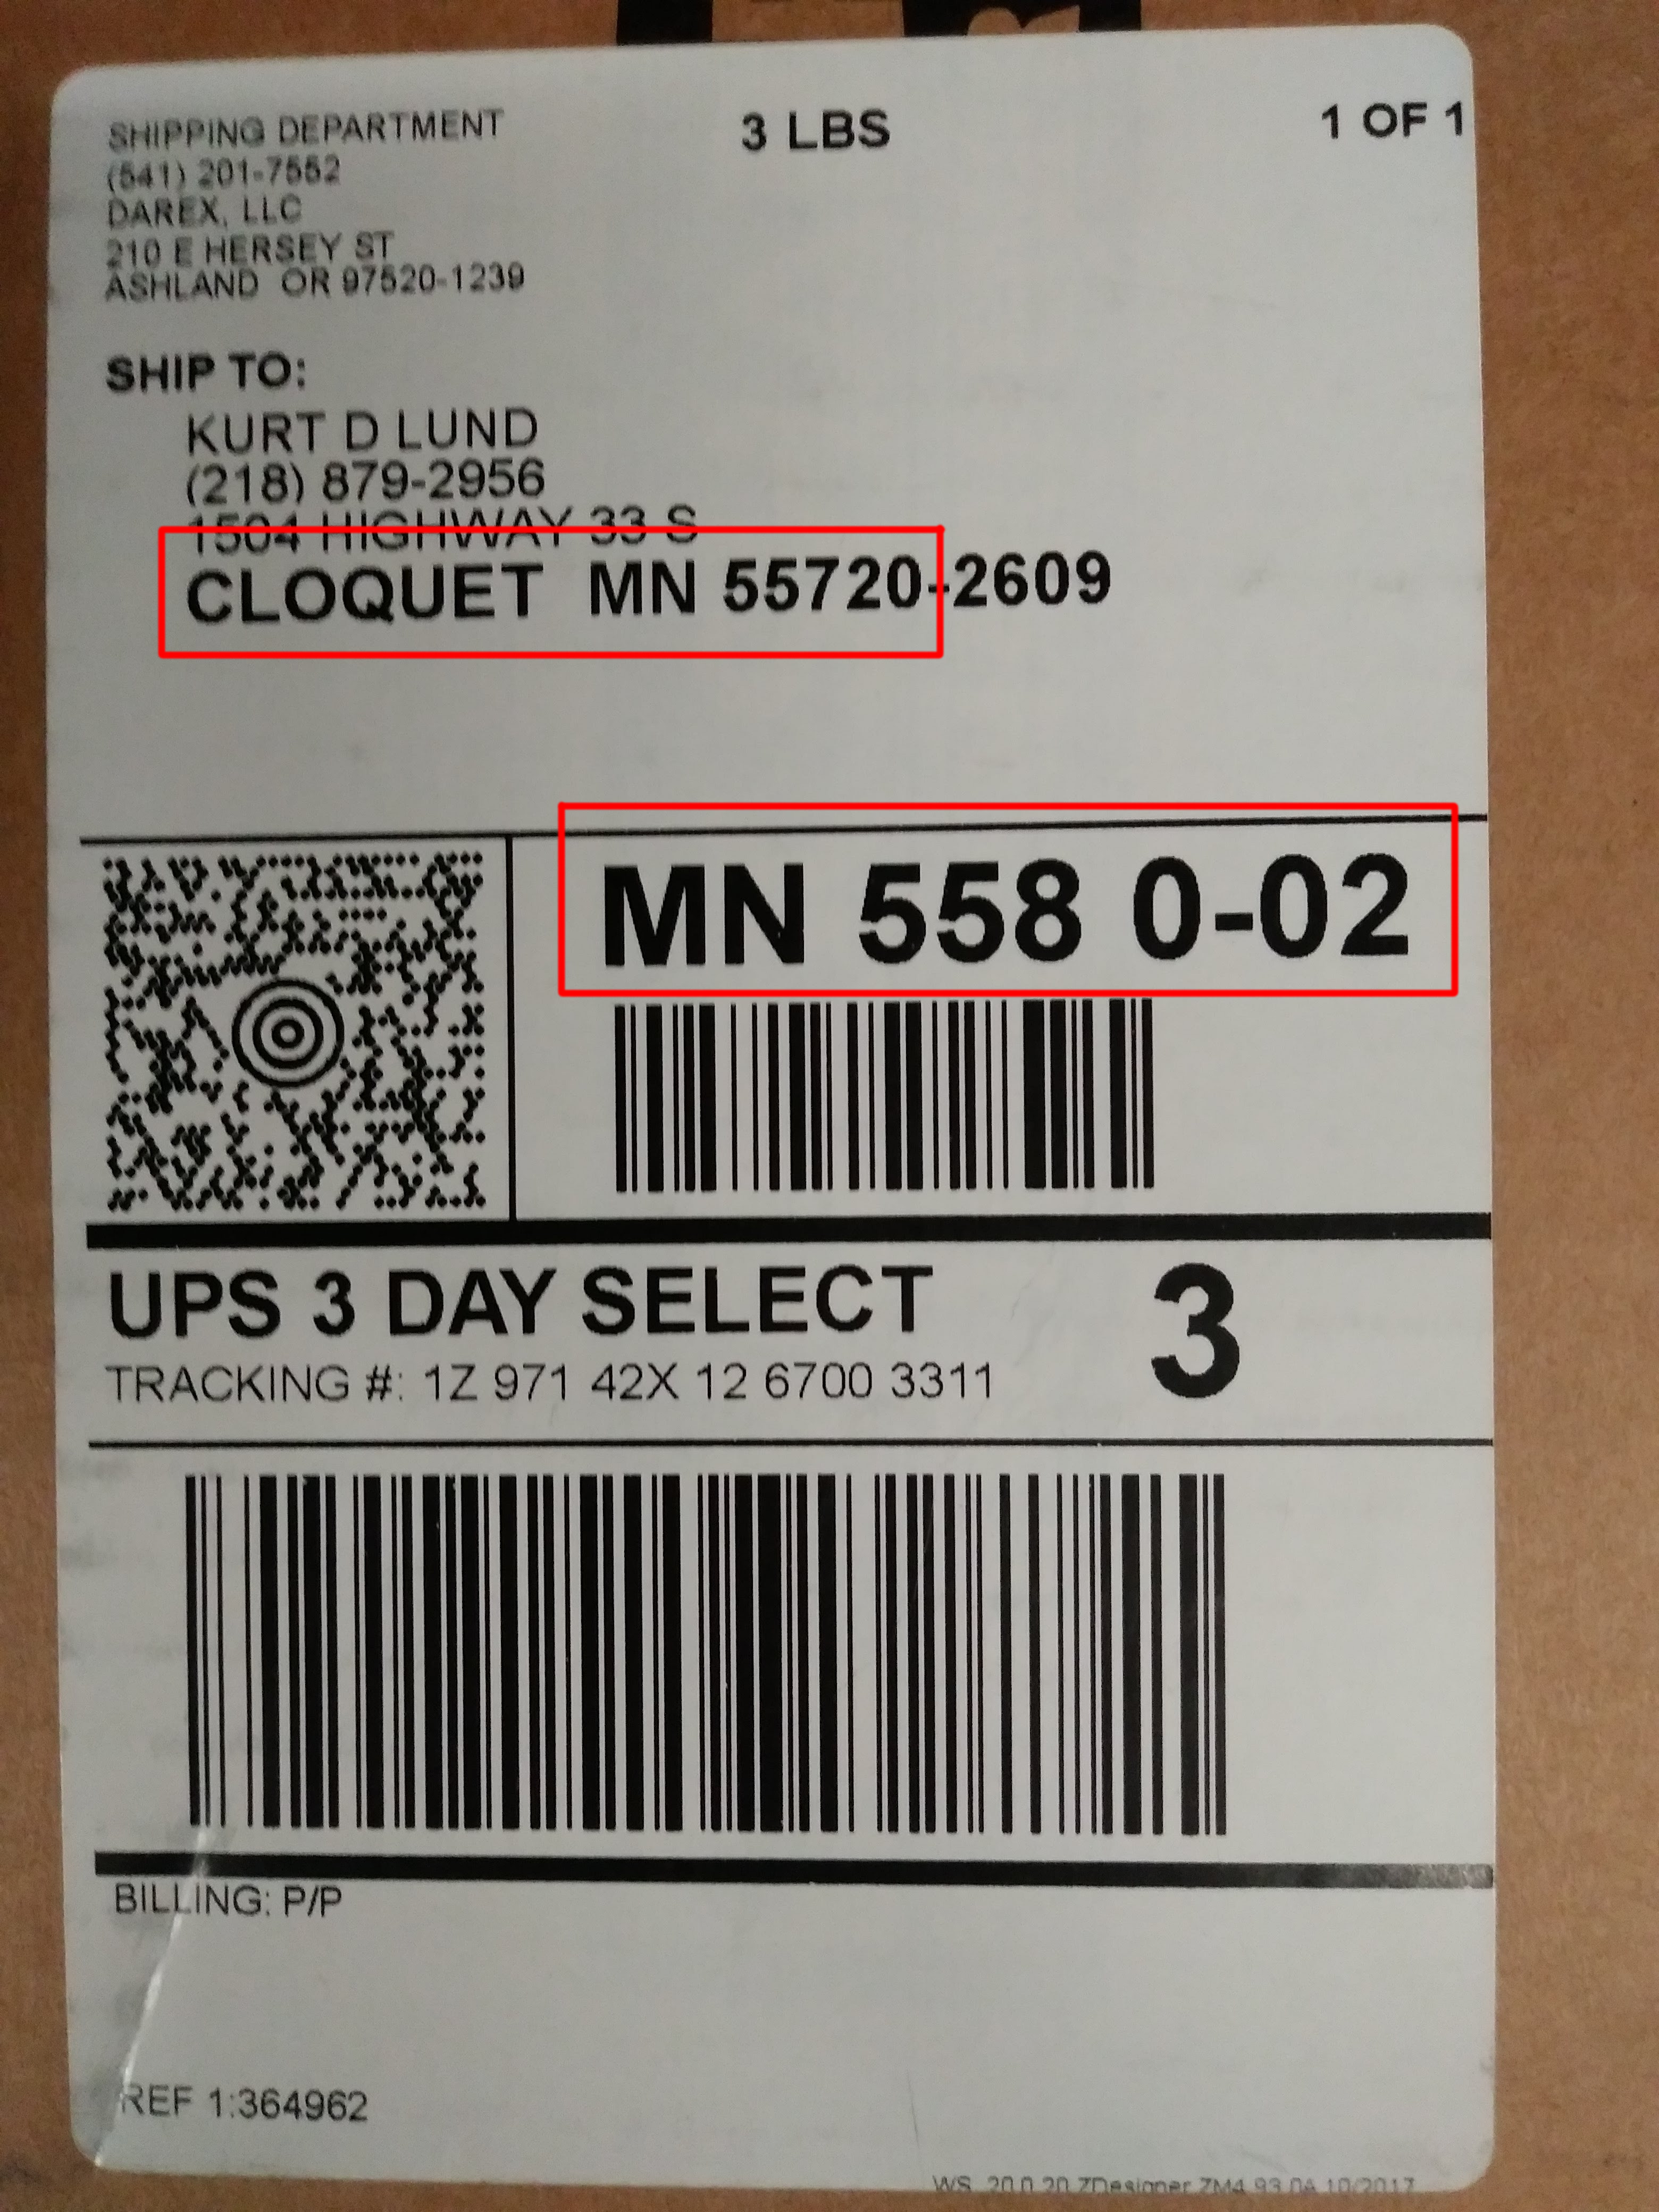
\includegraphics[width=0.5\linewidth]{20171221_161952_slic} 
\caption{SLIC and Destination}
\end{subfigure}
\begin{subfigure}{0.5\textwidth}
\centering
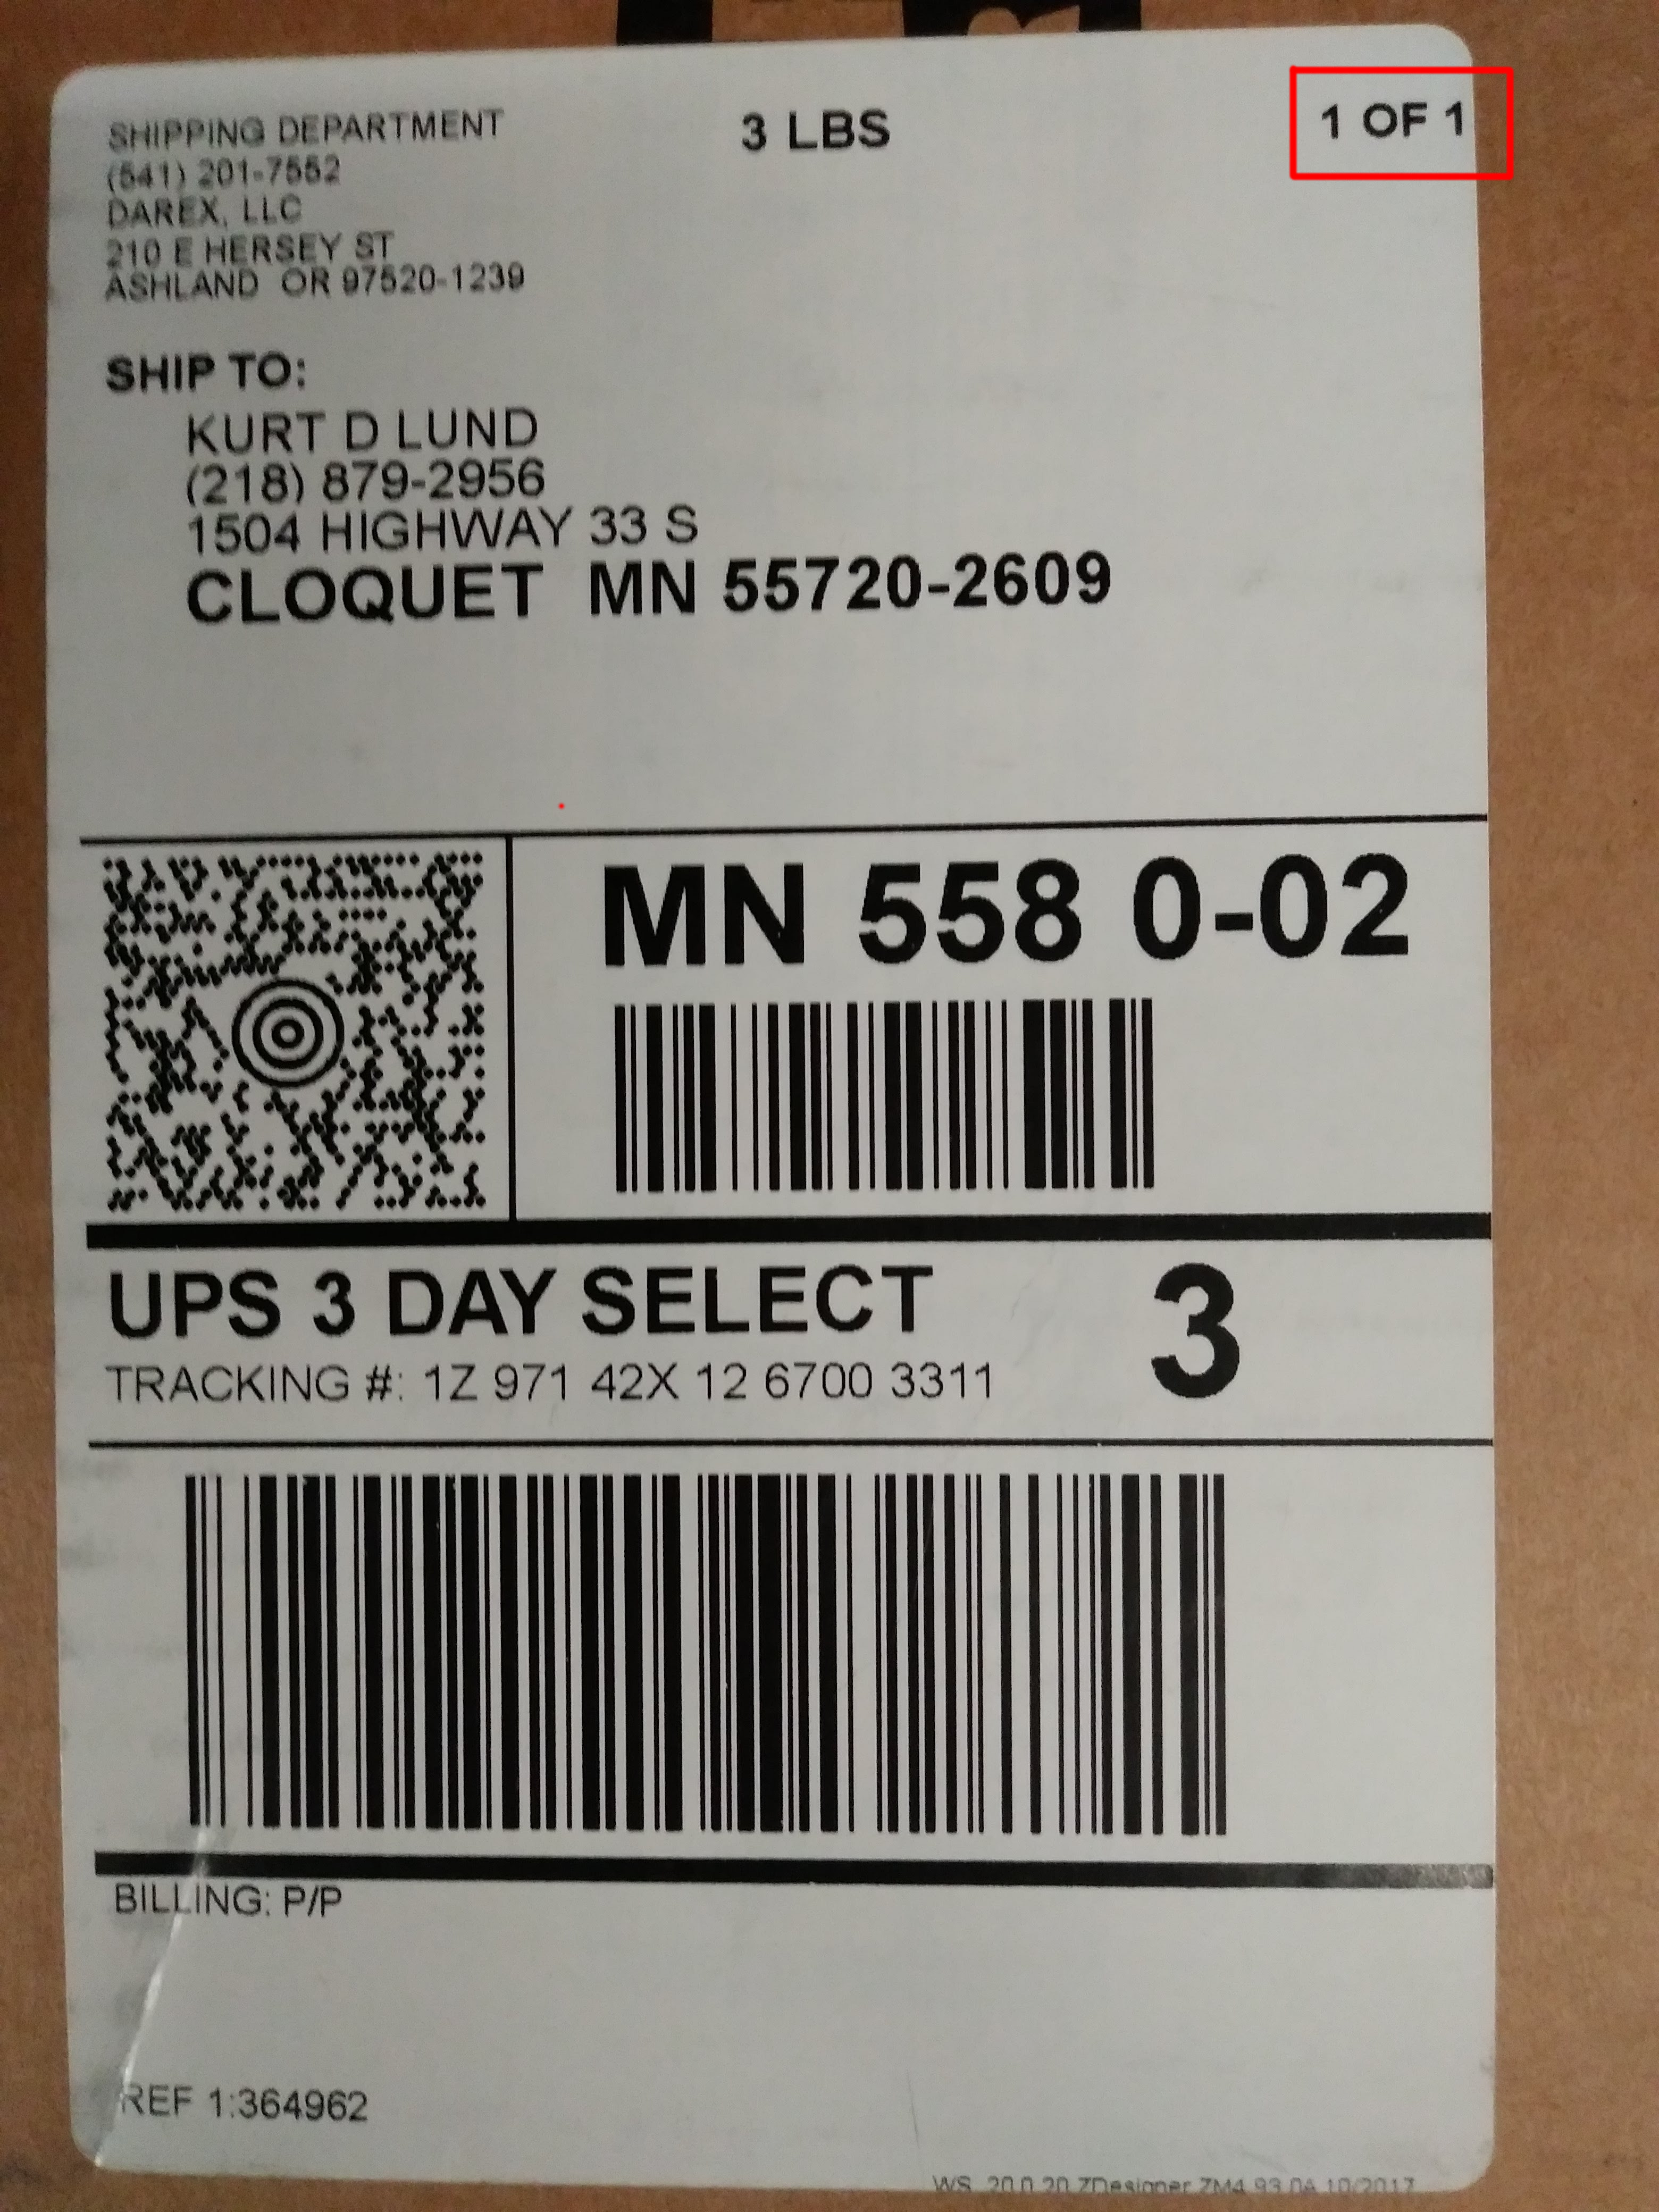
\includegraphics[width=0.5\linewidth]{20171221_161952_set}
\caption{Set/Special Count}
\end{subfigure}
\vspace{5mm}
\begin{subfigure}{0.5\textwidth}
\centering
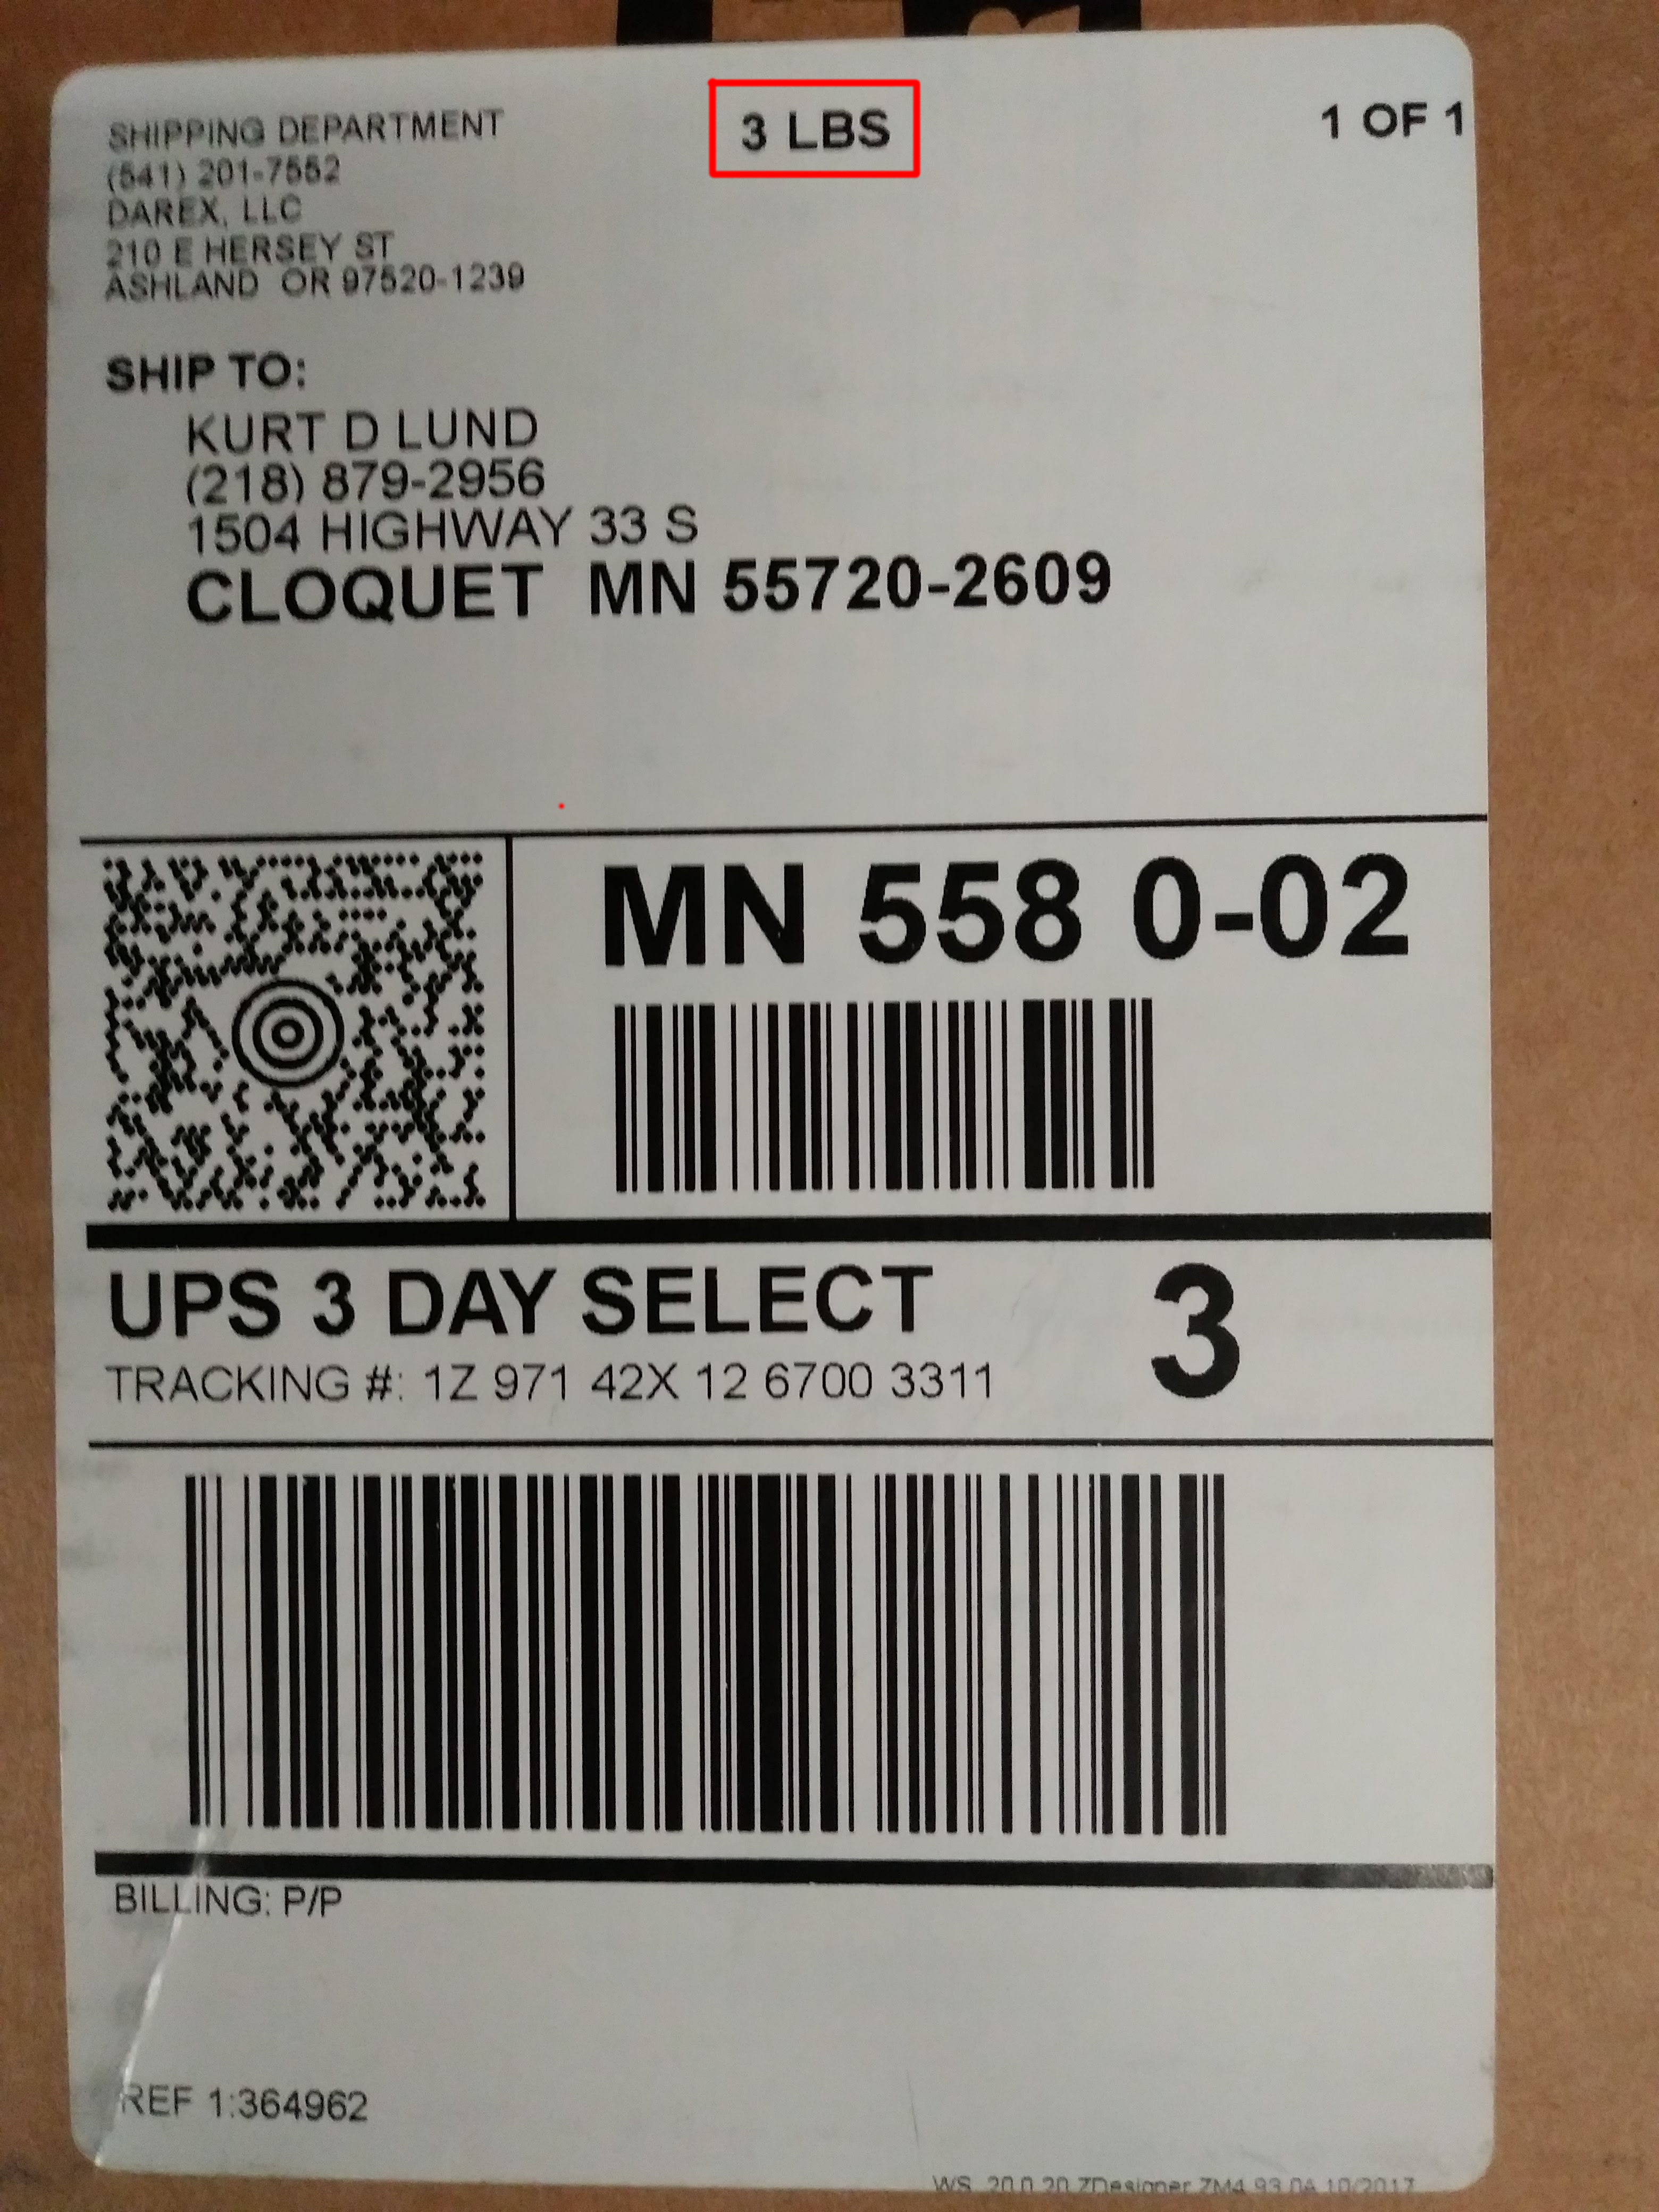
\includegraphics[width=0.5\linewidth]{20171221_161952_weight}
\caption{Weight}
\end{subfigure}
\begin{subfigure}{0.5\textwidth}
\centering
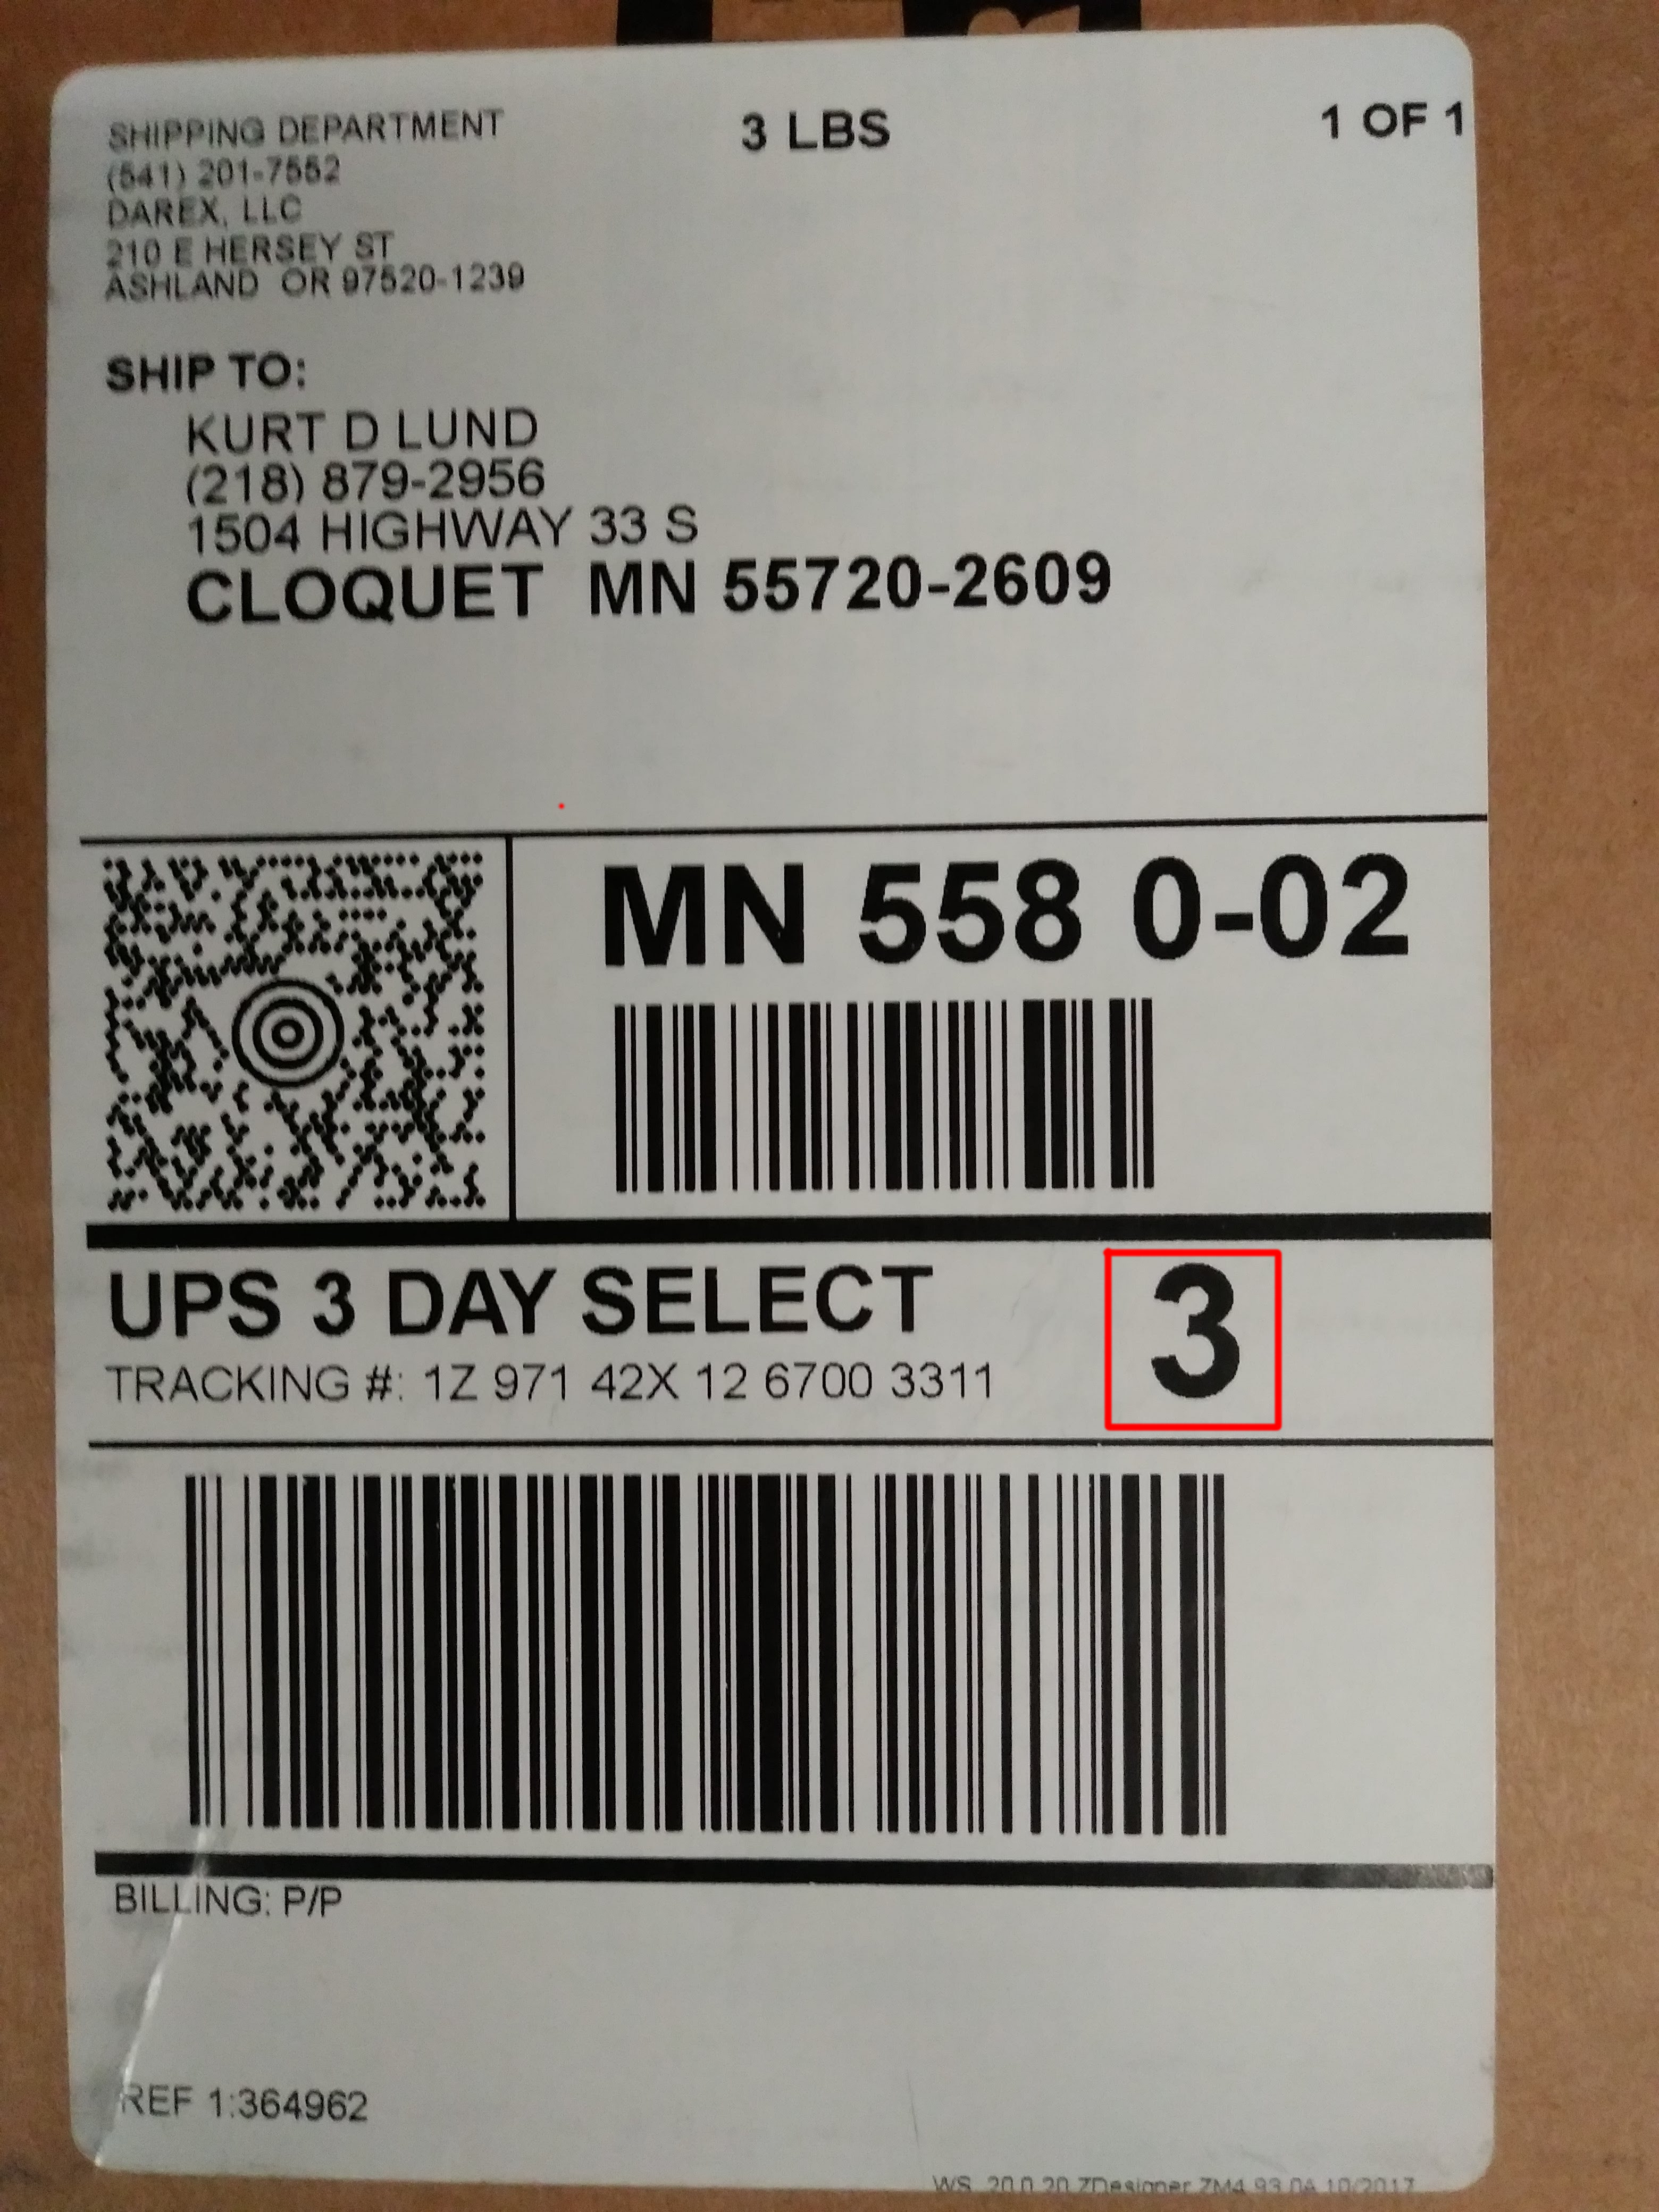
\includegraphics[width=0.5\linewidth]{20171221_161952_service.jpg}
\caption{Service Level}
\end{subfigure}
\end{figure}

\subsubsection{Exceptions}
Some states carry exception ranges where qualifying packages need to be sent to an alternate belt. On your sort reference sheet, these are the states with numbers following the state abbreviation in the US States table. 

\begin{itemize}
    \item Just like non-exception packages, the zip code in the destination address will trump the SLIC if there is a discrepancy. 
\end{itemize}

\begin{figure}[H]
    \centering
    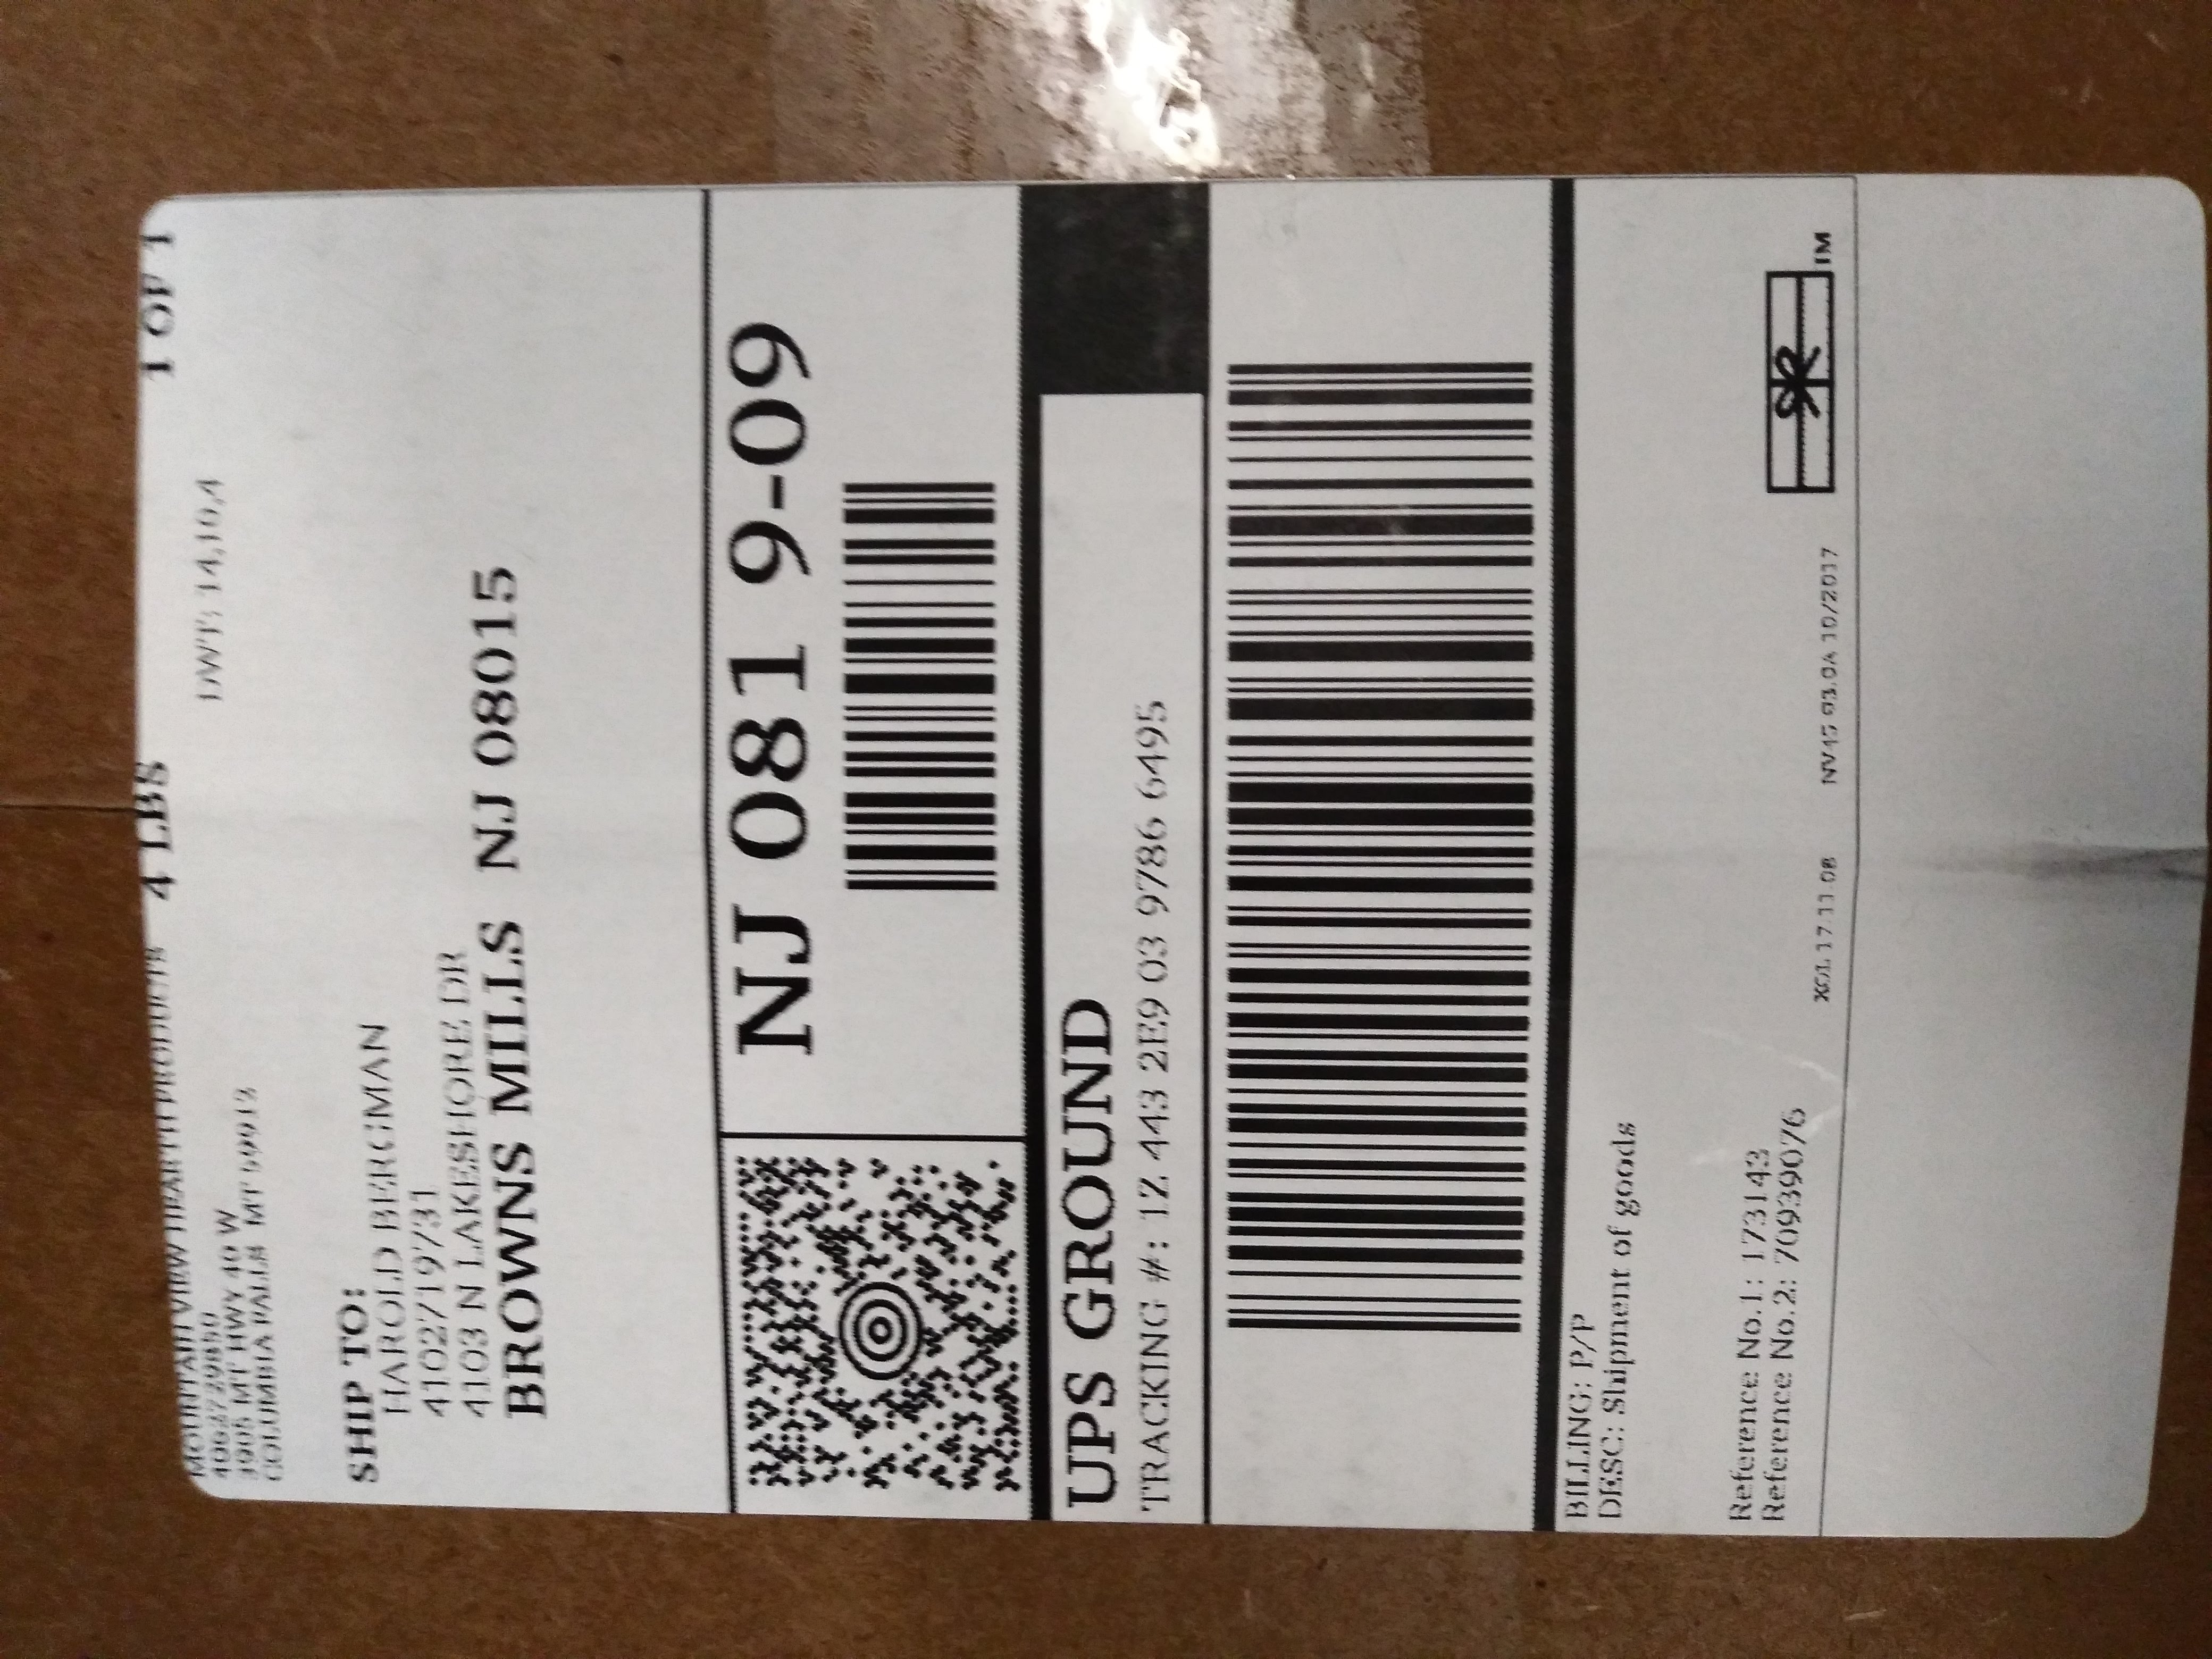
\includegraphics[width=0.4\linewidth]{20171221_161034}
    \caption{NJ 80-84 Exception}
\end{figure}

\subsubsection{Non-standard Labels}
Depending on where a package is shipped from or how it is prepared, you may receive a package that has a non-standard label.

\begin{itemize}
    \item The package must have a scannable UPS bar code at a minimum. If not, send it to re-wrap on the blue belt.
    \item Without a SLIC or standard label, make your best assessment of the destination address to determine the proper belt.
\end{itemize}

\begin{figure}[H]
\begin{subfigure}{0.5\textwidth}
\centering
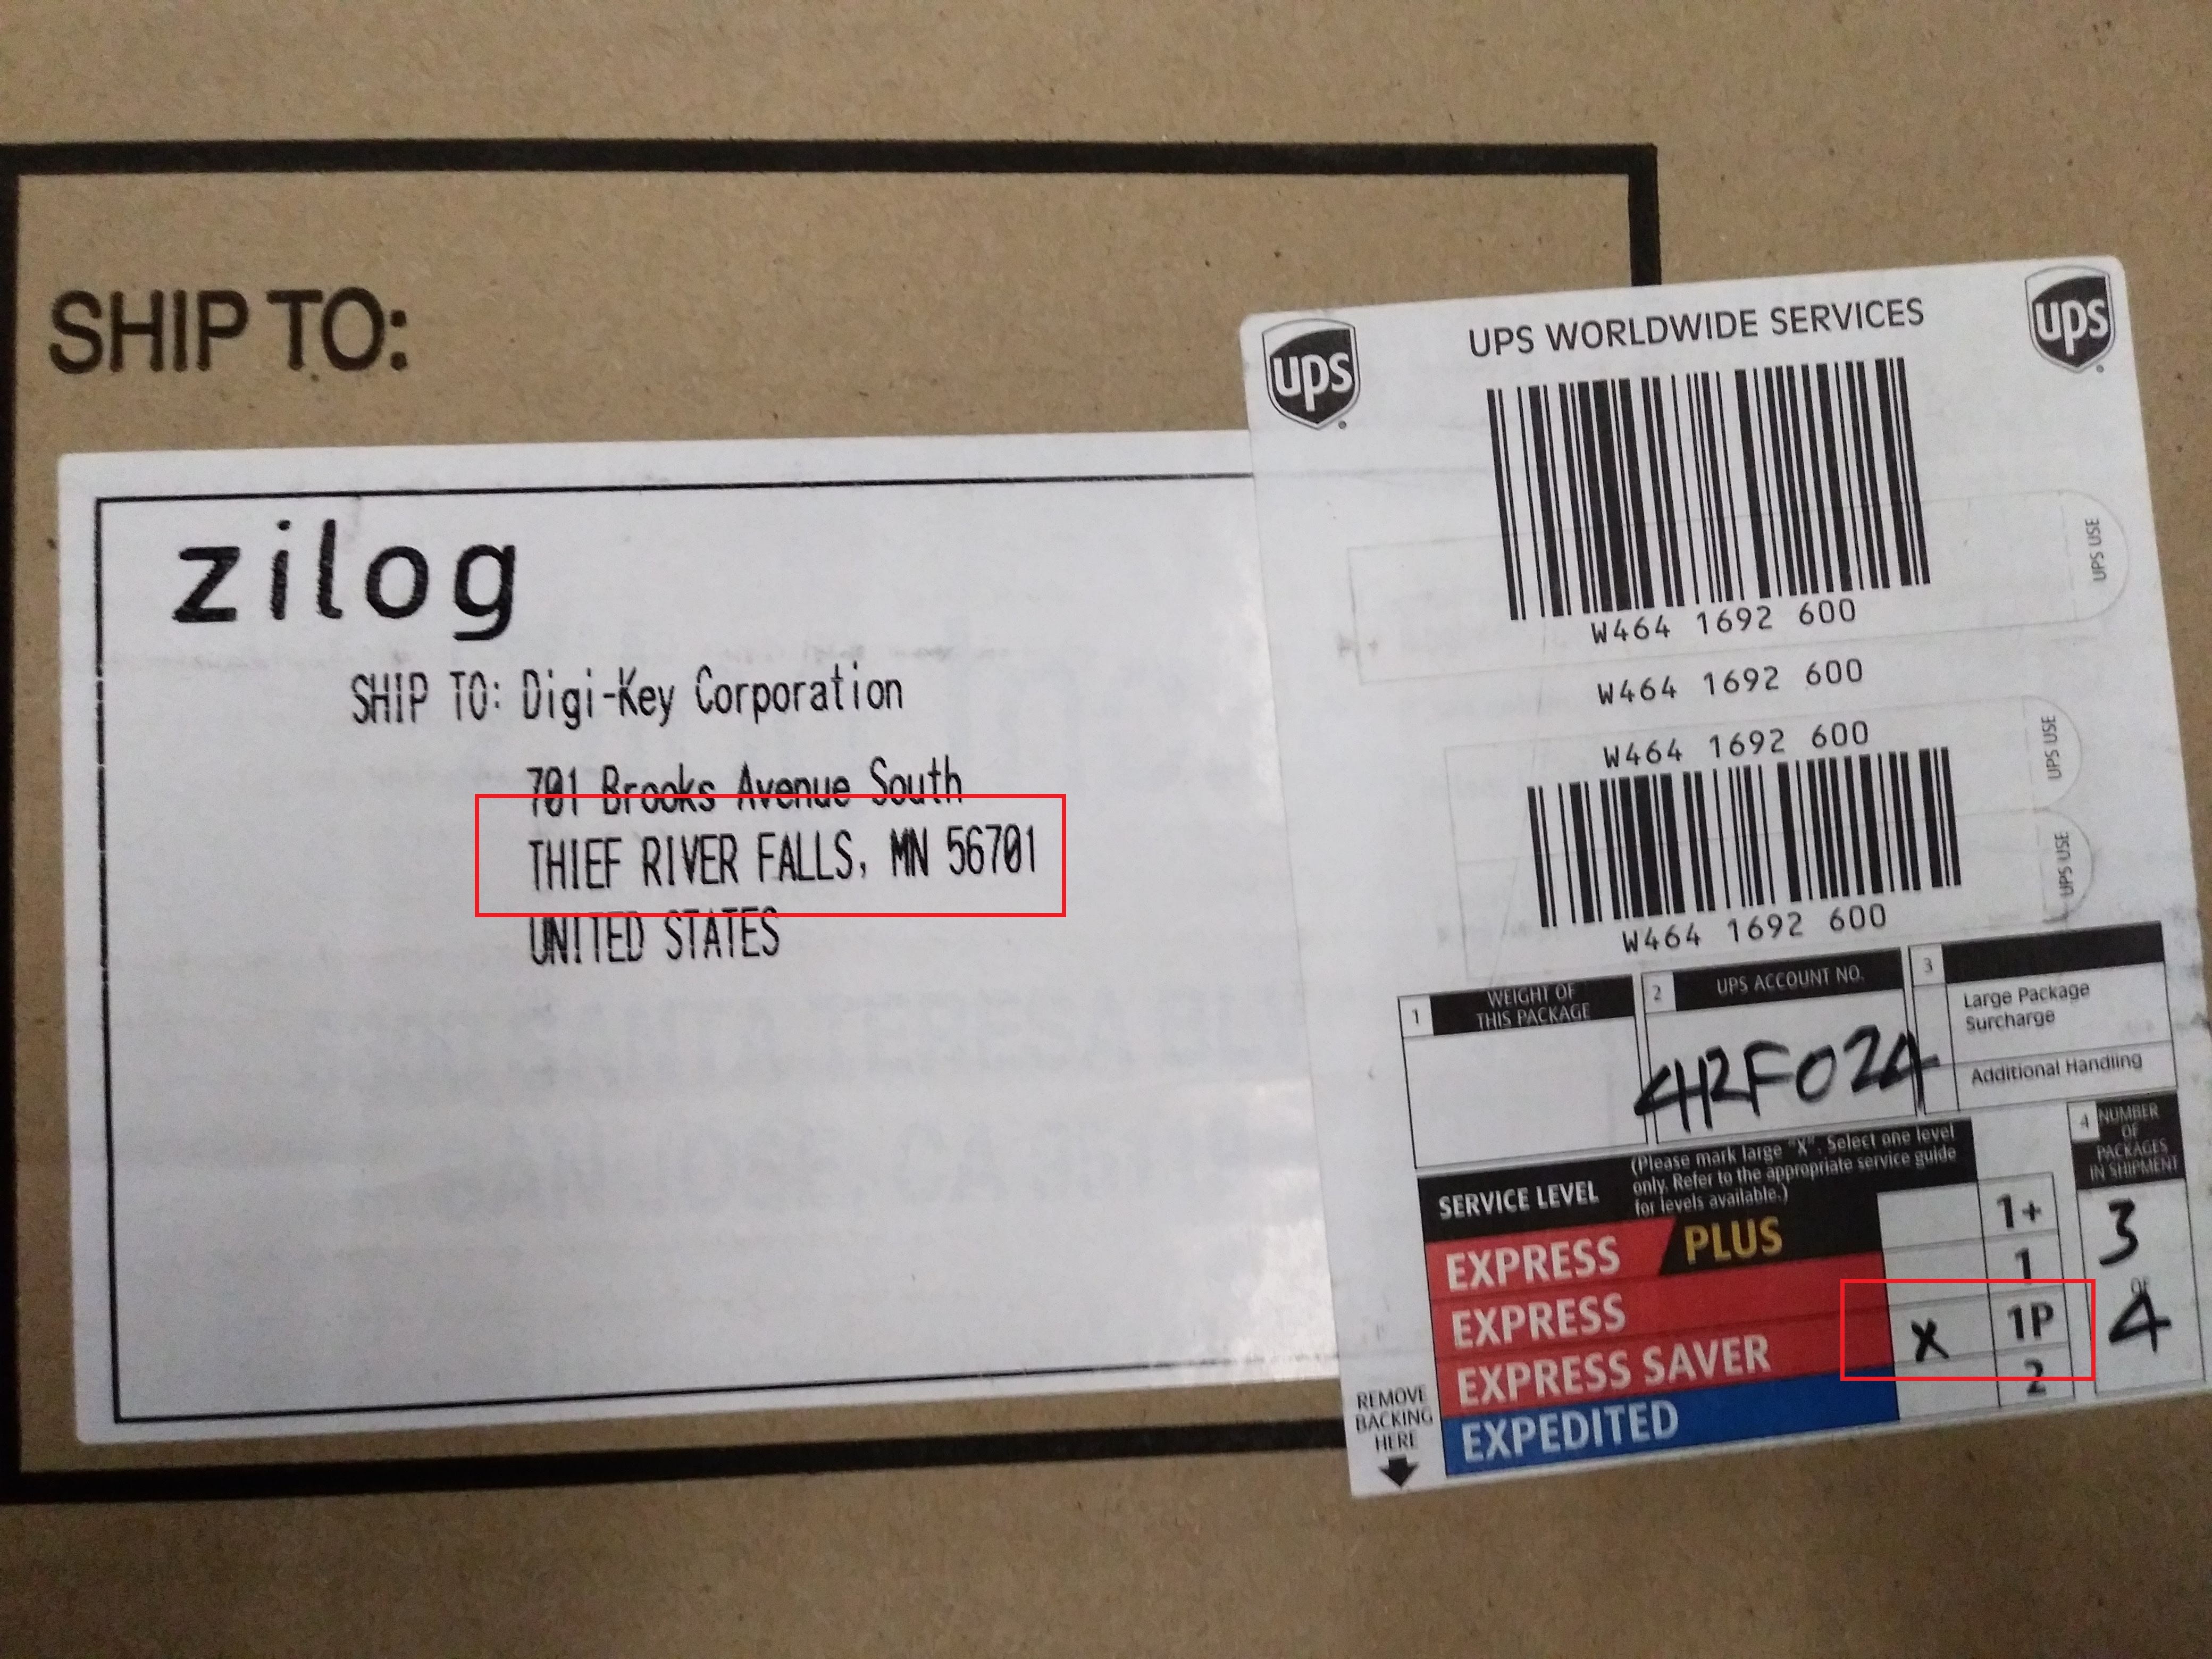
\includegraphics[width=0.7\linewidth]{20171221_193129}
\caption{}
\end{subfigure}
\vspace{5mm}
\begin{subfigure}{0.5\textwidth}
\centering
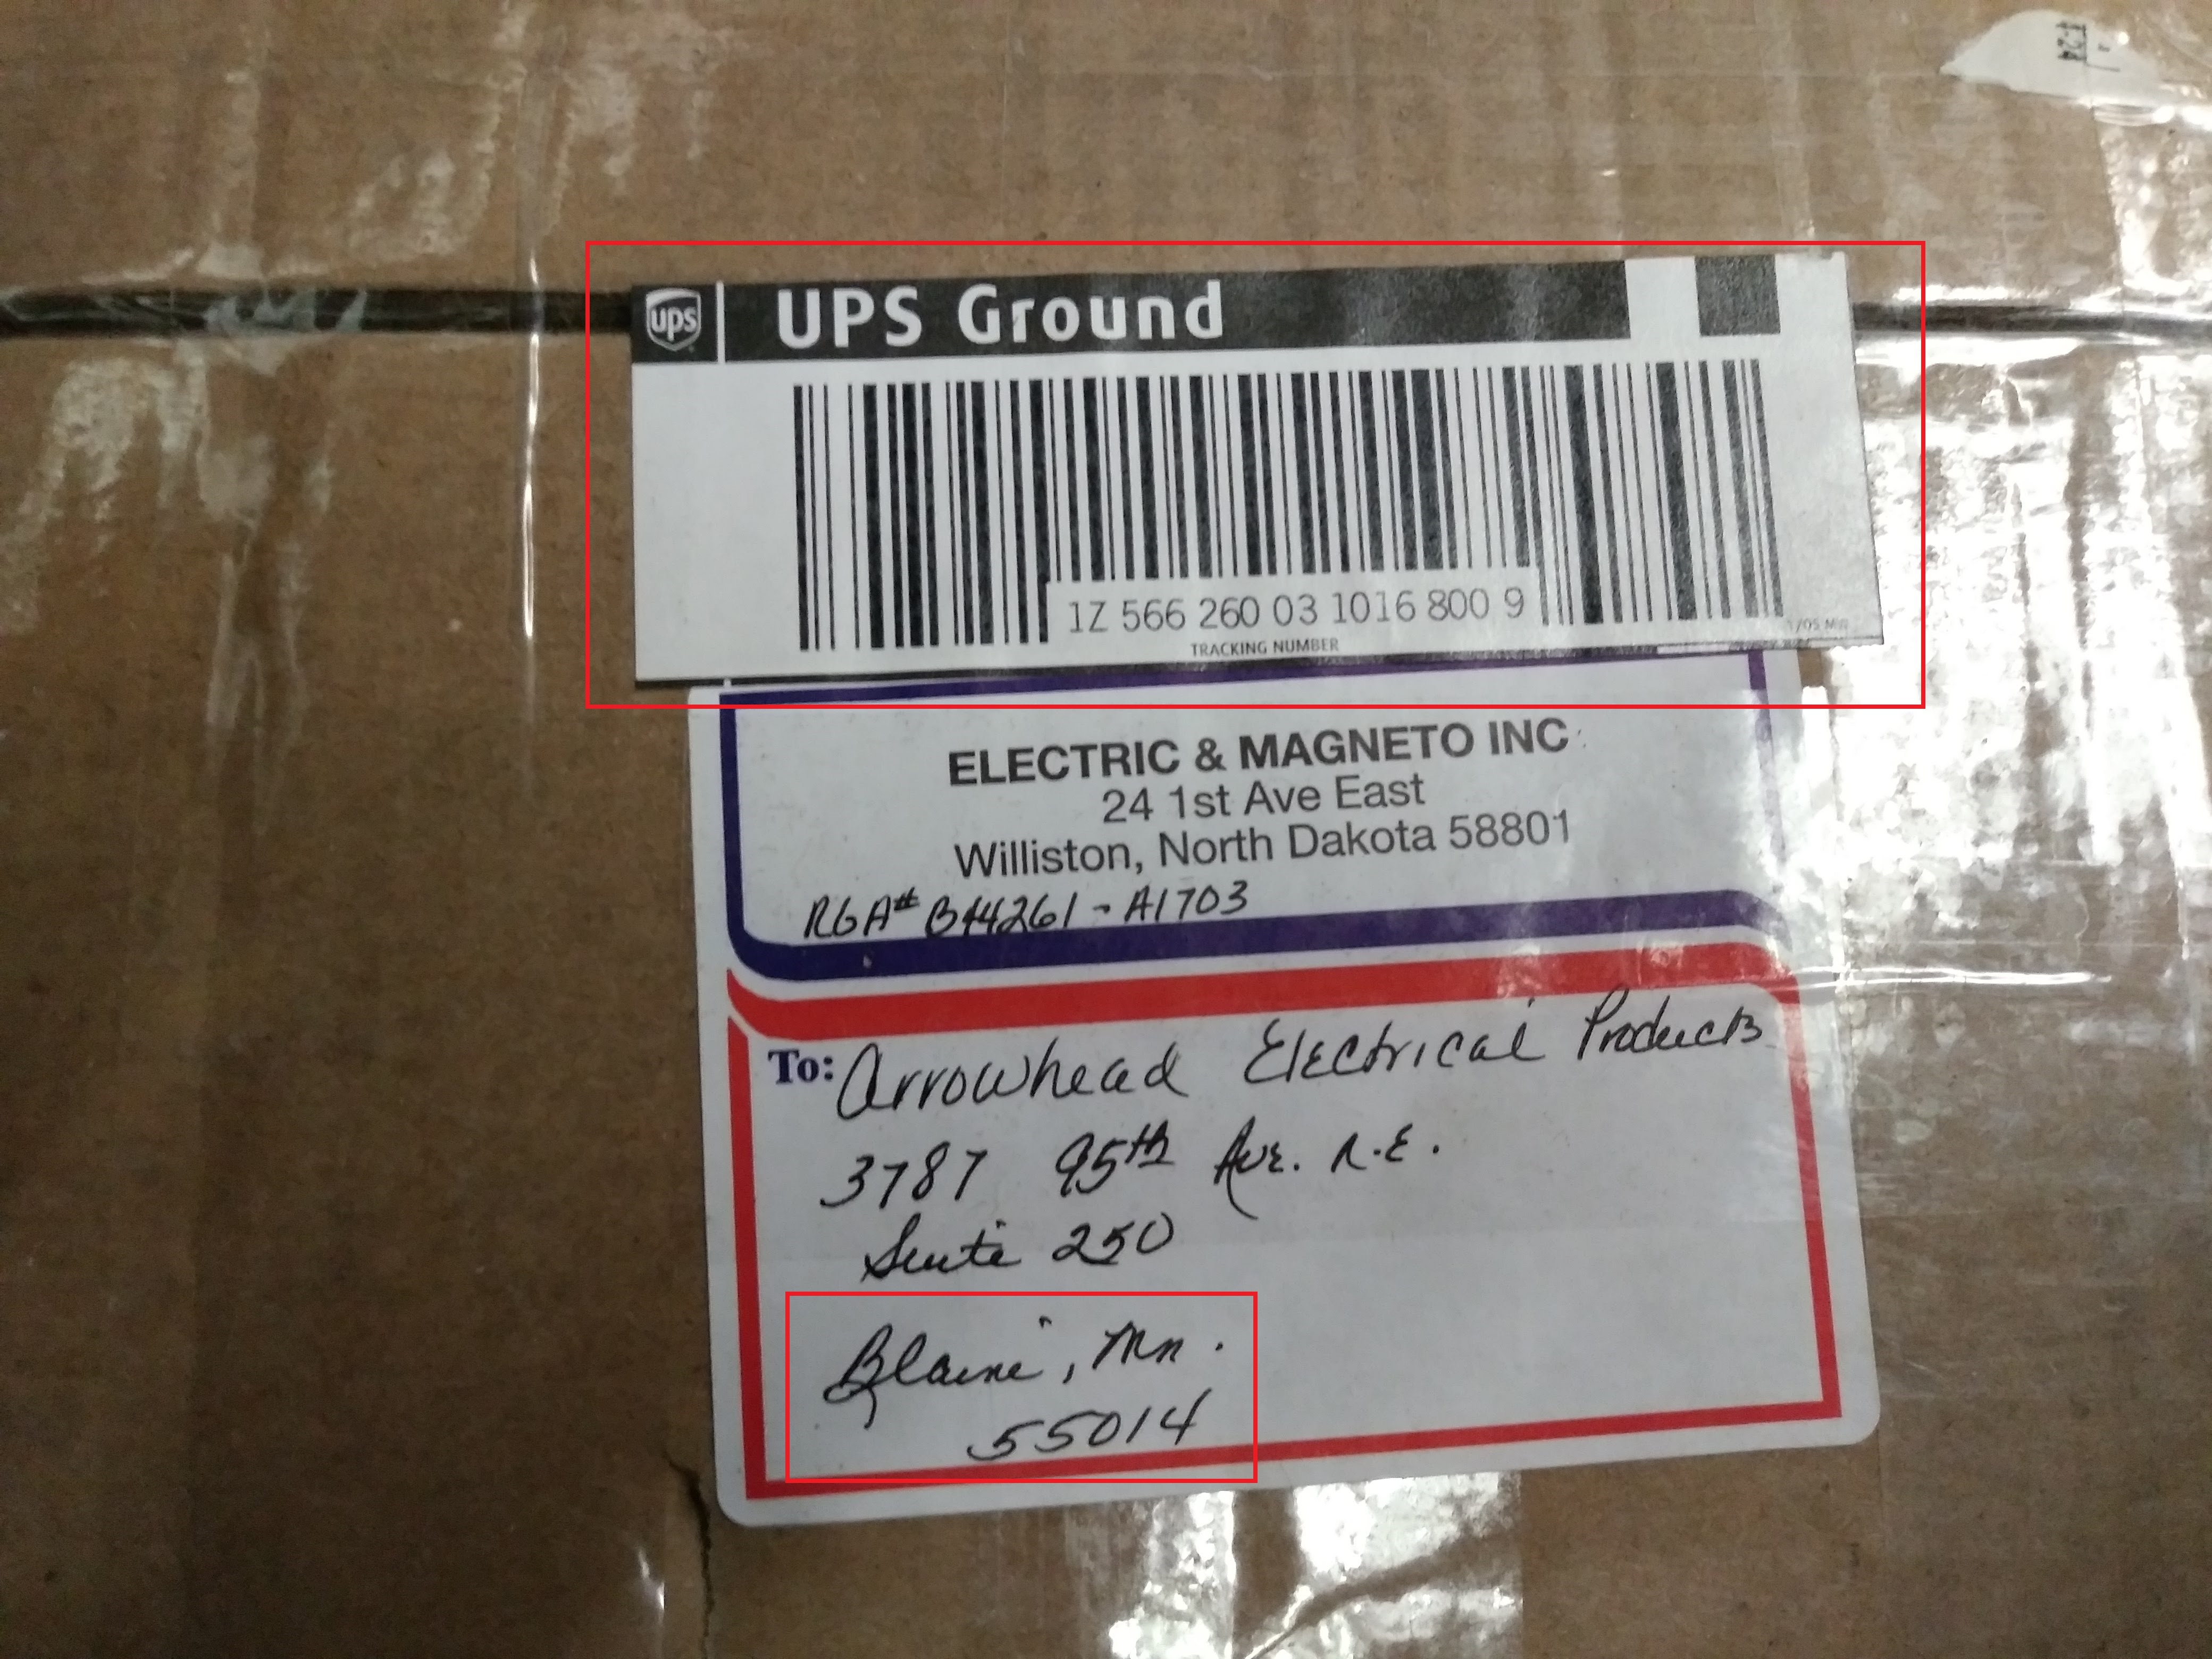
\includegraphics[width=0.7\linewidth]{20171221_183147}
\caption{}
\end{subfigure}
\end{figure}
\clearpage
\subsubsection{Bags}
A significant percentage of UPS' volume is transported having been containerized with several other packages. These are called "smalls" and are processed by the small sort area. Ultimately, the more volume that small sort can handle the better since this reduces damages and processing time for the system.

\begin{itemize}
    \item If a bag has a SLIC then sort it accordingly.
    \item Bags that lack a SLIC have not been processed by a small sort. If the destination lists "Minneapolis" or "Saint Paul" those can be processed by our facility and should go to the small sort belt.
    \item If a bag lists a destination other than Minneapolis or Saint Paul then sort it accordingly.
    \item If a bag does not have a label it should go to the small sort belt.
\end{itemize}

\begin{figure}[H]
\begin{subfigure}{0.5\textwidth}
\centering
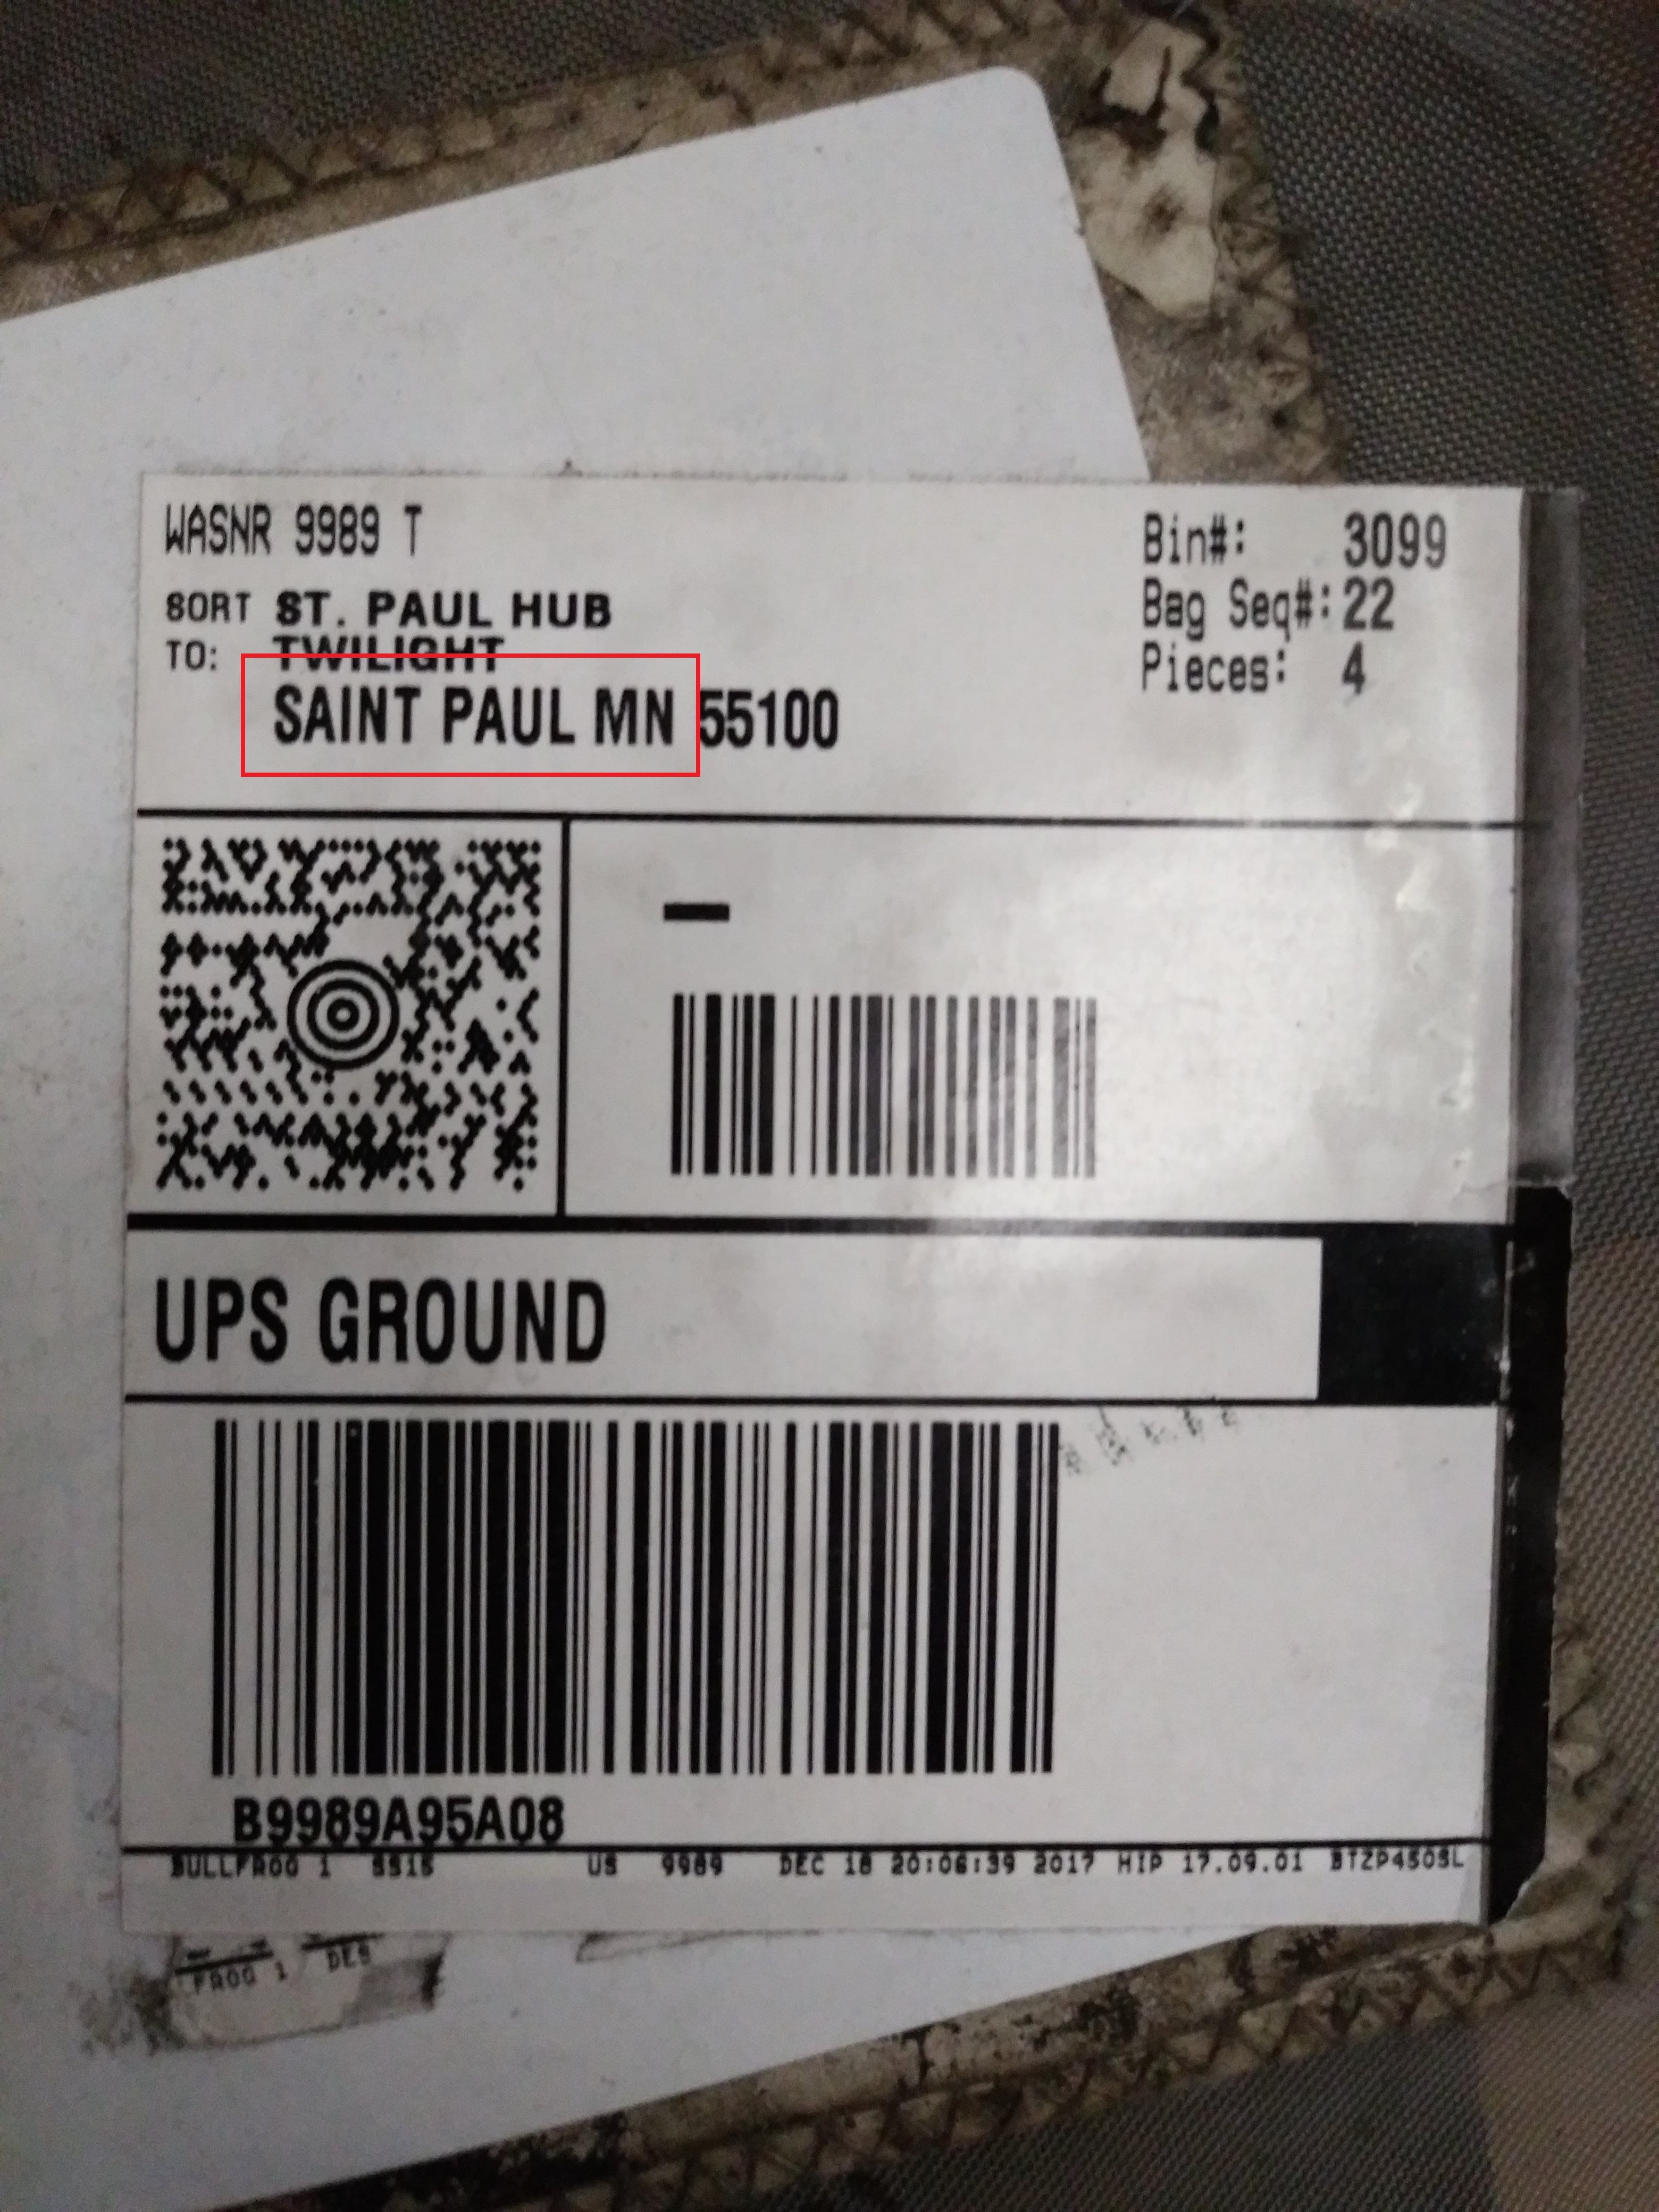
\includegraphics[width=0.5\linewidth]{20171221_171159} 
\caption{Bag Label - No SLIC}
\end{subfigure}
\begin{subfigure}{0.5\textwidth}
\centering
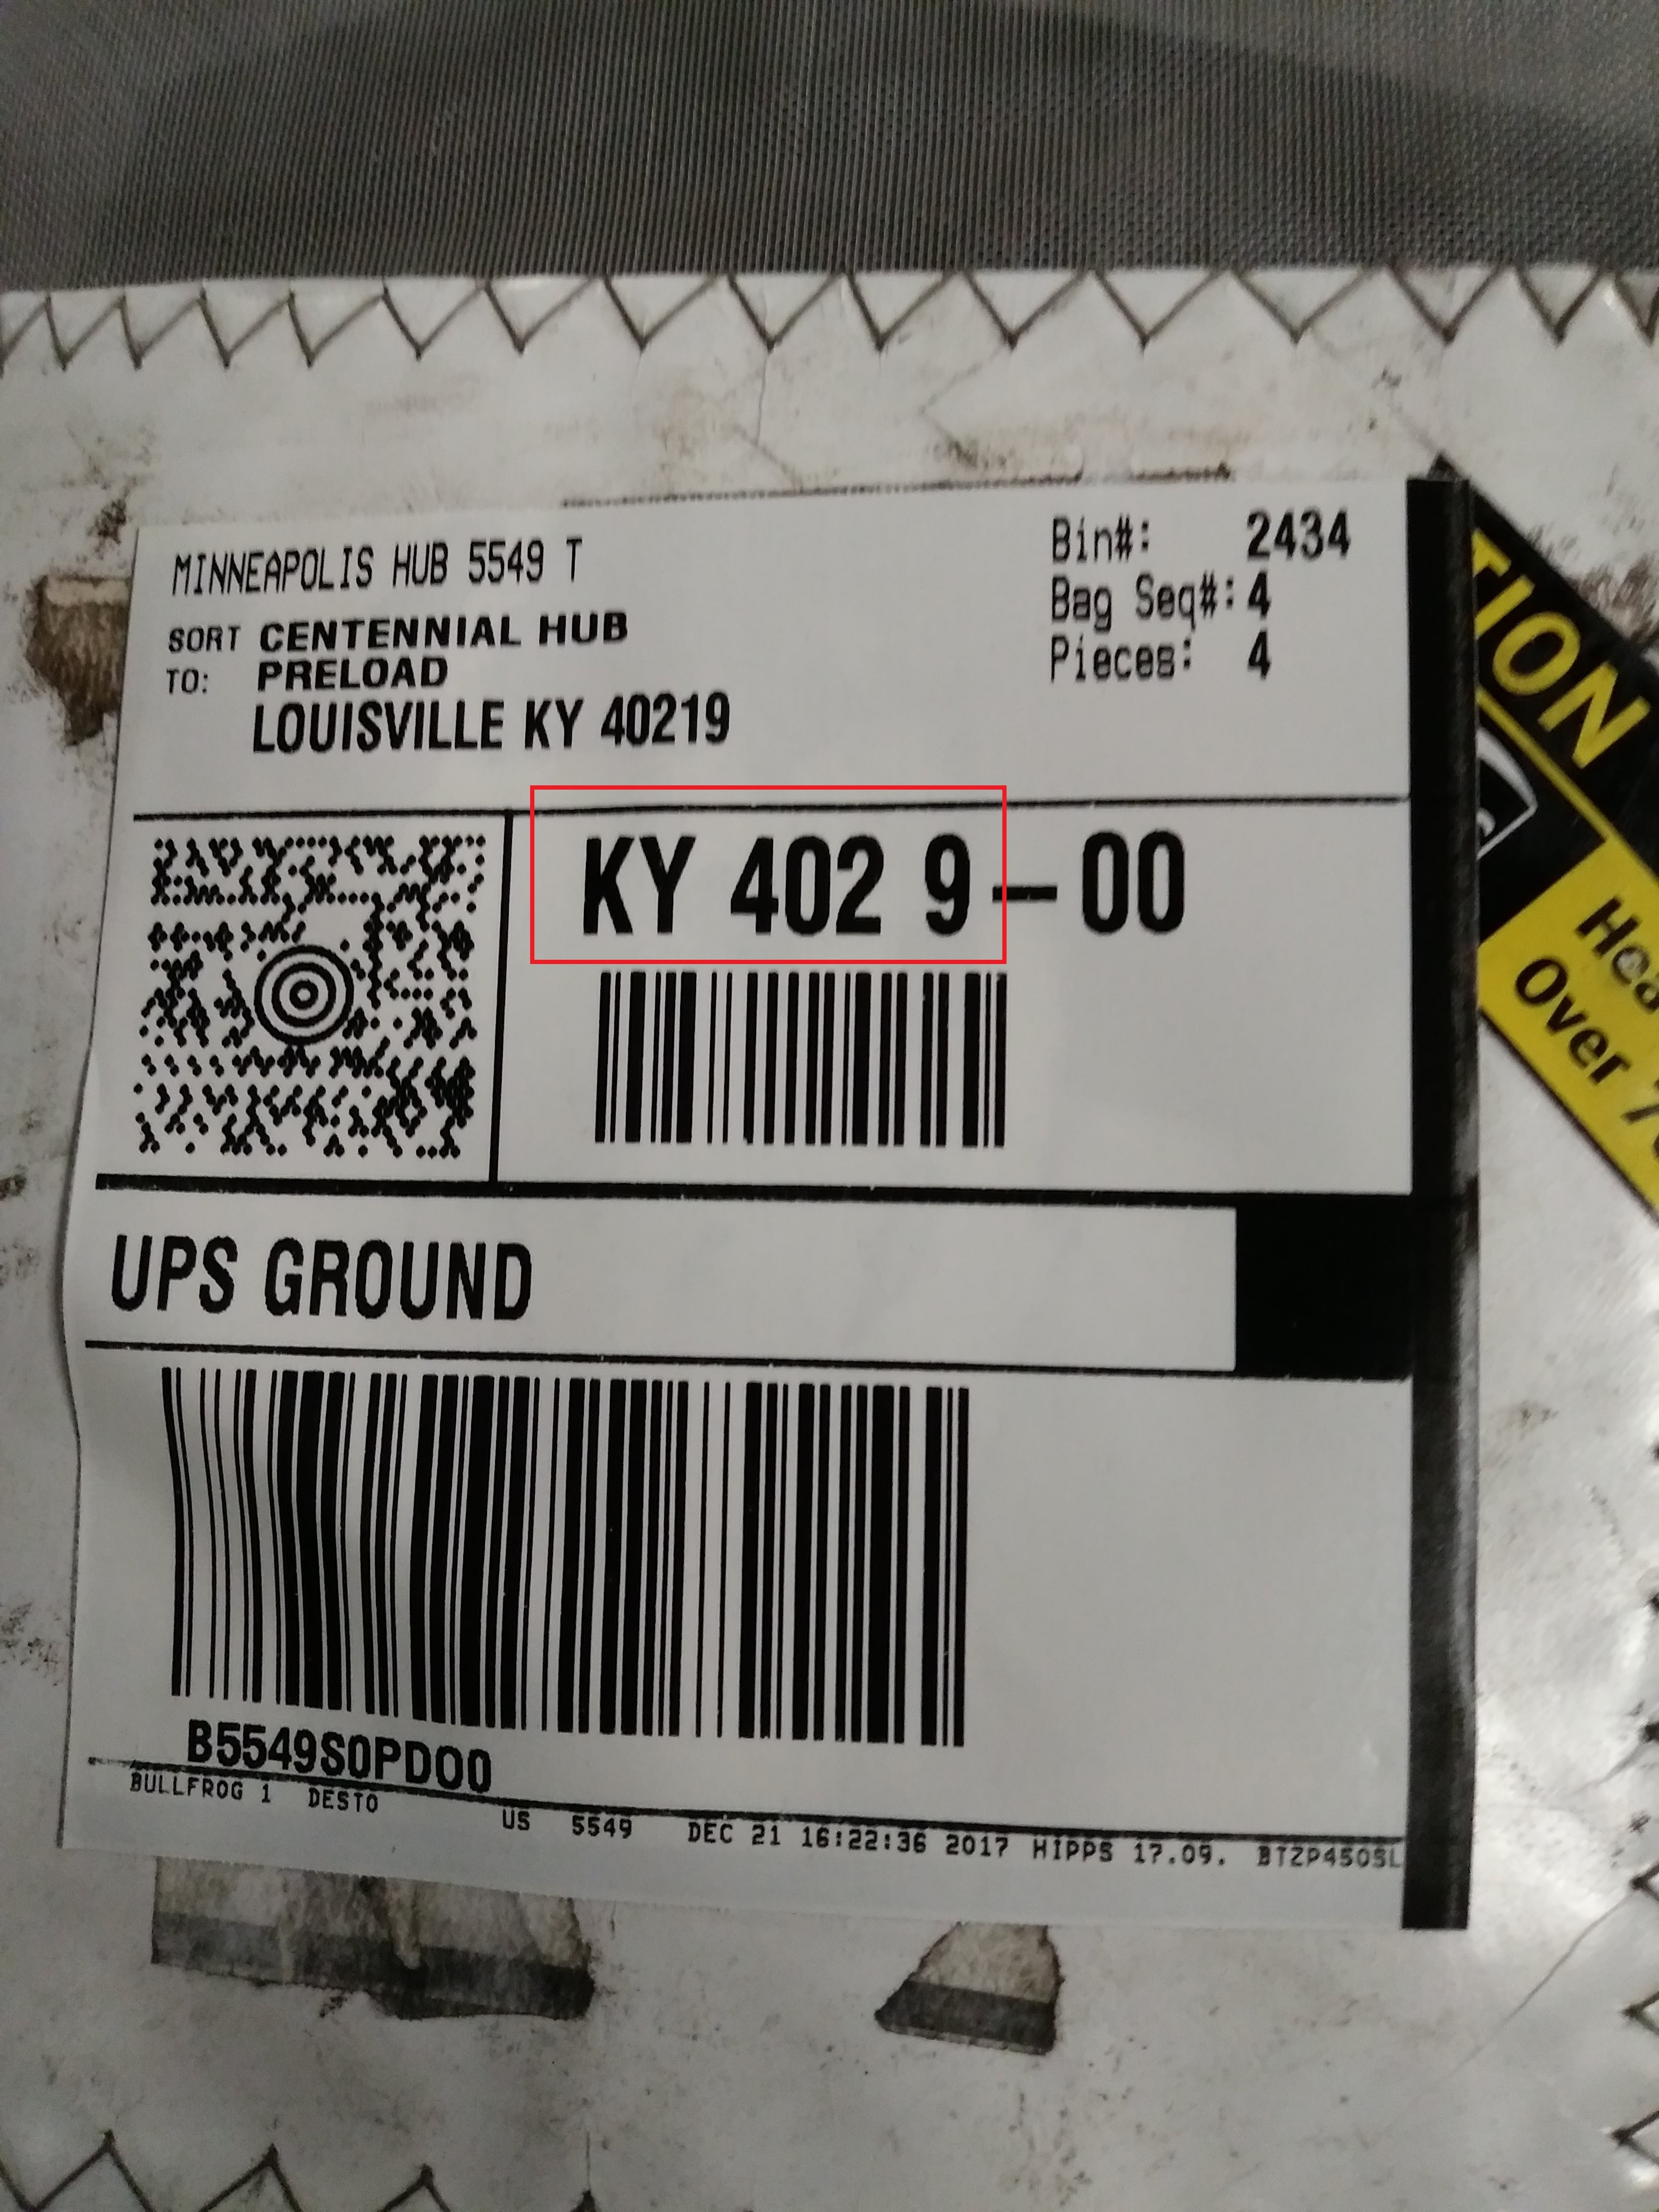
\includegraphics[width=0.5\linewidth]{20171221_162712}
\caption{Passthrough Bag - With SLIC}
\end{subfigure}
\vspace{5mm}
\begin{subfigure}{0.5\textwidth}
\centering
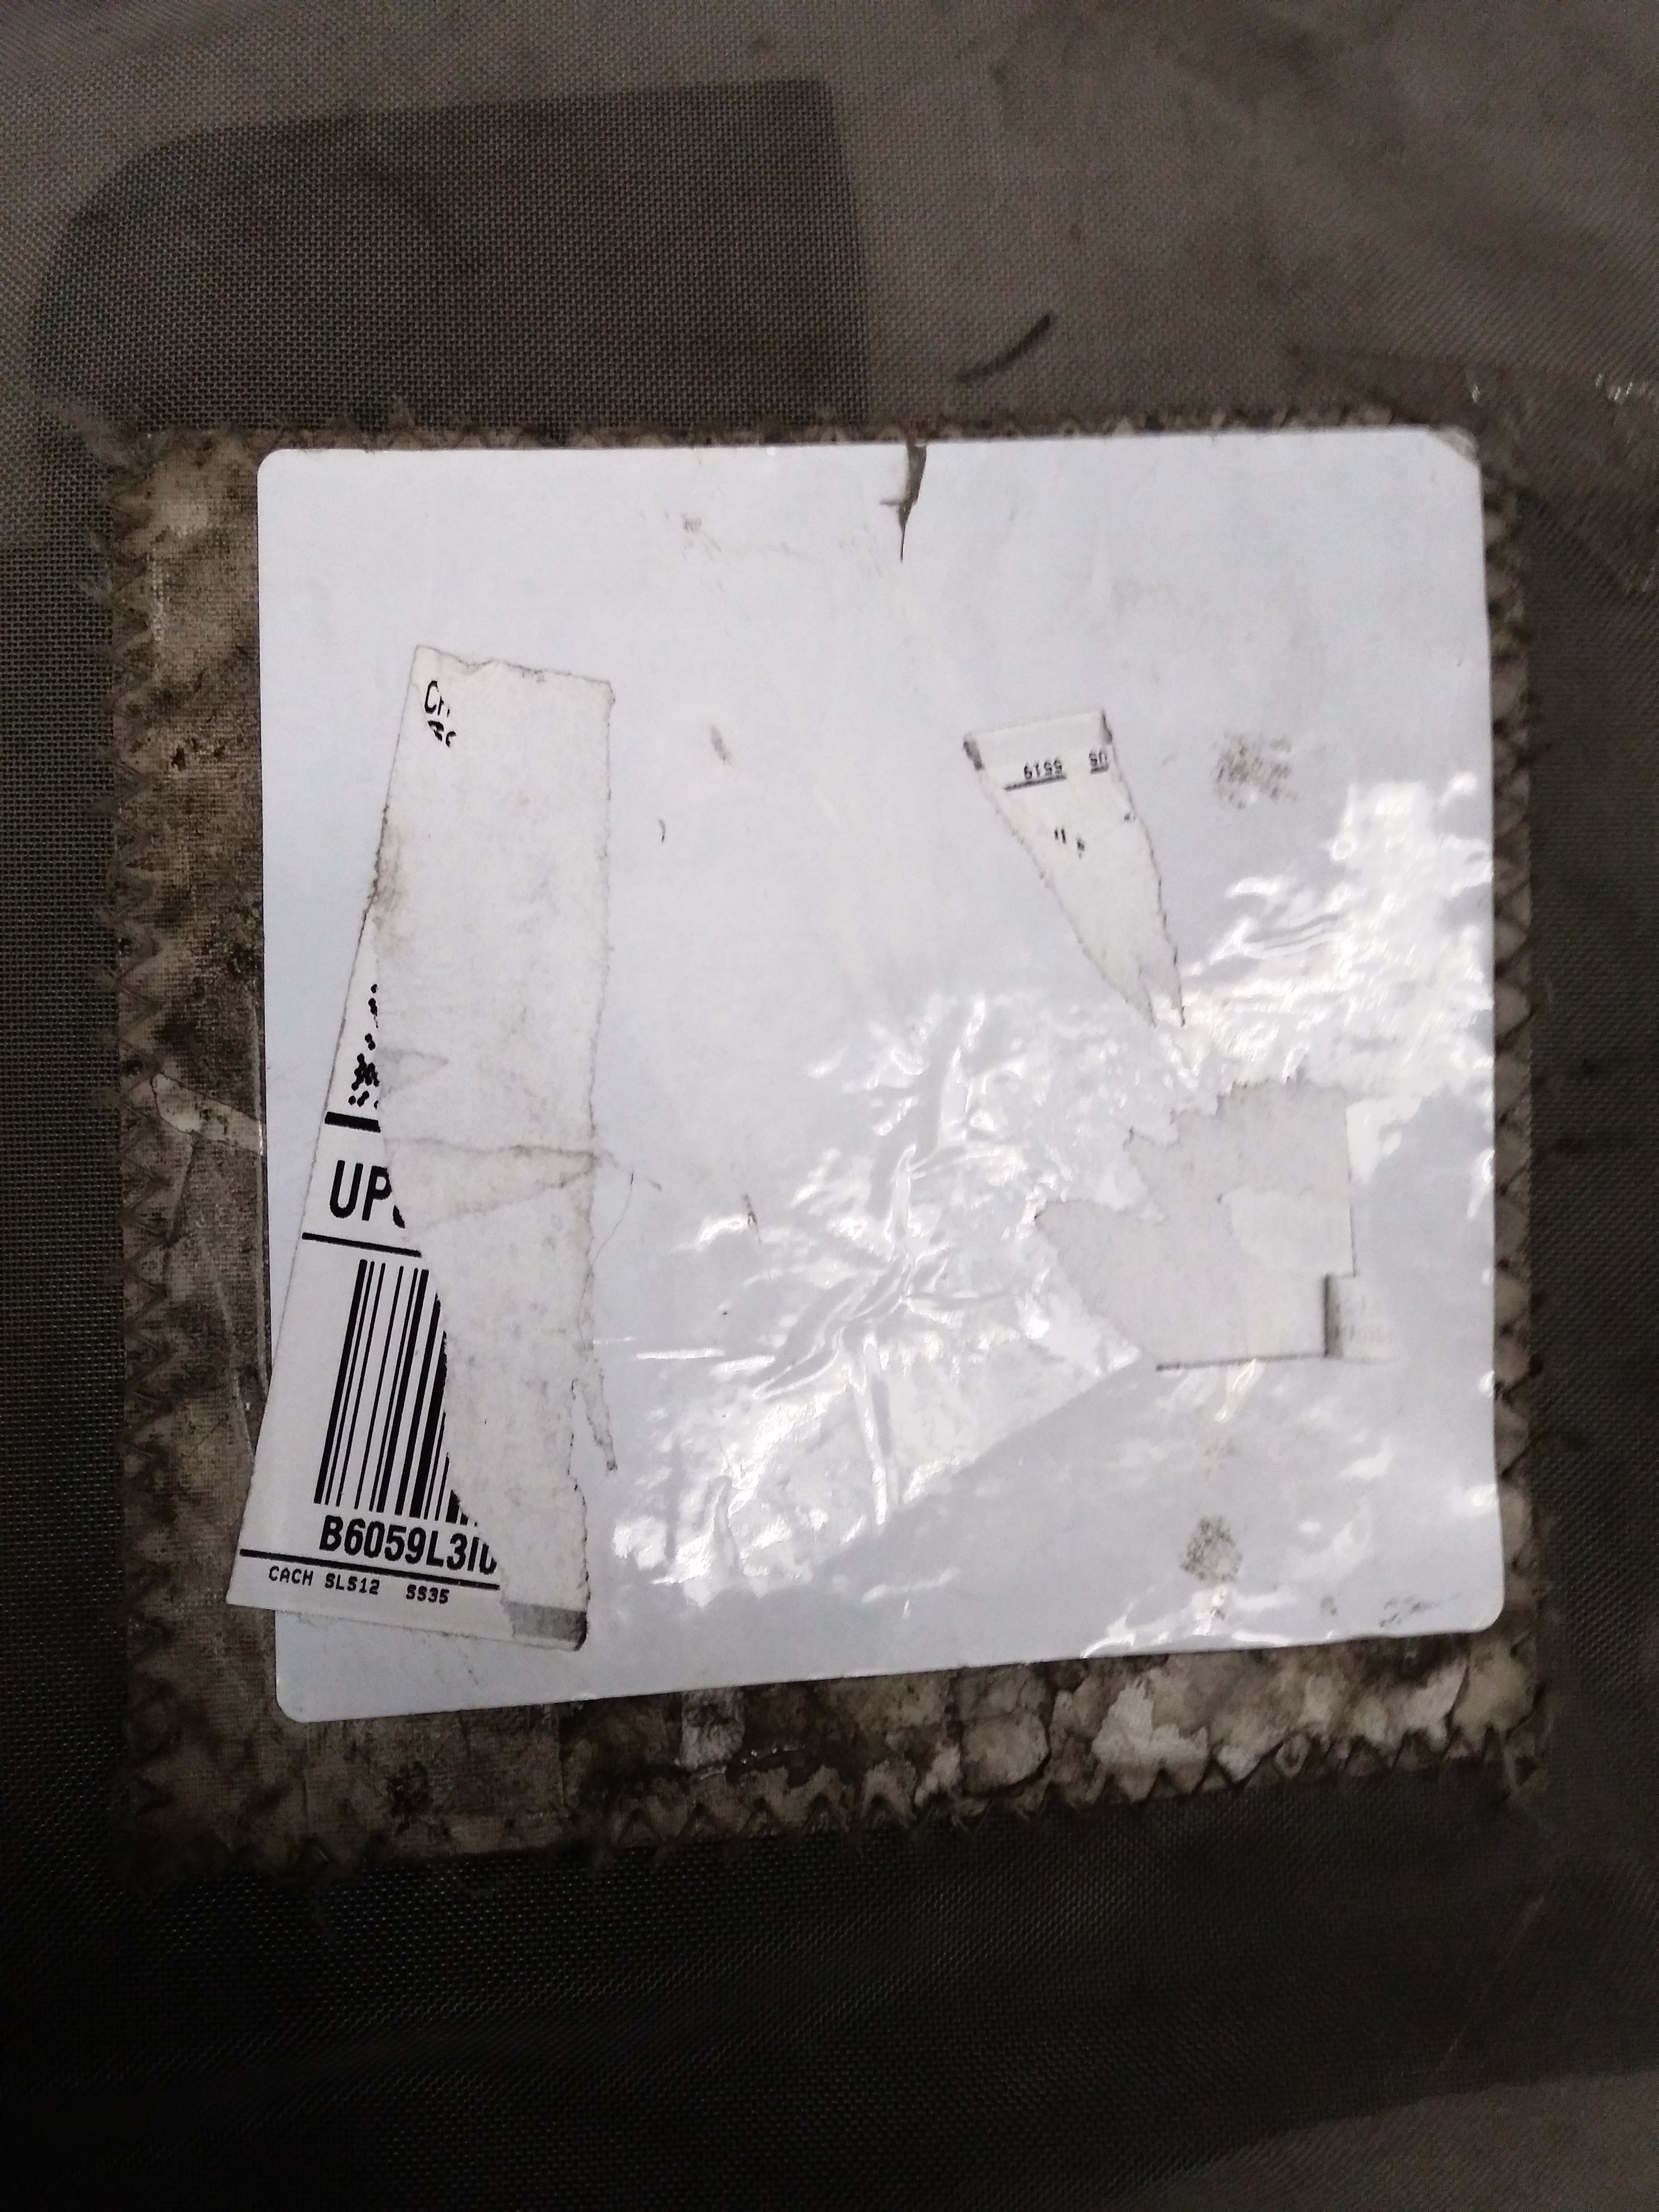
\includegraphics[width=0.5\linewidth]{20171221_161027}
\caption{No Label}
\end{subfigure}
\begin{subfigure}{0.5\textwidth}
\centering
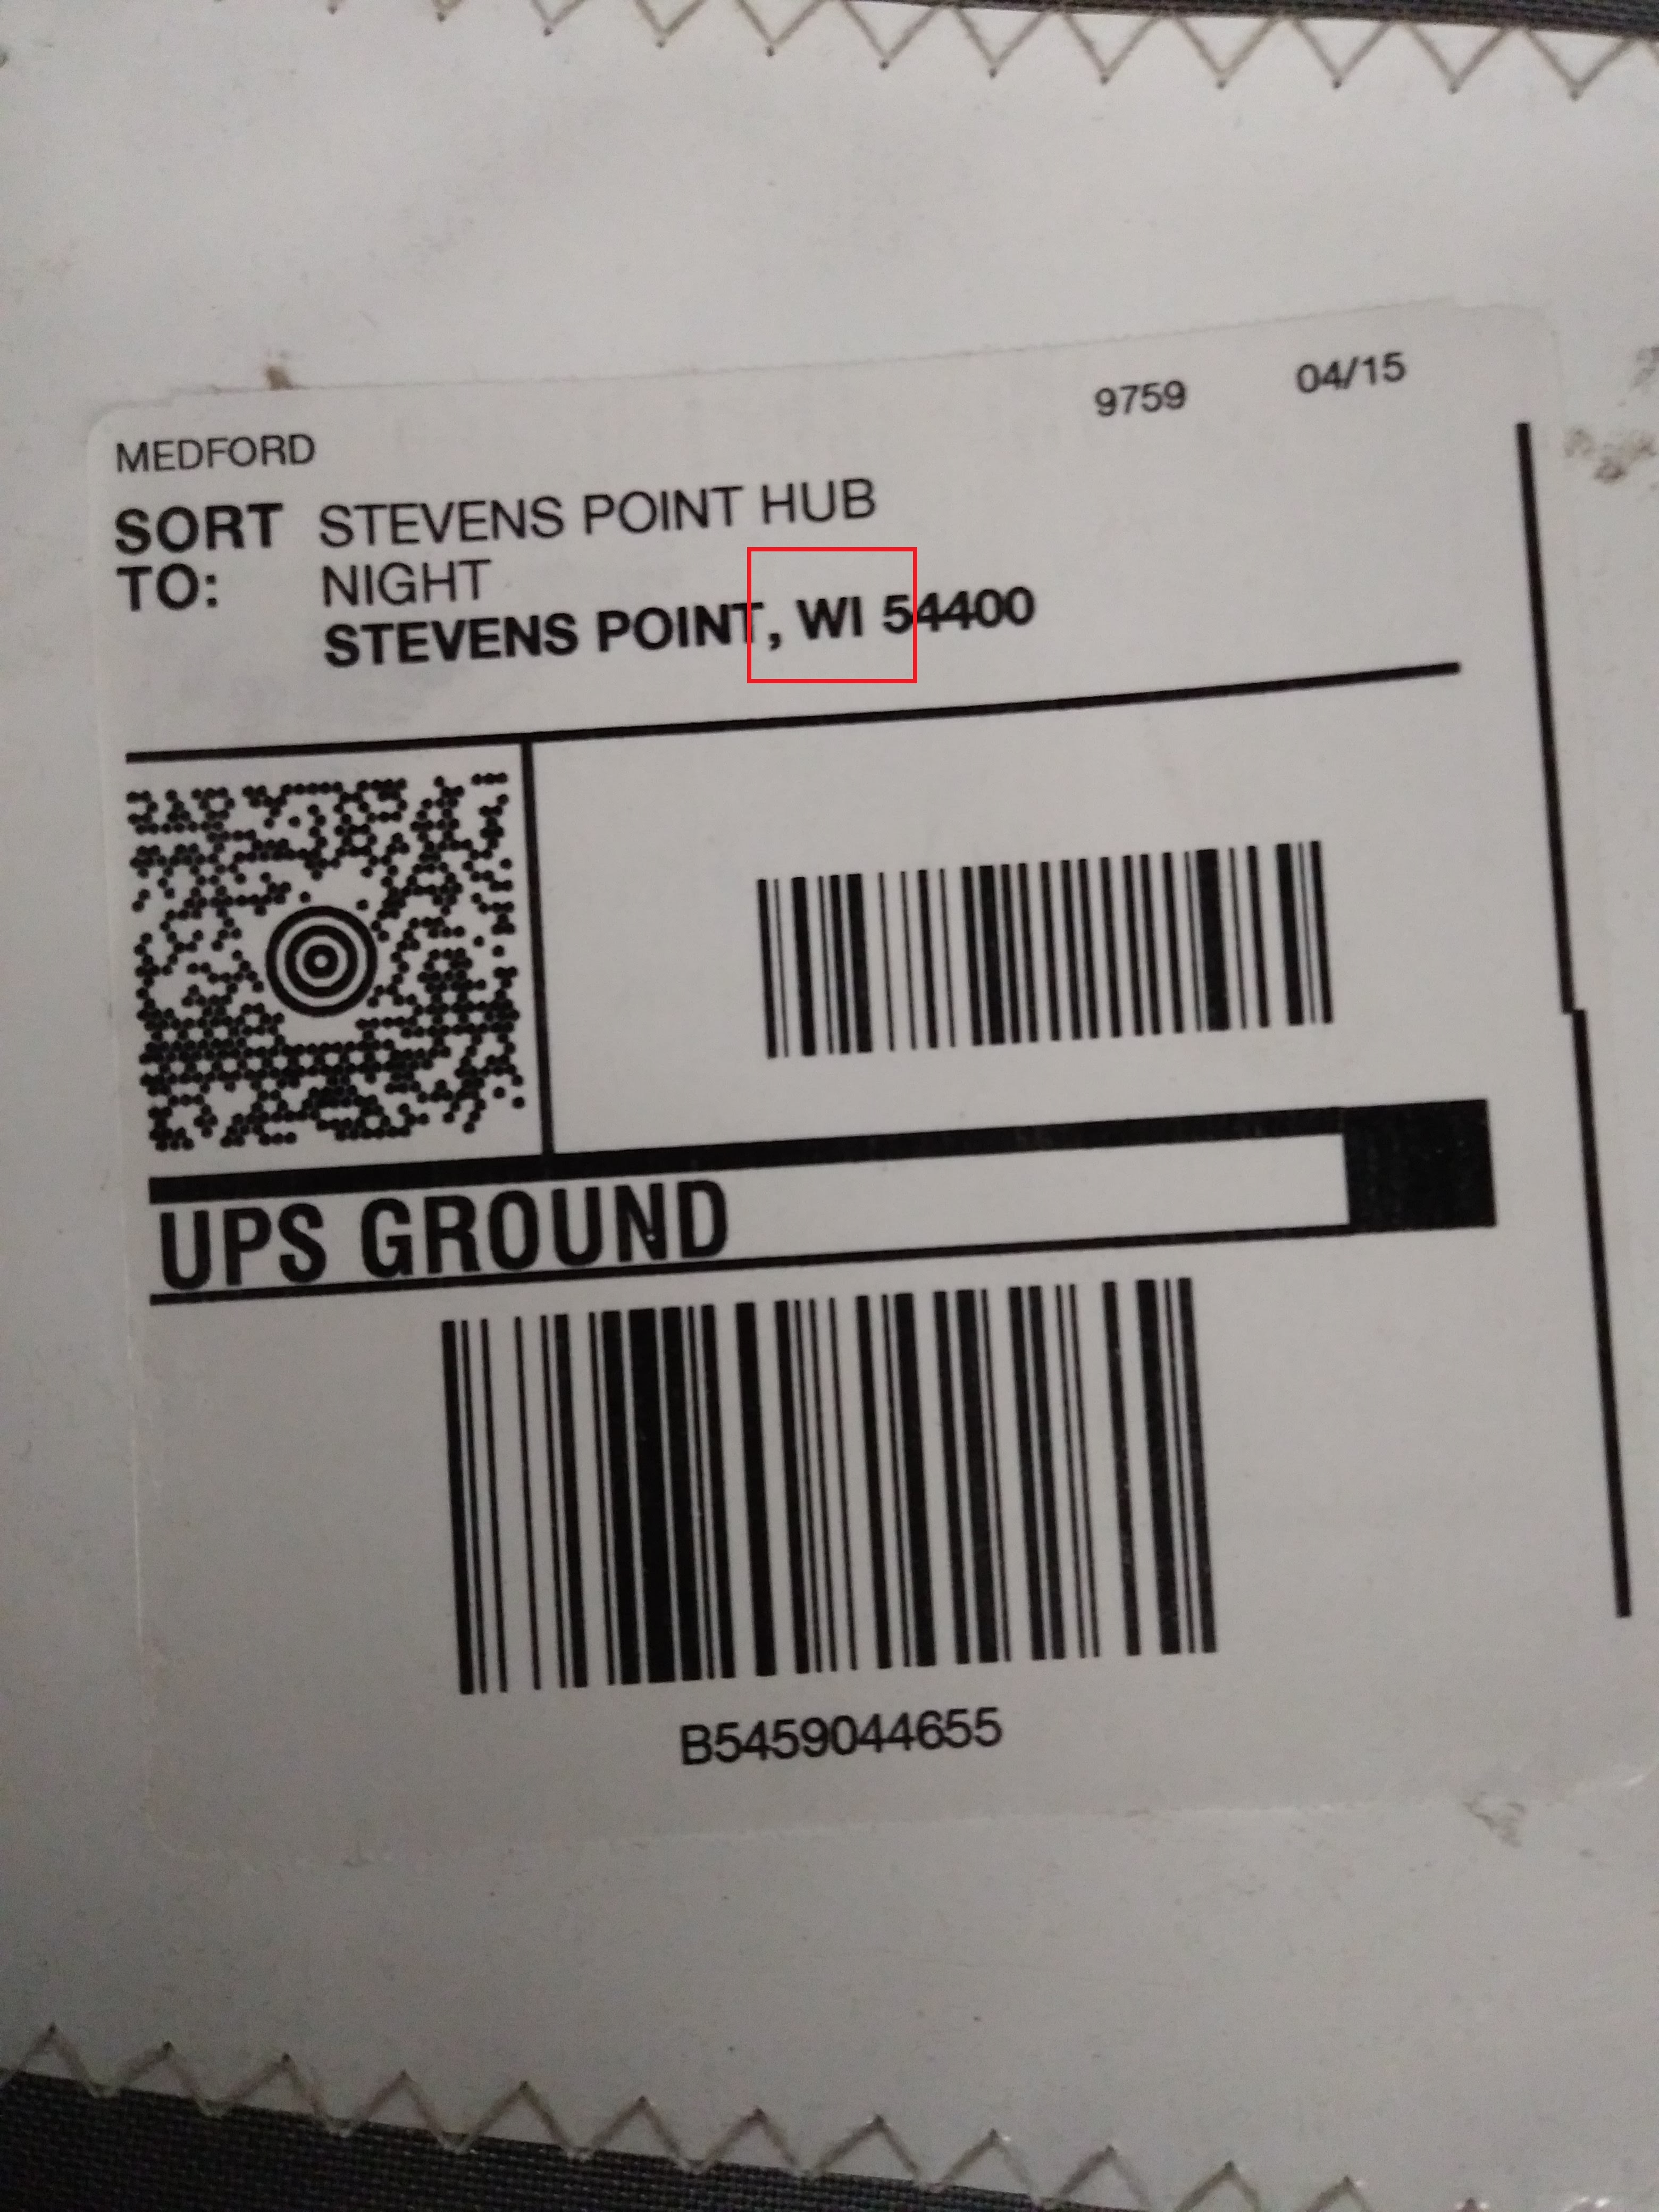
\includegraphics[width=0.5\linewidth]{20171221_161718}
\caption{Passthrough - No SLIC}
\end{subfigure}
\end{figure}
\clearpage
\subsection{Special Identification}

\subsubsection{Hazmat}
UPS often handles packages that contain hazardous materials. According to federal law, these boxes should be labeled accordingly. 

\begin{itemize}
    \item Hazmats cannot go to the small sort.
    \item If a hazmat packages begins to leak or expose material then evacuate the area.
    \item If you come in contact with a hazardous material then follow the appropriate cleanup and response measures immediately. Refer to MSDS on the box or with DNP if necessary.
\end{itemize}

\begin{figure}[H]
\begin{subfigure}{0.5\textwidth}
\centering
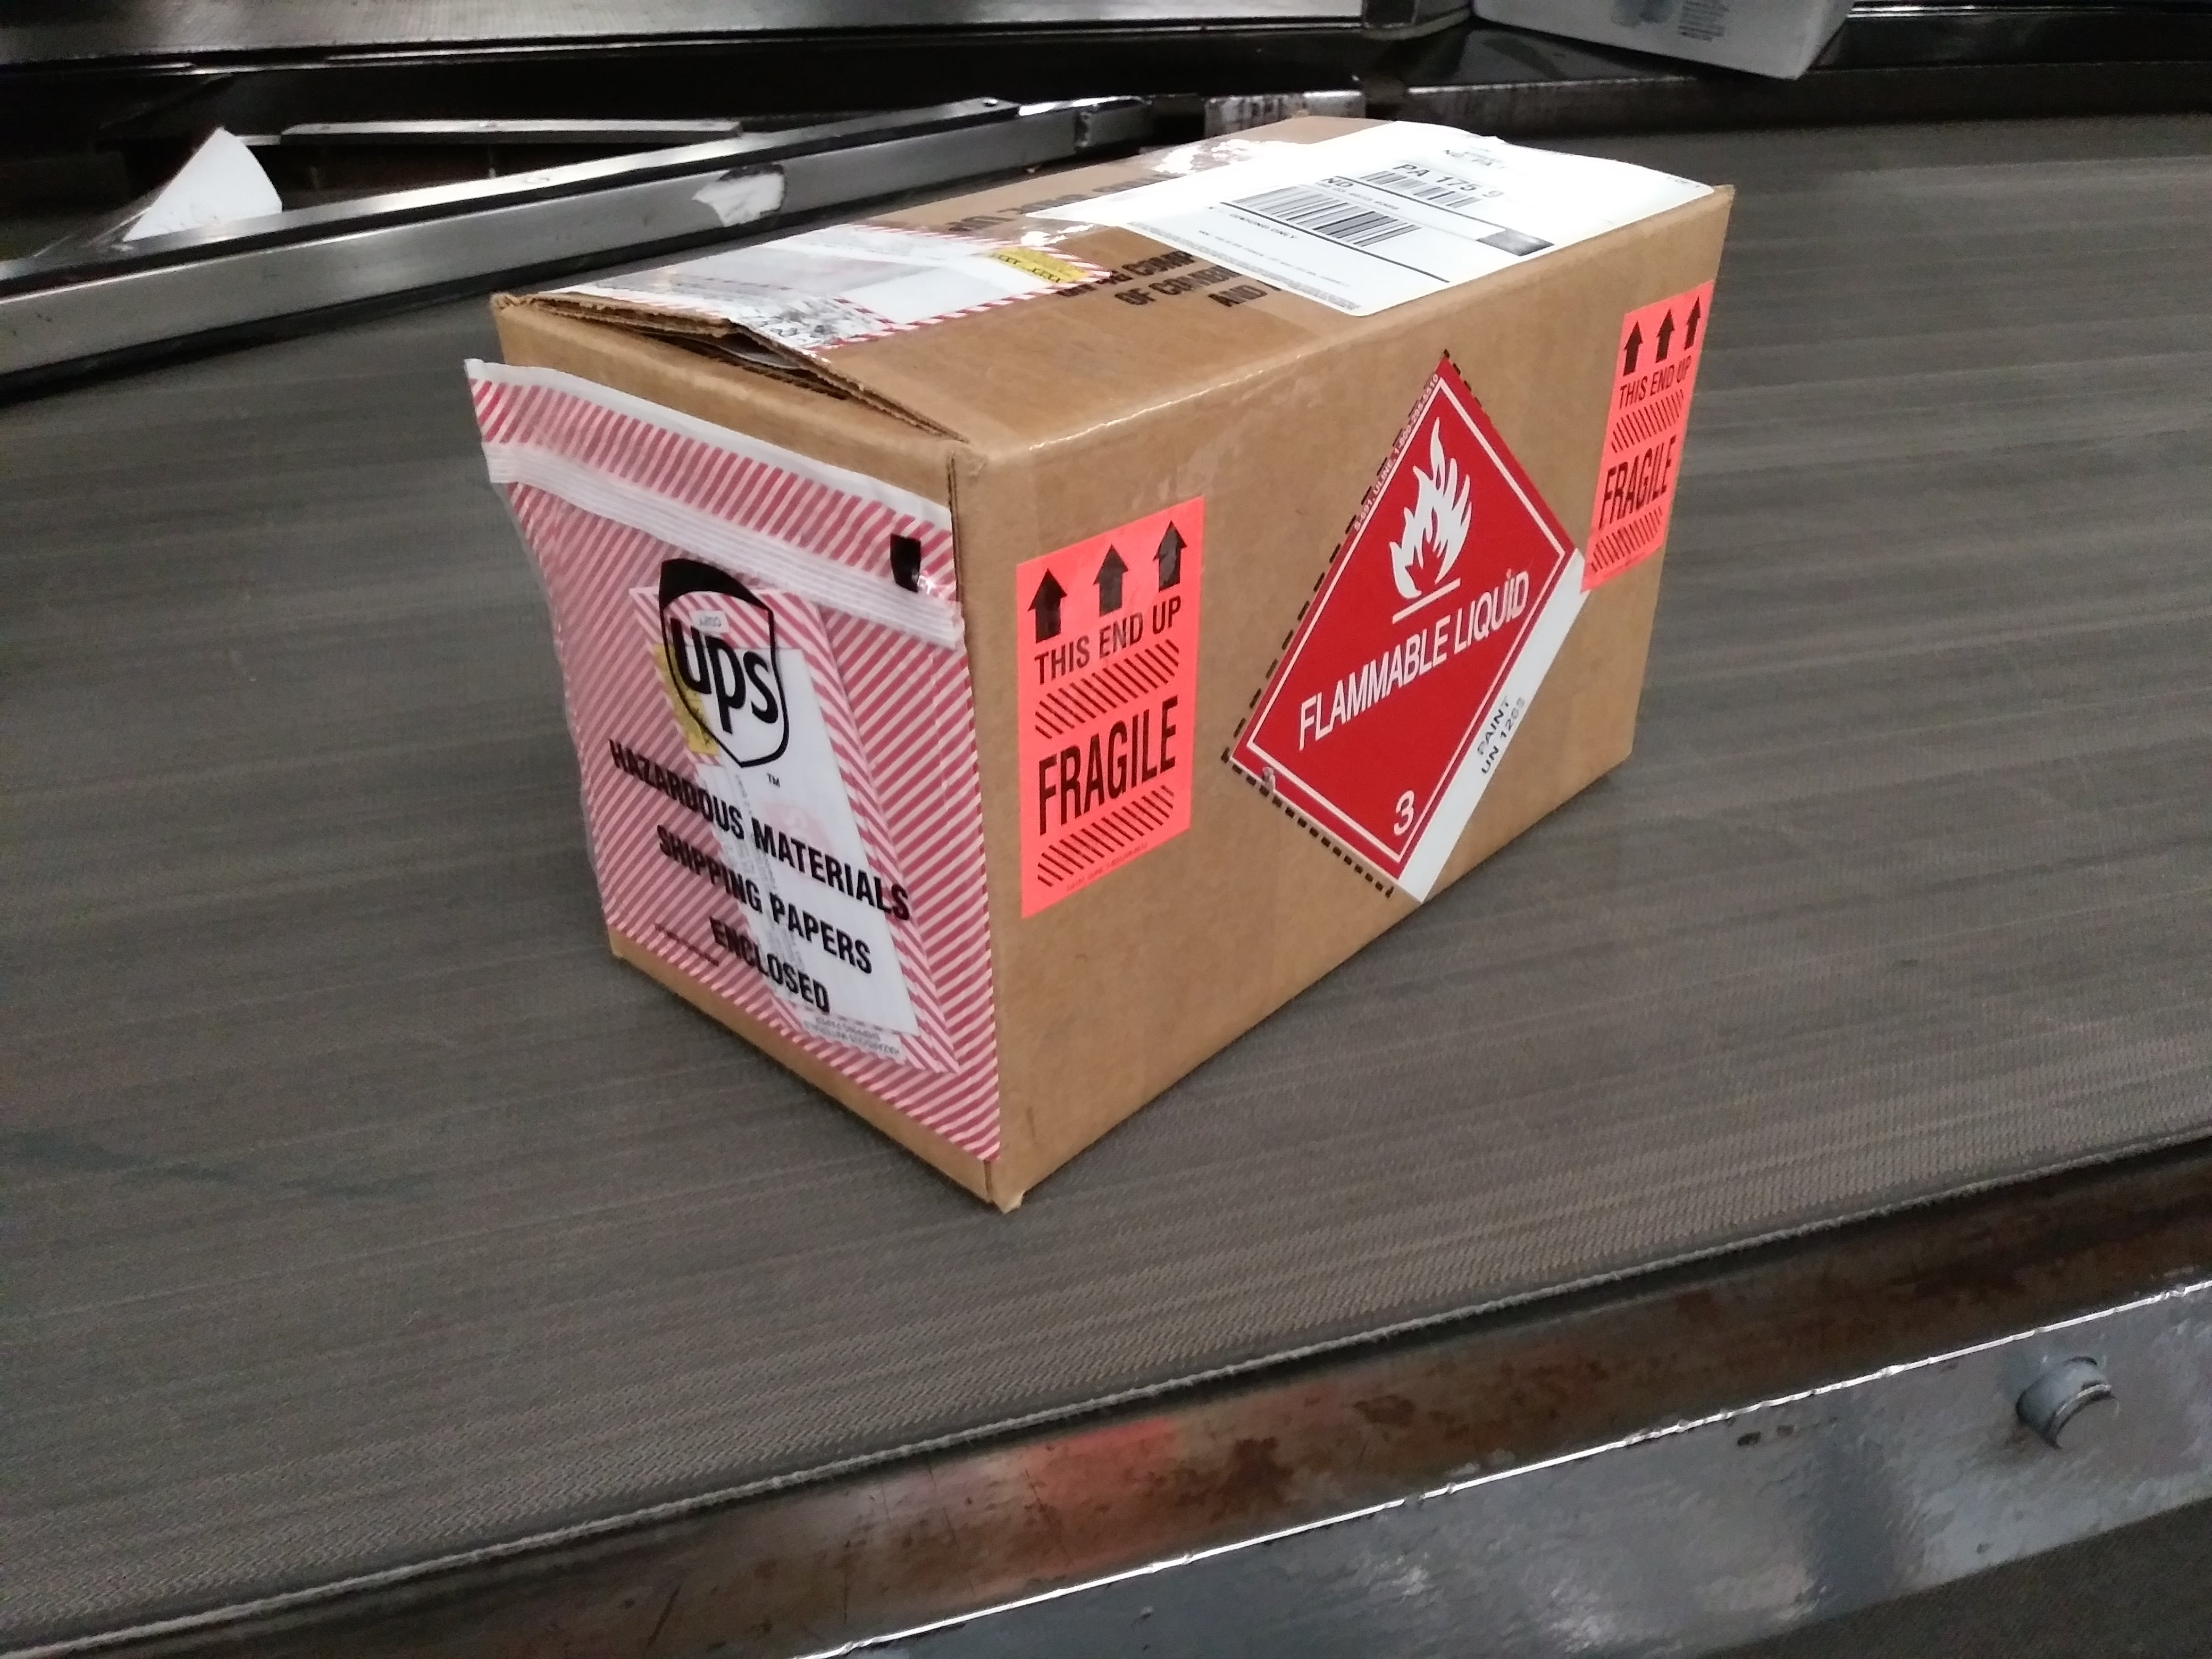
\includegraphics[width=0.7\linewidth]{20171221_183124} 
\caption{Flammable}
\end{subfigure}
\begin{subfigure}{0.5\textwidth}
\centering
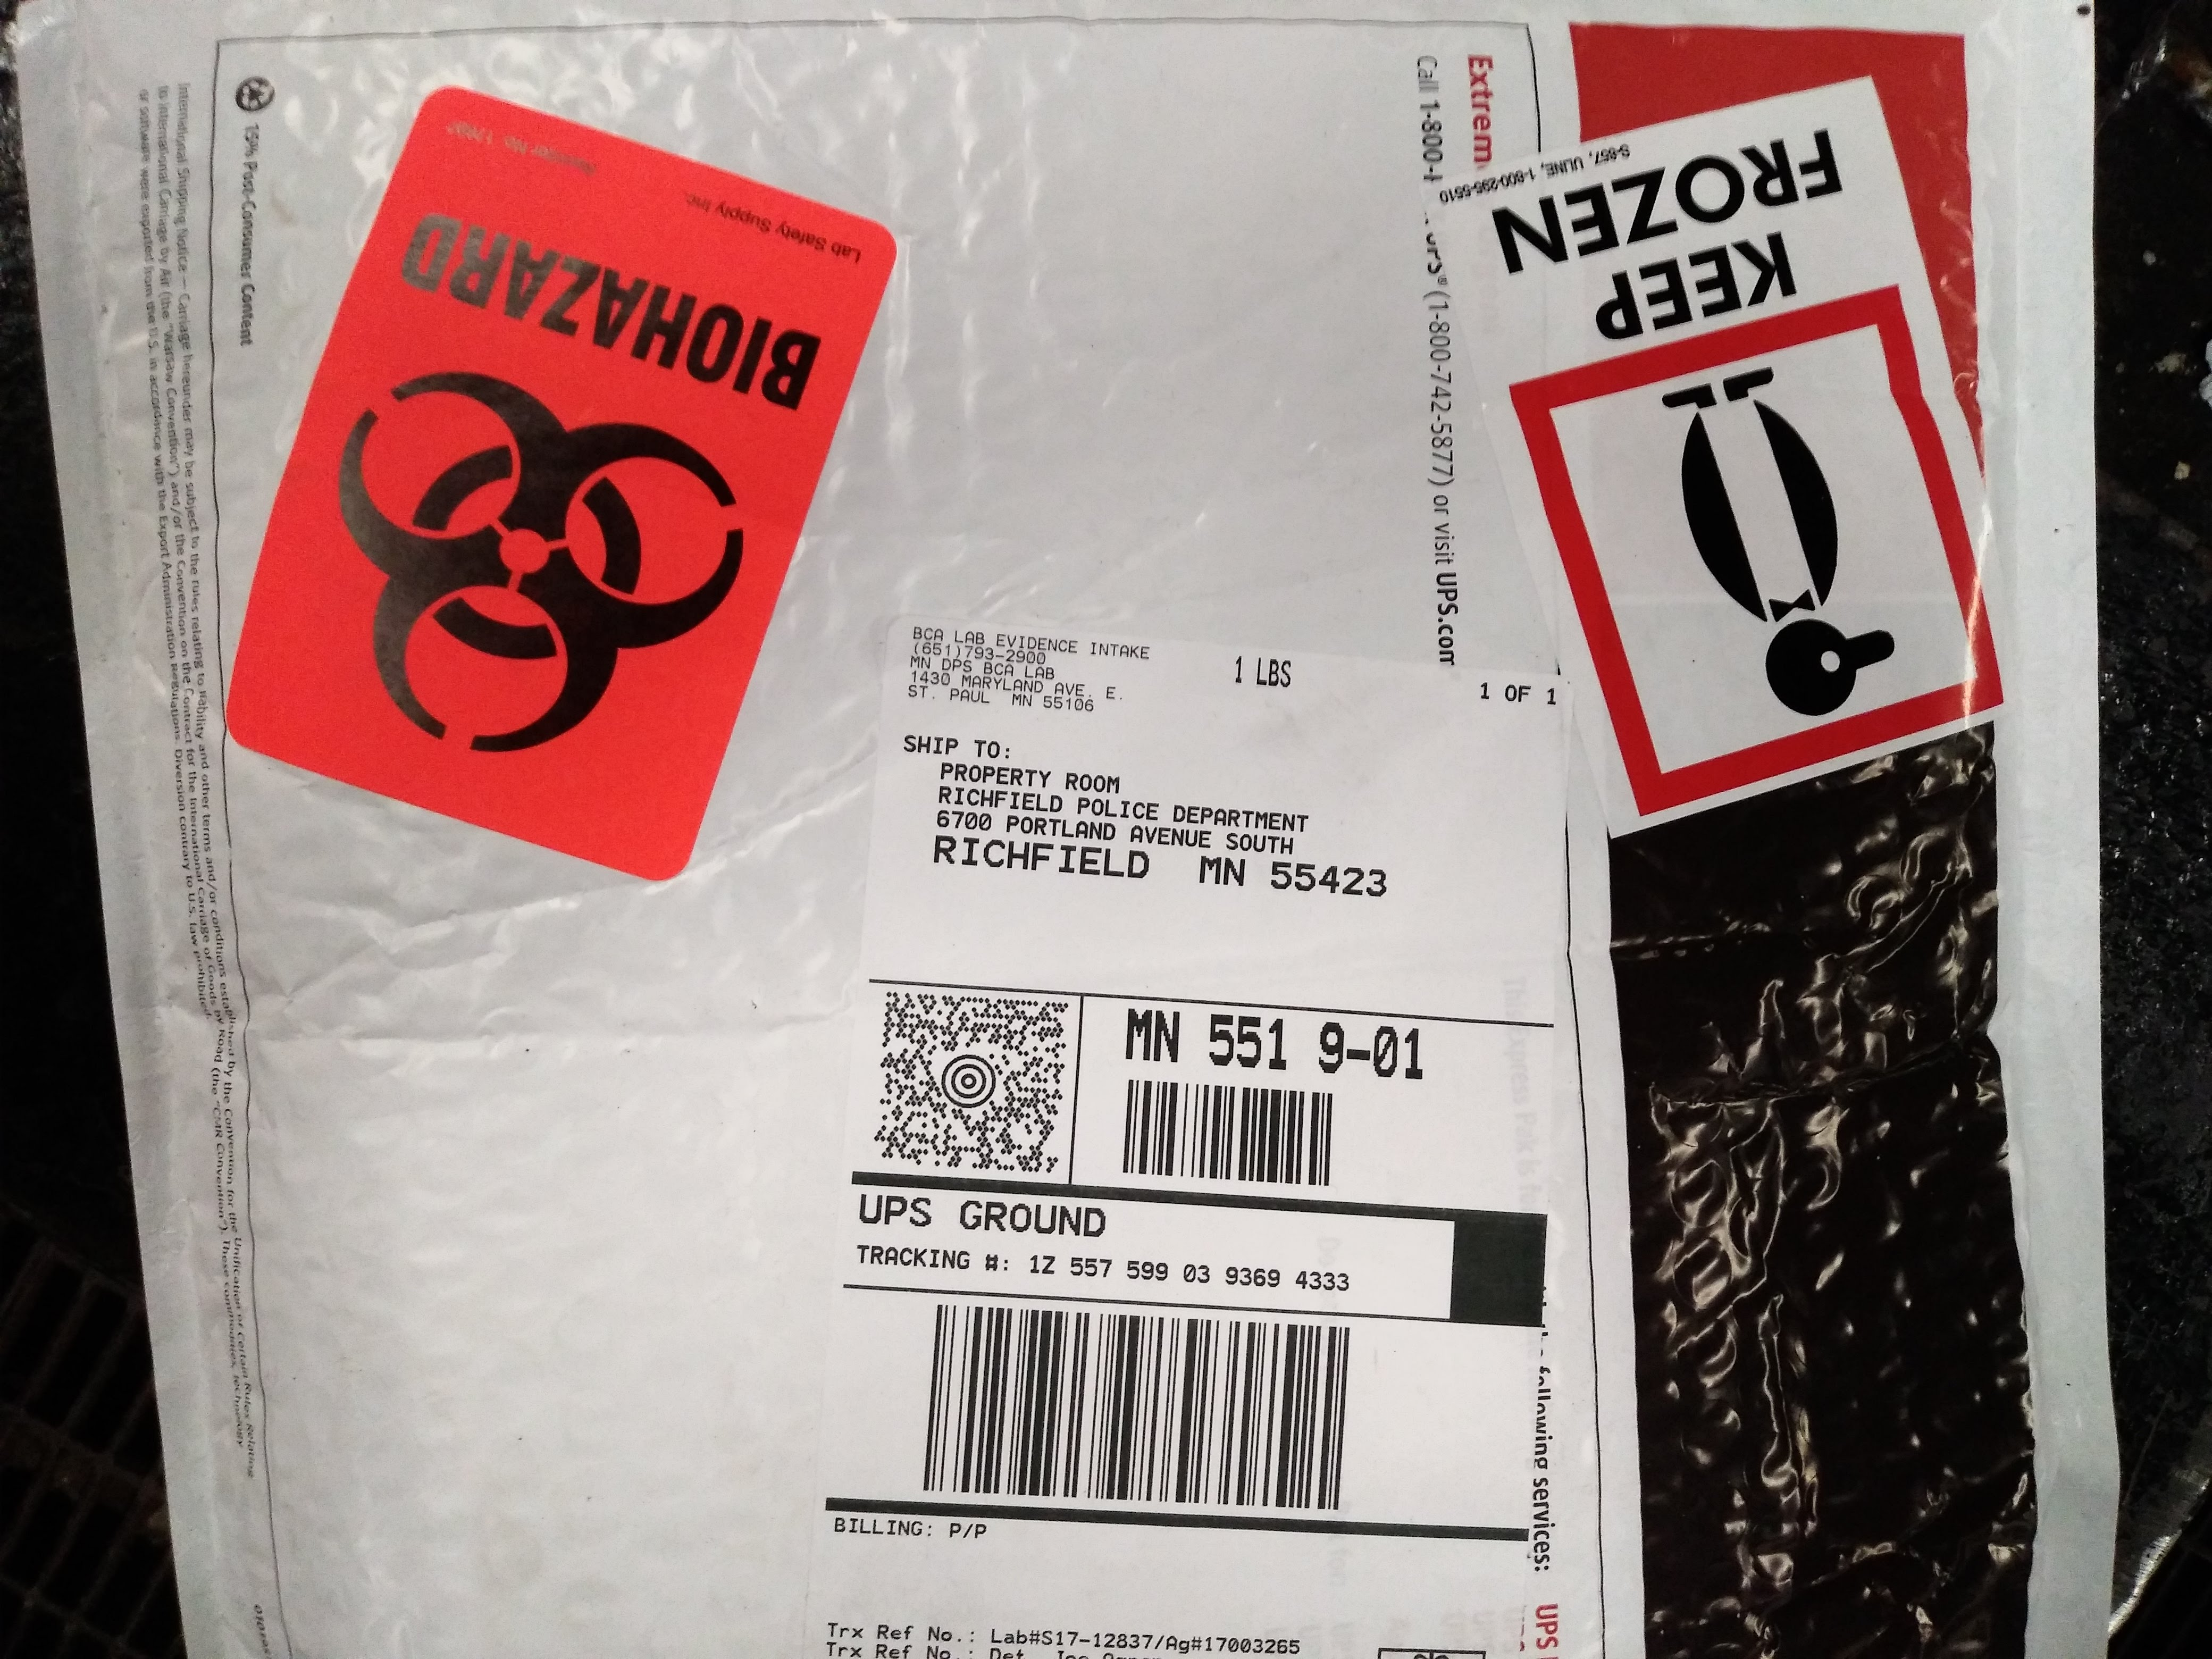
\includegraphics[width=0.7\linewidth]{20171221_191646}
\caption{Biohazard}
\end{subfigure}
\end{figure}

% \begin{figure}[h]

% \begin{subfigure}{0.5\textwidth}
% 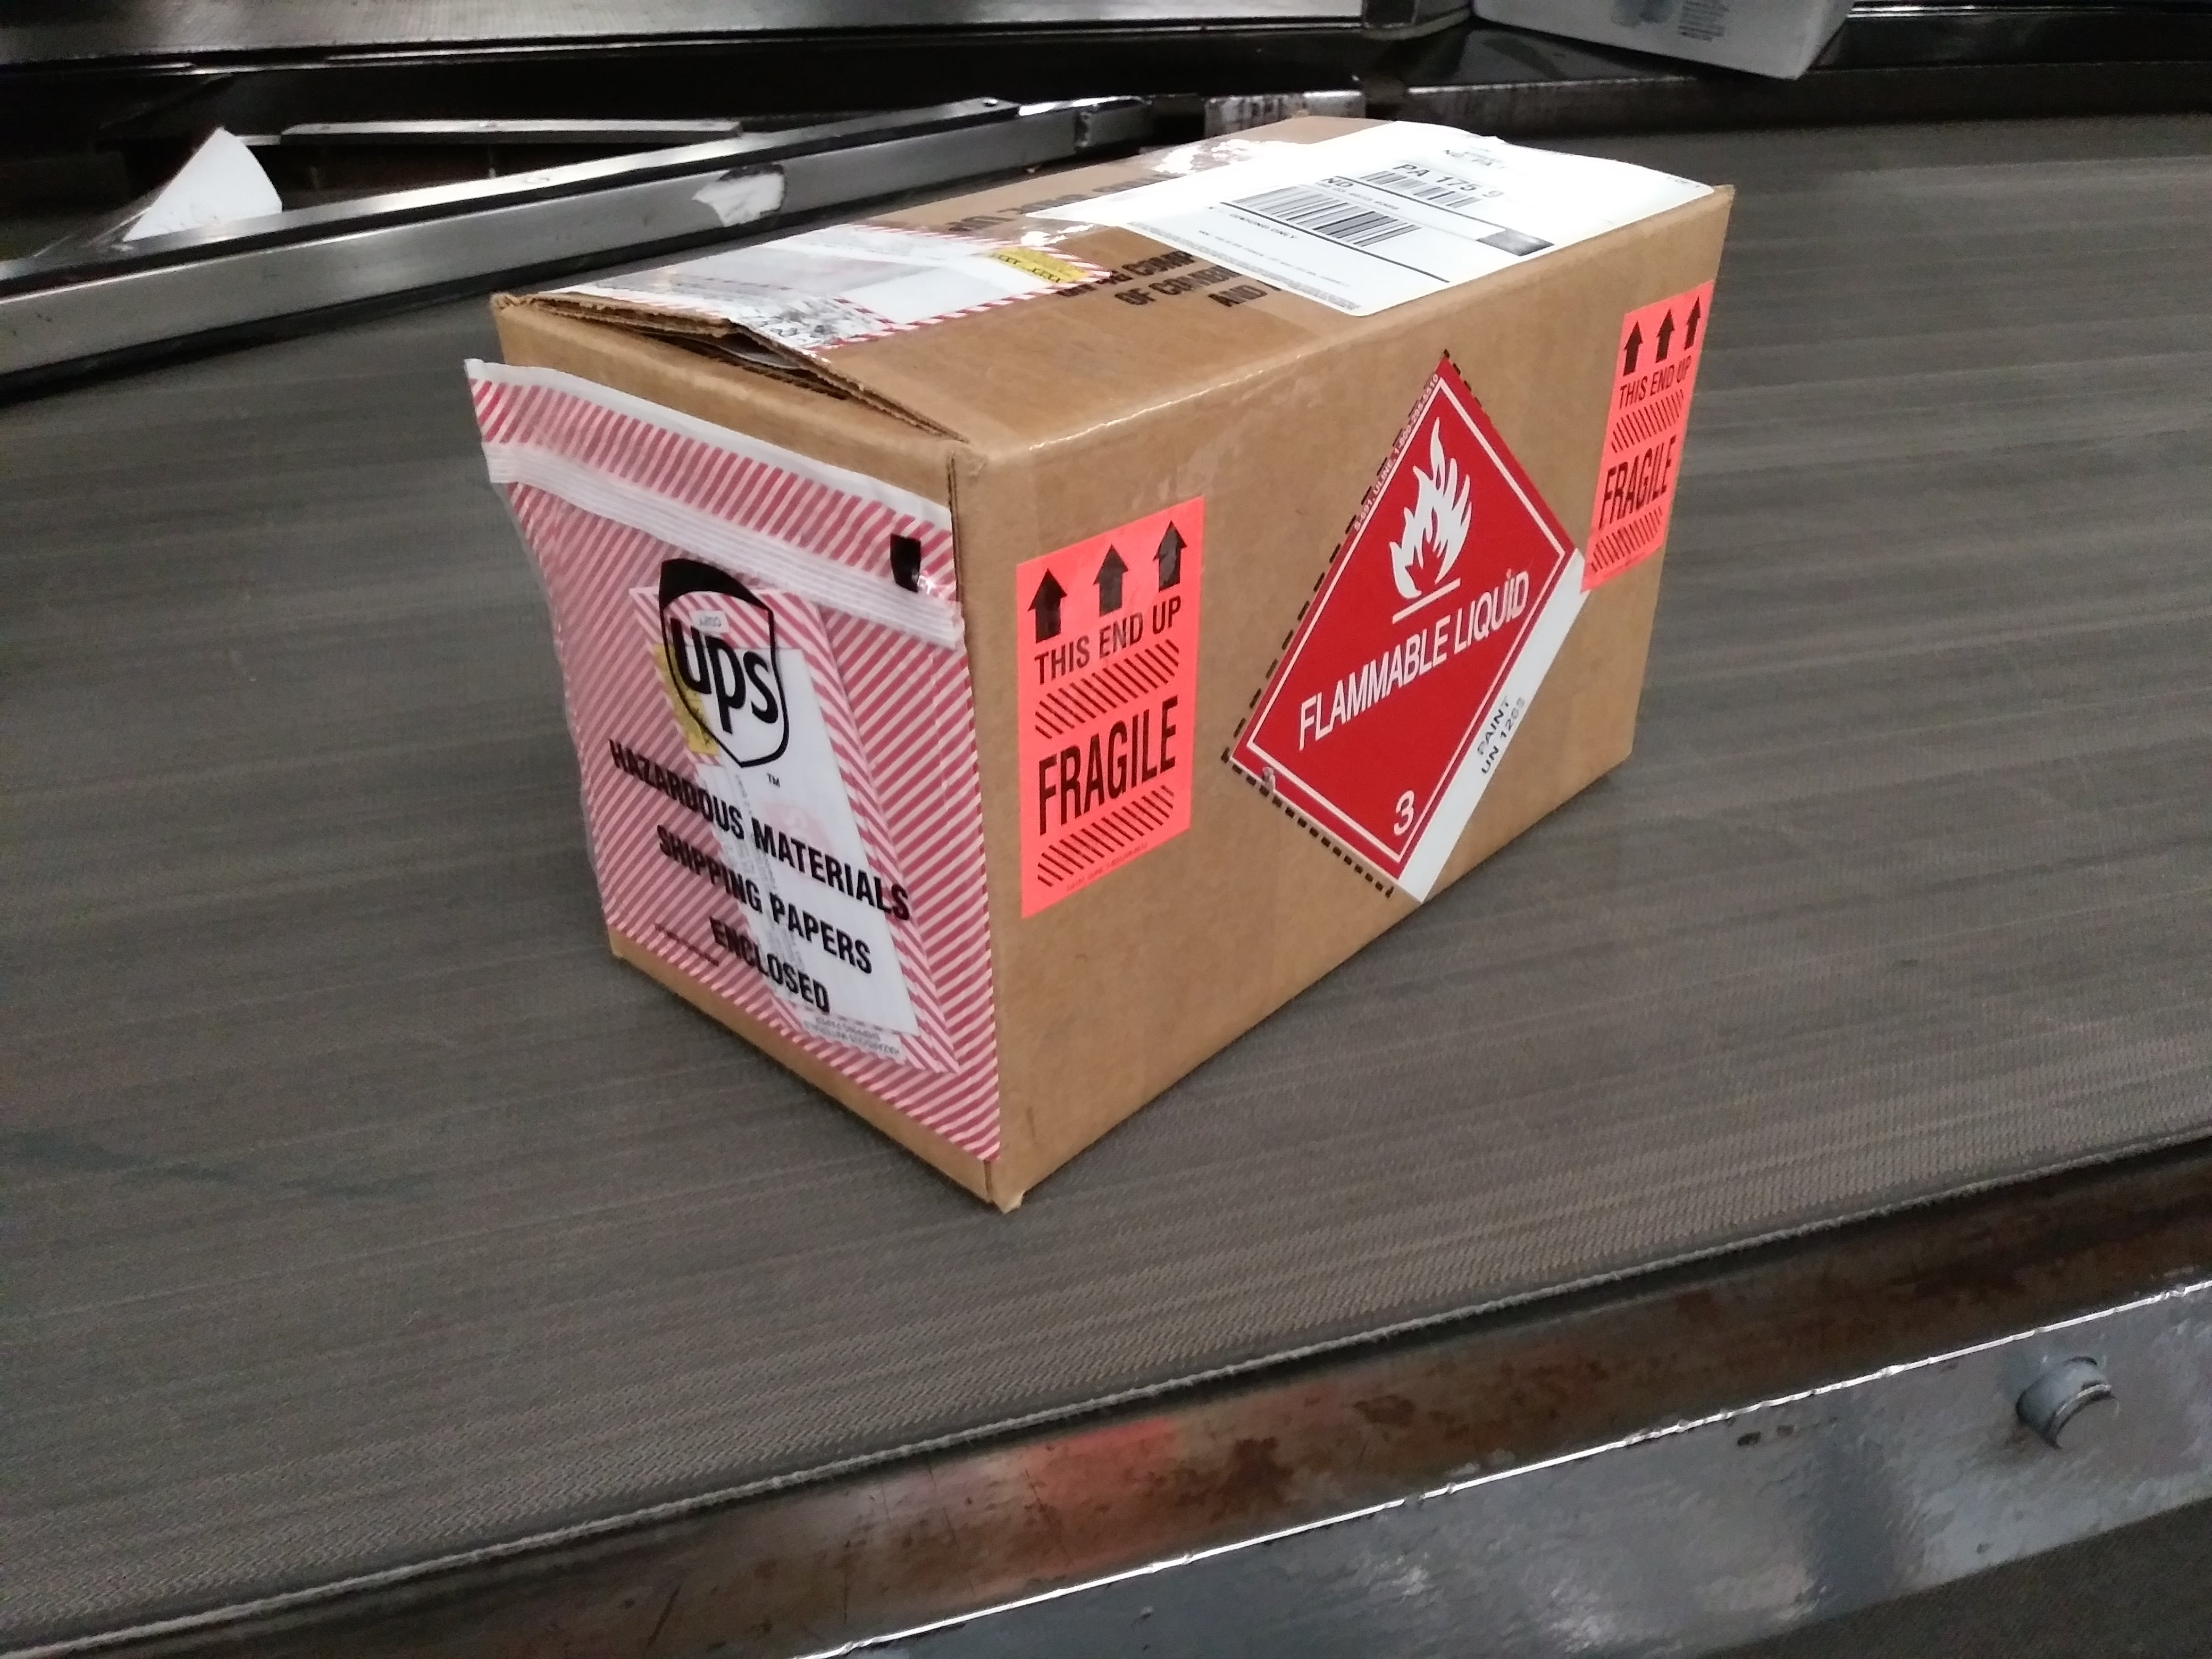
\includegraphics[width=0.4\linewidth, height=5cm]{20171221_183124} 
% \caption{Flammable}
% \end{subfigure}
% \begin{subfigure}{0.5\textwidth}
% 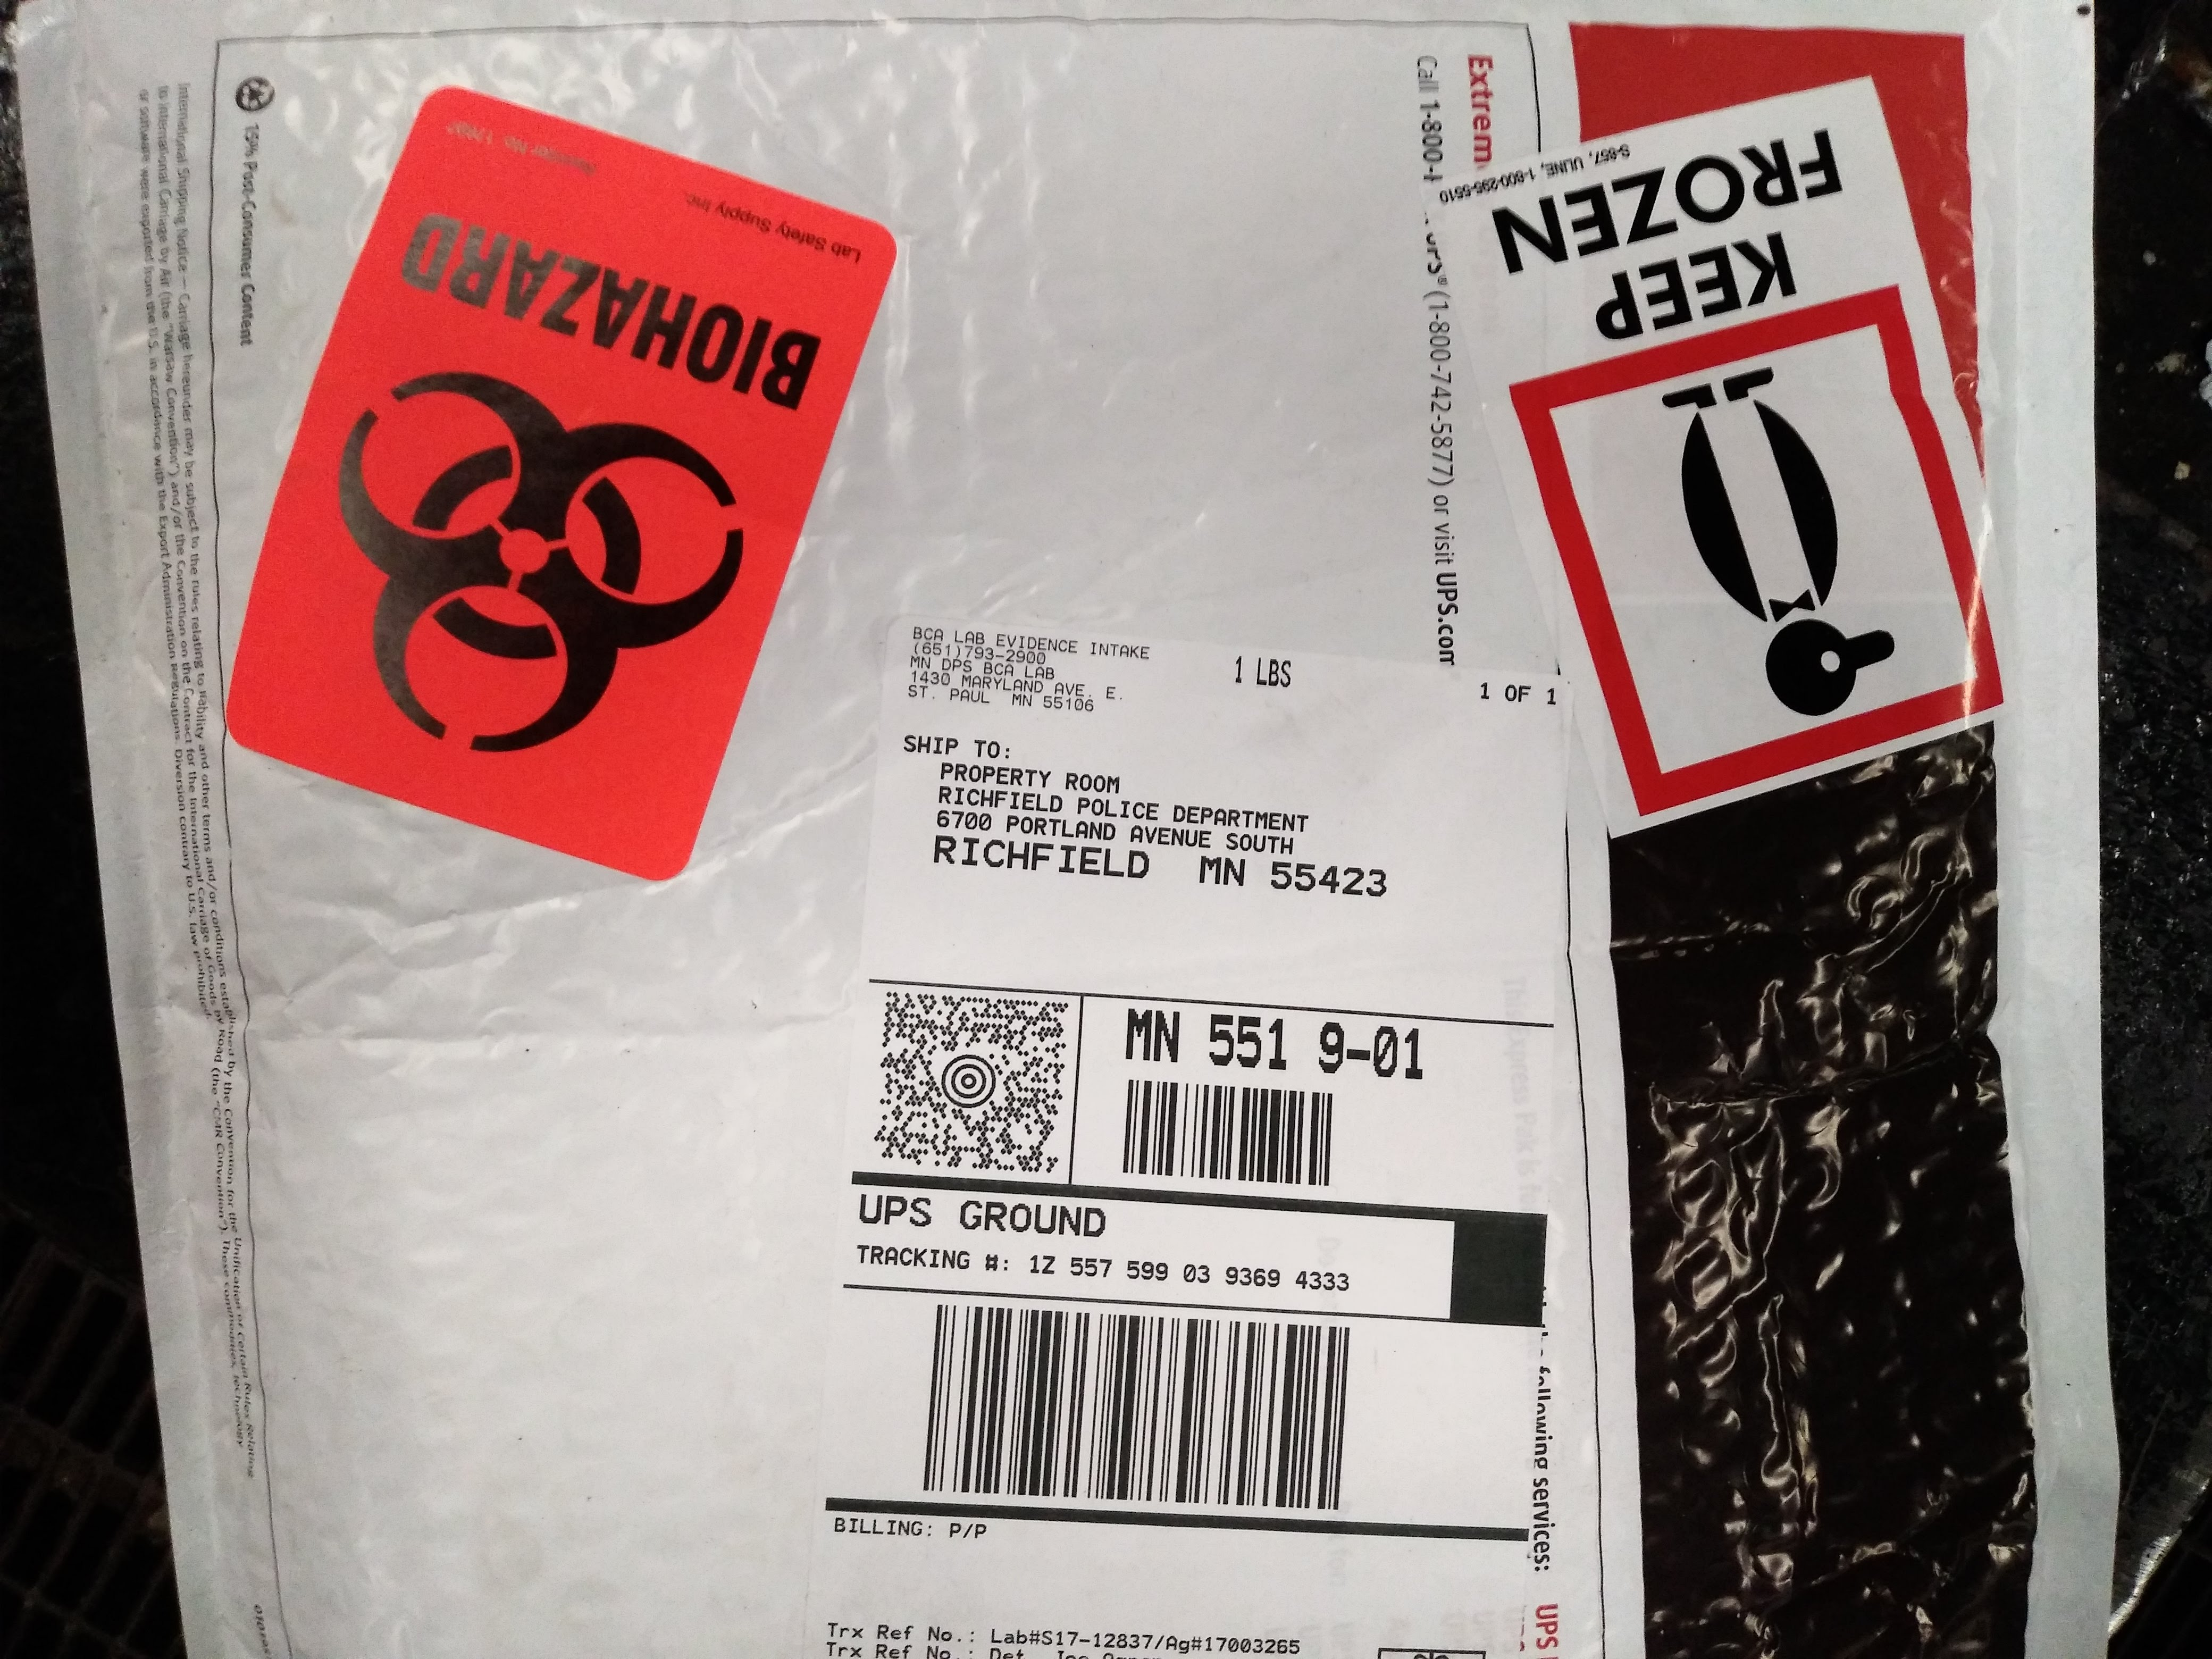
\includegraphics[width=0.4\linewidth, height=5cm]{20171221_191646}
% \caption{Biohazard}
% \end{subfigure}

% \end{figure}



% \subsubsection{Batteries}
% content



\subsubsection{ORM-D}
ORM-D stands for "other regulated materials for domestic transport only" and covers packages that present a real but limited hazard during transport. 

\begin{itemize}
    \item Since ORM-Ds are also hazmats, they cannot go to small sort.
\end{itemize}

\begin{figure}[H]
    \centering
    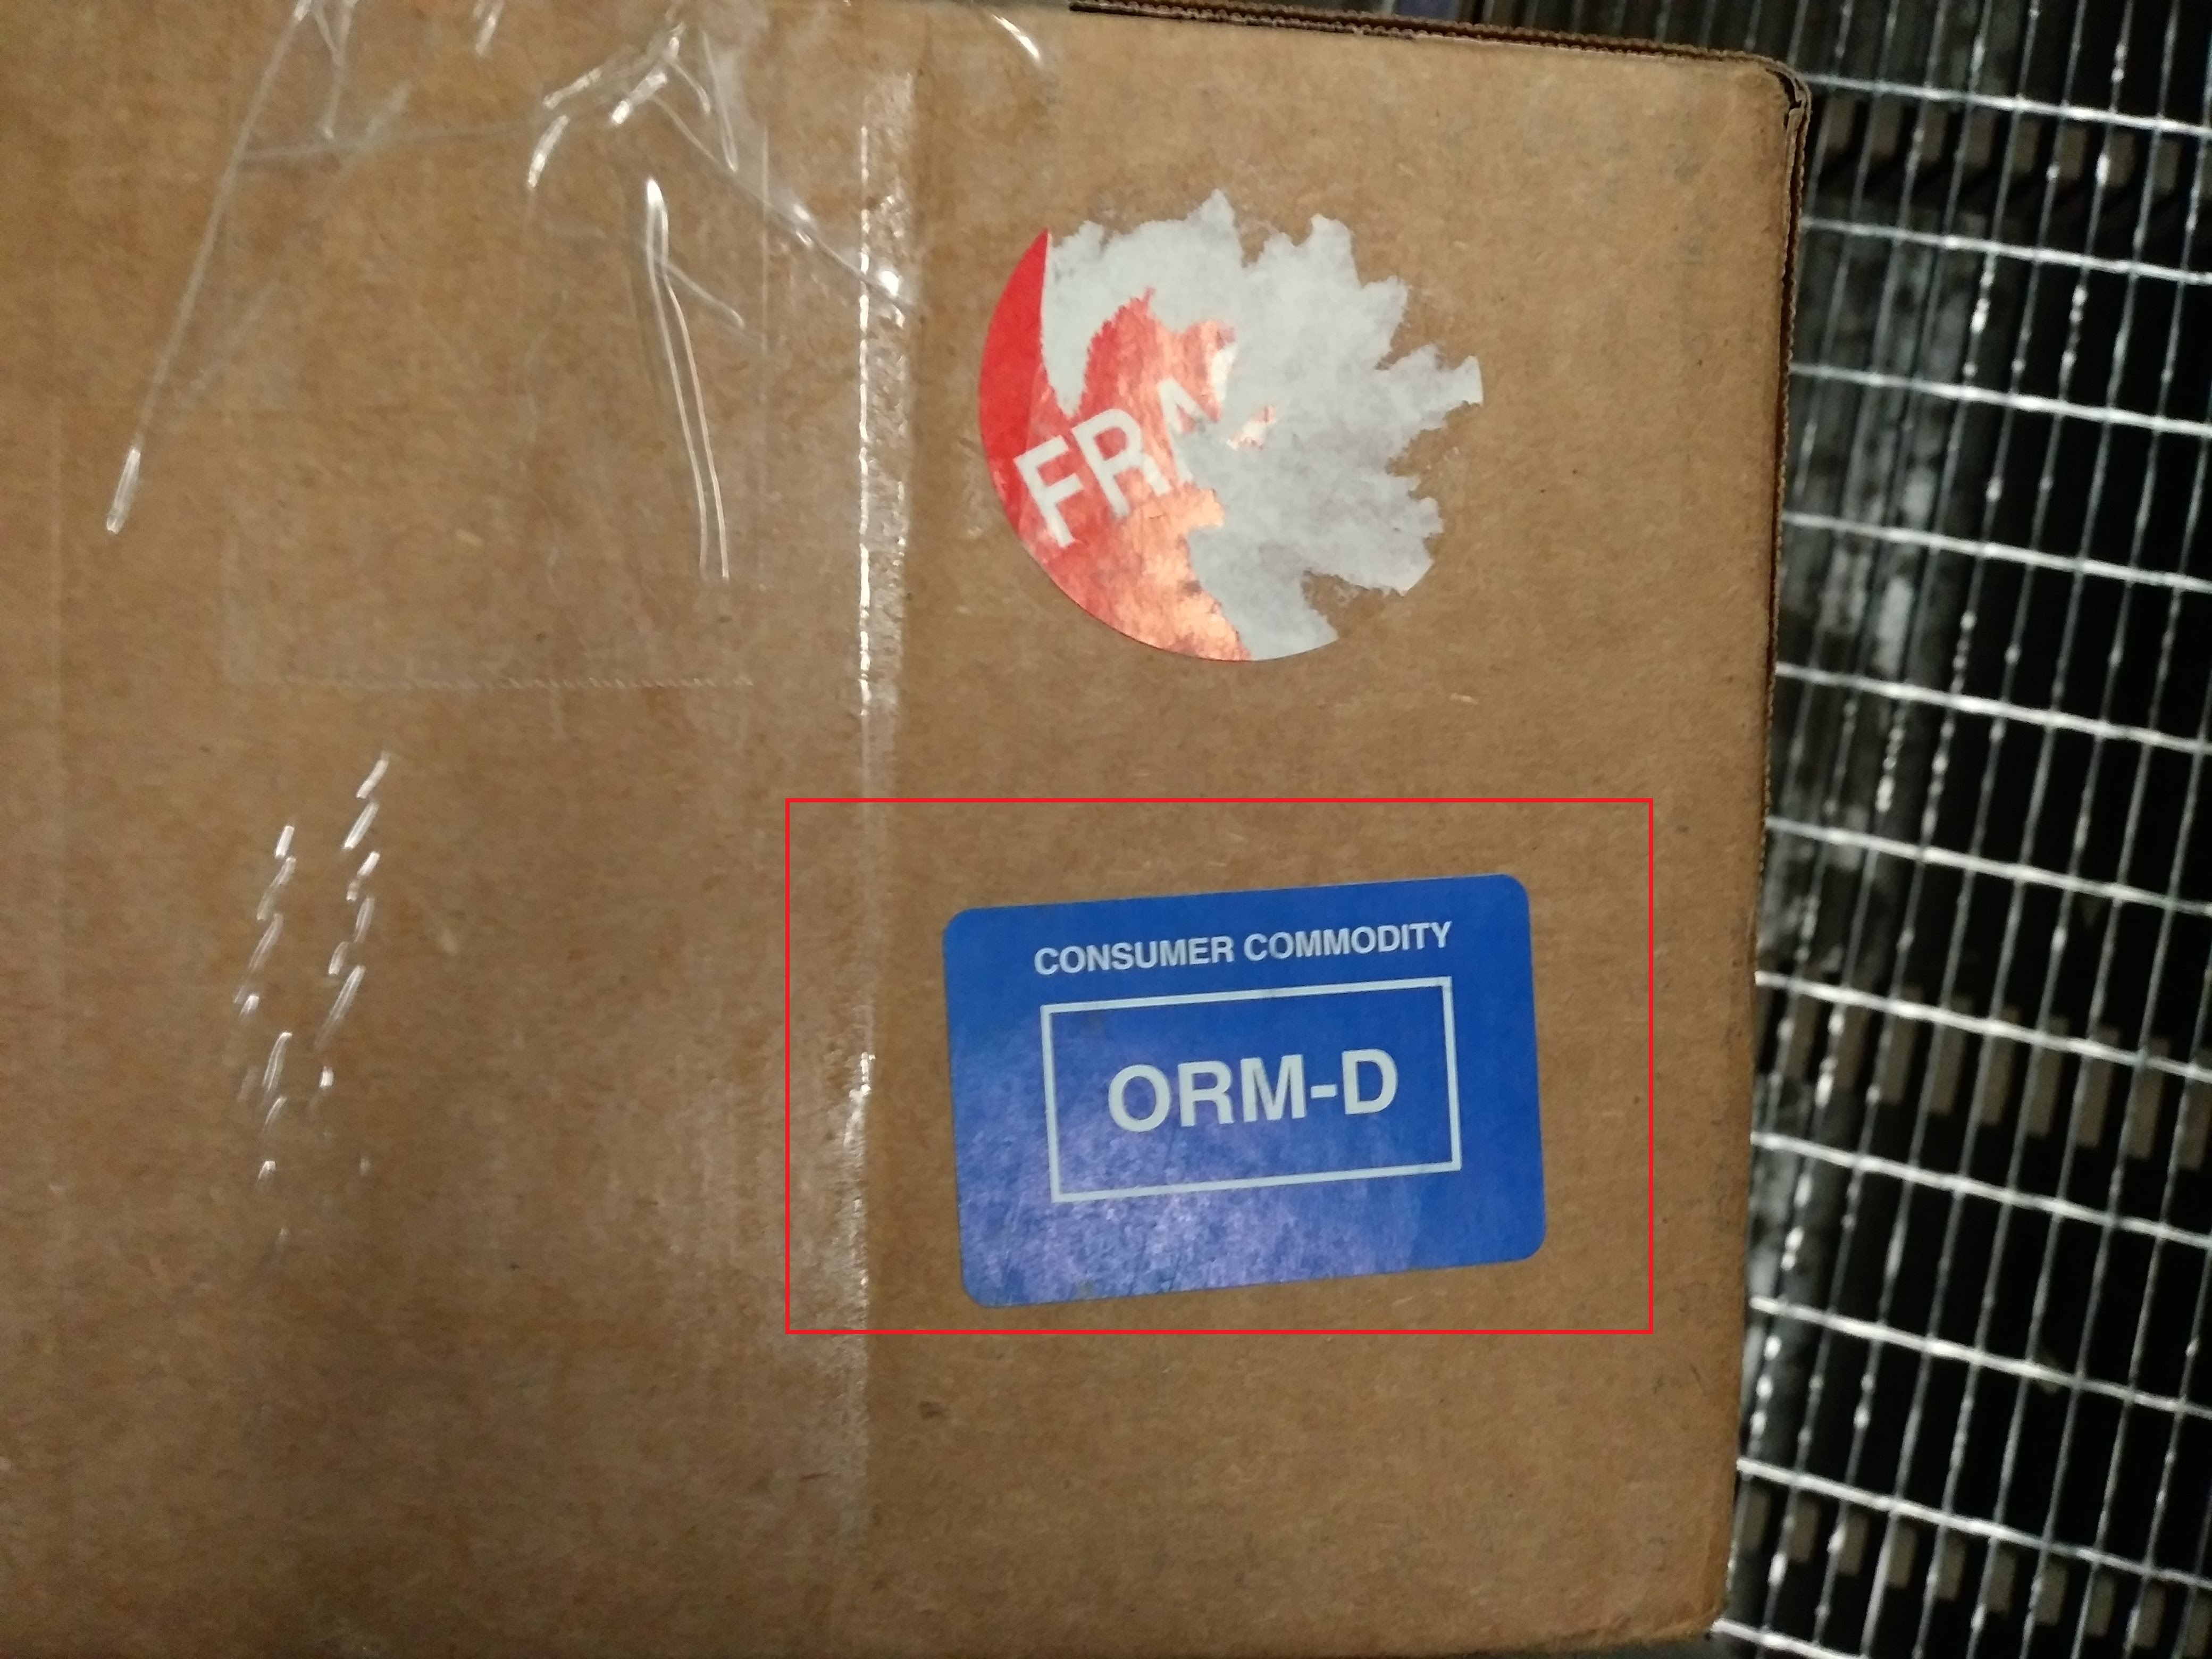
\includegraphics[width=0.4\linewidth]{20171221_171456}
    \caption{ORM-D Sticker}
\end{figure}

\subsubsection{High Value}
These are high value packages and are processed through a separate, dedicated department. Normally, unloaders are tasked with removing these from loads like an irreg, but they can be missed and end up on the sort aisle.

\begin{itemize}
    \item All high value bags that arrive at the sort aisle should be set aside to be delivered to the high value department.
\end{itemize}

\begin{figure}[H]
    \centering
    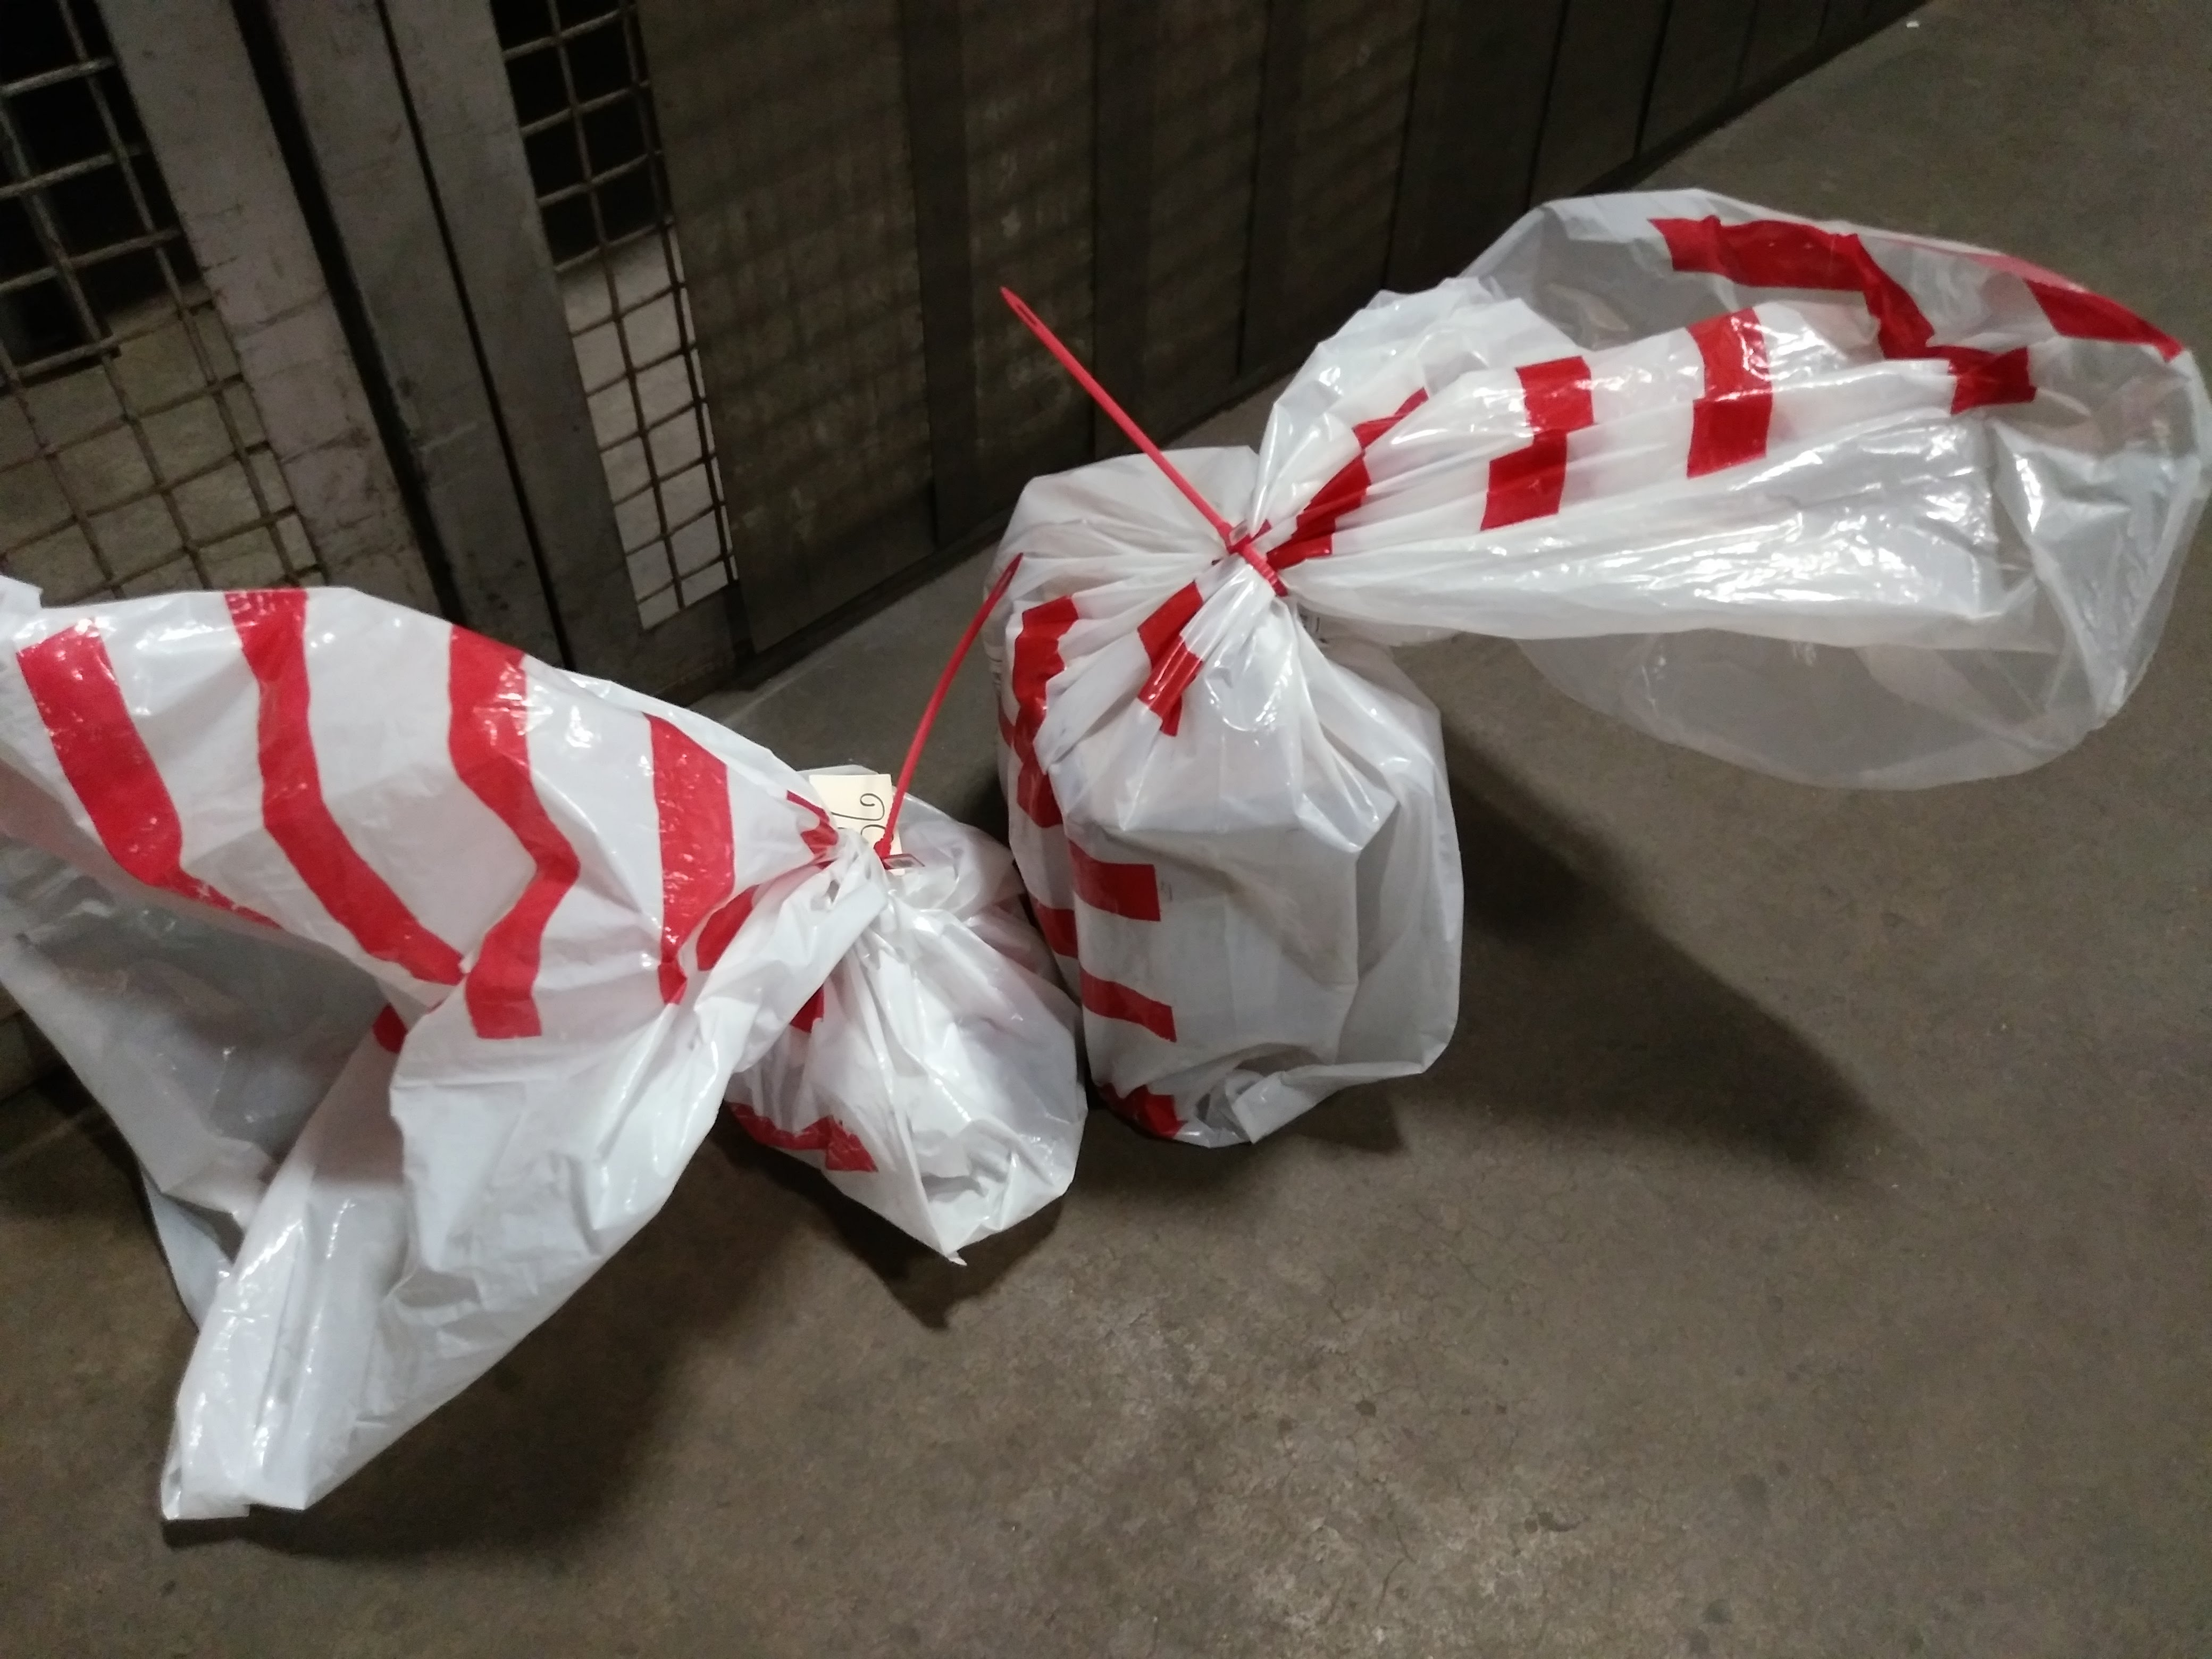
\includegraphics[width=0.4\linewidth]{20171222_022332}
    \caption{High value bags}
\end{figure}

\subsubsection{Wrong Carrier}
In some cases, UPS will end up with other carrier's volume. This is normal, and UPS has a process to deal with it.

\begin{itemize}
    \item Determine that the package does not have a UPS label.
    \item If the package is clearly intended for another carrier then set it aside for a supervisor to bring to the USPS/FedEx drop off.
\end{itemize}

\begin{figure}[H]
\begin{subfigure}{0.5\textwidth}
\centering
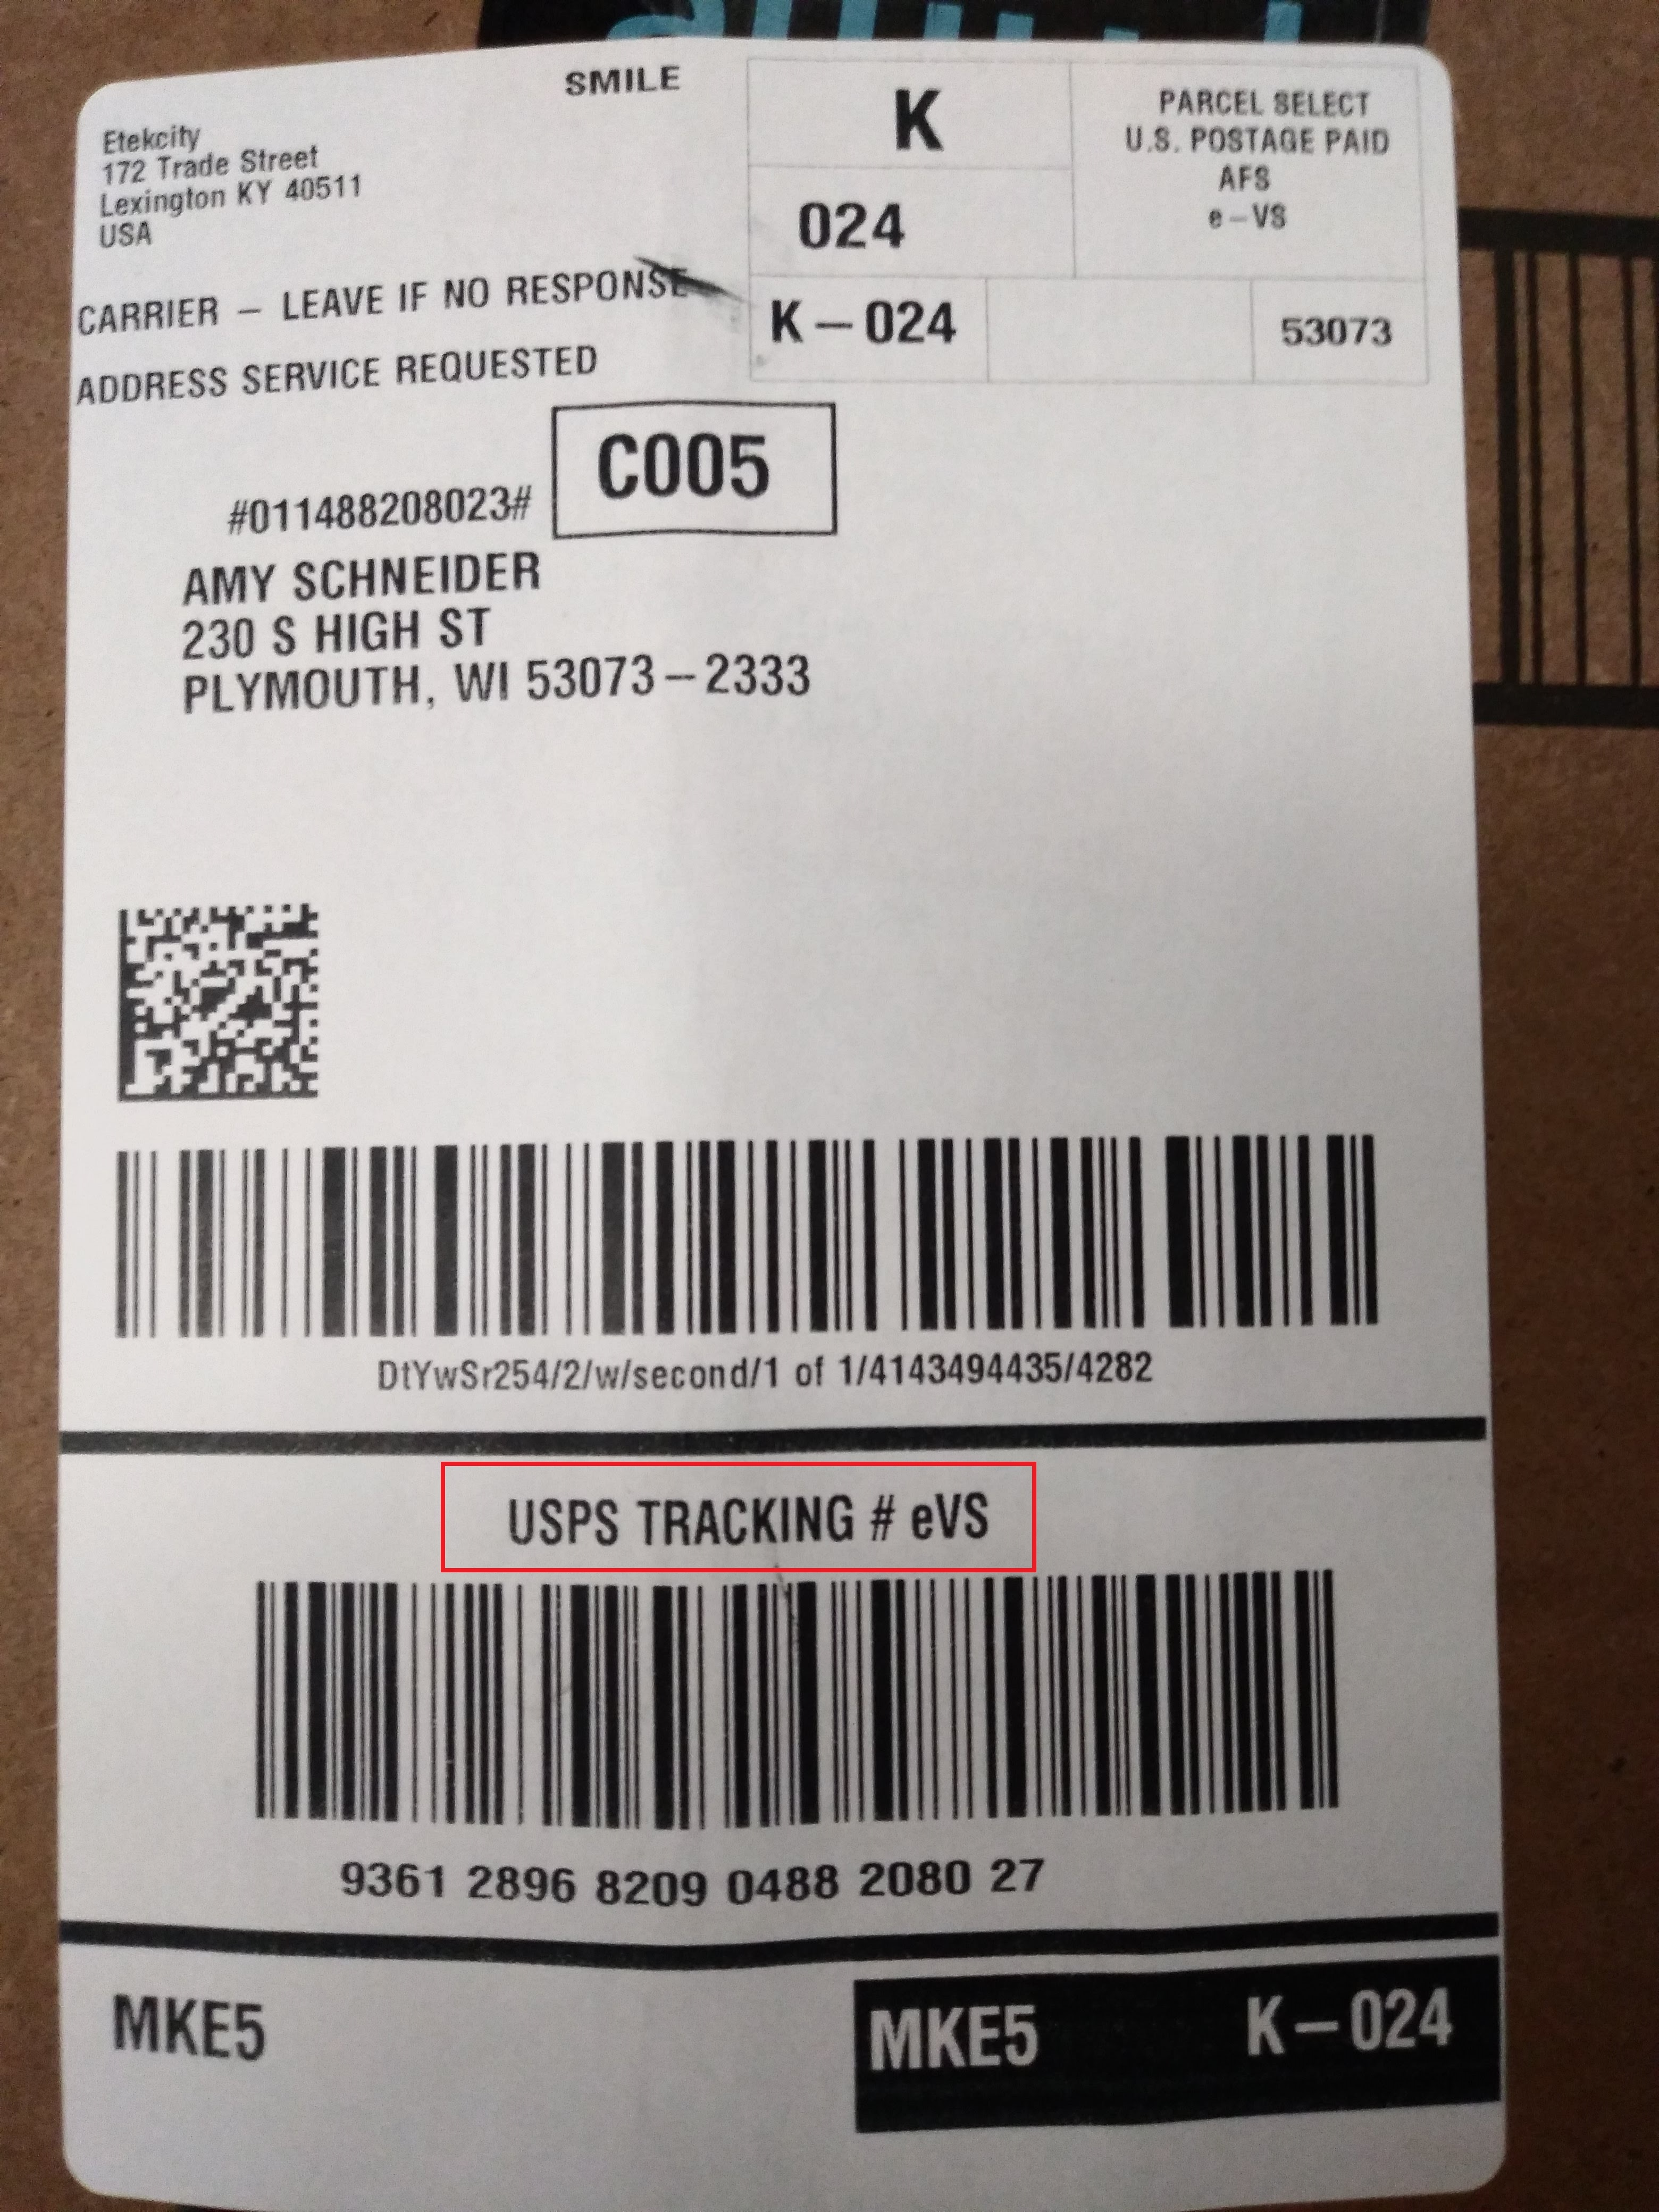
\includegraphics[angle=90,width=0.7\linewidth]{20171221_153203}
\caption{USPS}
\end{subfigure}
\begin{subfigure}{0.5\textwidth}
\centering
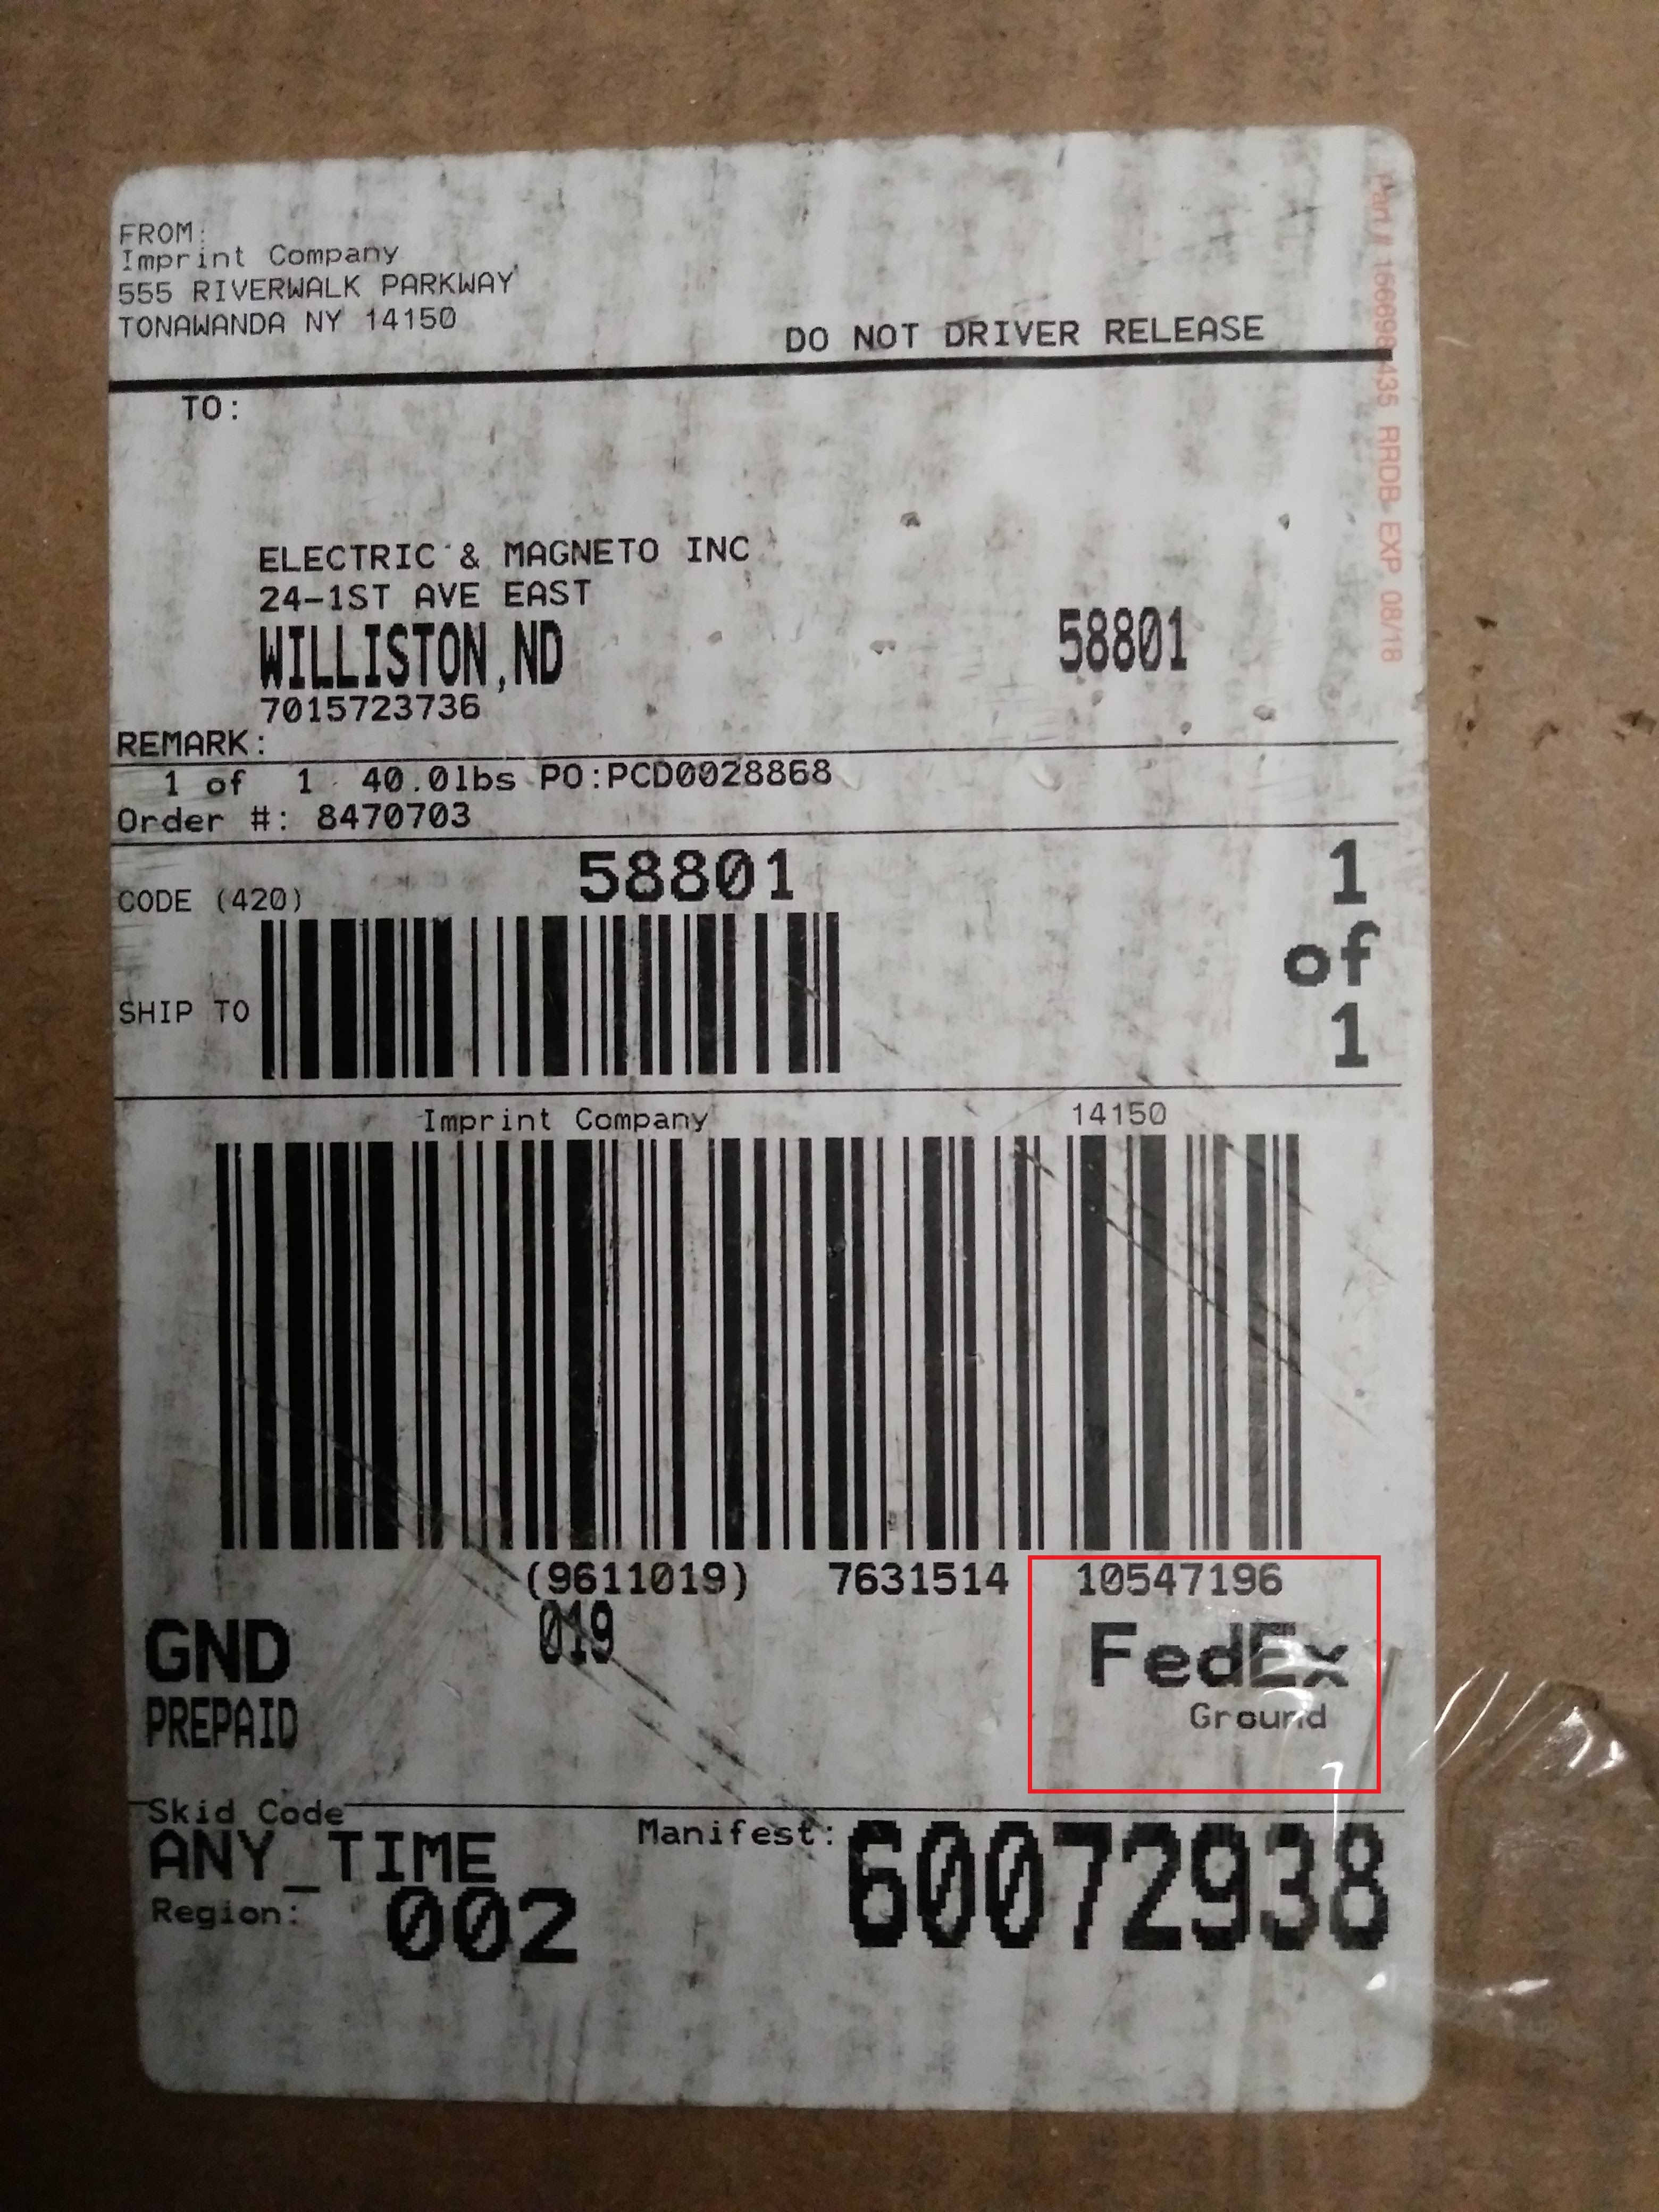
\includegraphics[angle=90,width=0.7\linewidth]{20171221_183158}
\caption{FedEx}
\end{subfigure}
\end{figure}

\subsubsection{Canada}
Given MN's norther location, we can end up handling a great deal of Canadian volume. While these are processed normally by following the International table, there are some extra considerations. Every Canadian package will have to cross an international border at some point and needs to be audited as a result. Whether a package has been audited is indicated by a green "ODC" sticker.

\begin{itemize}
    \item All Canadian packages must carry an ODC sticker.
    \item Any package missing the ODC sticker must be sent to the blue belt.
    \item Do no send any Canadian package to small sort without an ODC sticker.
\end{itemize}

\begin{figure}[H]
    \centering
    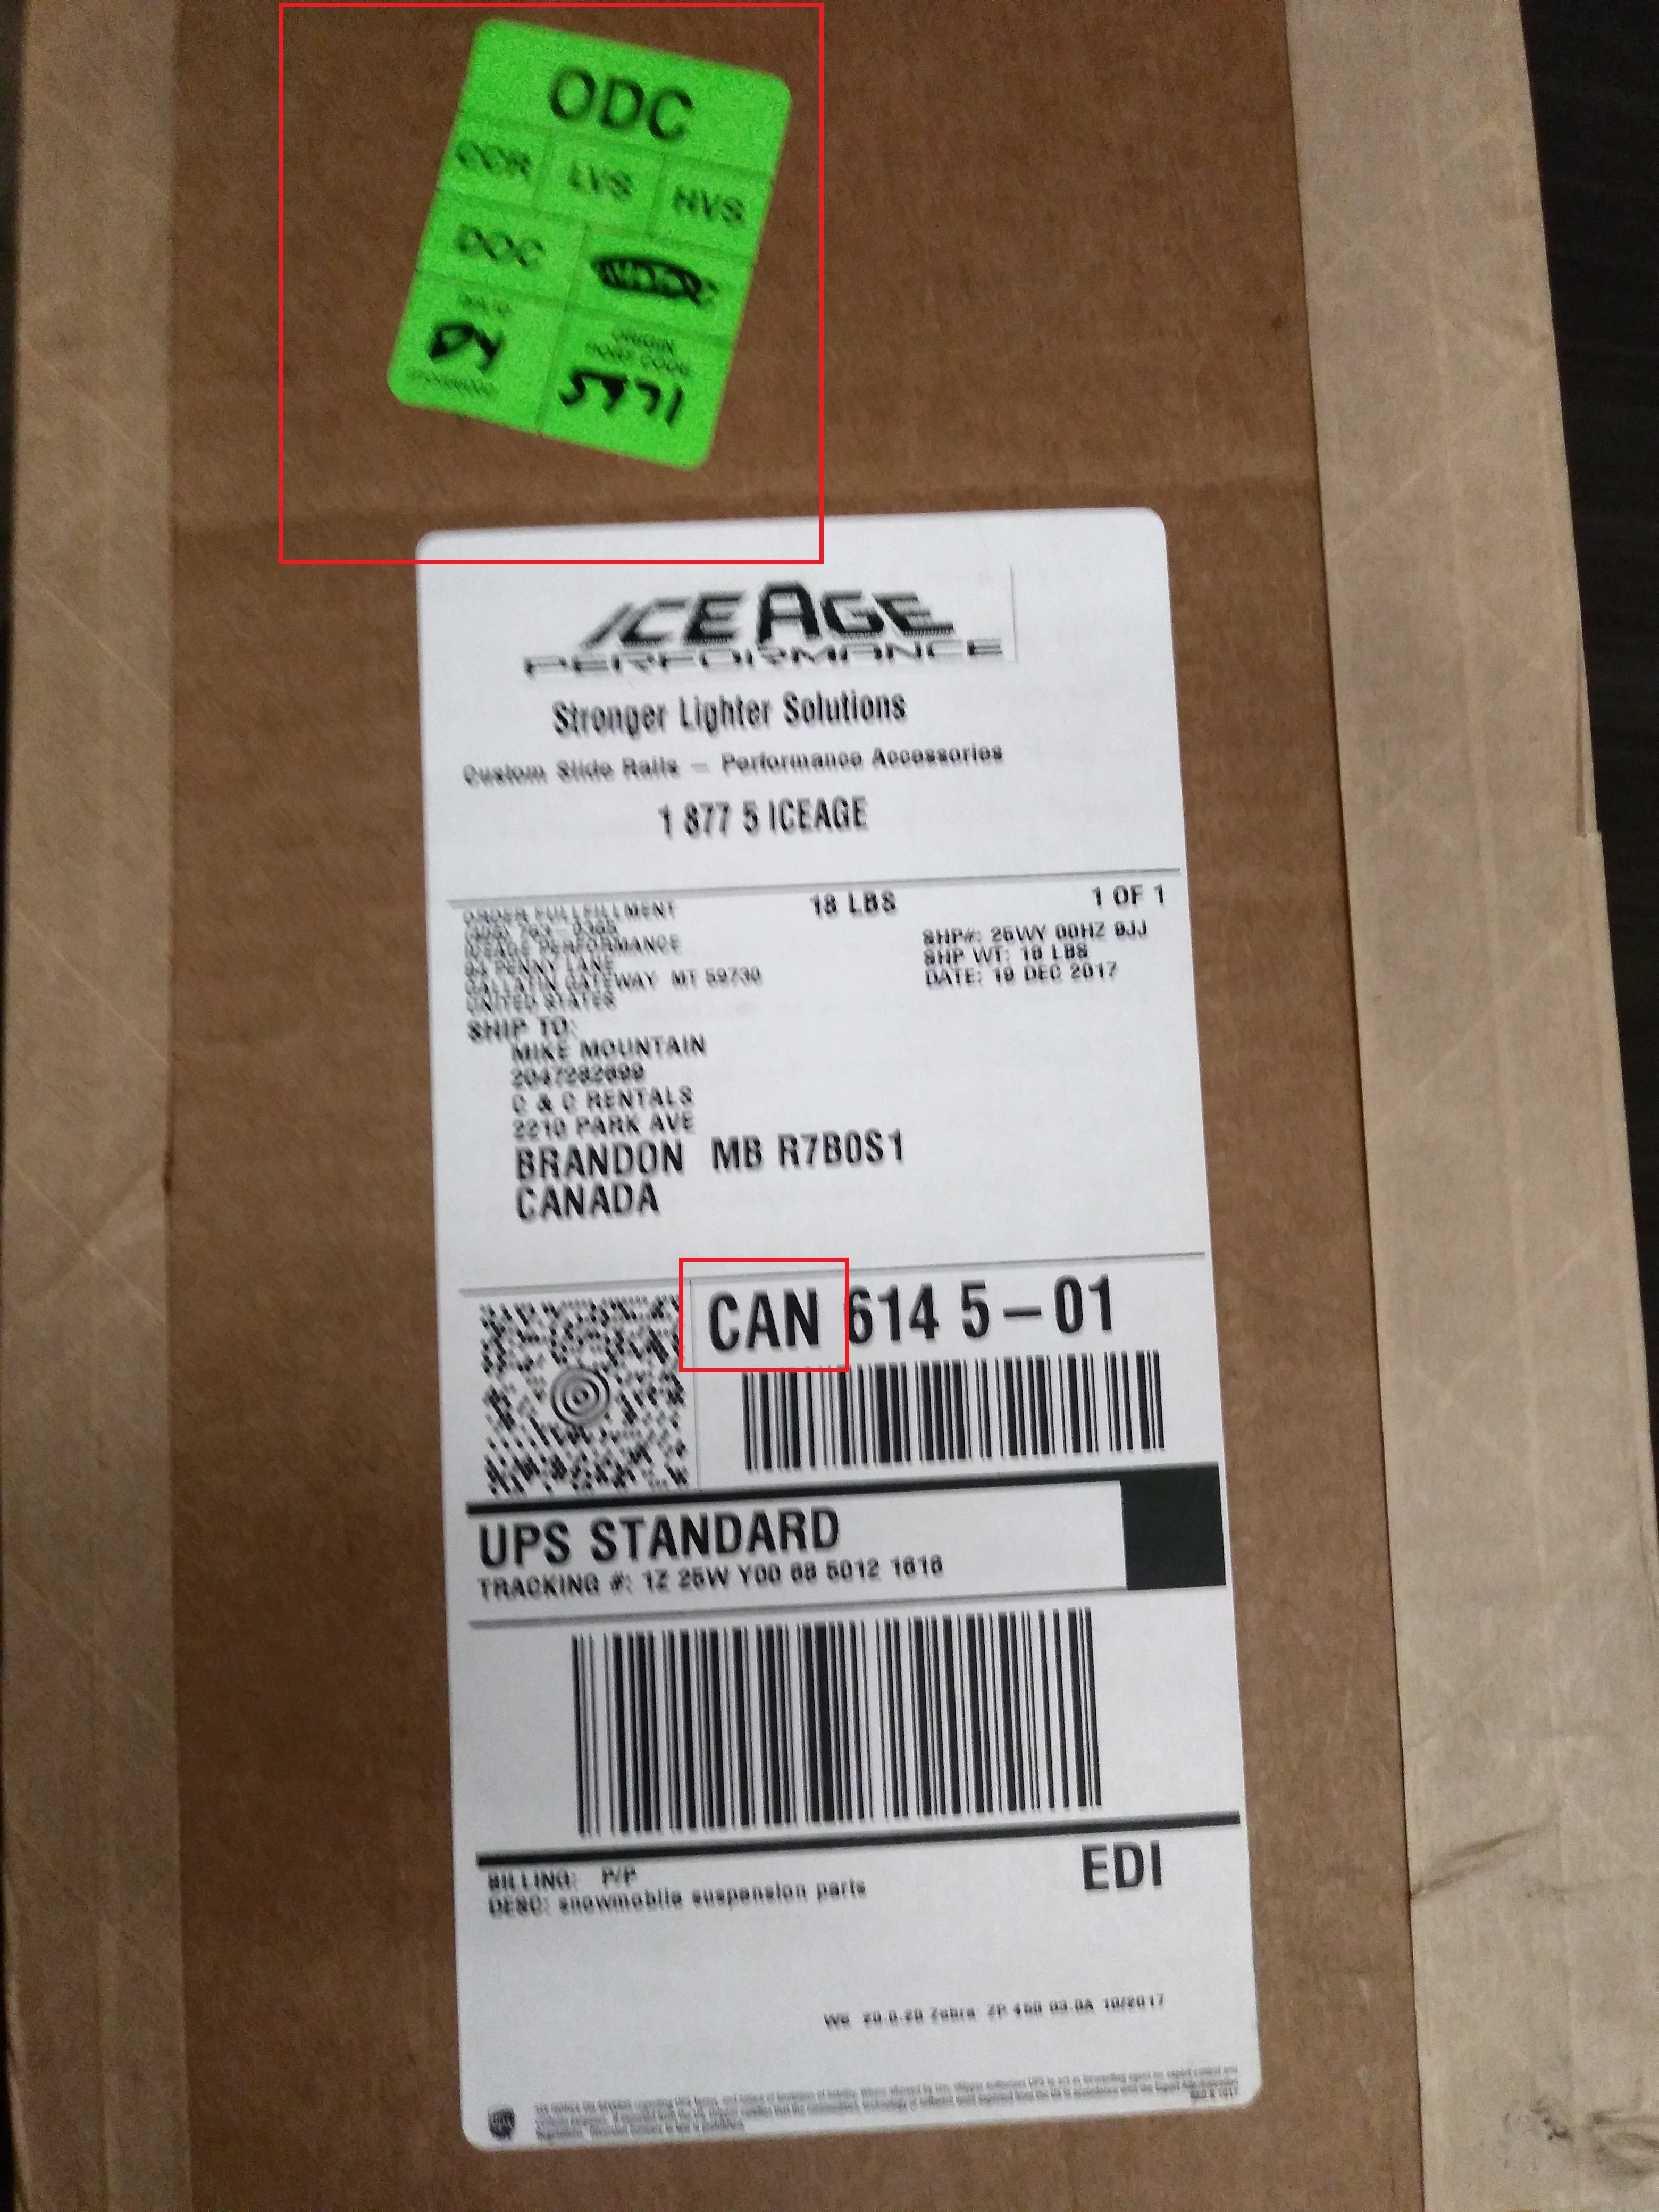
\includegraphics[angle=90,width=0.4\linewidth]{20171221_163826}
    \caption{MB Canada with green sticker}
\end{figure}

\subsubsection{Next Days}
A significant portion of UPS volume carries a service level of "Next Day". Given the cost and priority associated with these packages they are often handled via UPS Air. 

\begin{itemize}
    \item All MN next day packages can be sorted accordingly.
    \item Most of the border state (ND, SD, IA, WI) volume can also be sorted, but you should check with your supervisor for exceptions.
    \item All other out-state next day volume needs to go to the next day bin to be brought to the air pull by the end of the night.
\end{itemize}

\begin{figure}[H]
\begin{subfigure}{0.5\textwidth}
\centering
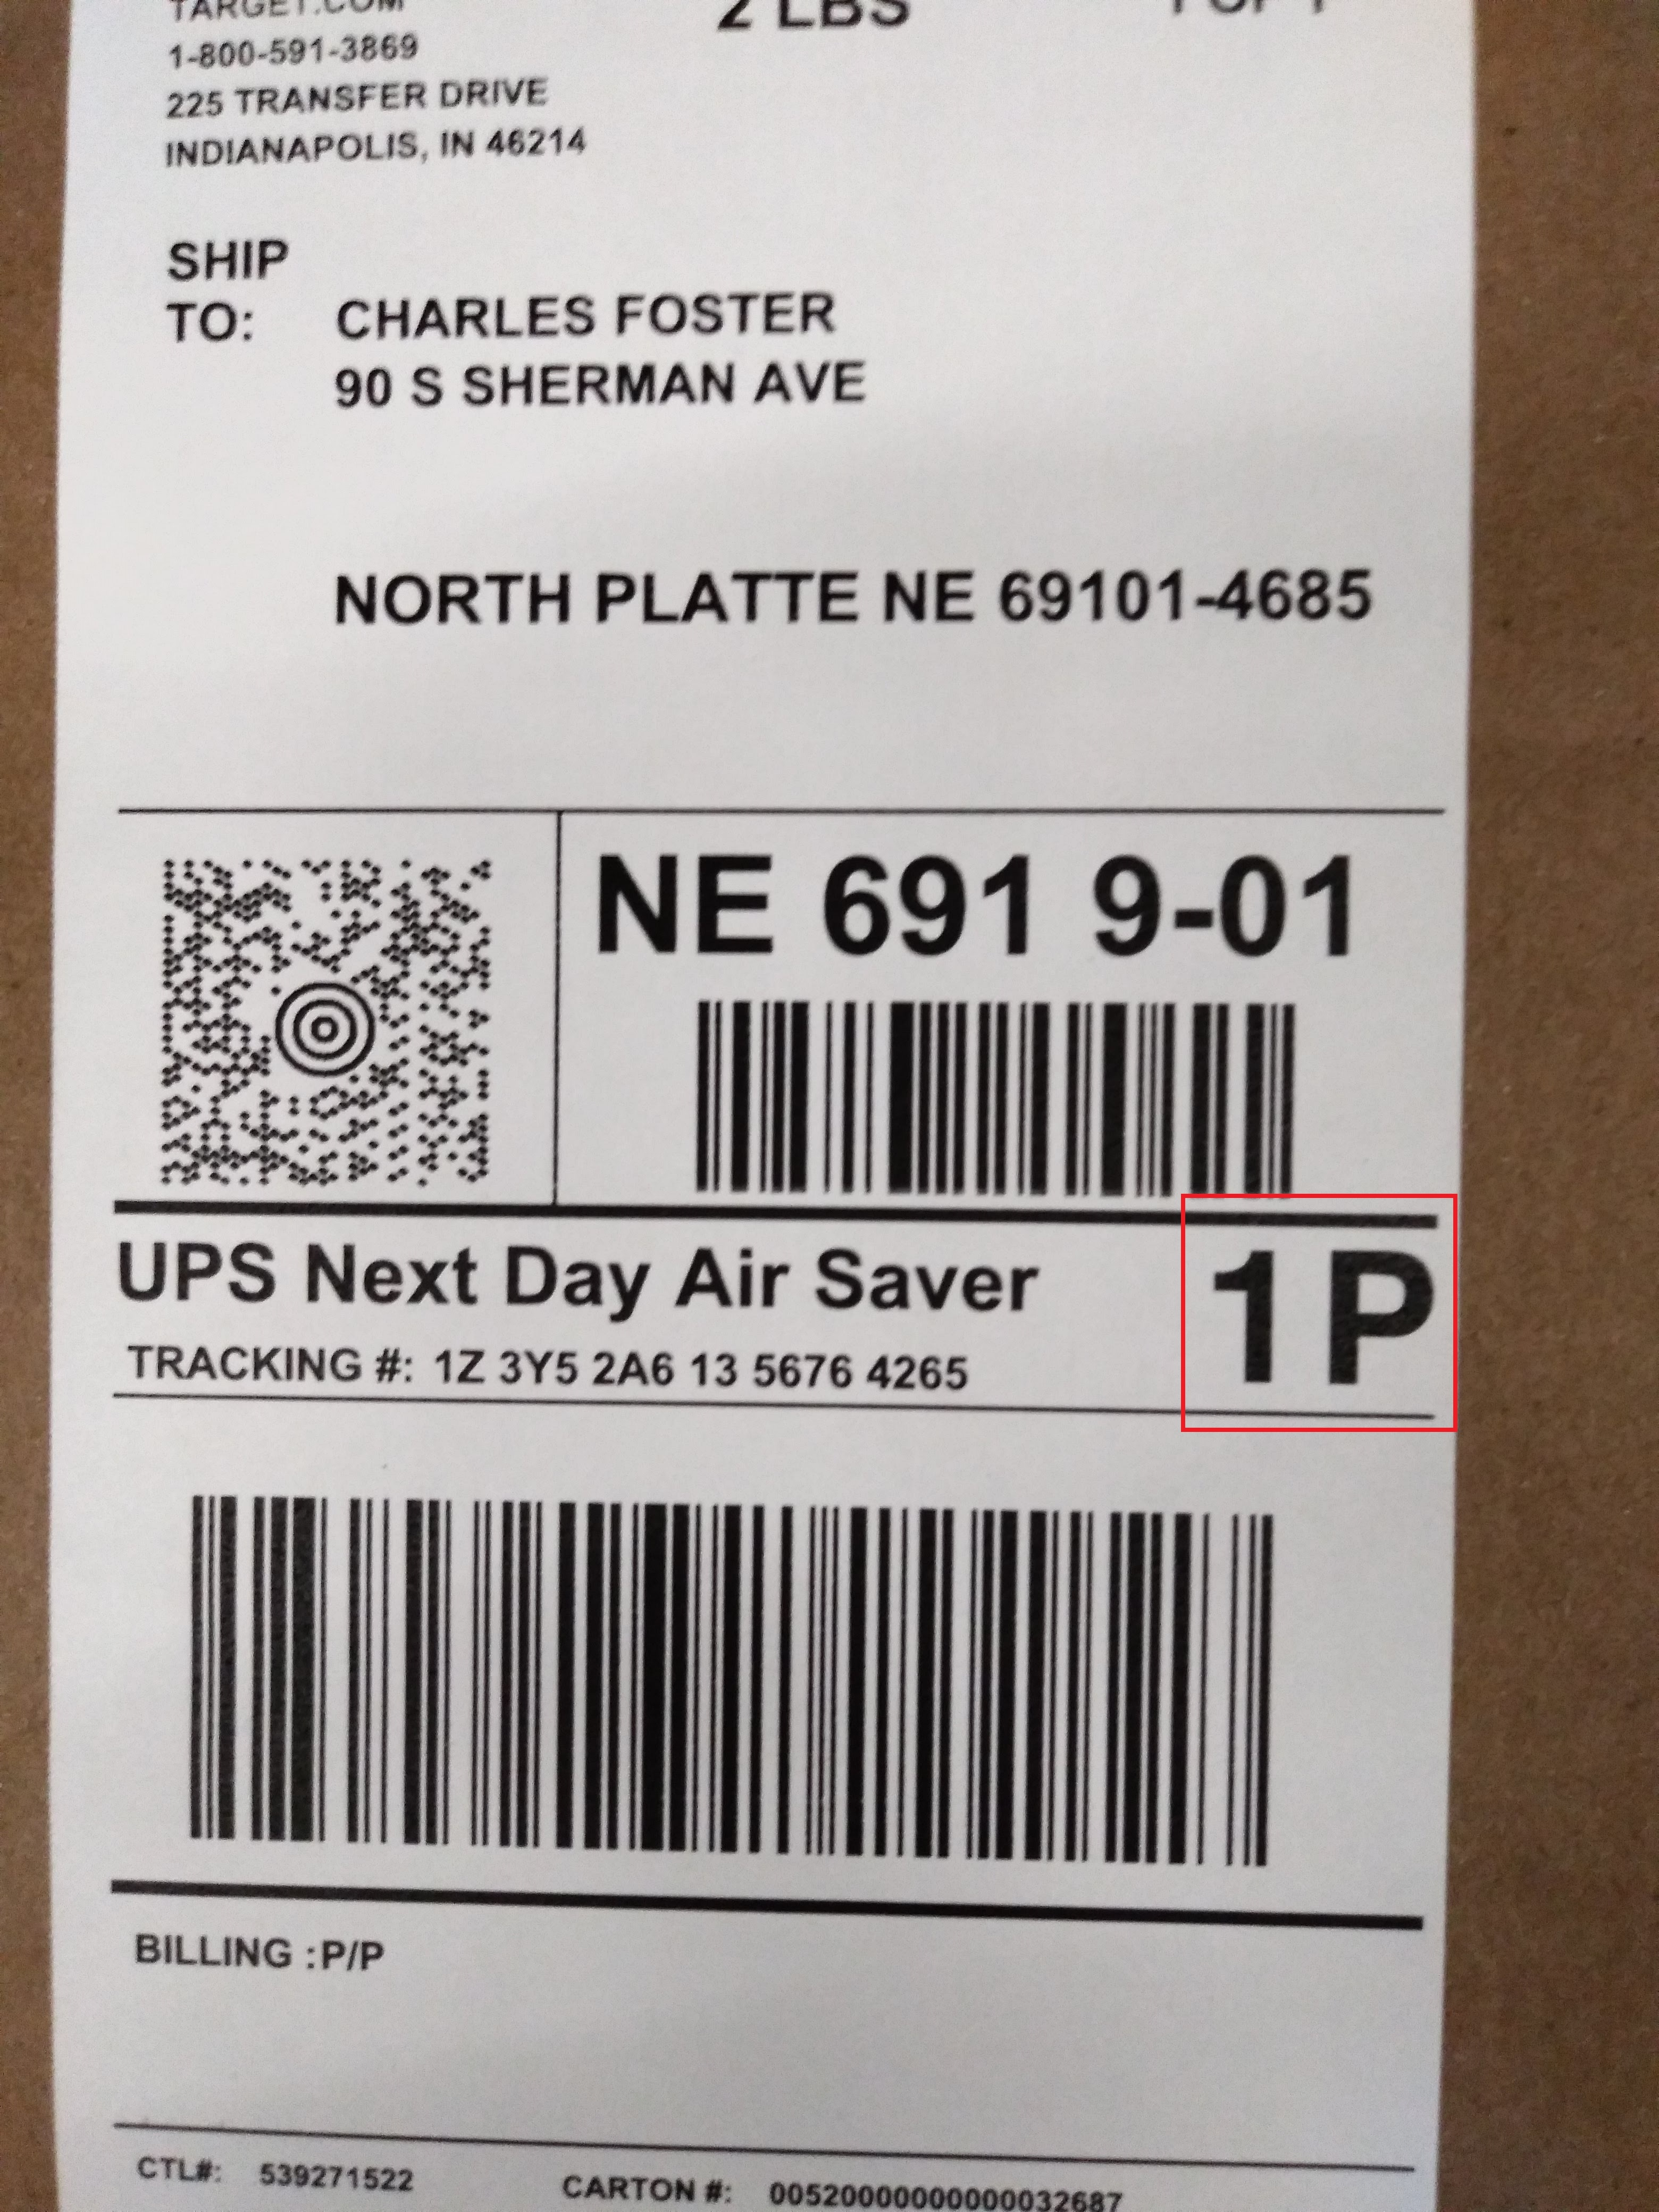
\includegraphics[angle=90,width=0.7\linewidth]{20171221_160249} 
\caption{Next Day Package}
\end{subfigure}
\begin{subfigure}{0.5\textwidth}
\centering
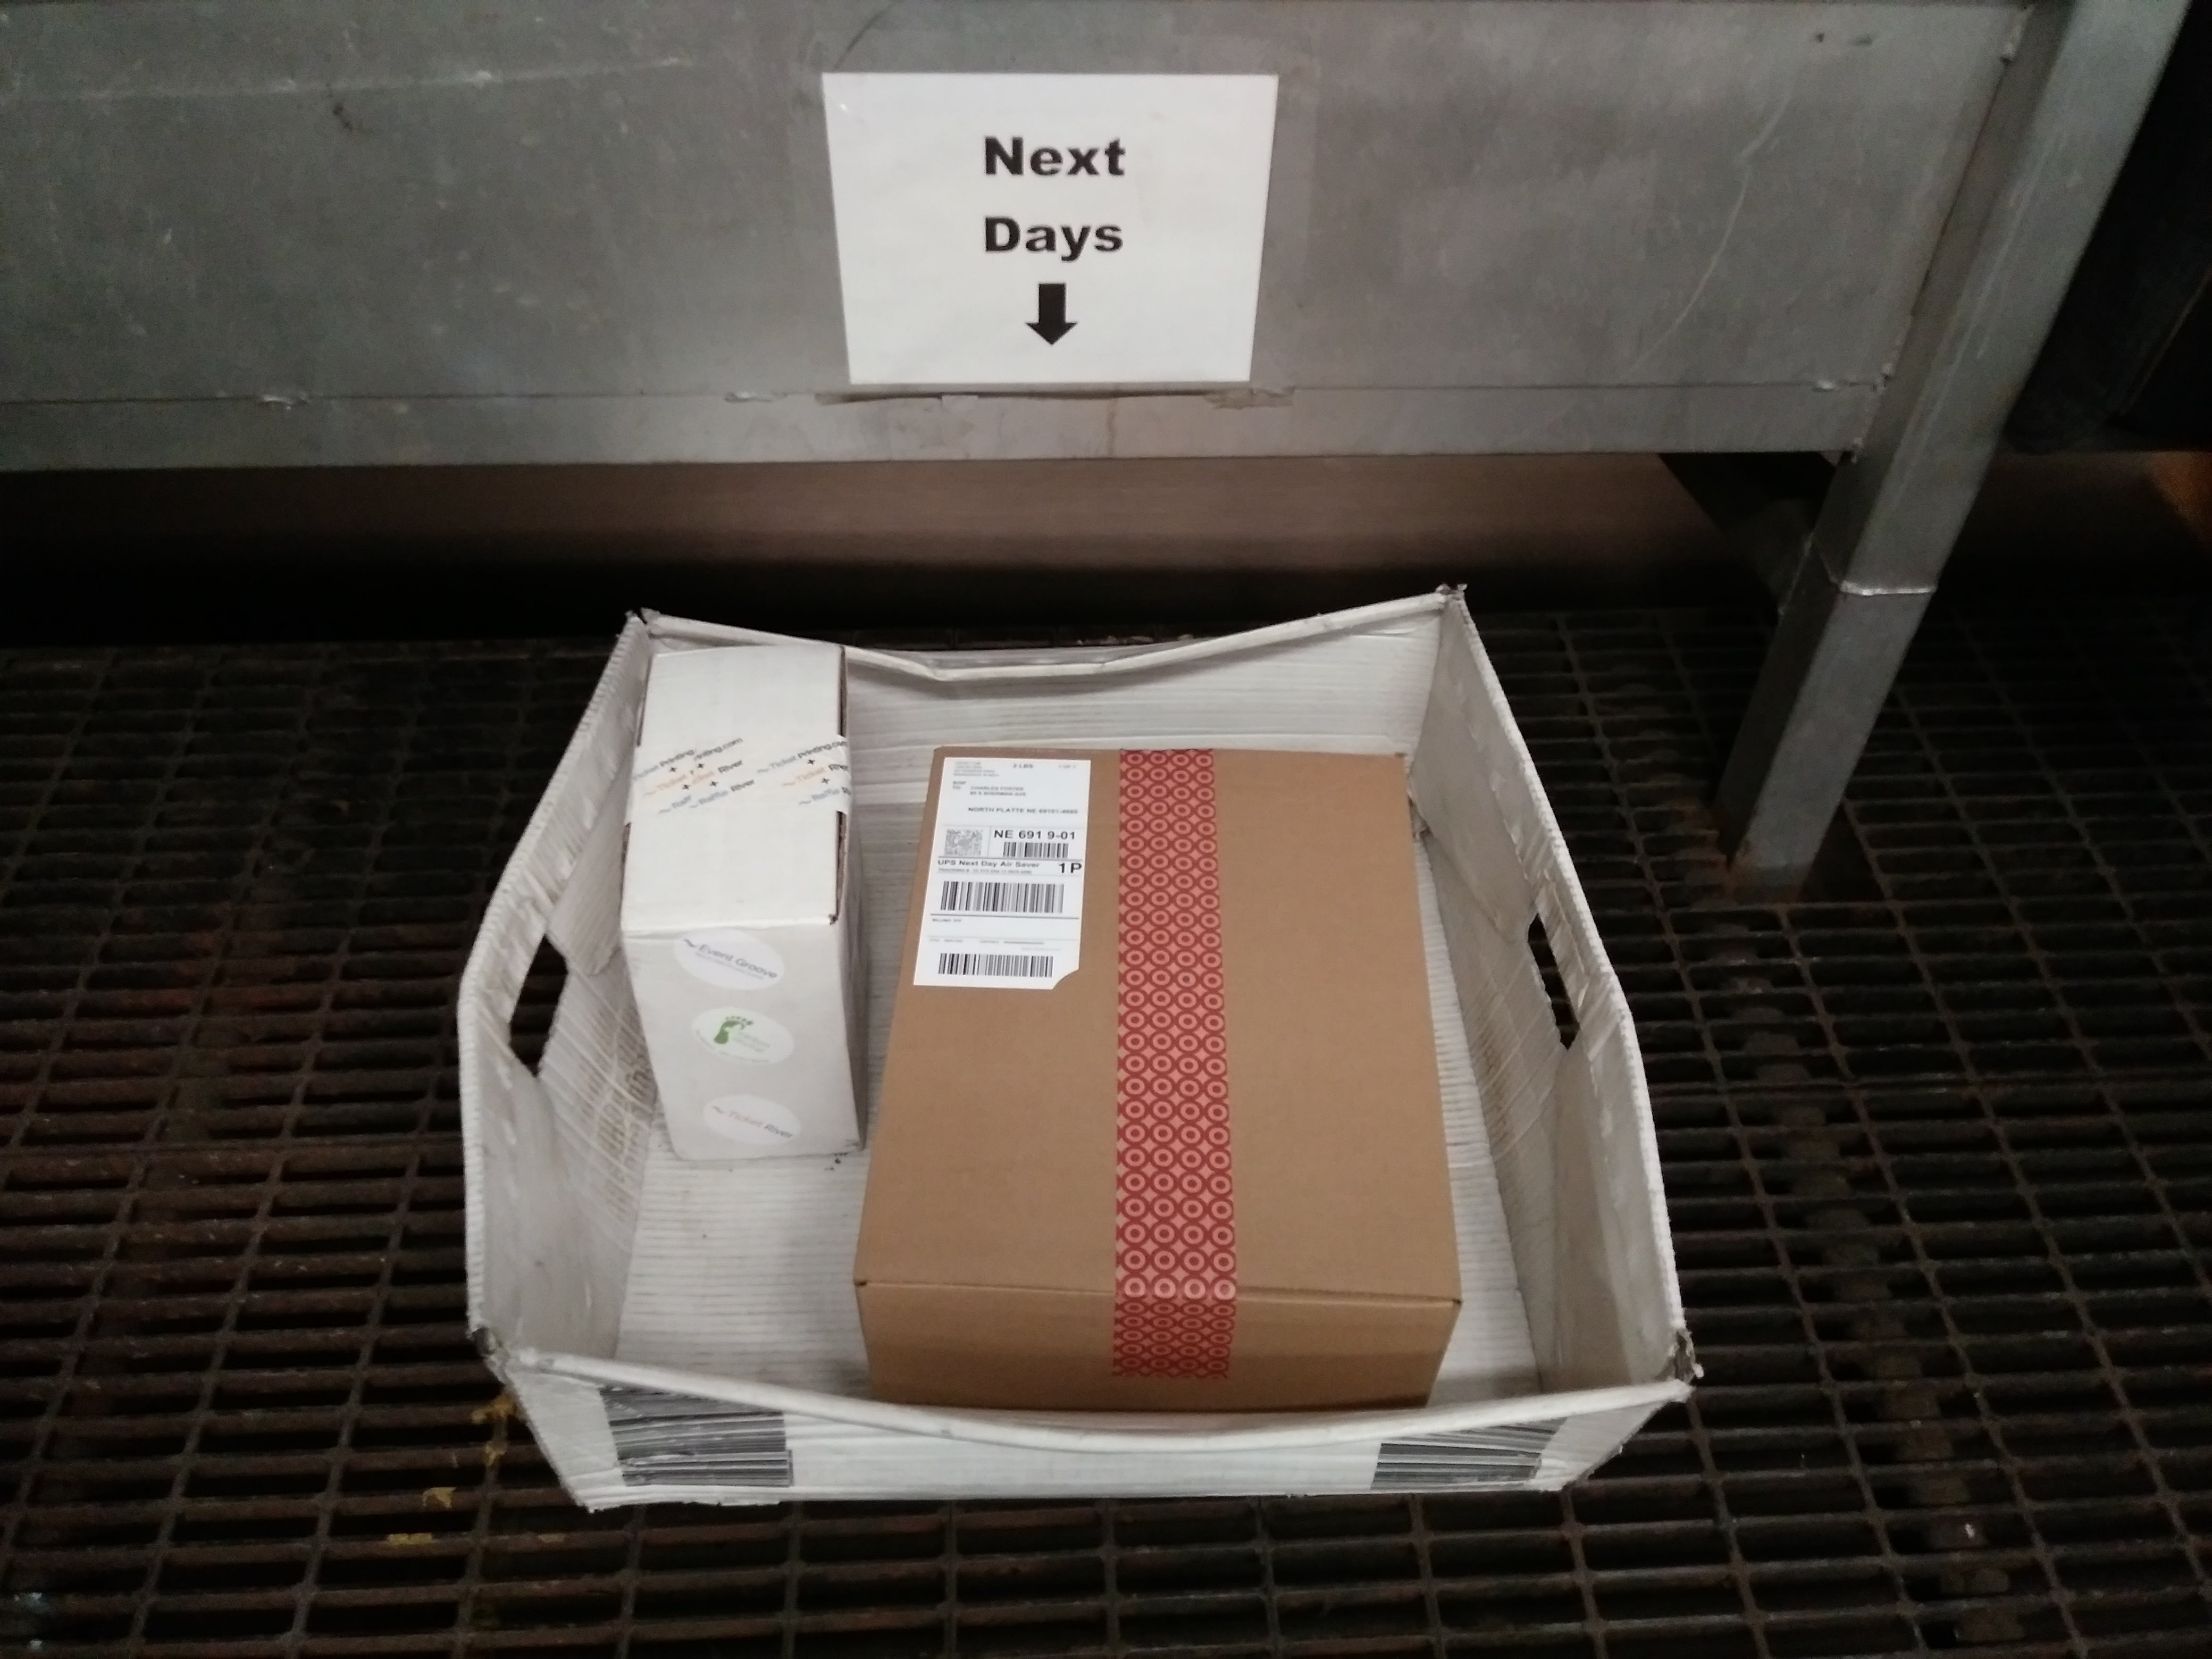
\includegraphics[width=0.7\linewidth]{20171221_161216}
\caption{Next Day Bin}
\end{subfigure}
\end{figure}

\subsubsection{Expedited International}
Given UPS' status as one of the largest courier services in the world, we often deal with international volume that extends beyond North America. While there is a destination to sort general international packages to, some of this volume may be expedited and should be handled differently.
\begin{itemize}
    \item Expedited international = any 2day or less non-Canada/US/Mexico package.
    \item These need to be set aside and put in the "Next Day" bin to be brought to the Air Pull by the end of the night.
\end{itemize}

\begin{figure}[H]
    \centering
    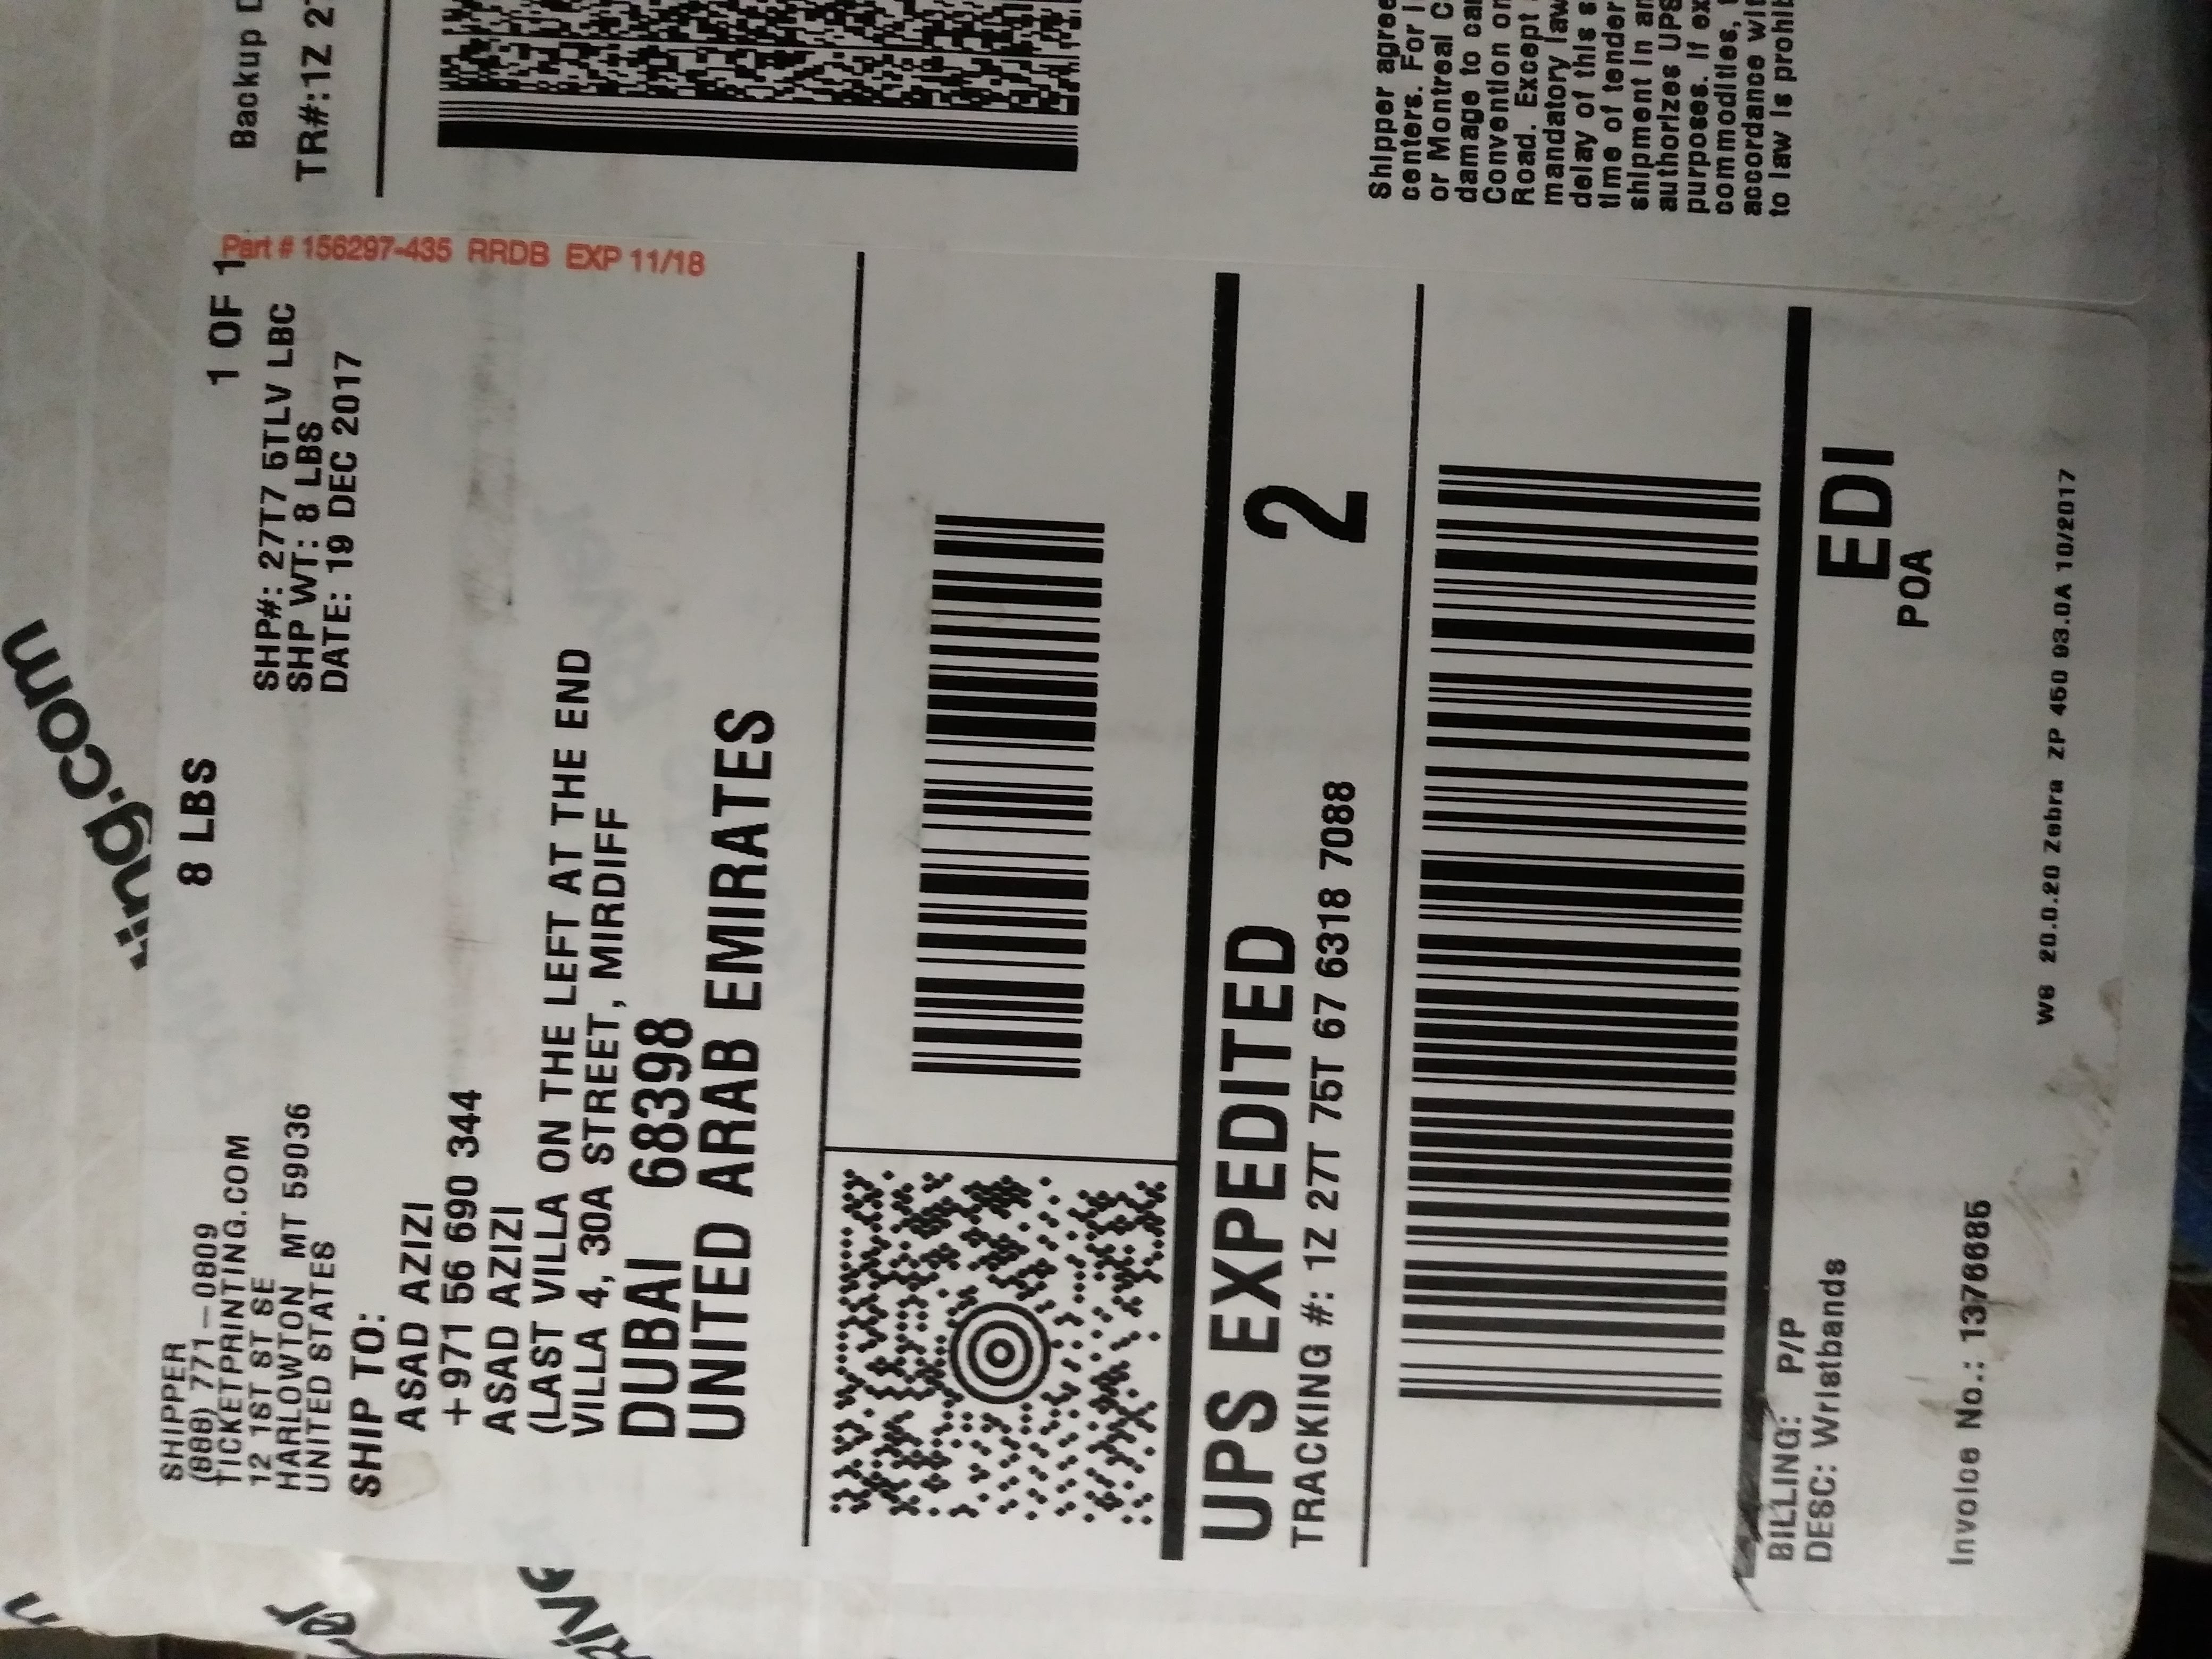
\includegraphics[width=0.4\linewidth]{20171221_161139}
    \caption{}
\end{figure}

\subsubsection{Return Service/Multiple Labels}
It is a common occurrence to come across a package on a multi-leg trip. A few instances where this might come about are the recipient refusing delivery, the recipient delivering the same package to the actual destination, or a general return to a retailer. In all of these cases, there is a good chance that multiple labels will be on the box which can result in the package ending up at the wrong destination. 

\begin{itemize}
    \item Evaluate the box if you find more than one unmarked label. Look for notation or an order of operation in delivery destinations that would indicate the true destination.
    \item After determining the correct destination, use a black pen to write a vertical line through all incorrect bar codes, rendering it unscannable. 
\end{itemize}

\begin{figure}[H]
    \centering
    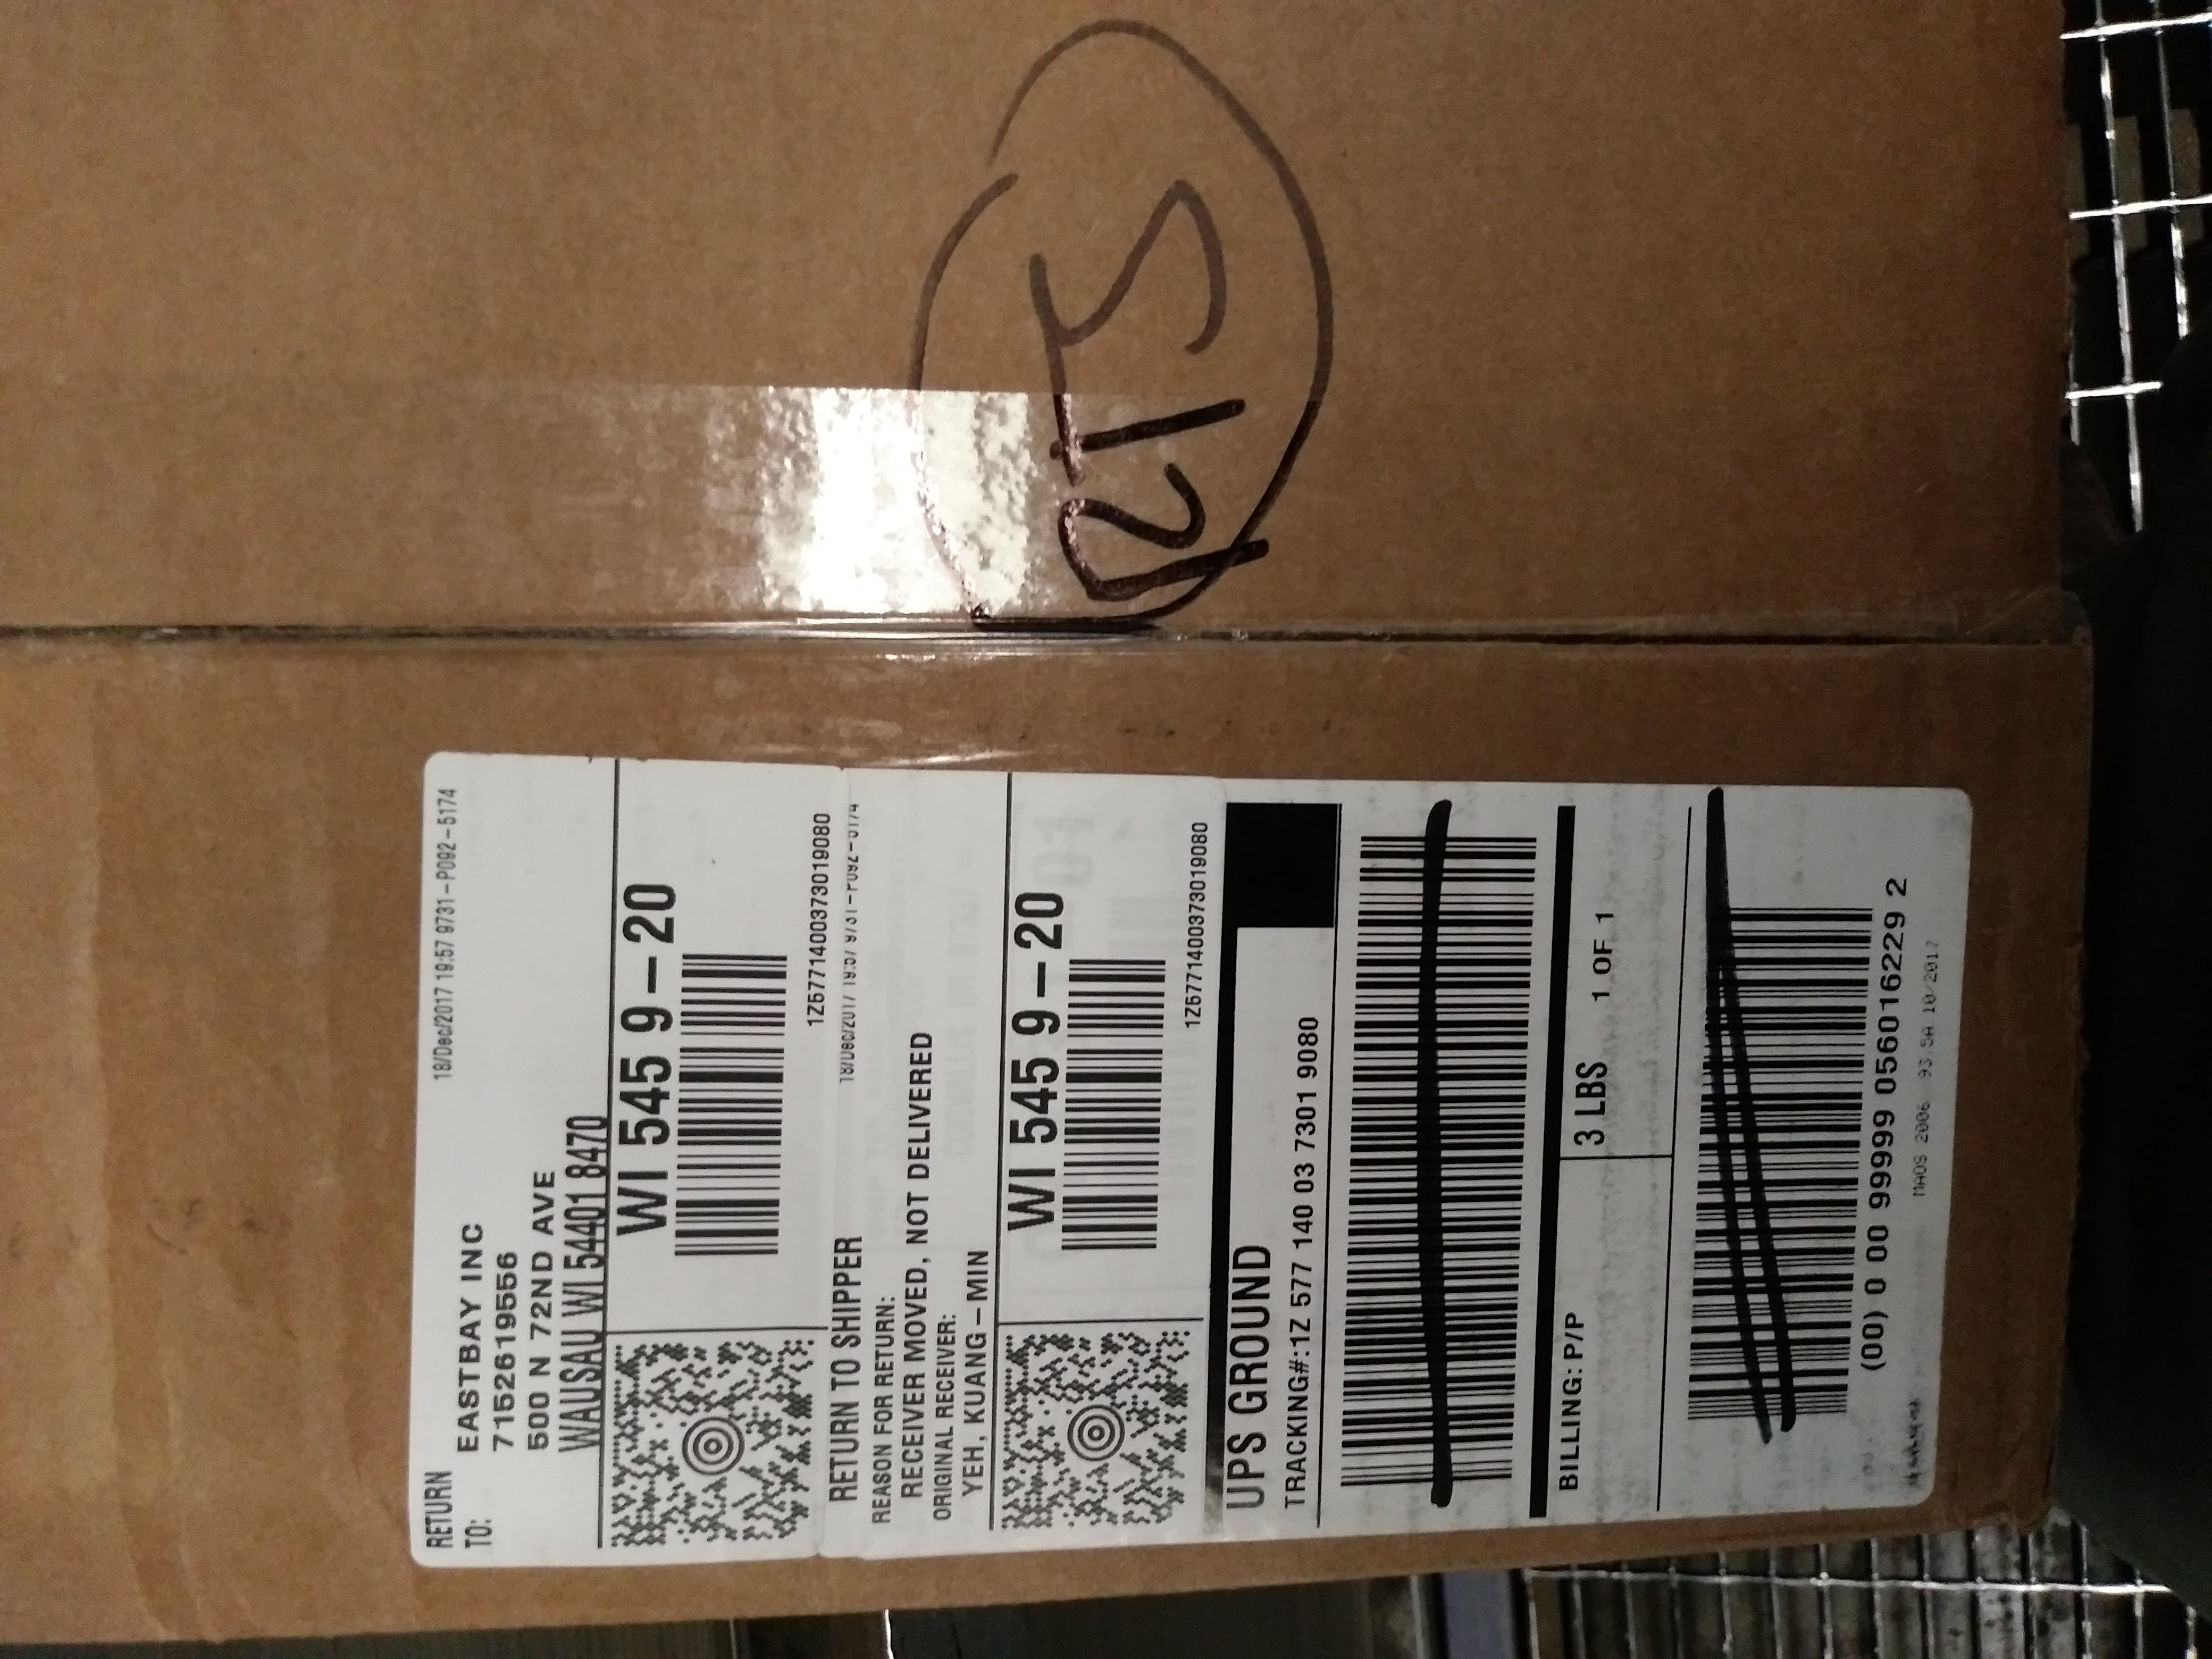
\includegraphics[width=0.4\linewidth]{20171221_171958}
    \caption{Returned Package}
\end{figure}

\clearpage

\subsection{Common Missorts}

\begin{figure}[H]
\begin{subfigure}{0.5\textwidth}
\centering
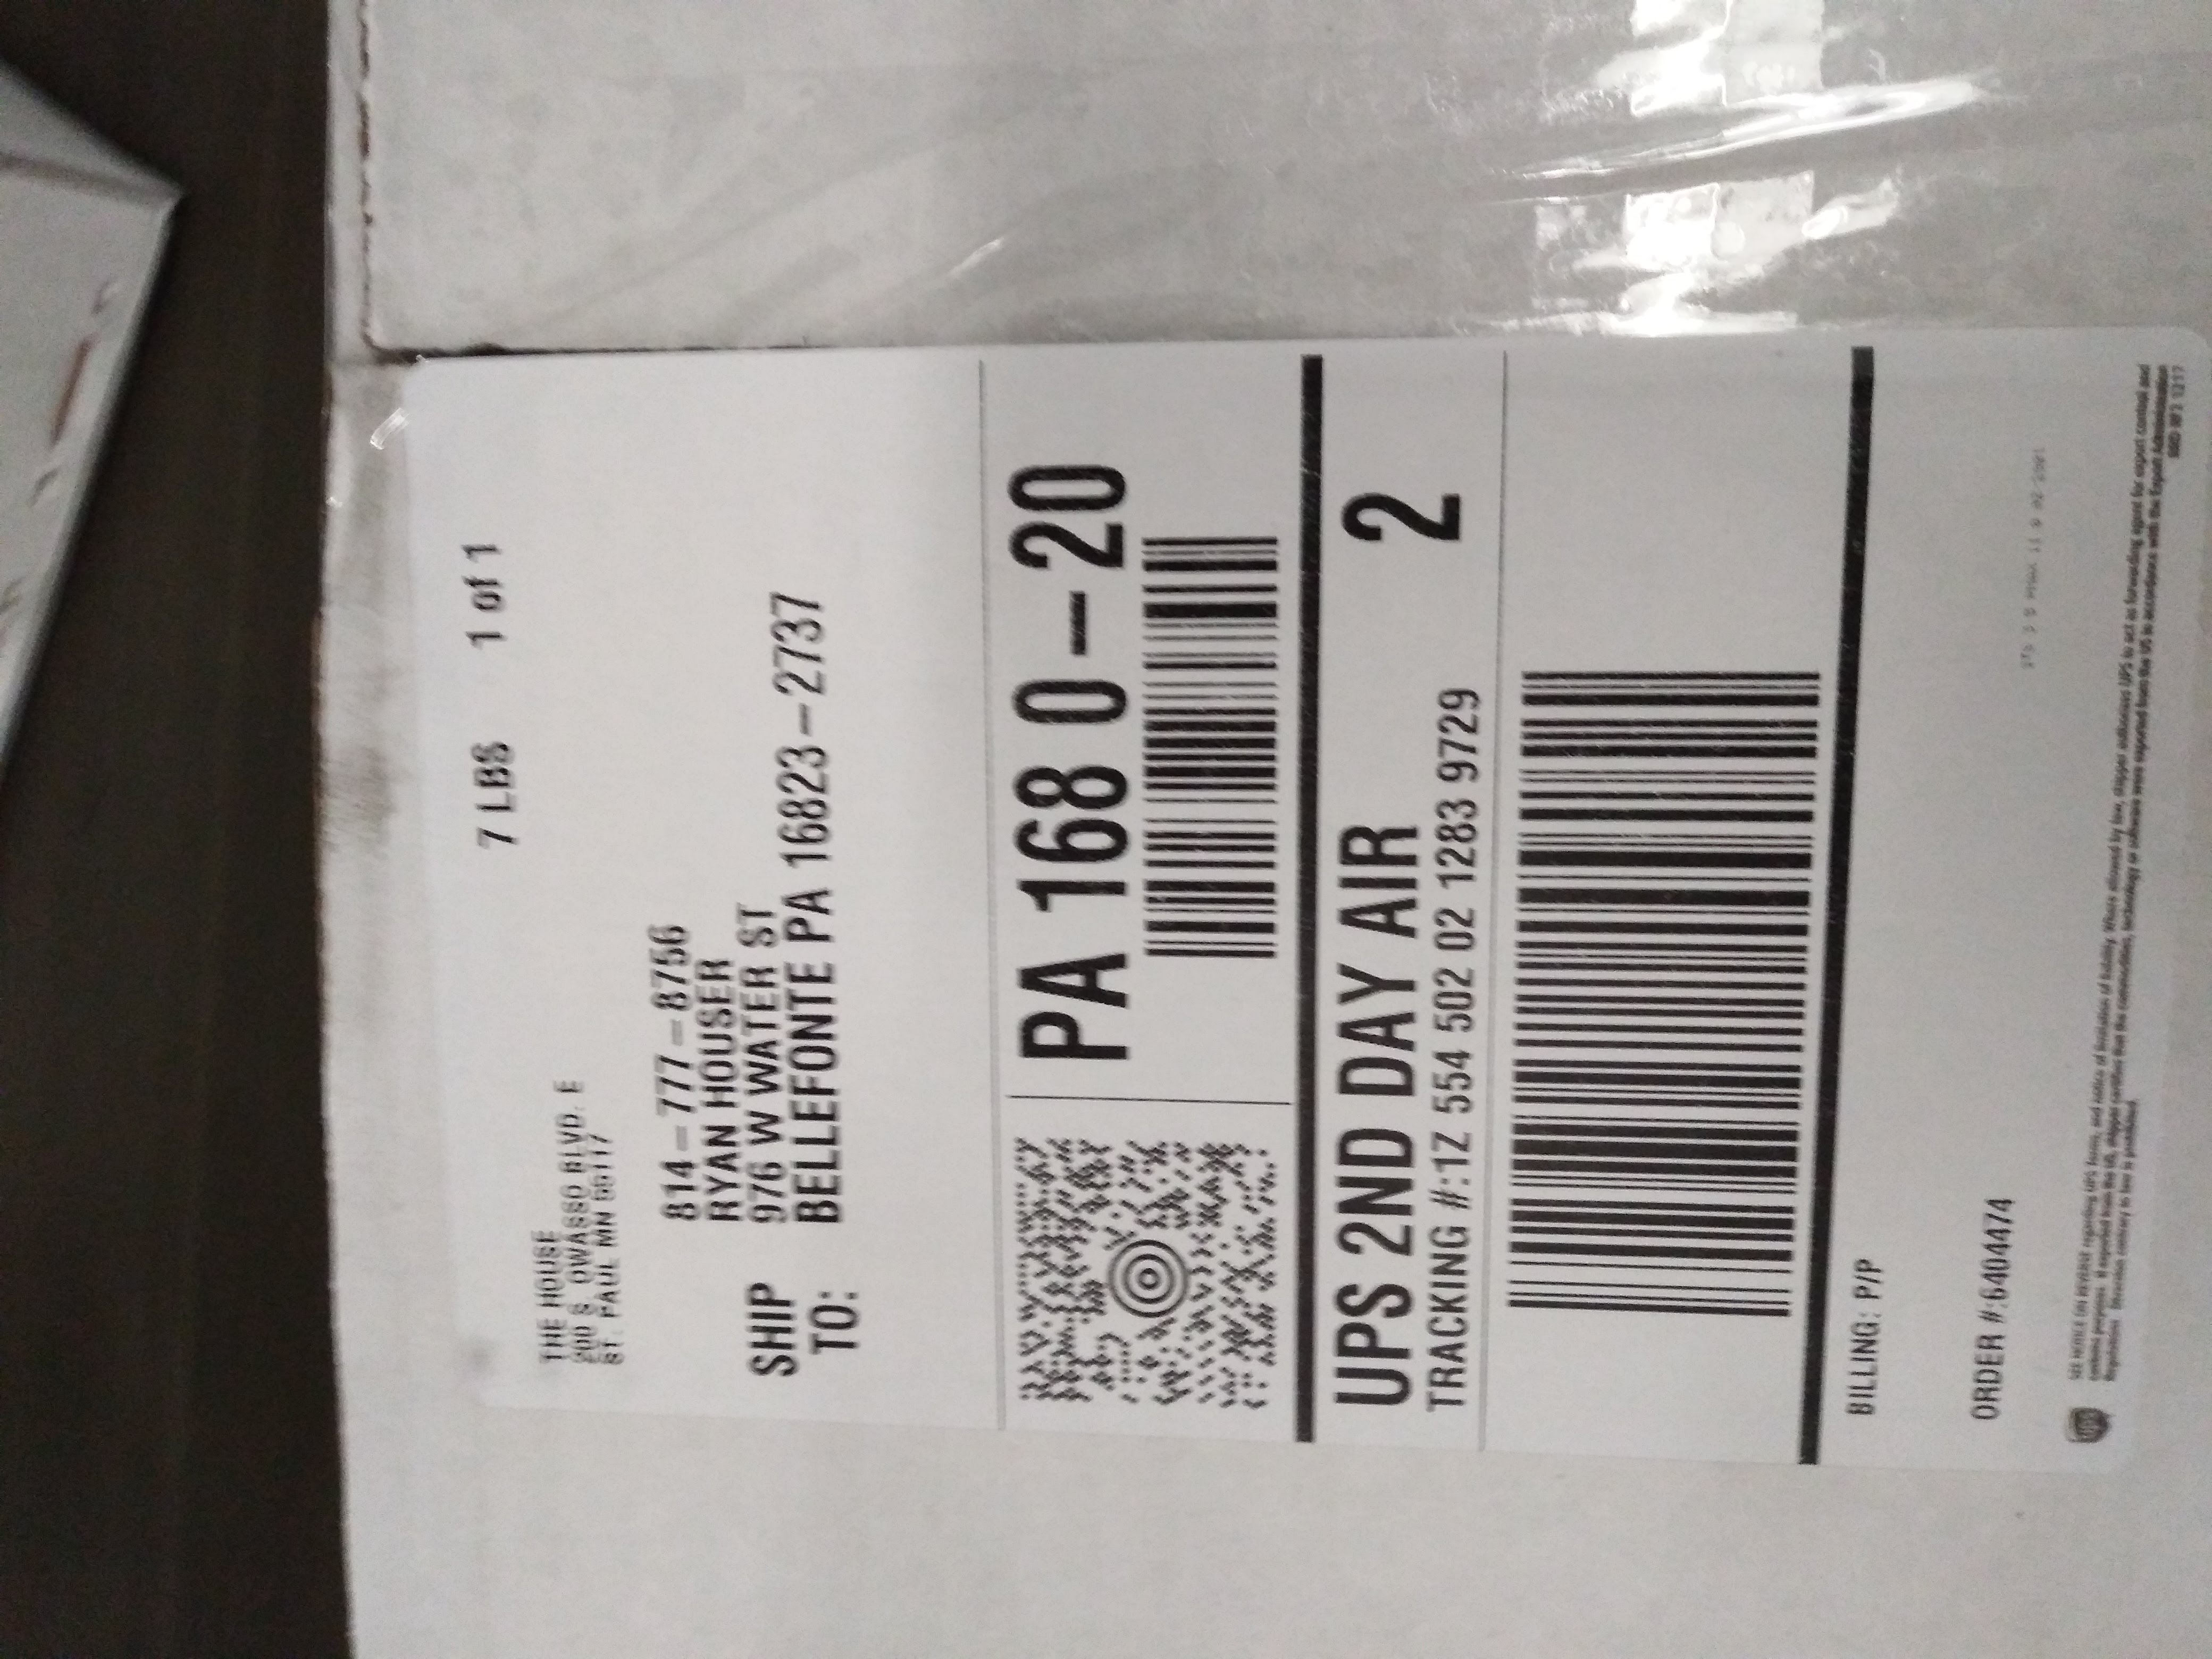
\includegraphics[width=0.7\linewidth]{20180102_174408} 
\caption{PA Service Level Exception}
\end{subfigure}
\begin{subfigure}{0.5\textwidth}
\centering
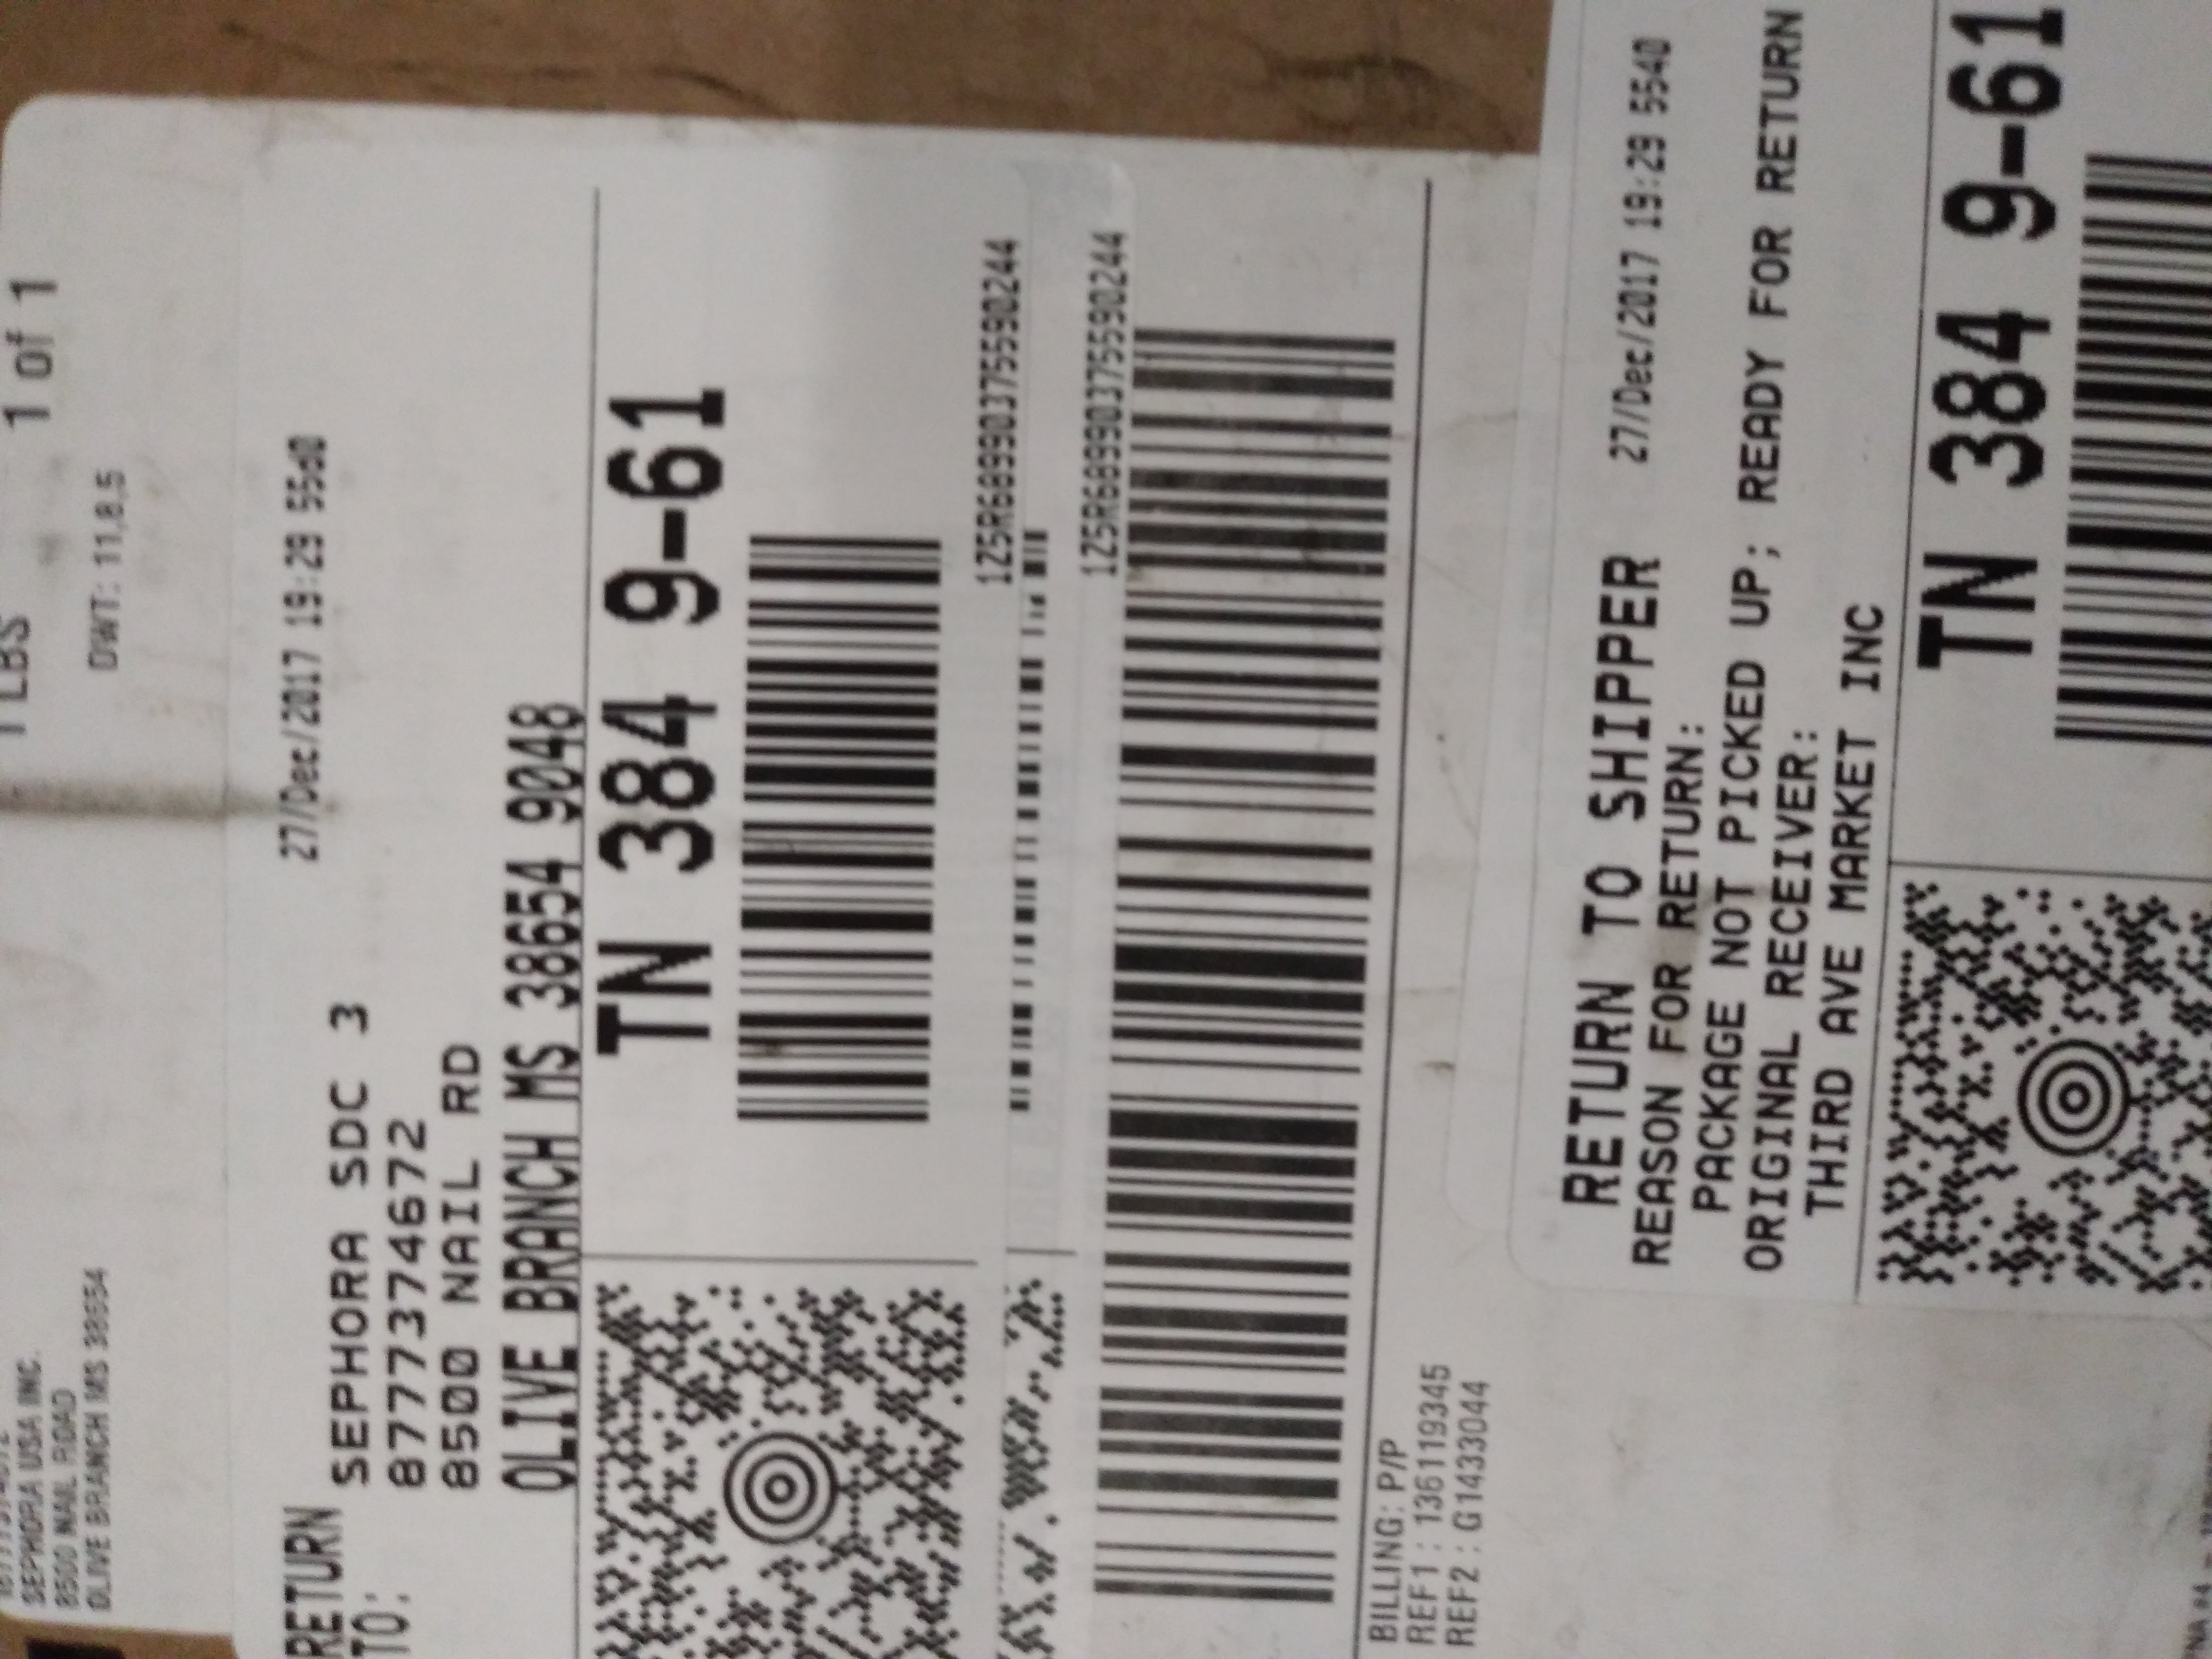
\includegraphics[width=0.7\linewidth]{20171227_200358} 
\caption{MS - TN Discrepancy}
\end{subfigure}
\begin{subfigure}{0.5\textwidth}
\centering
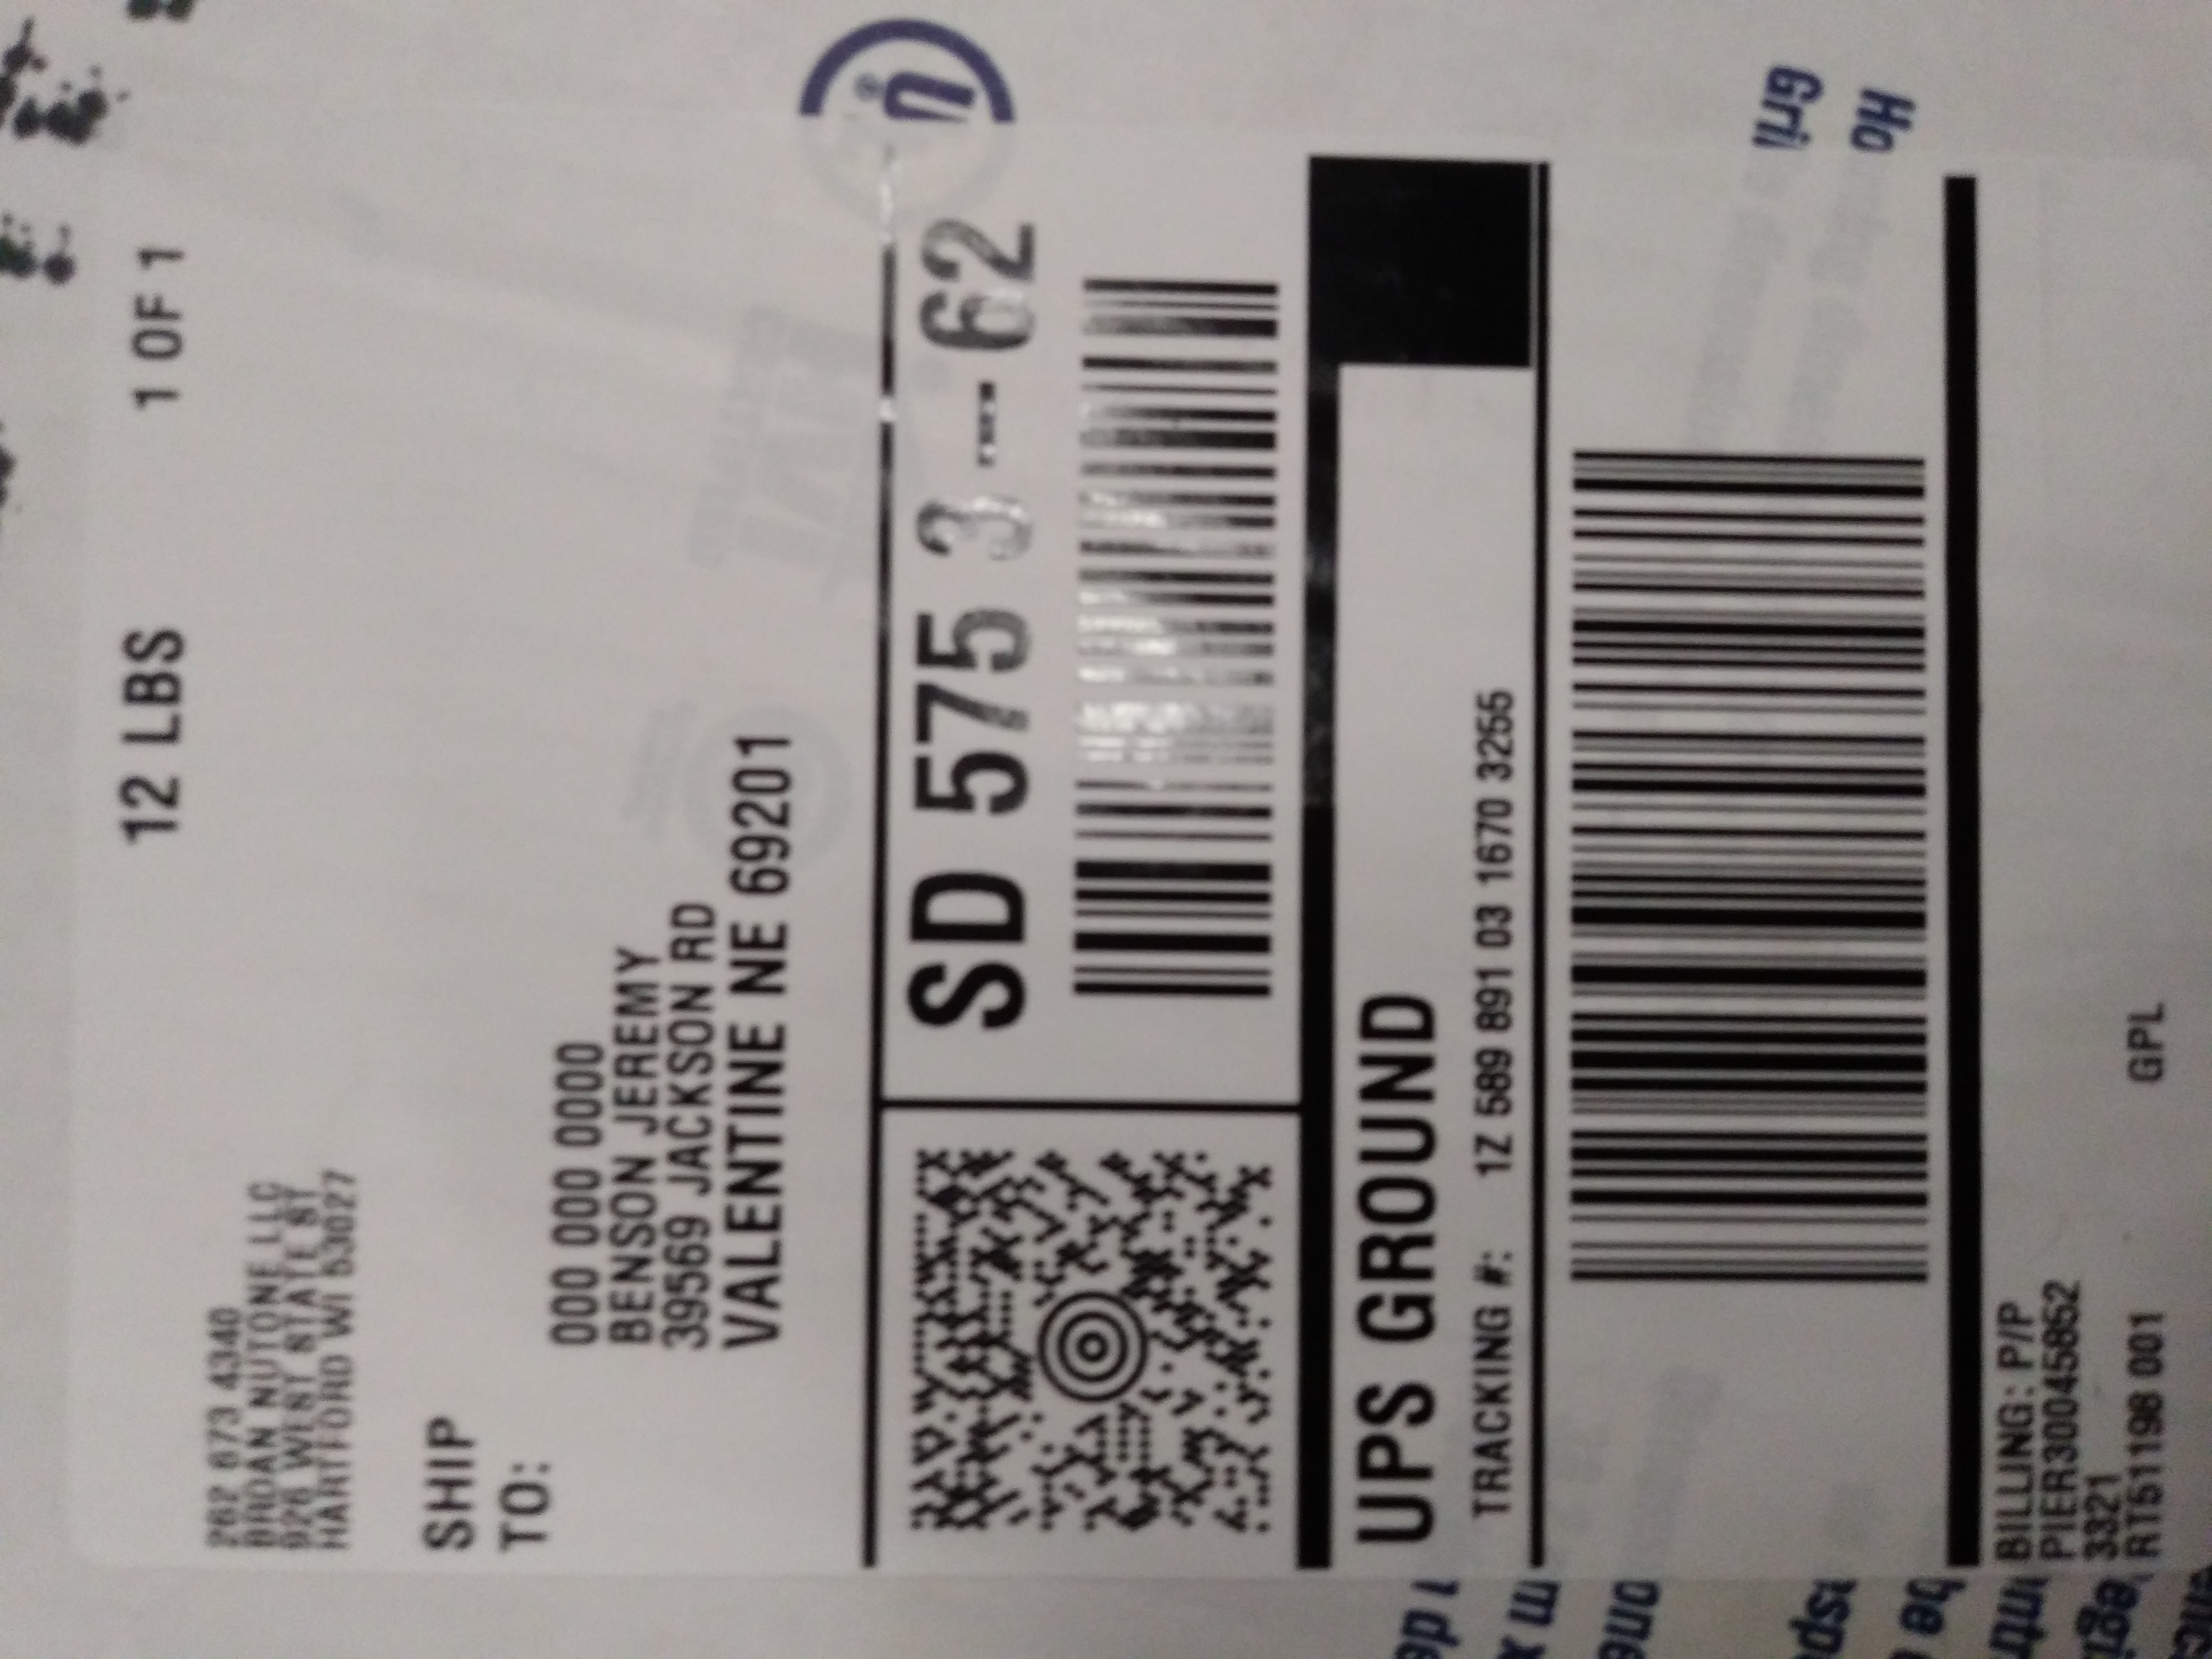
\includegraphics[width=0.7\linewidth]{20171222_194105} 
\caption{NE Exception}
\end{subfigure}
\begin{subfigure}{0.5\textwidth}
\centering
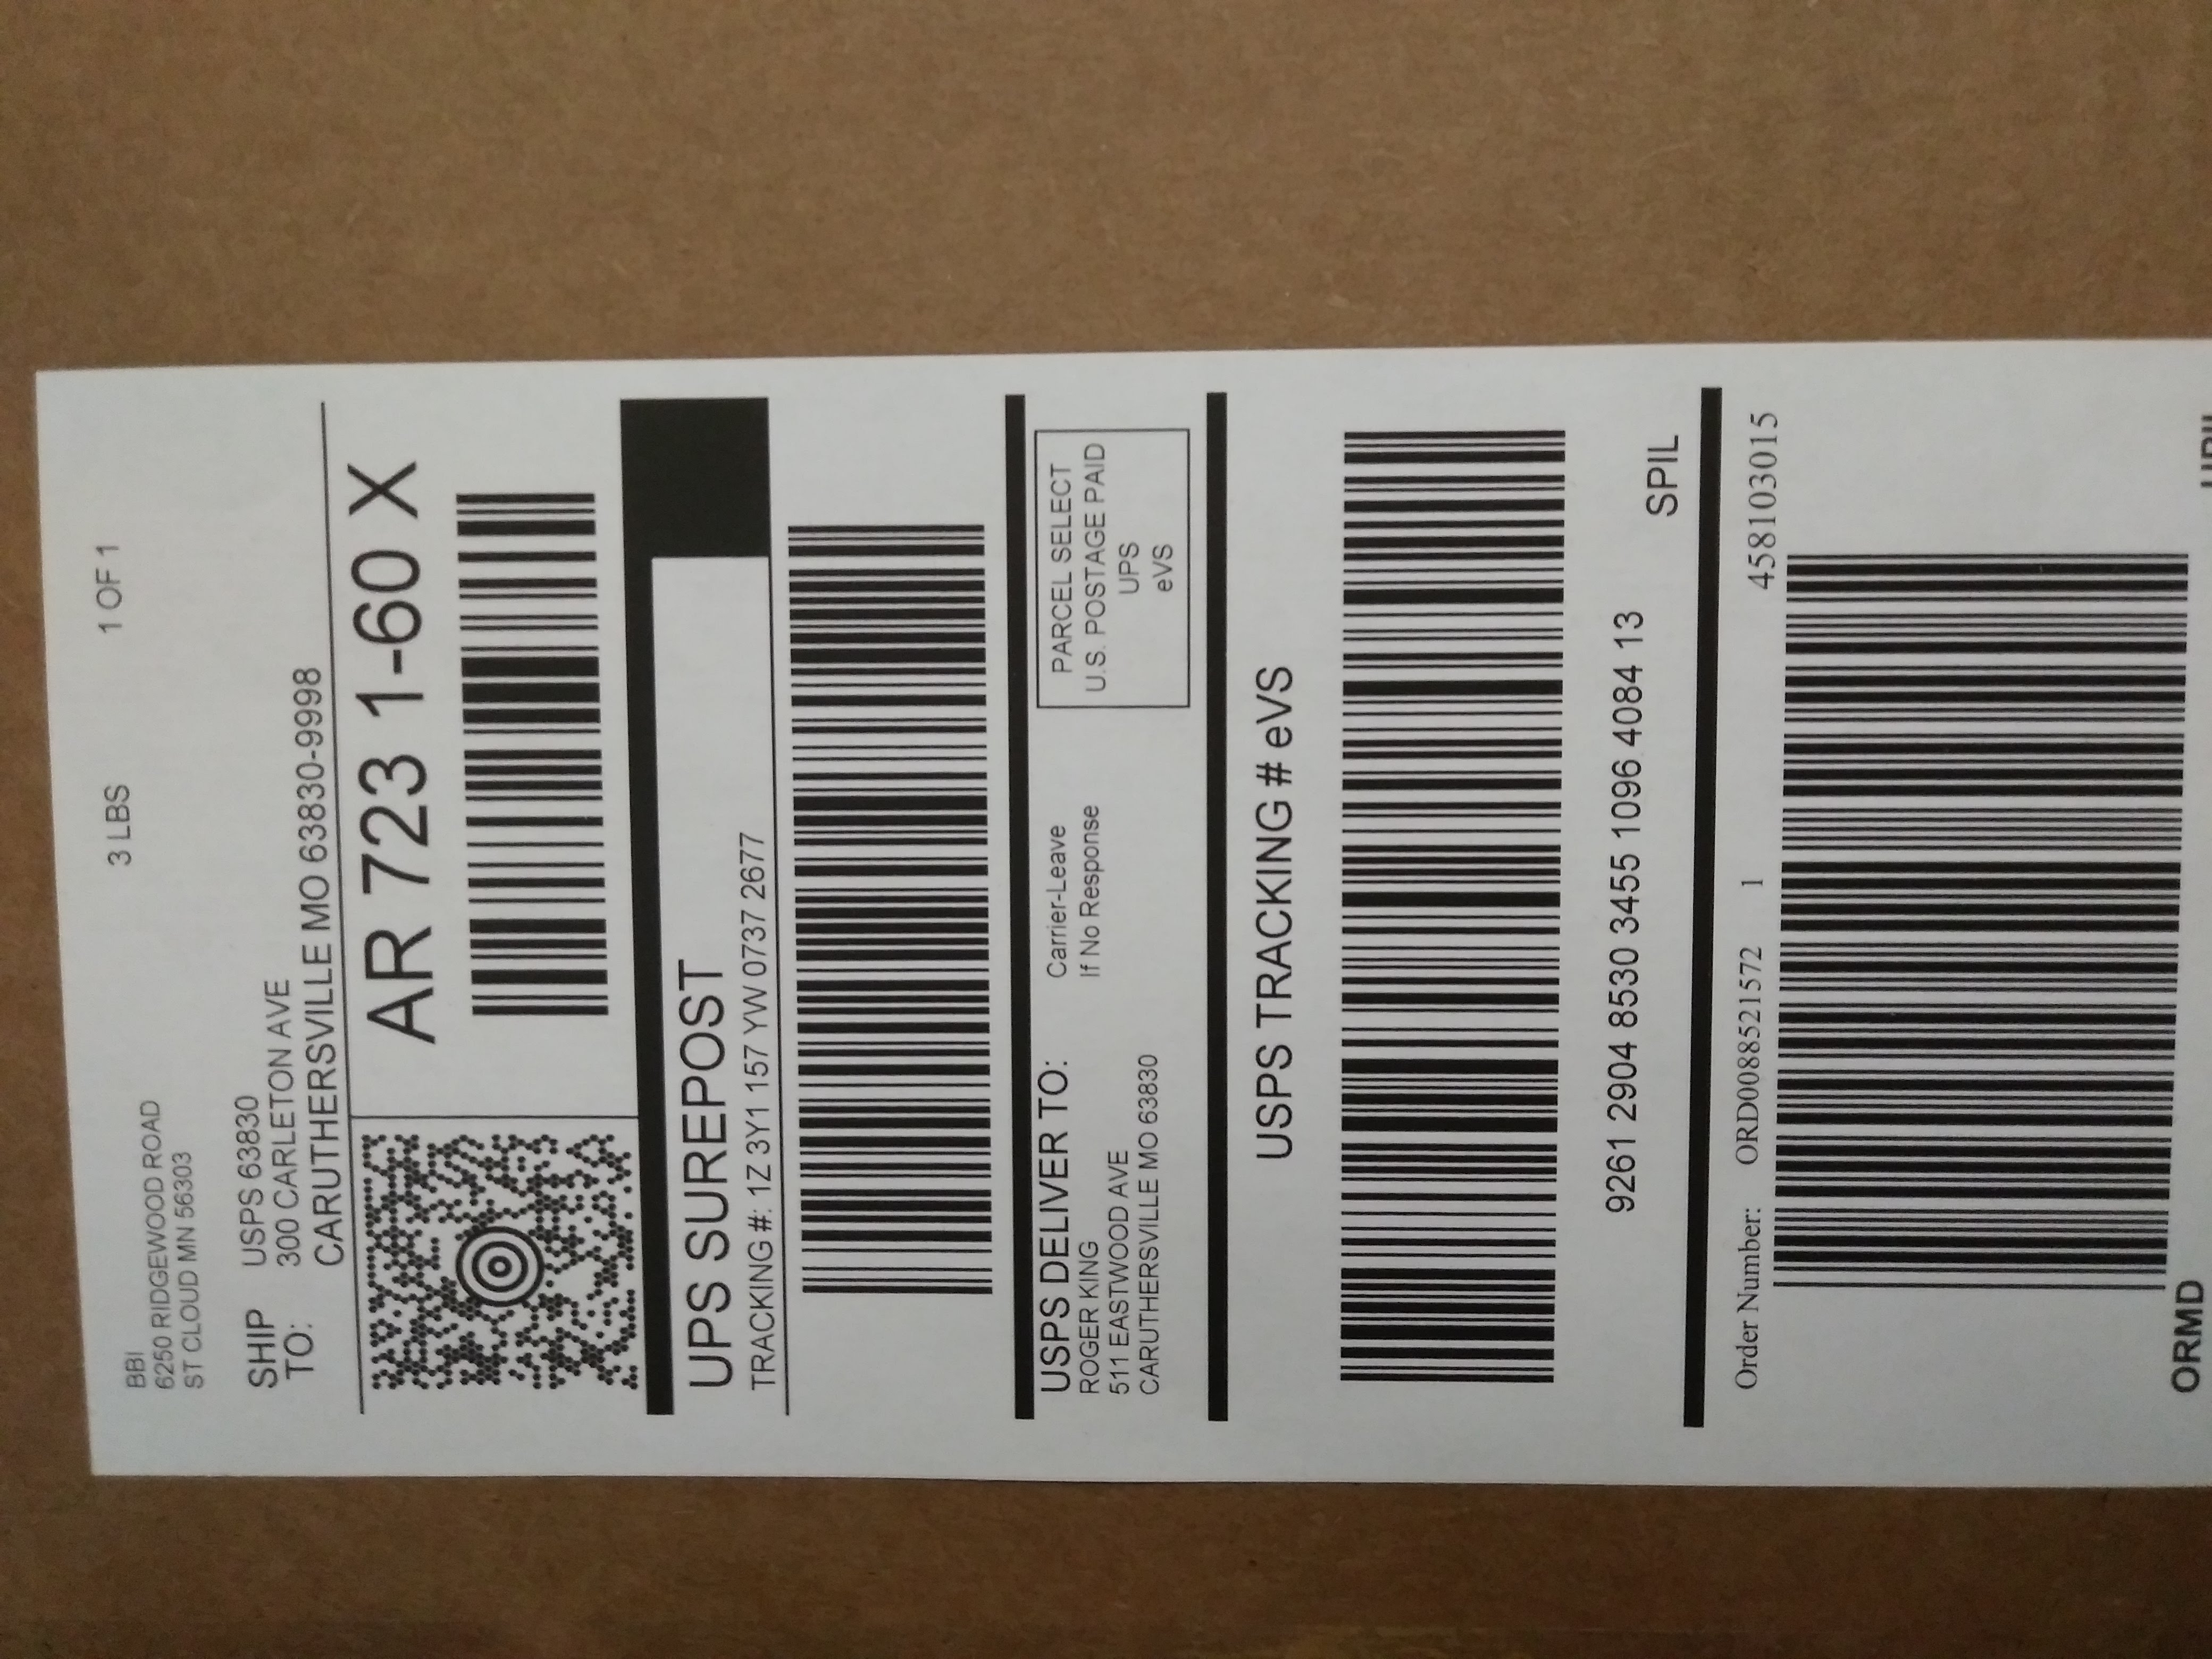
\includegraphics[width=0.7\linewidth]{20171222_184324} 
\caption{MO - AR Discrepancy}
\end{subfigure}
\begin{subfigure}{0.5\textwidth}
\centering
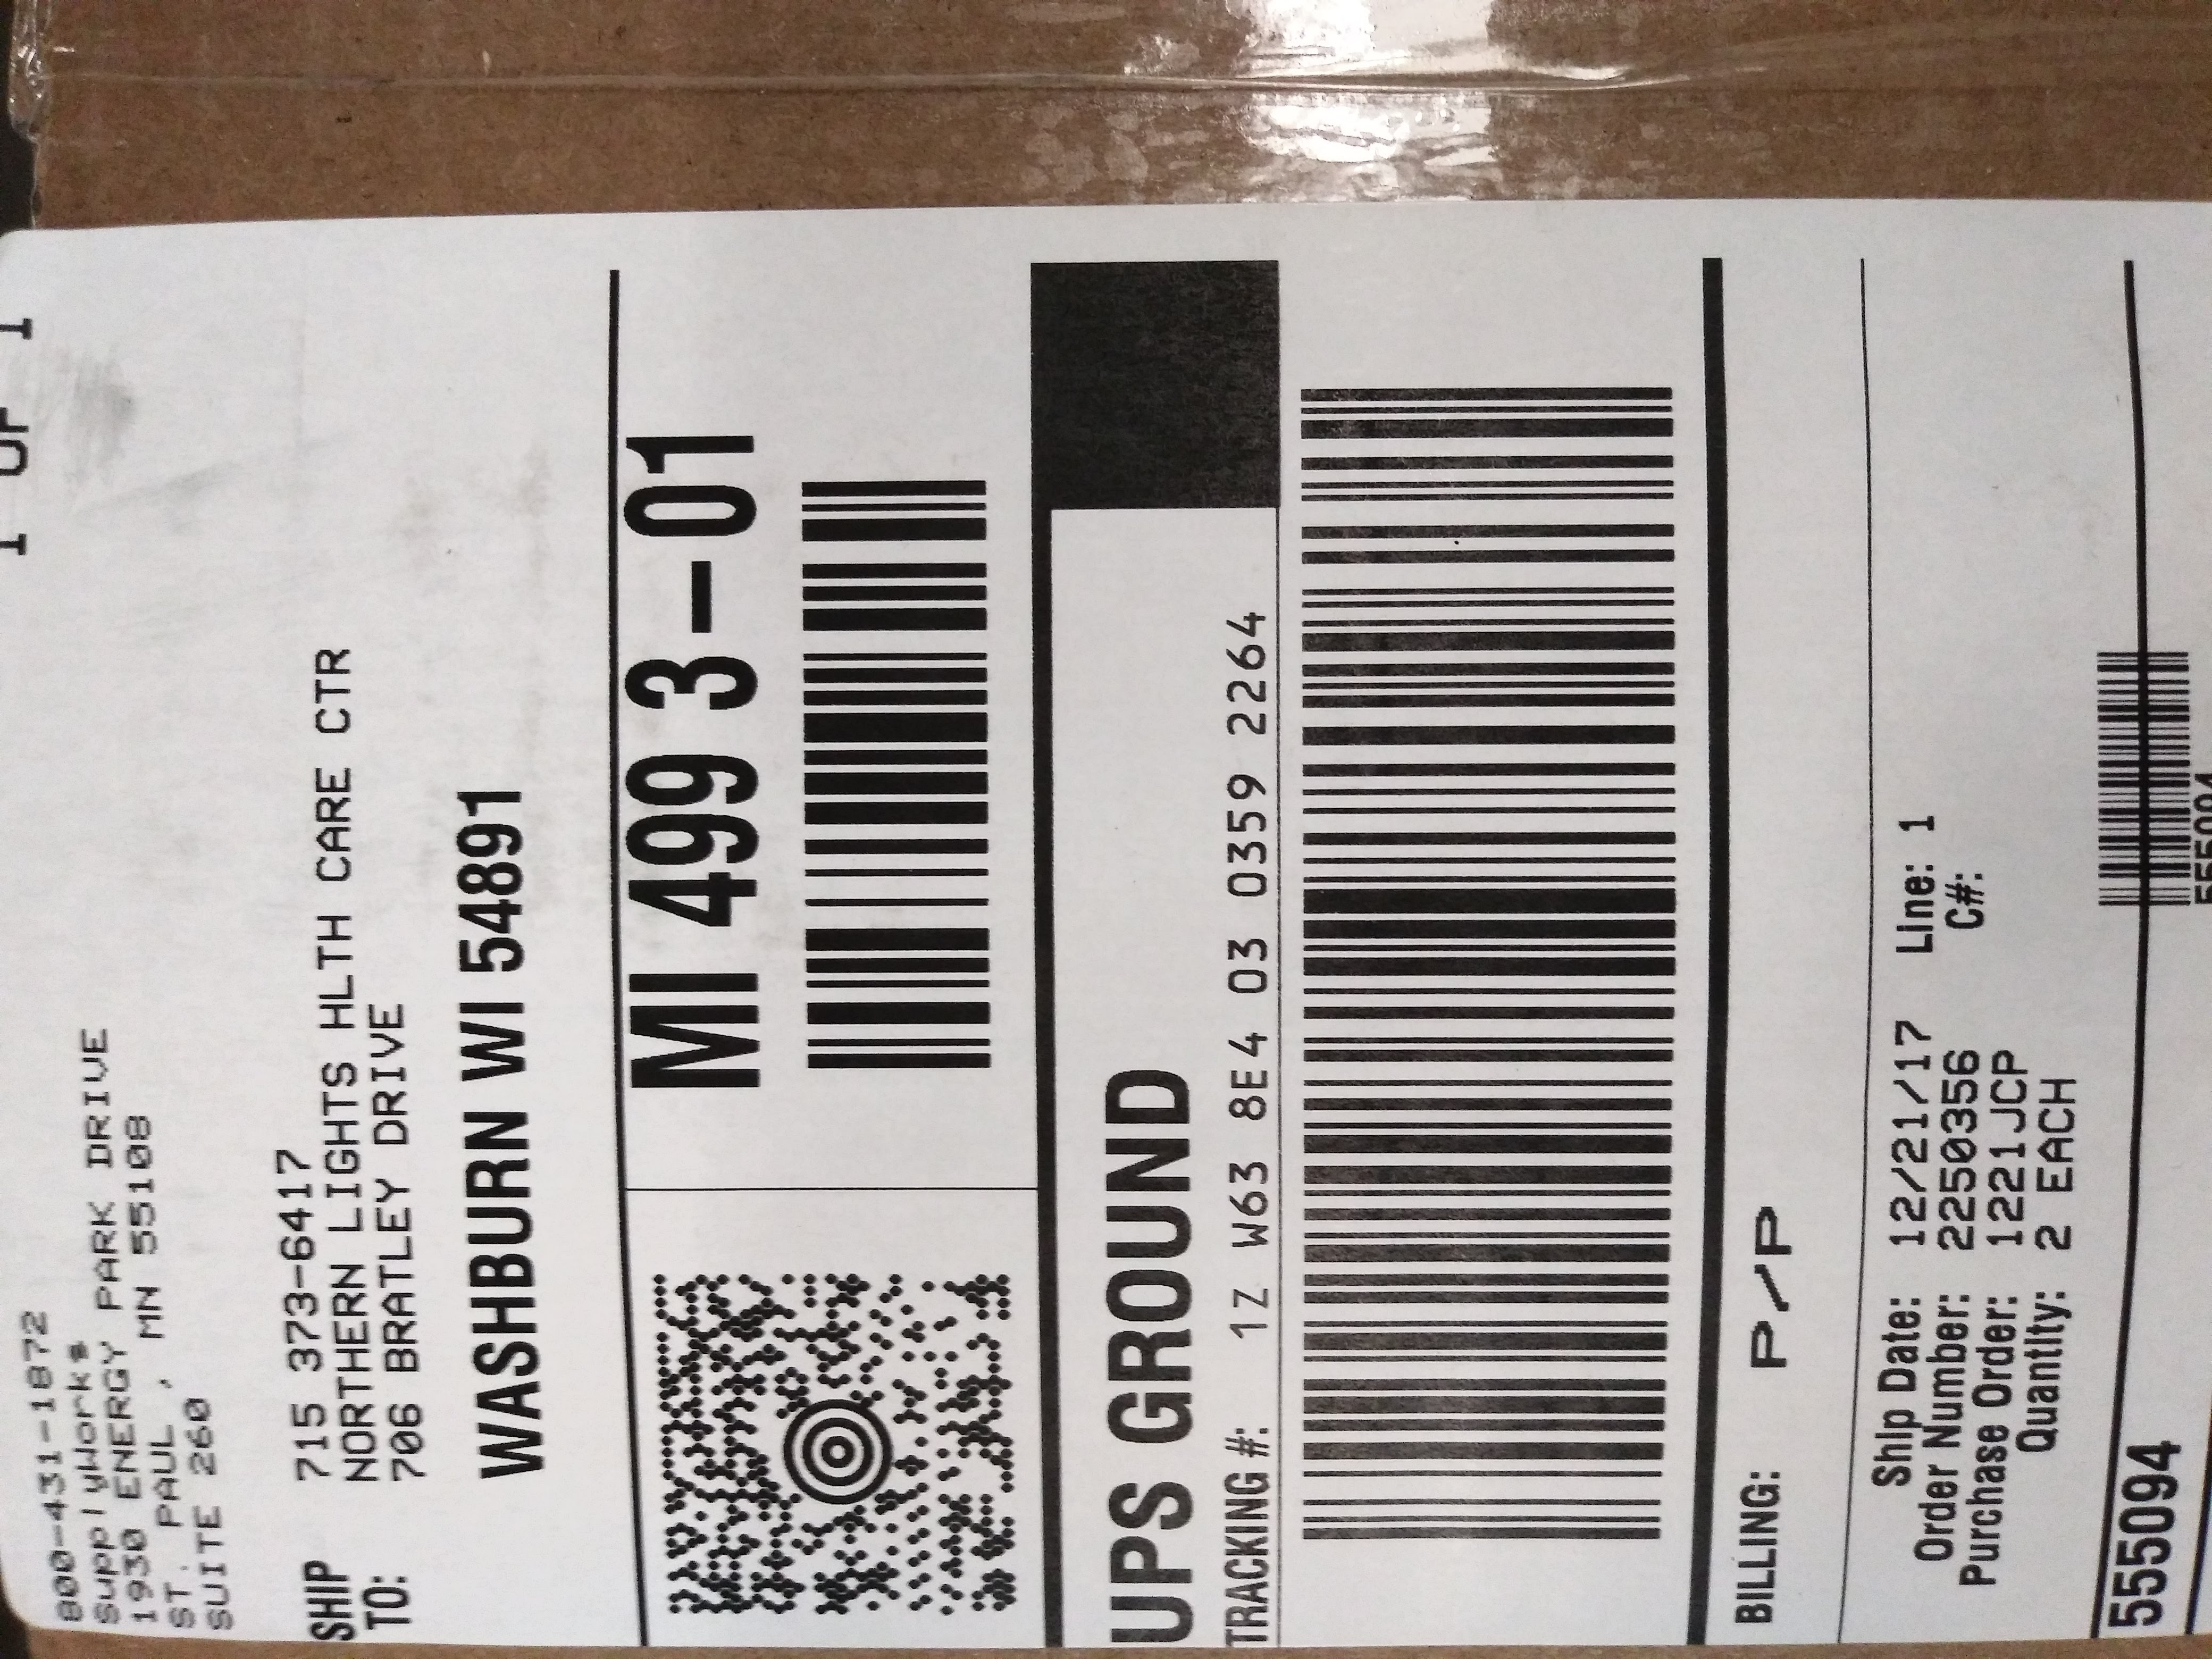
\includegraphics[width=0.7\linewidth]{20171221_200431} 
\caption{MI Exception w/ WI Discrepancy}
\end{subfigure}
\begin{subfigure}{0.5\textwidth}
\centering
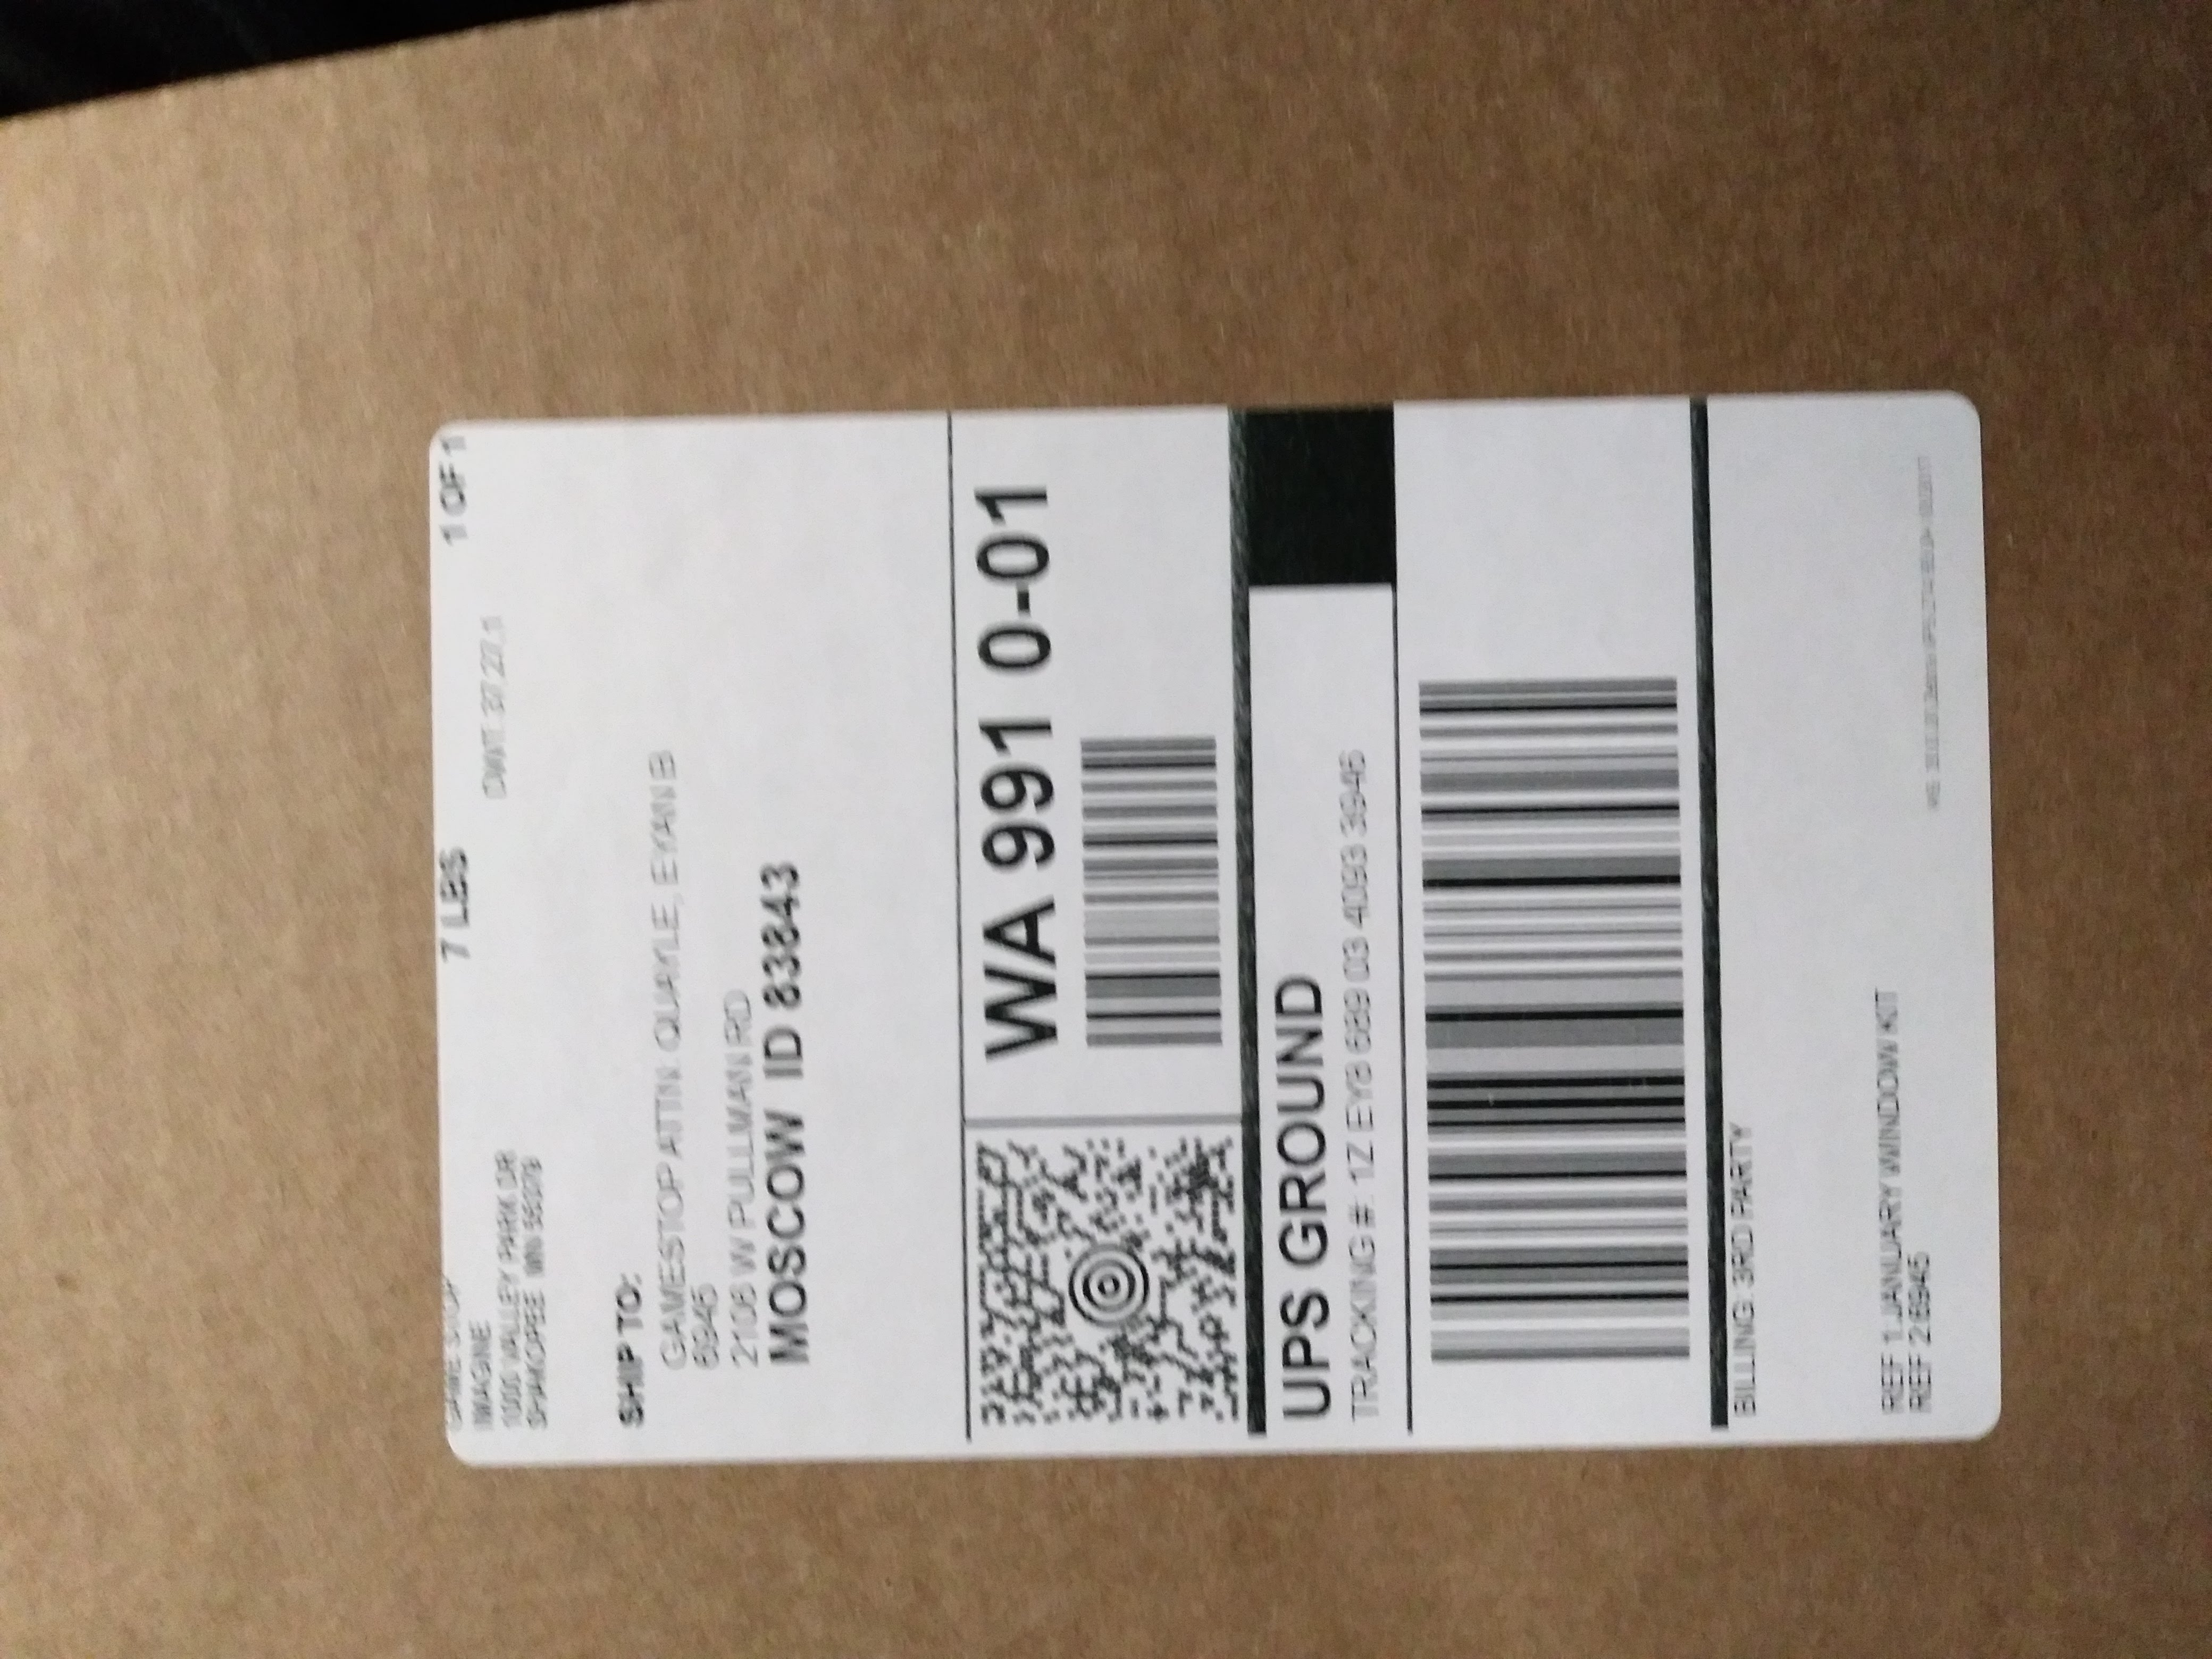
\includegraphics[width=0.7\linewidth]{20171221_180122} 
\caption{ID - WA w/ ID Exception}
\end{subfigure}
\begin{subfigure}{0.5\textwidth}
\centering
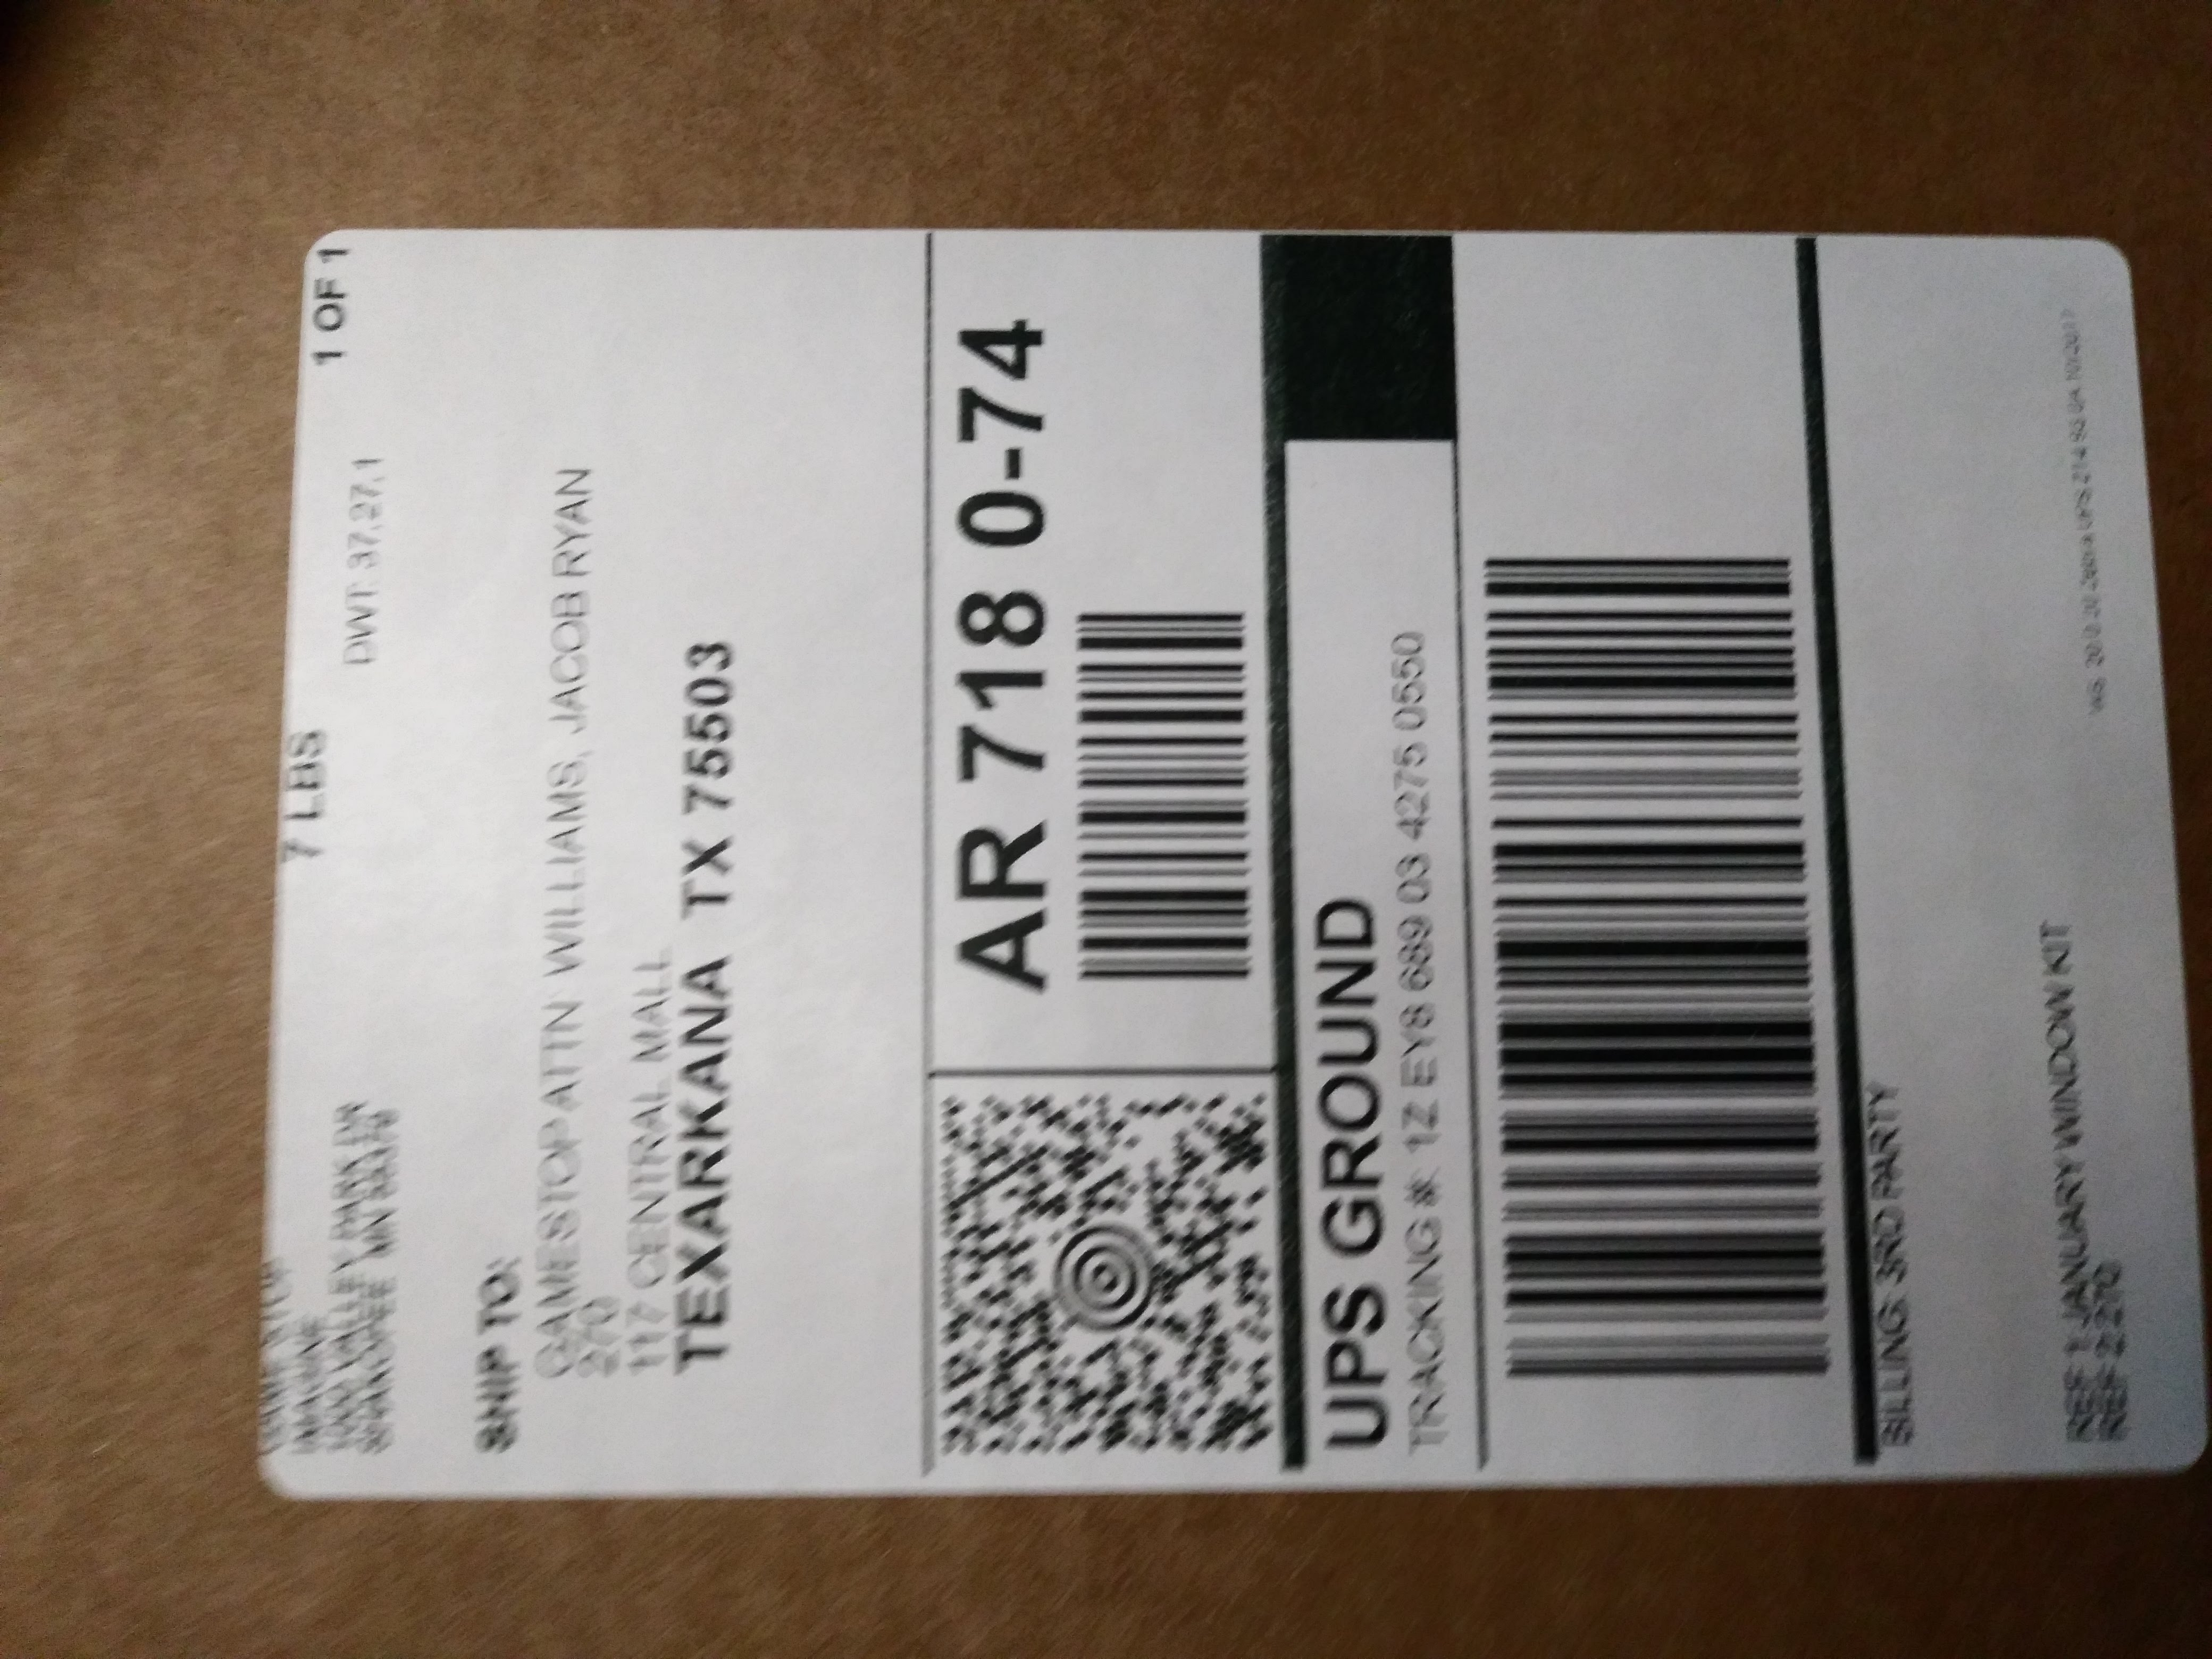
\includegraphics[width=0.7\linewidth]{20171221_173426} 
\caption{TX - AR Discrepancy}
\end{subfigure}
\begin{subfigure}{0.5\textwidth}
\centering
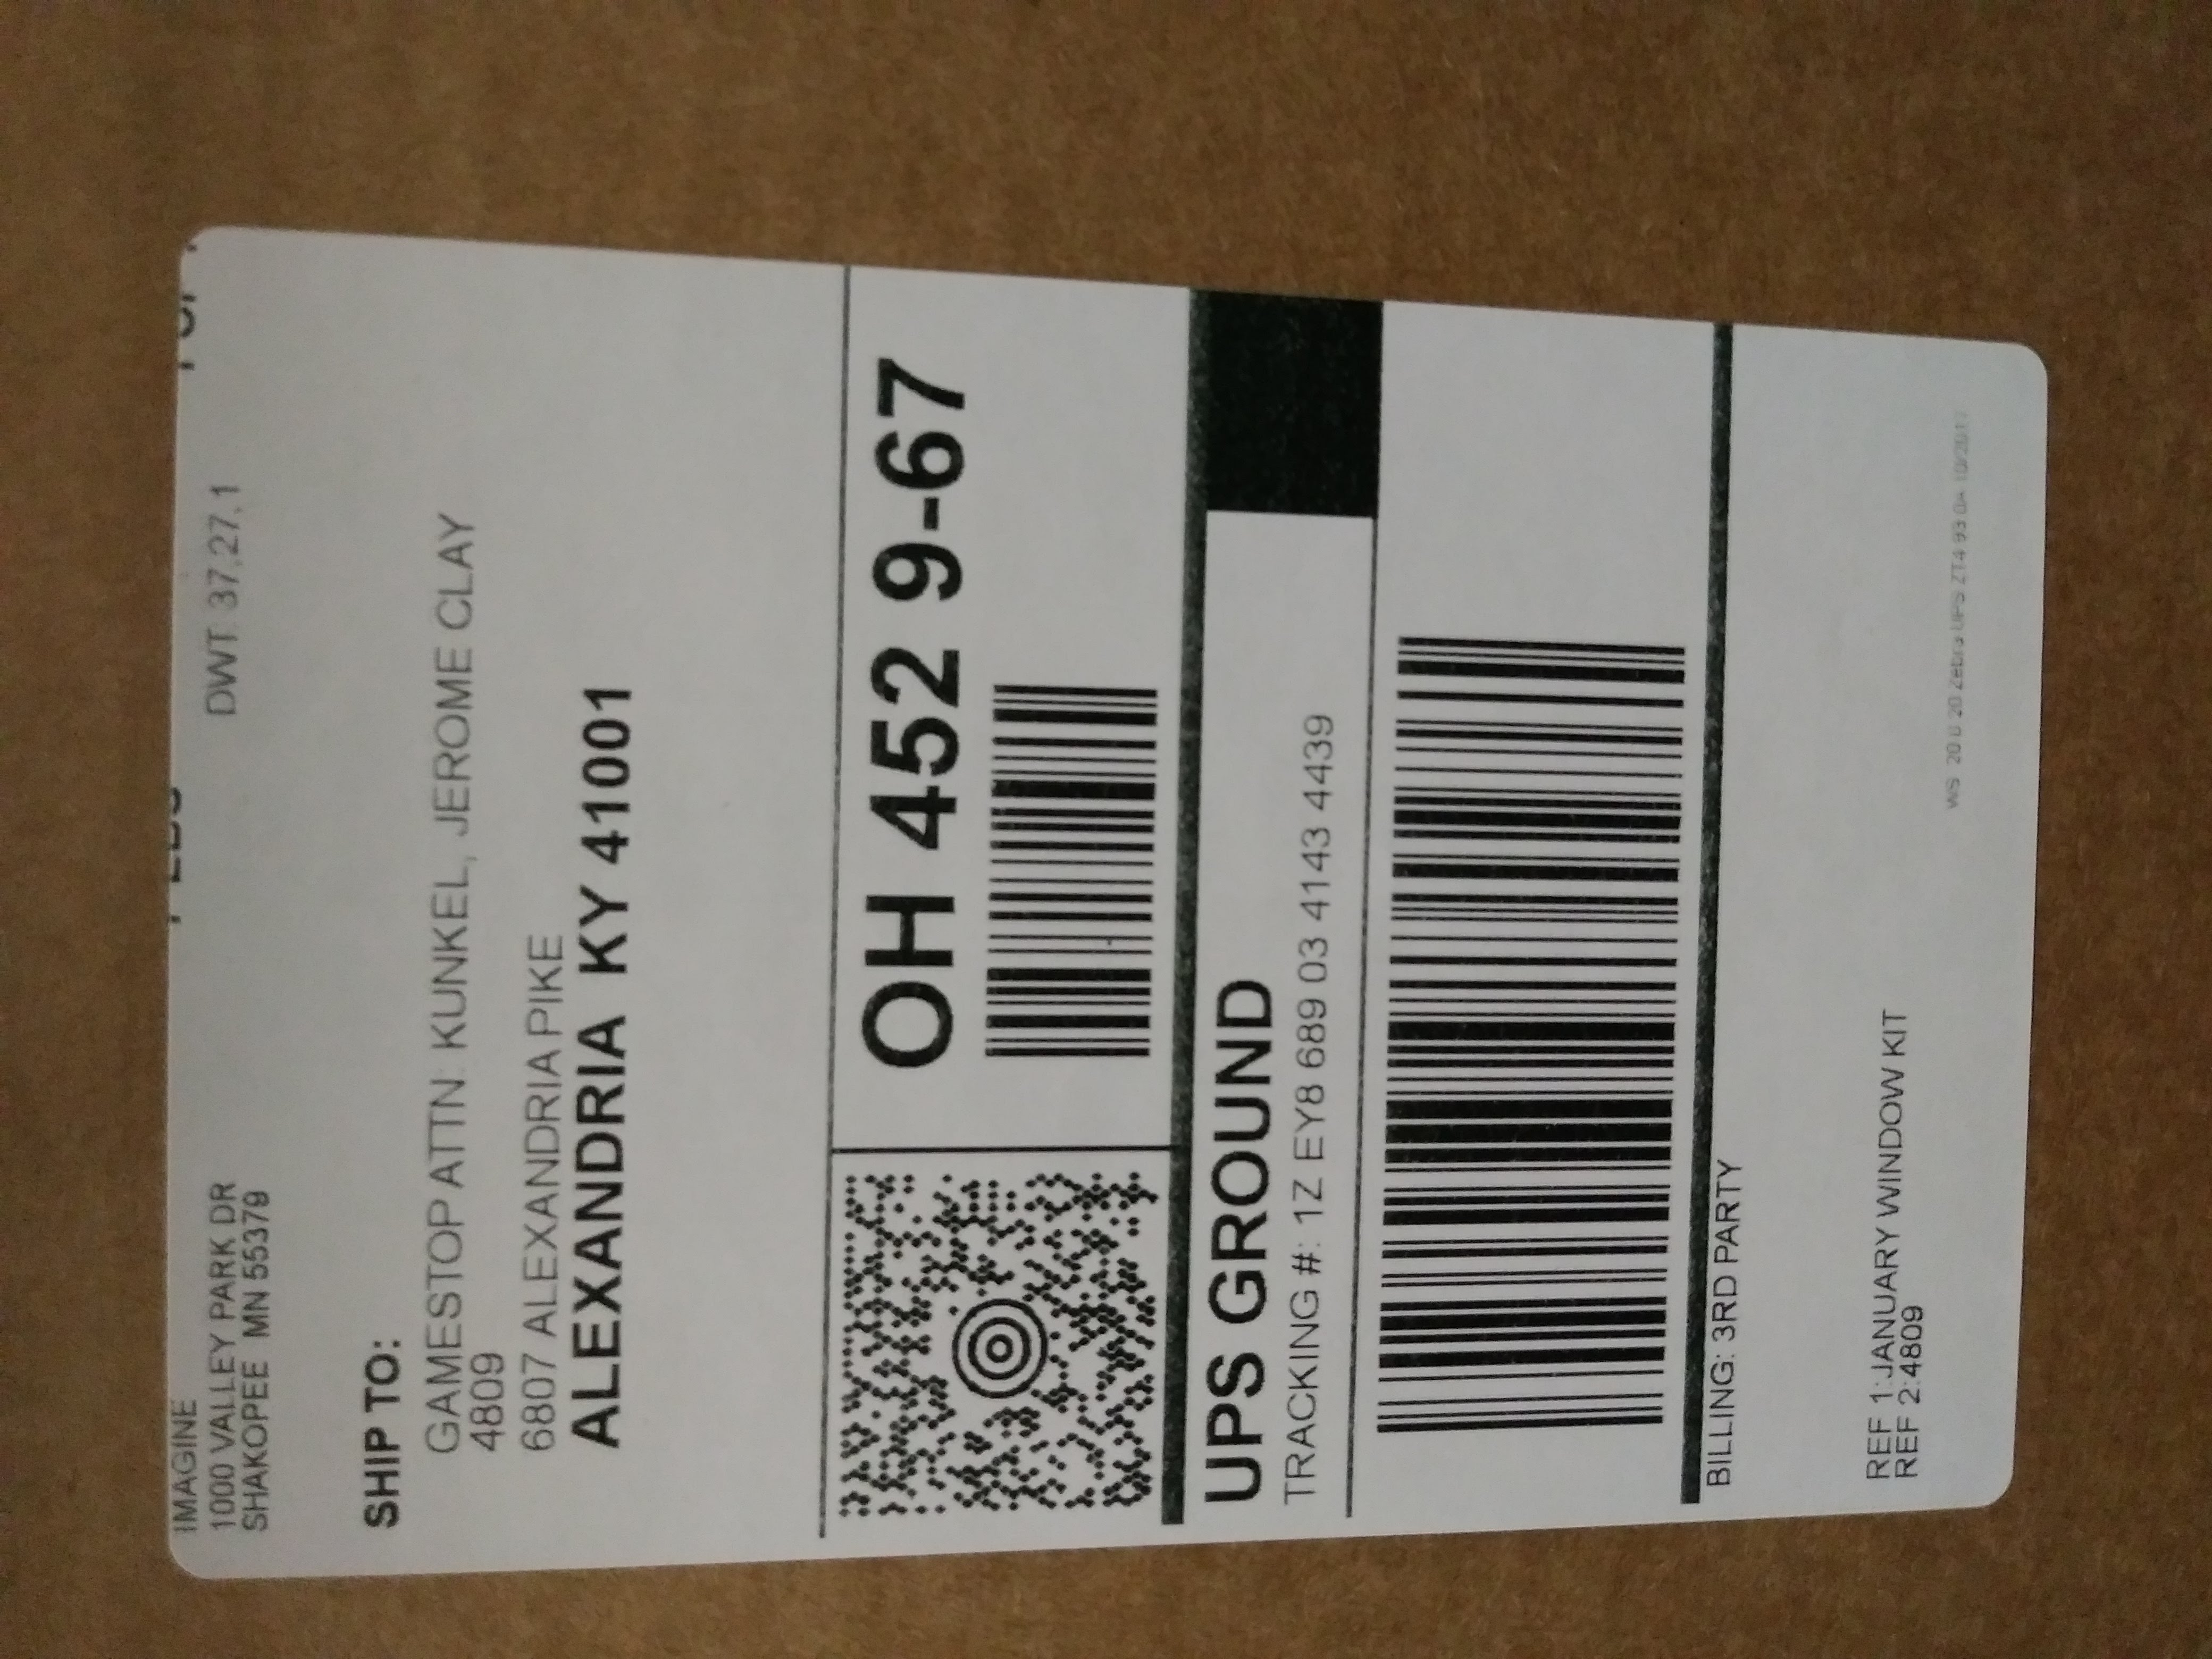
\includegraphics[width=0.7\linewidth]{20171221_171849} 
\caption{KY - OH Discrepancy}
\end{subfigure}

\end{figure}

%%%%%%%%%%%%%%%%%%%%%%%%%%%%%%%%%%%%%%%%%%%%%%%%%%%%%%%%%%%%%%%%%%%%%%%%%%%%%%%
\clearpage
\section{Packaging}

% \subsubsection{Hand to Surface}
% content

\subsection{Smalls}
Containerizing small packages allows UPS to drastically reduce processing time while also protecting the integrity of vulnerable packages. As much volume as possible should be processed by the small sort. 

\begin{itemize}
    \item A small package = 16 x 16 x 7 inches and is 8lb or less. This is larger than you would expect.
    \item Certain packages exceed these dimensions but can be folded and should still be sent to small sort (e.g. a sleeve with clothing)
    \item Certain packages like envelopes or sleeves are especially vulnerable to damage or loss during the shipping process. Extra emphasis should be placed on getting these to small sort. 
    \item If small packages arrive in a tote then they should be kept in the tote going to small sort.
\end{itemize}

\begin{figure}[H]
\begin{subfigure}{0.5\textwidth}
\centering
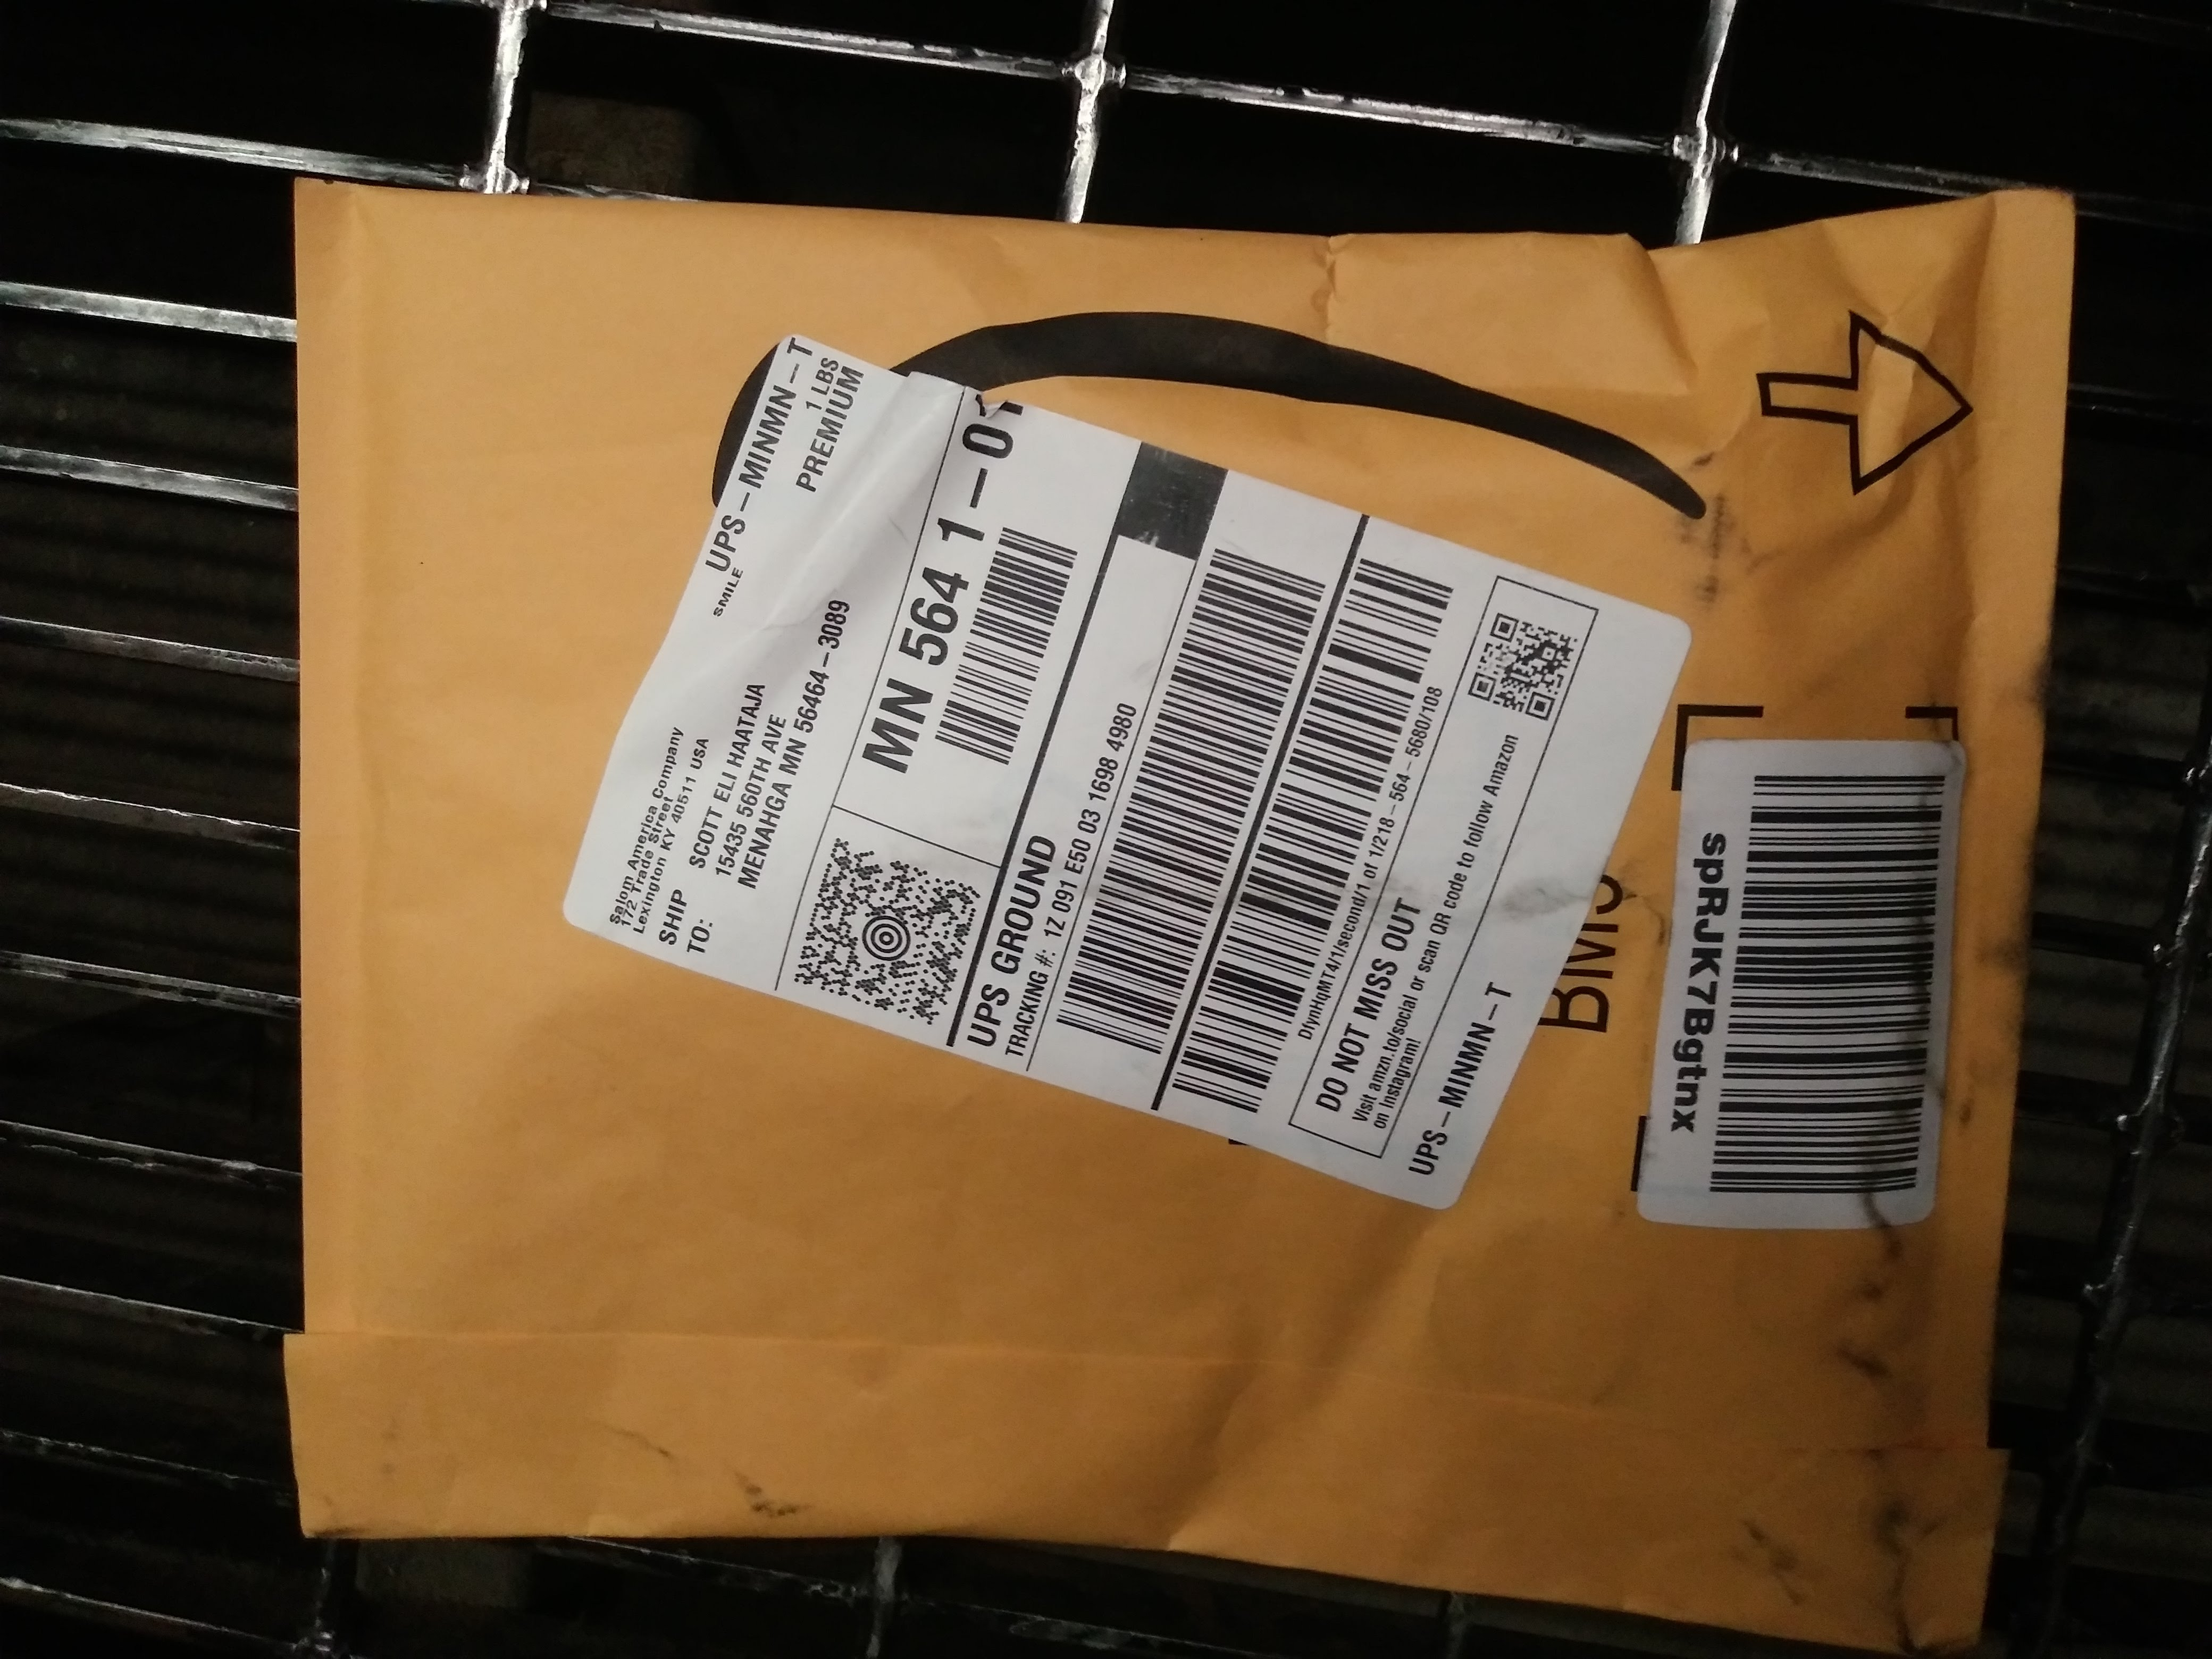
\includegraphics[width=0.7\textwidth]{20171221_155646.jpg} 
\caption{Paper Envelopes}
\end{subfigure}
\hfill
\begin{subfigure}{0.5\textwidth}
\centering
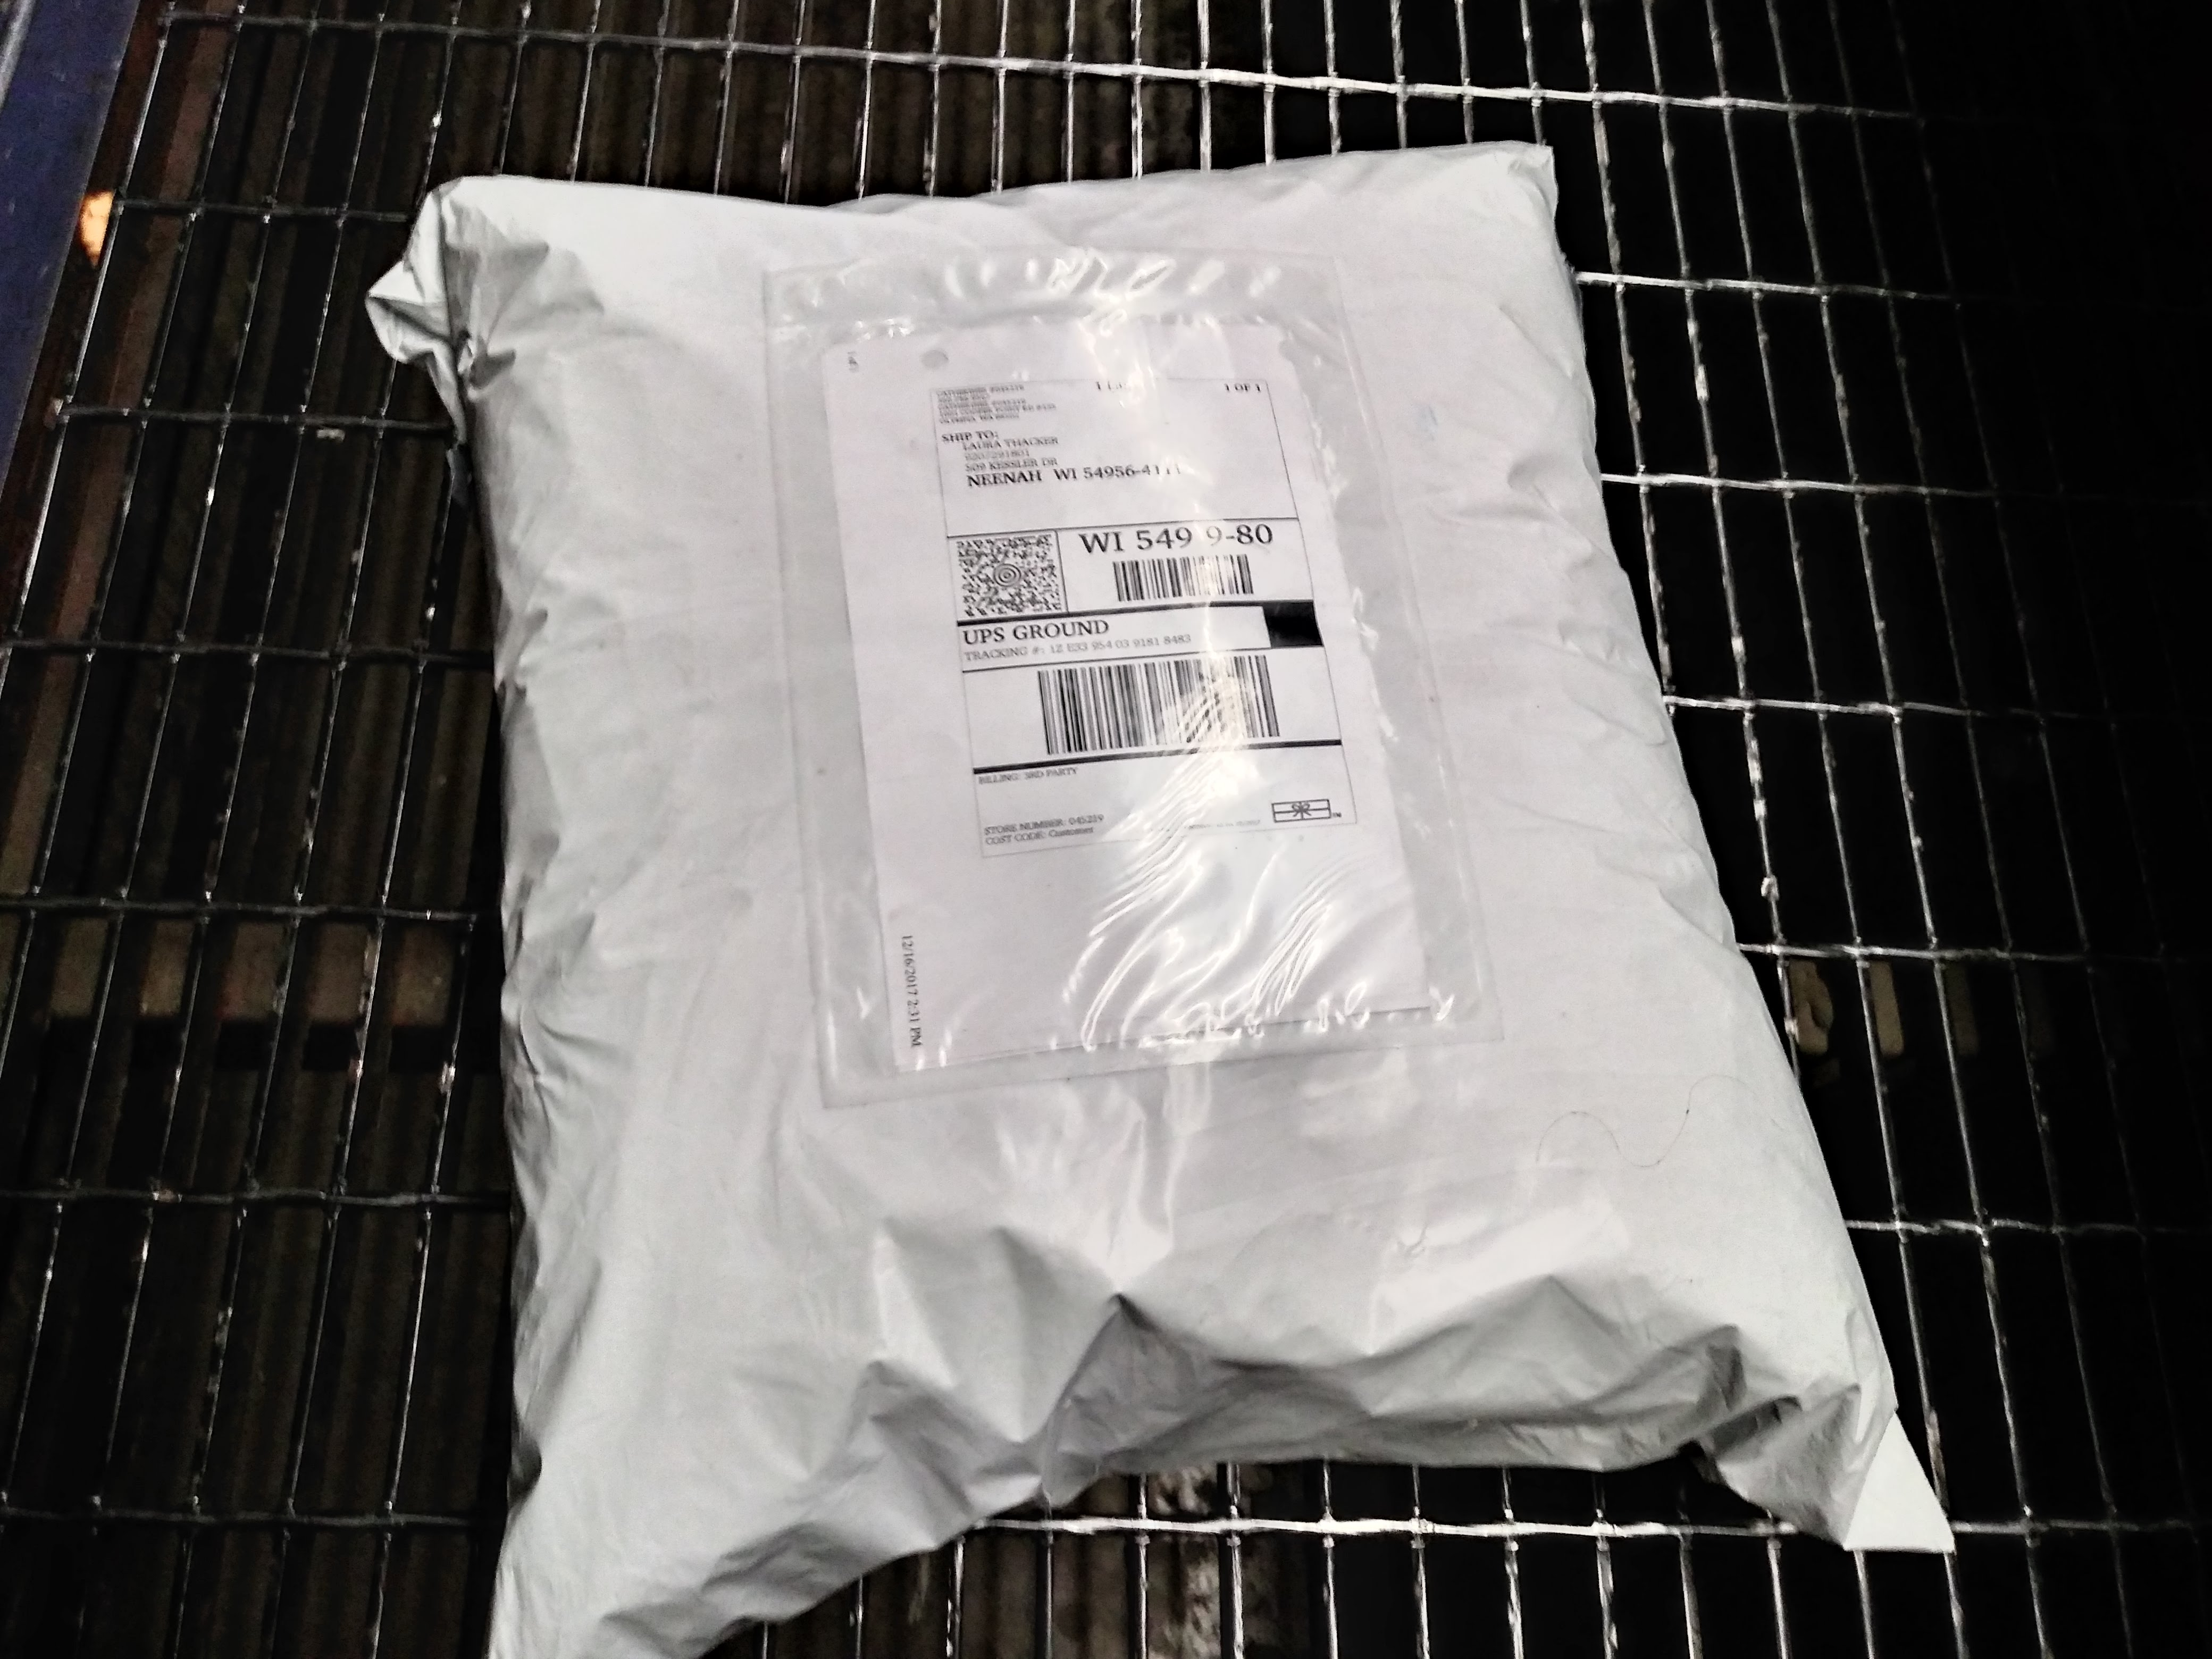
\includegraphics[width=0.7\textwidth]{20171221_171525_HDR.jpg} 
\caption{Plastic Envelopes}
\end{subfigure}
\hfill
\begin{subfigure}{0.5\textwidth}
\centering
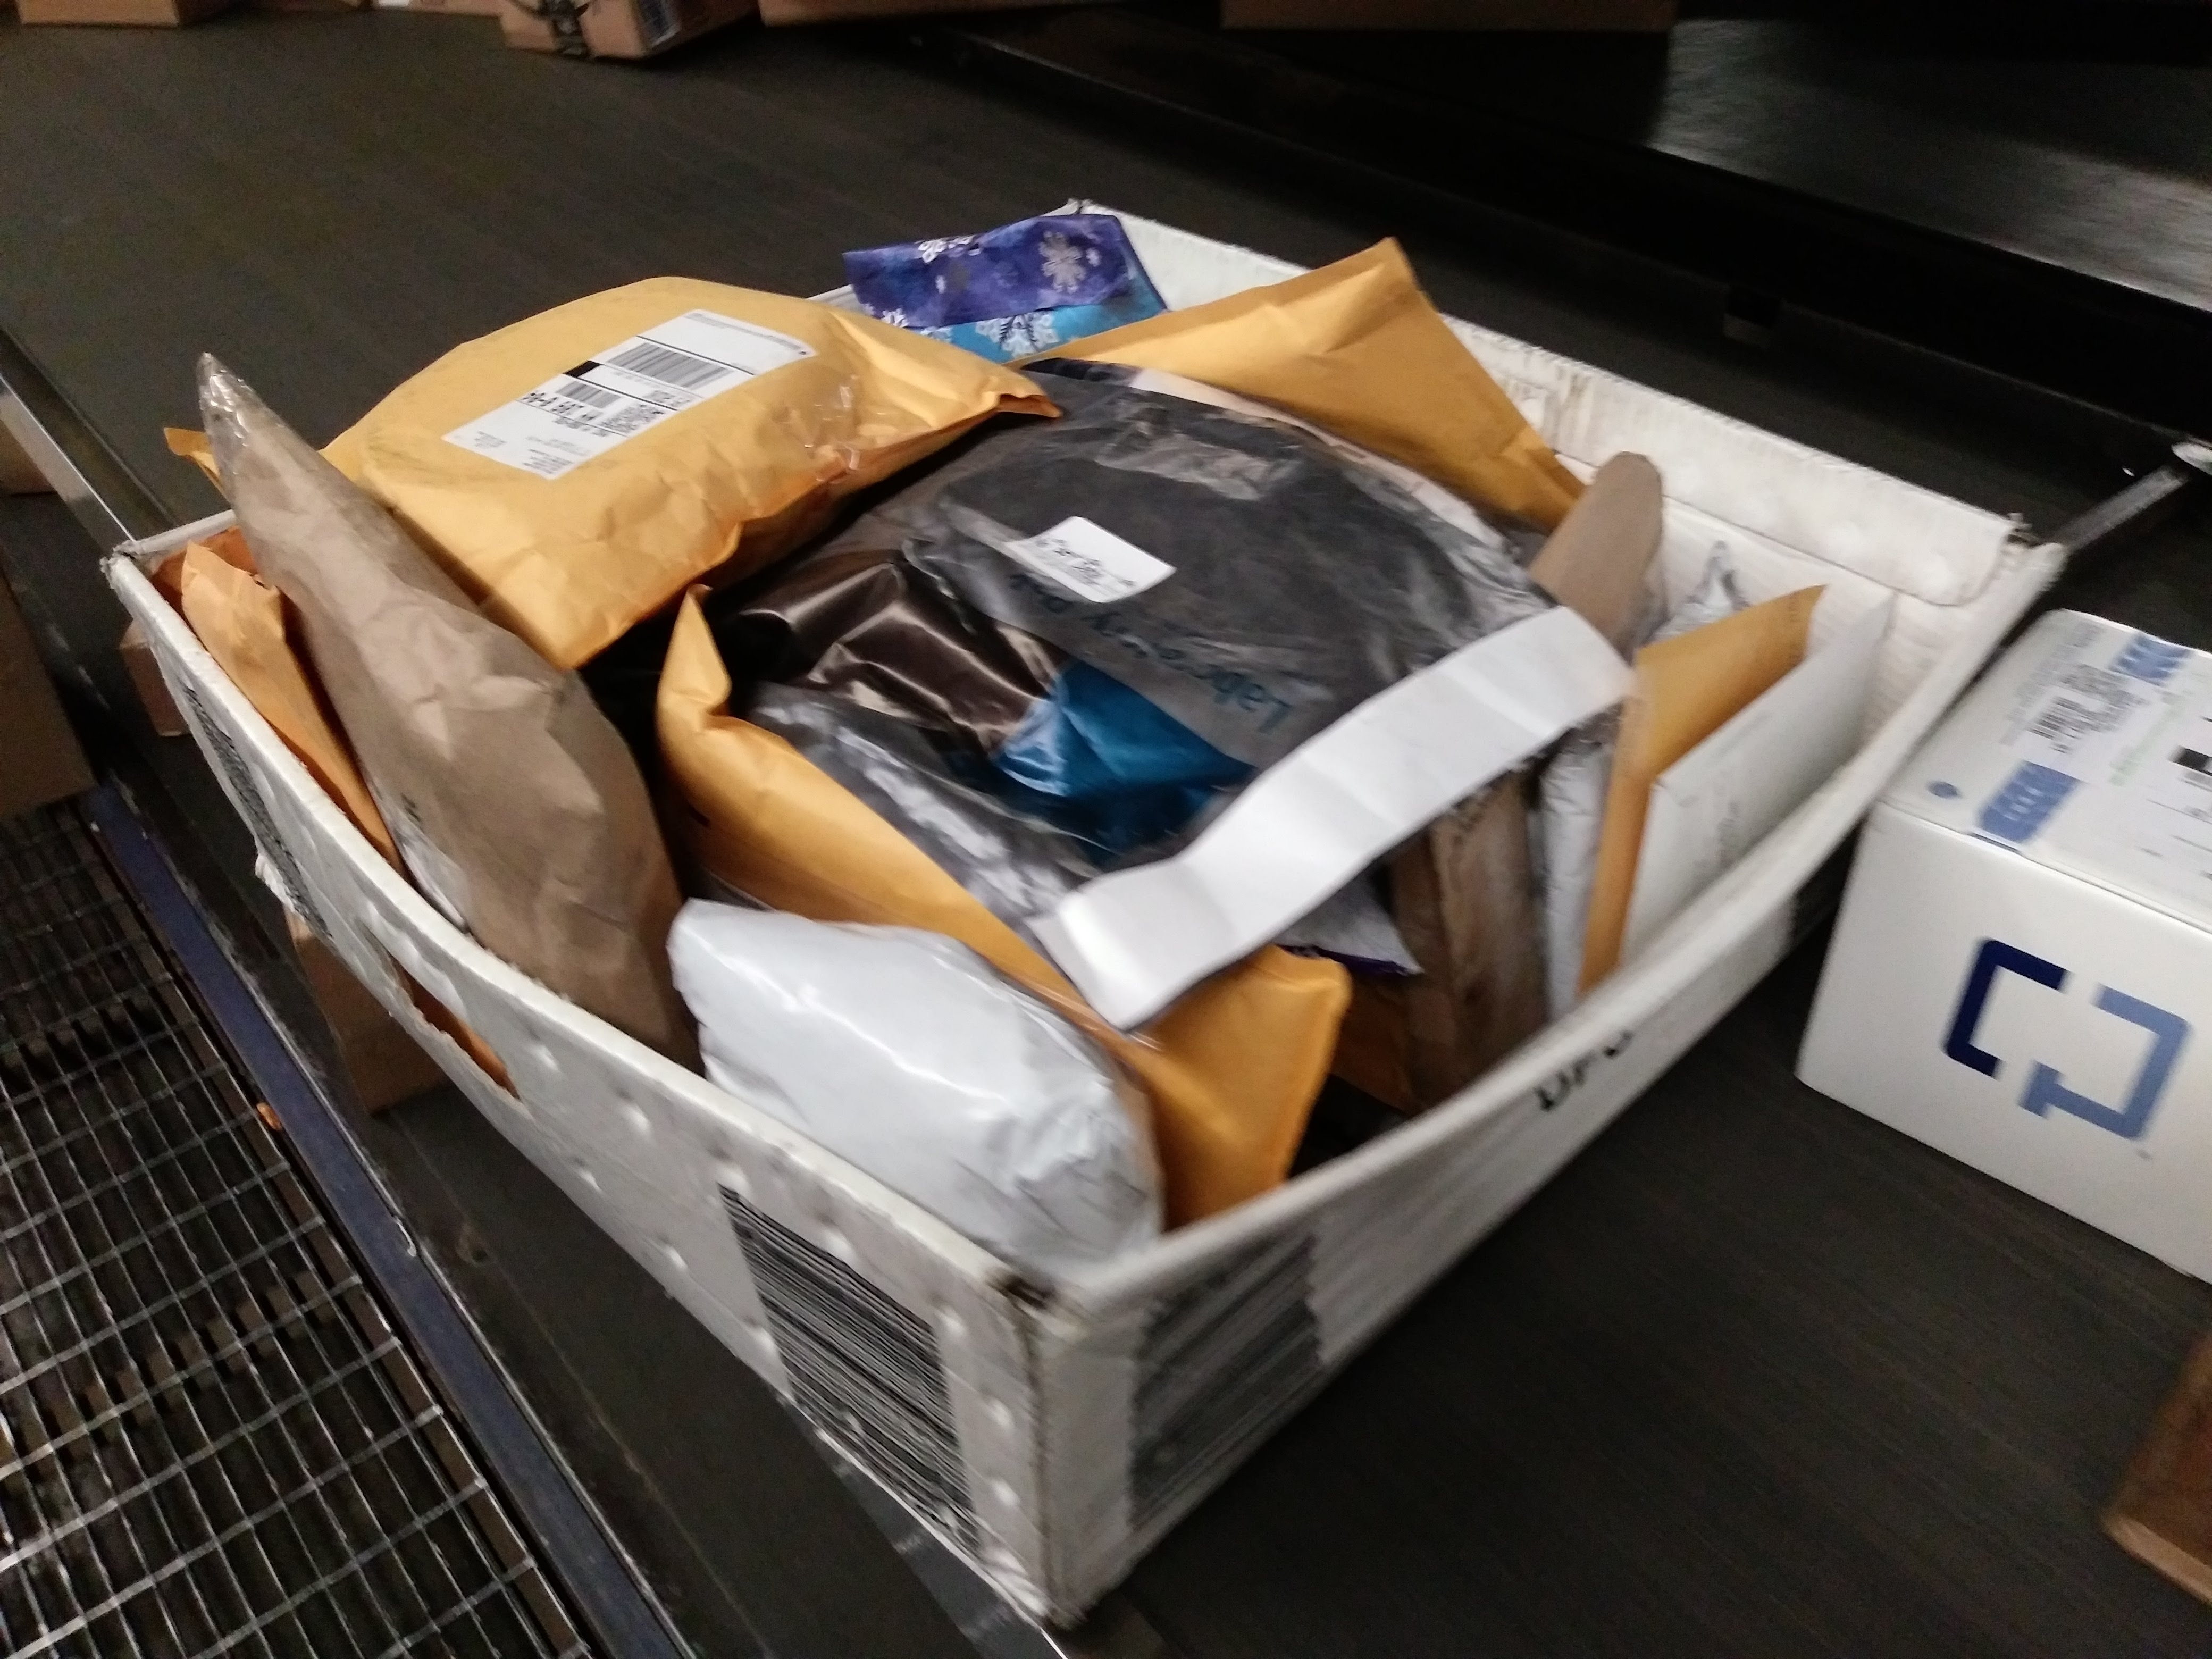
\includegraphics[width=0.7\textwidth]{20171221_163150.jpg} 
\caption{Smalls Totes}
\end{subfigure}
\end{figure}
\clearpage
\subsection{Damages}

\subsubsection{Retape/Rewrap}
An unfortunate reality of being a package courier is that some boxes will come open during the shipping process. There are two classes of open boxes: the ones that need to be retaped and the ones that need to be rewrapped. 

\begin{itemize}
    \item Set retapes and rewraps out of the way while sorting.
    \item Boxes that retain their structure and integrity but are open to content loss should be retaped.
    \item Boxes that cannot be salvaged or that contain leaked content should be sent to the rewrap department.
\end{itemize}

\begin{figure}[H]
\begin{subfigure}{0.5\textwidth}
\centering
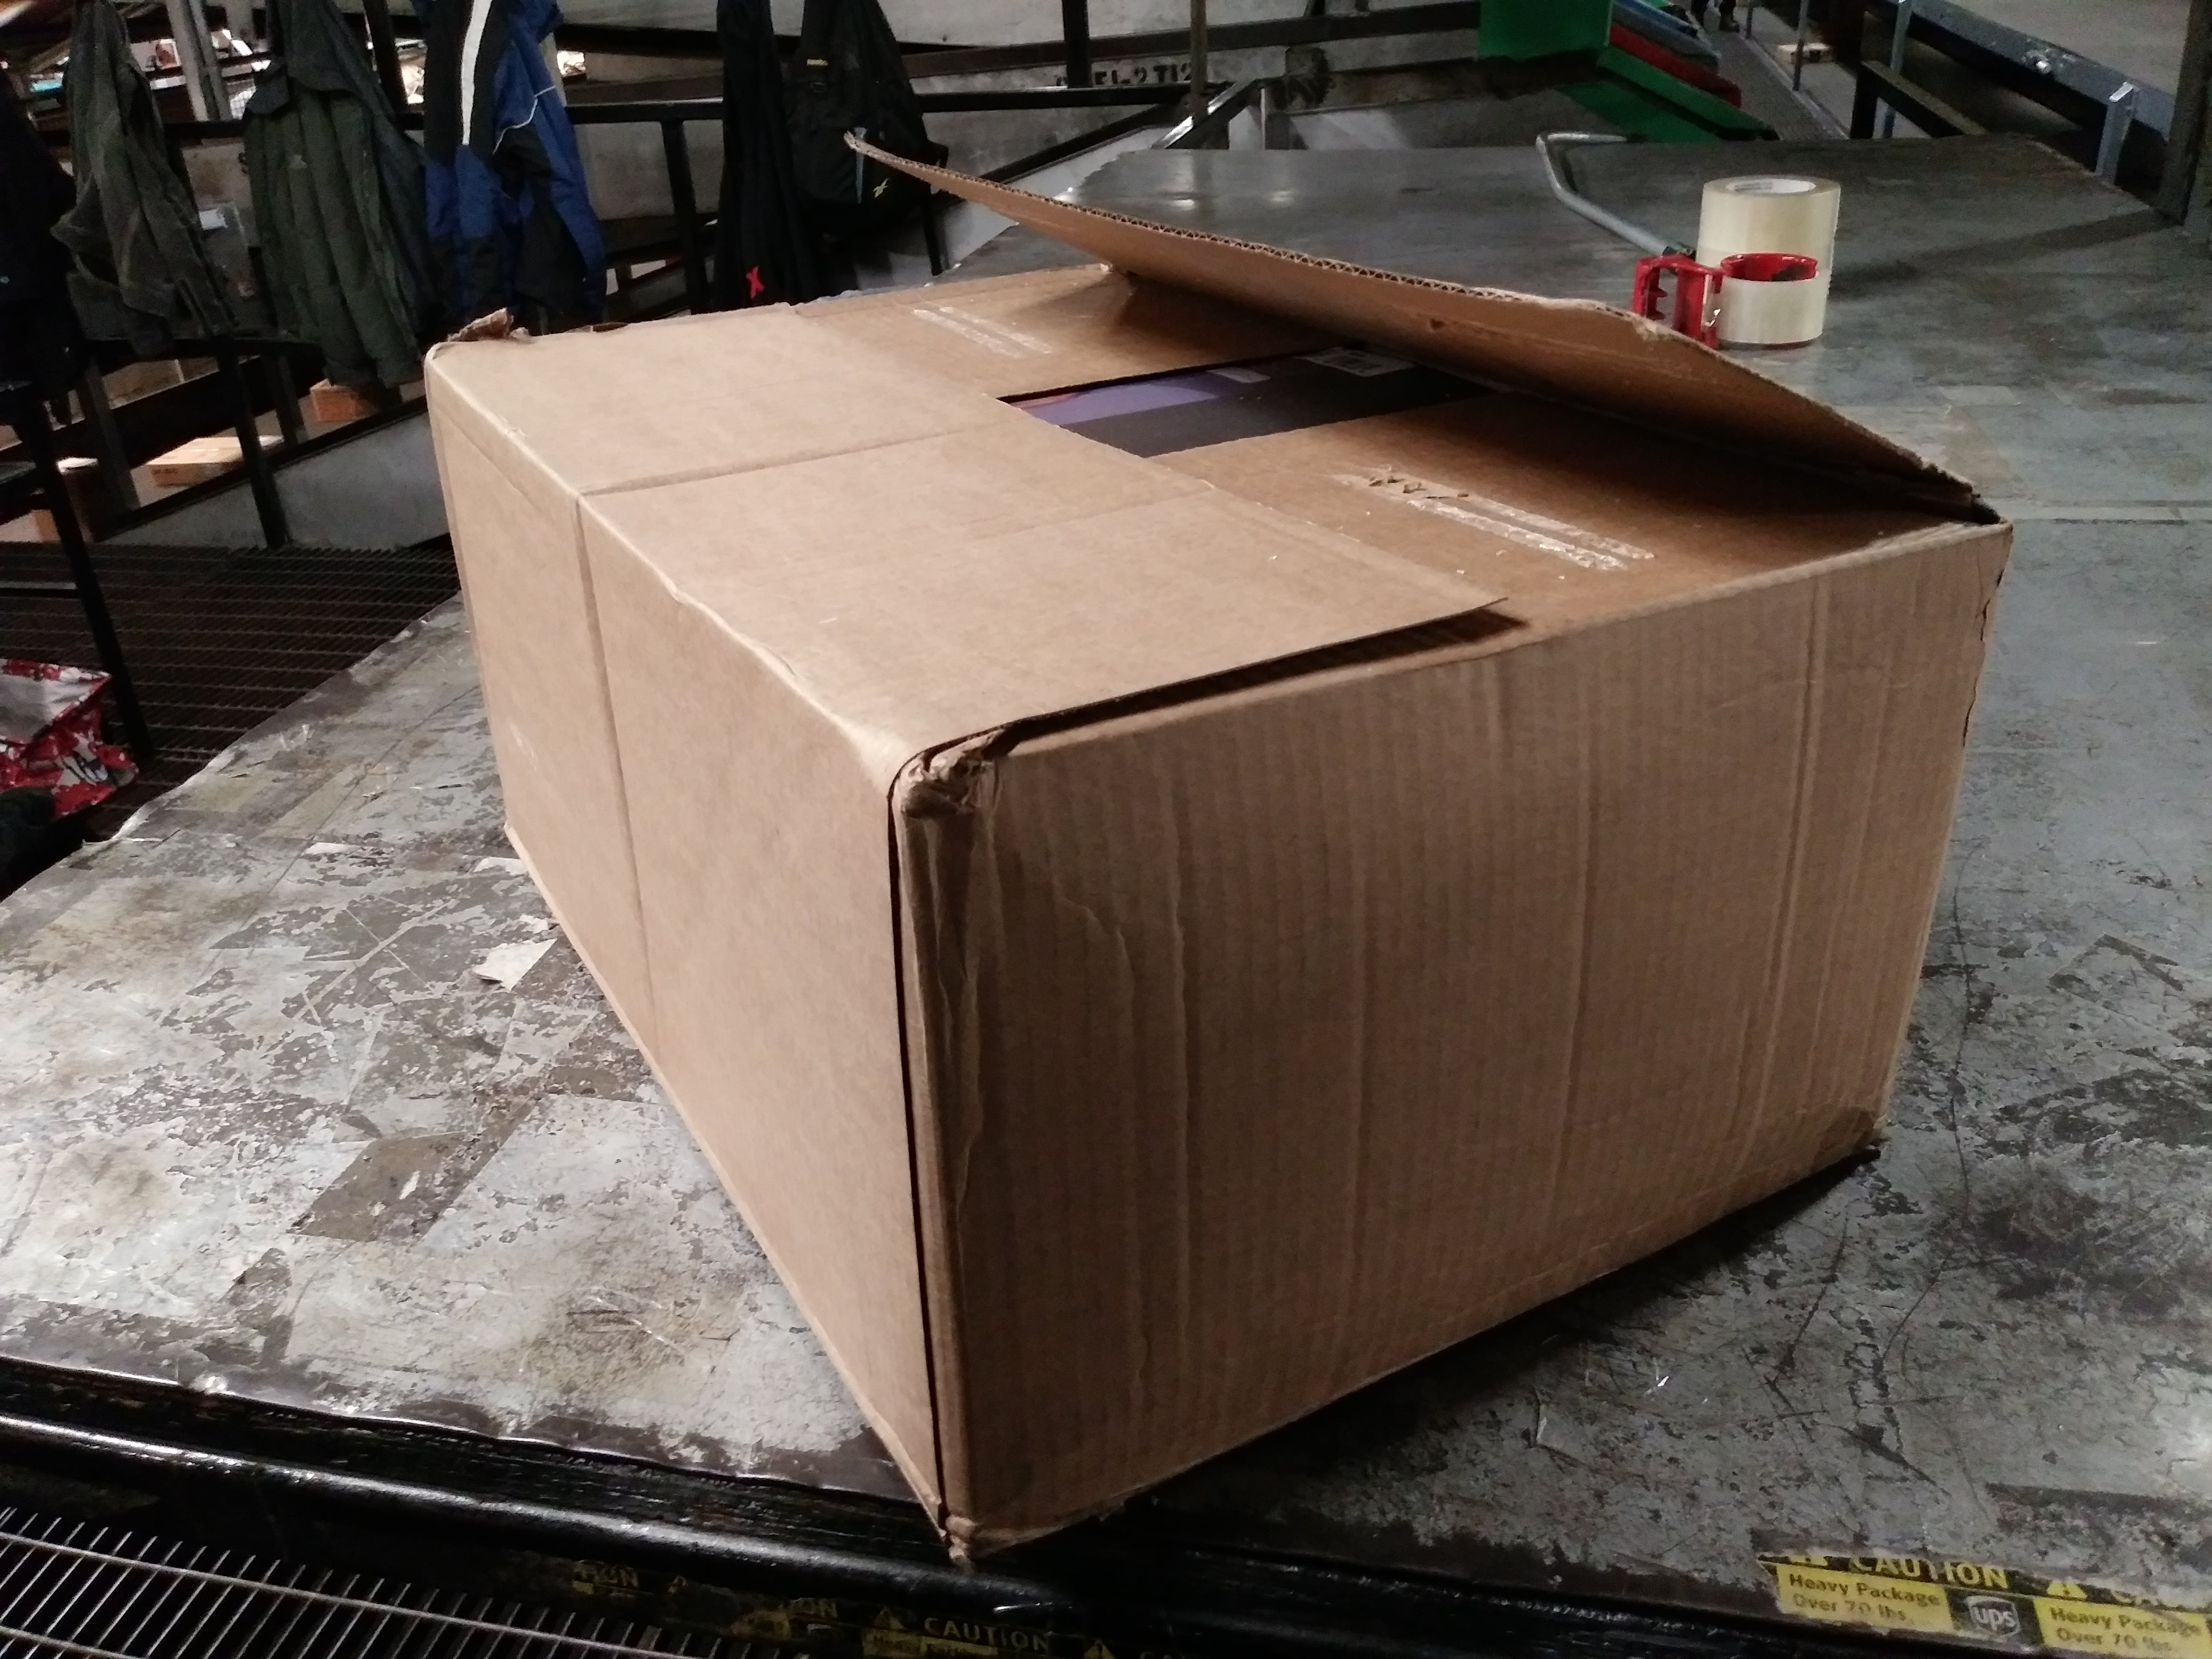
\includegraphics[width=0.7\linewidth]{20171221_160603} 
\caption{Retape package}
\end{subfigure}
\begin{subfigure}{0.5\textwidth}
\centering
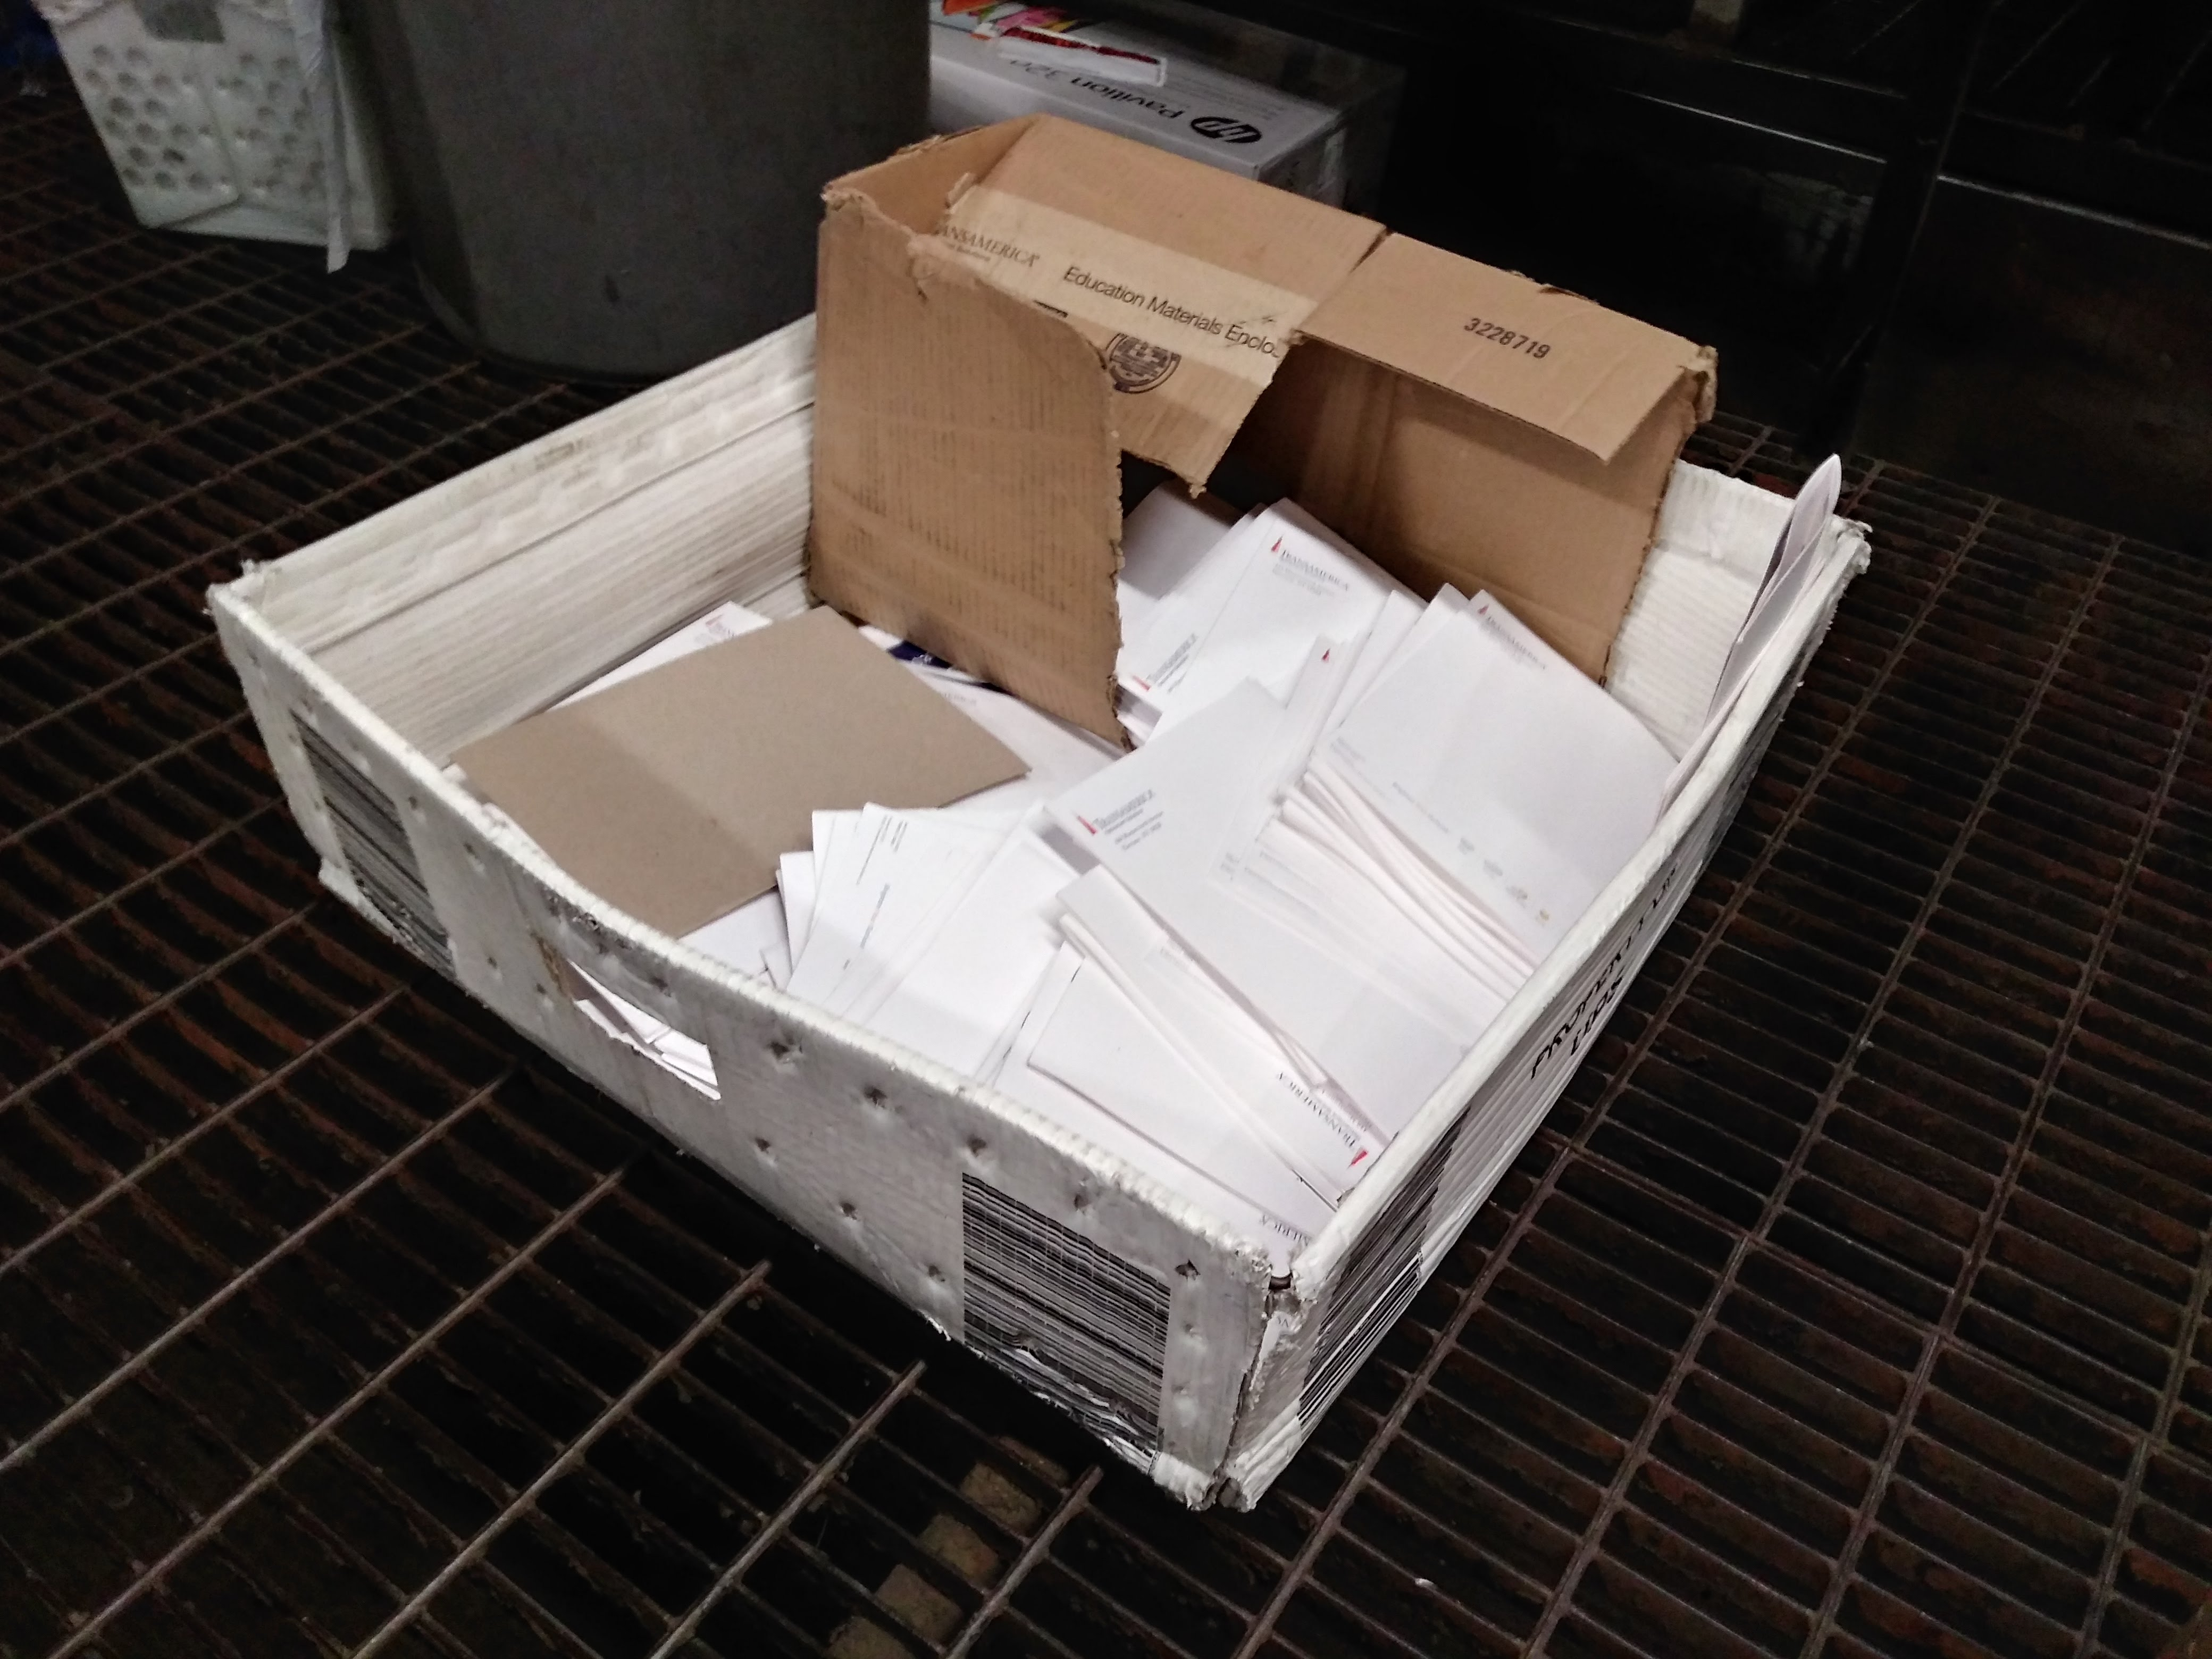
\includegraphics[width=0.7\linewidth]{20171222_013019_HDR}
\caption{Rewrap}
\end{subfigure}
\end{figure}

\subsubsection{Leaking Packages}
Another unfortunate and possibly dangerous case is one where liquid or powder contents escape their containment within the package. This is a serious issue and should be dealt with immediately. 

\begin{itemize}
    \item Notify your supervisor immediately.
    \item Even if the package does not contain hazmat labels you should still treat it as hazardous.
    \item Leave the area if there is any indication of danger from the package such as chemical irritation, smoking, heat, etc.
\end{itemize}

\begin{figure}[H]
    \centering
    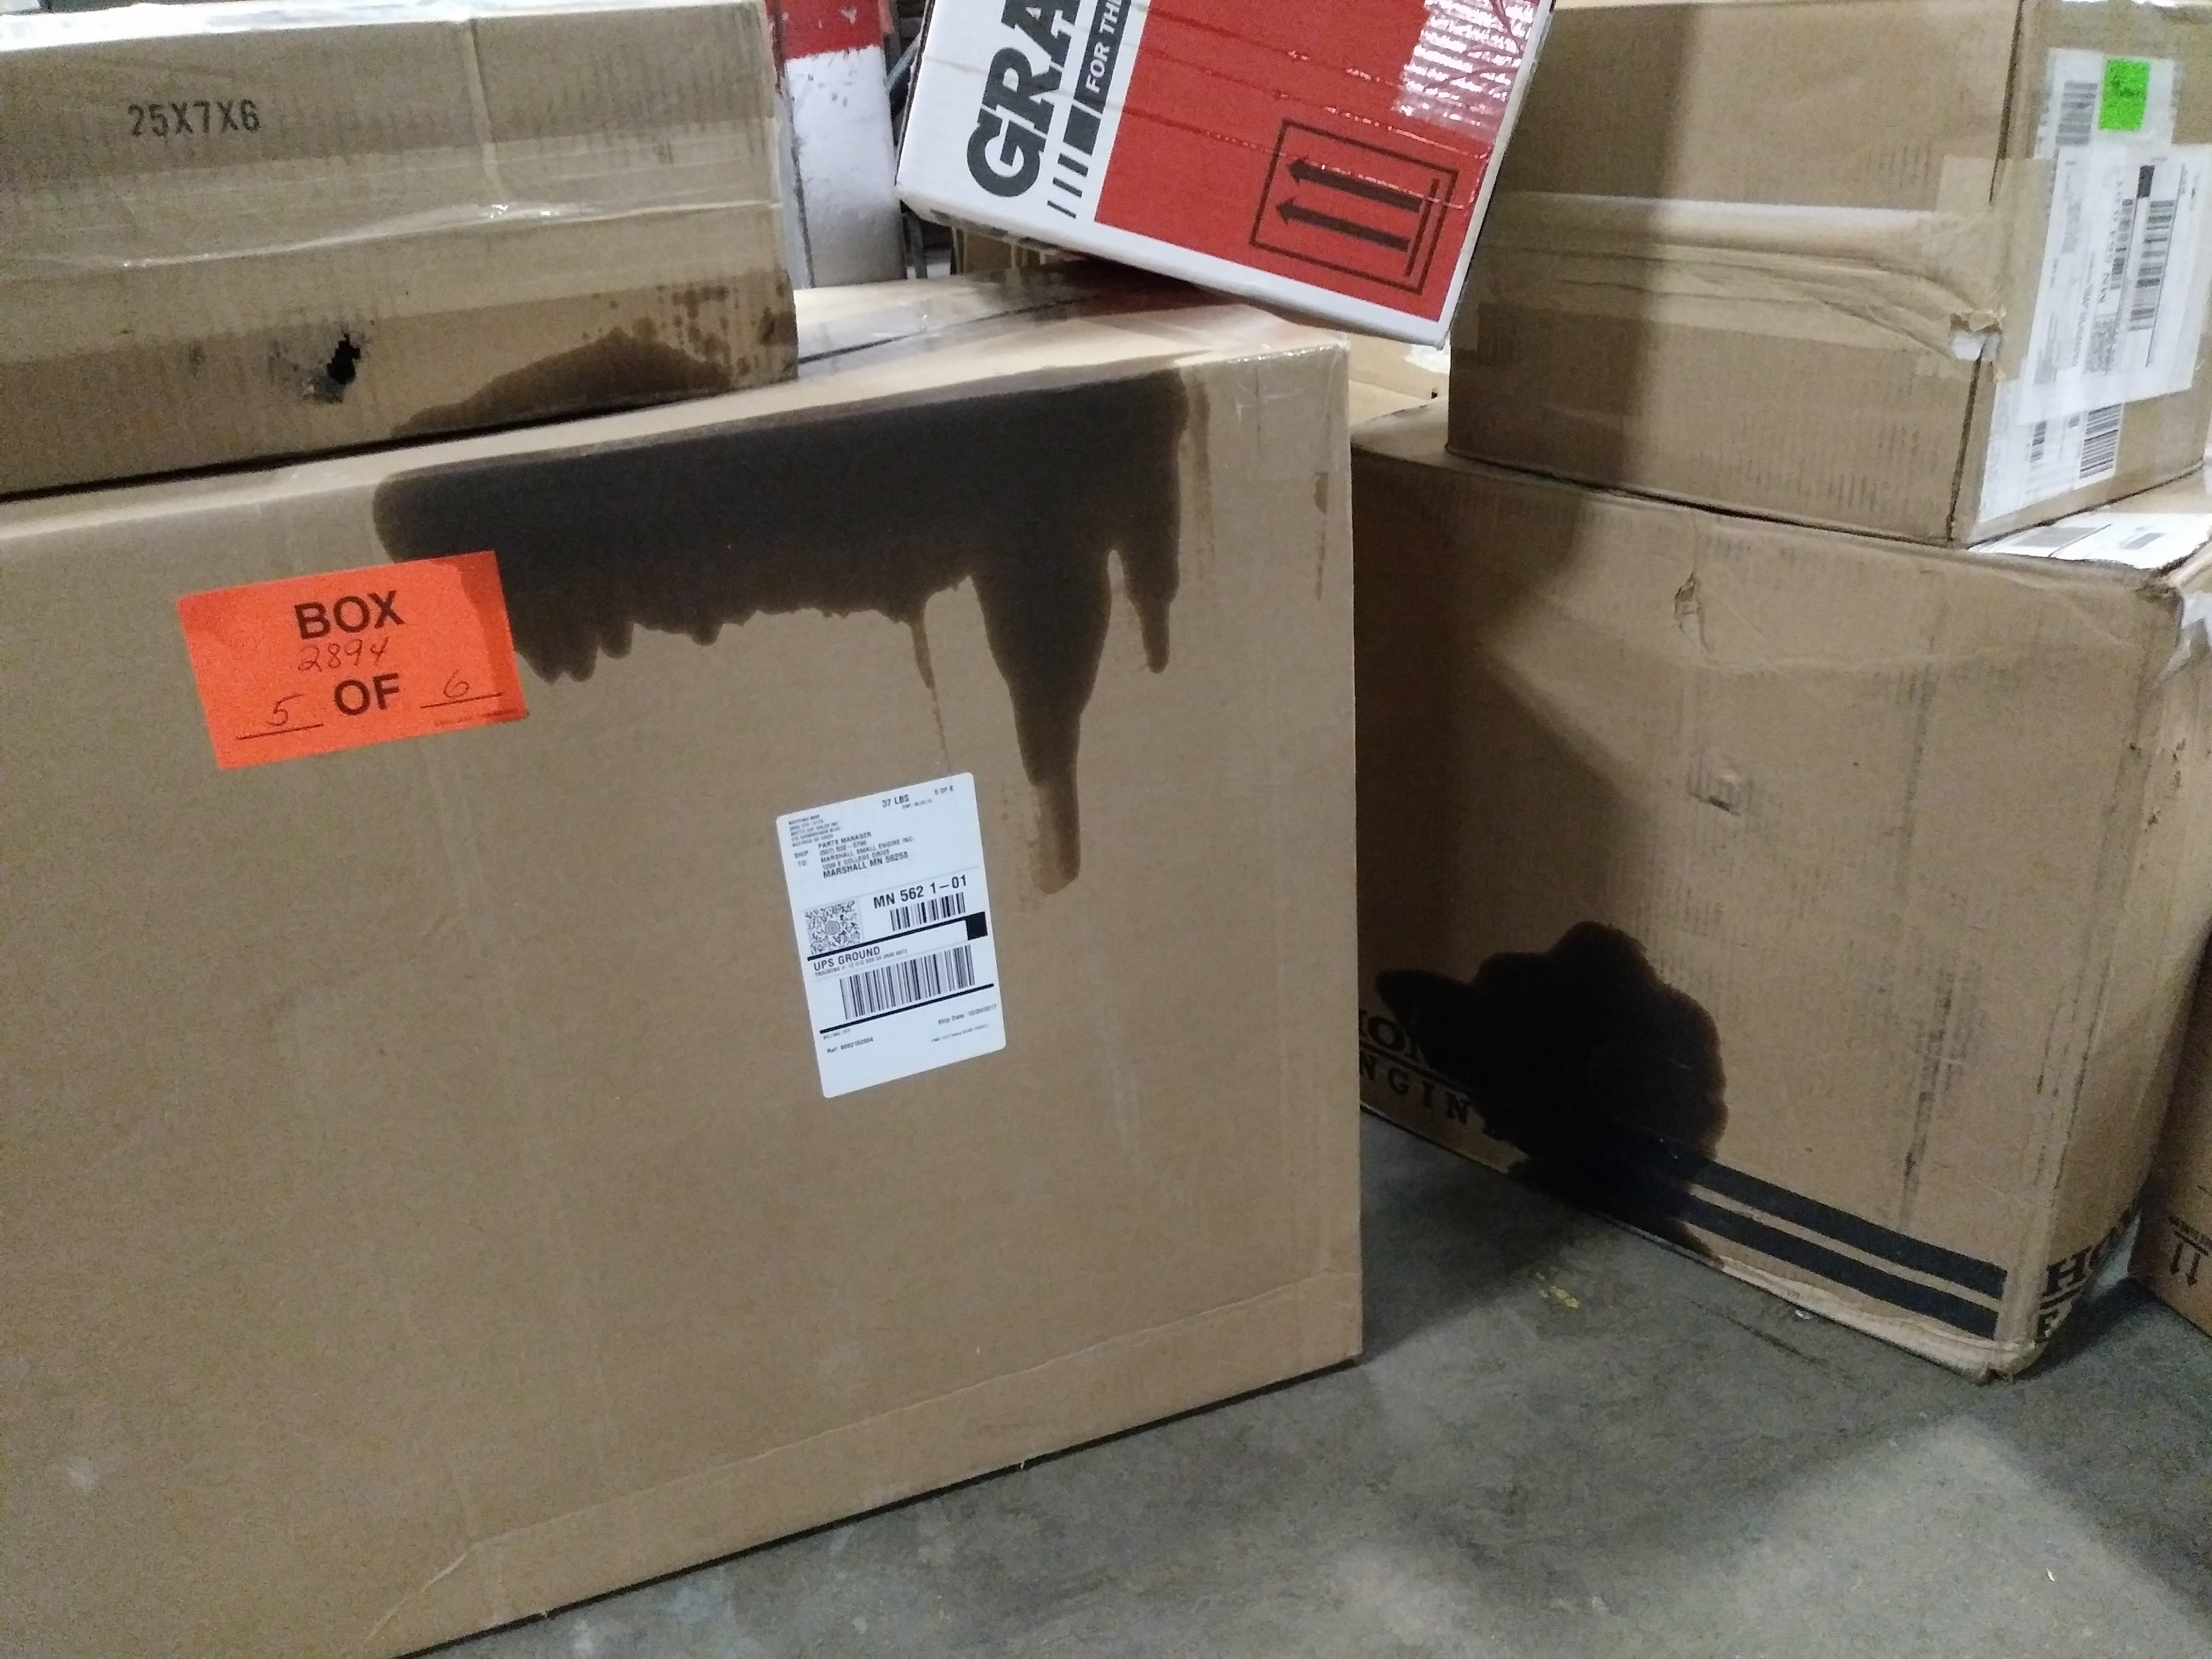
\includegraphics[width=0.4\linewidth]{20171222_020653}
    \caption{Some leakers}
\end{figure}

\subsubsection{Overgoods}
An obvious outcome of an opened package is the contents finding their way outside the confinement of the box. Any item in this case is defined as an "overgood" and should be treated with special handling. 

\begin{itemize}
    \item Notify your supervisor immediately.
    \item If possible, gather the items together. 
    \item Overgood items should be toted together with all captured contents and the original packaging to be delivered to rewrap.
\end{itemize}

\begin{figure}[H]
    \centering
    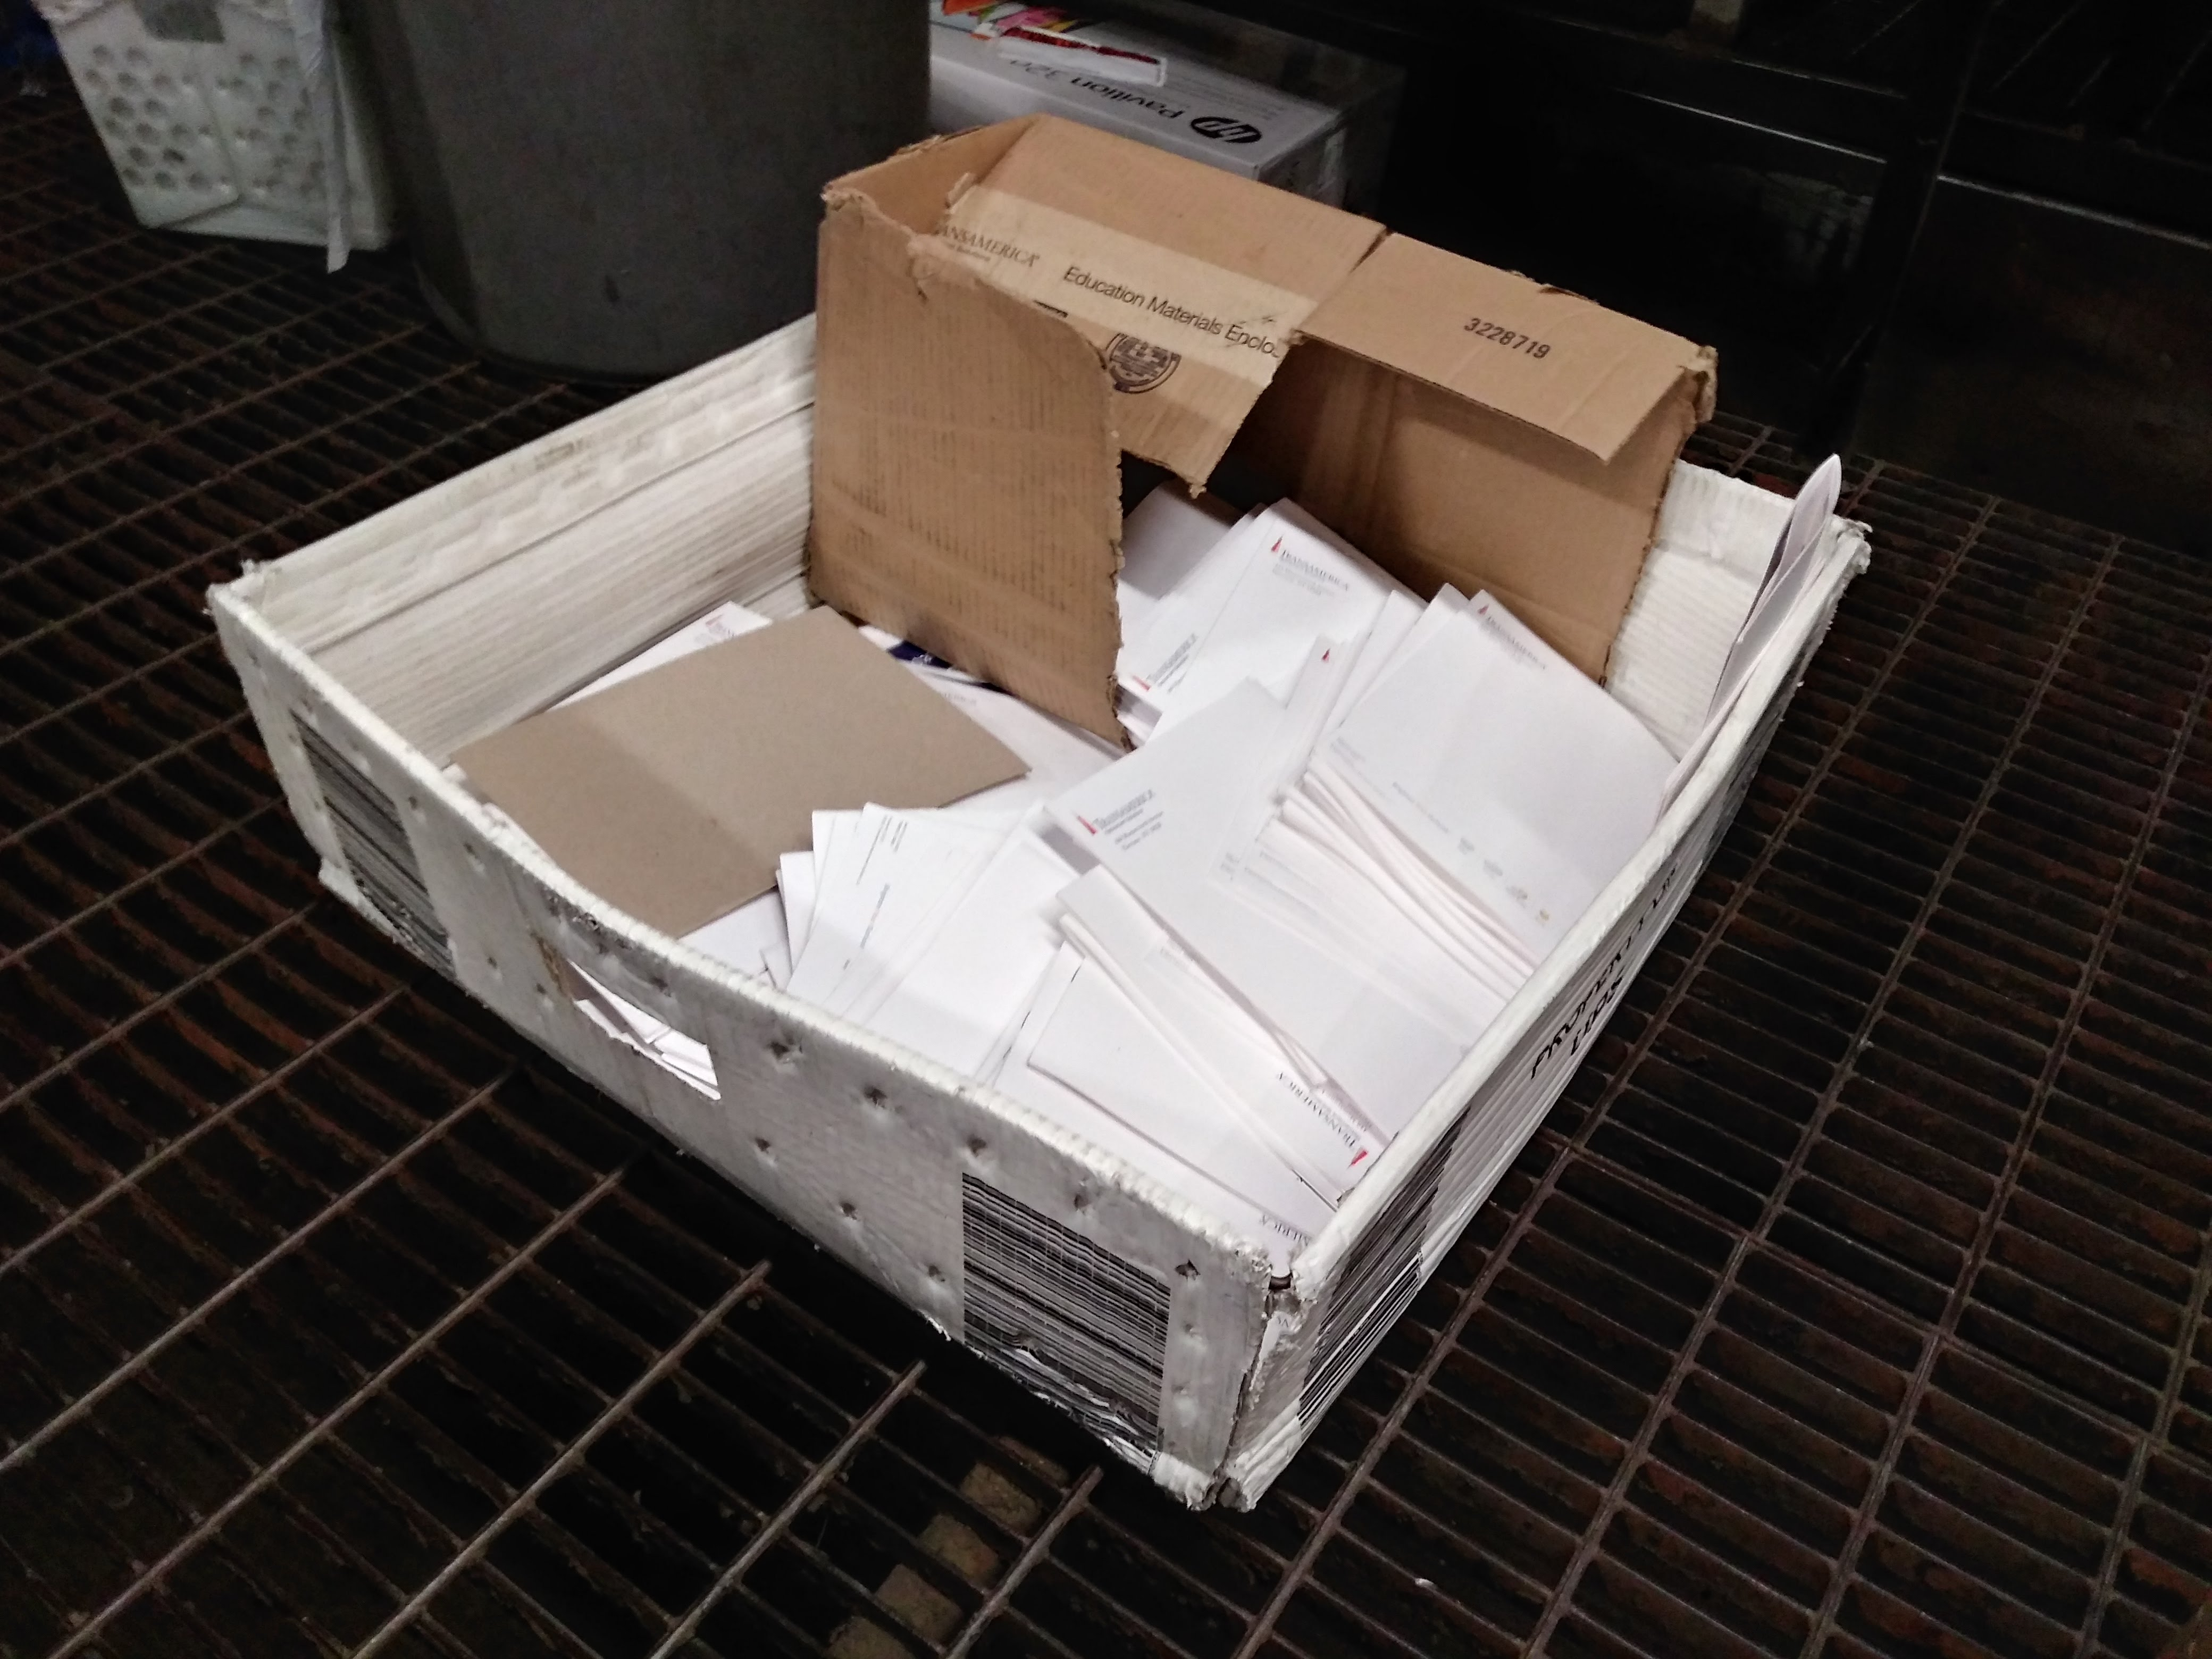
\includegraphics[width=0.5\linewidth]{20171222_013019_HDR}
    \caption{Toted Overgoods}
\end{figure}

\clearpage
\subsection{Irregulars}
Each UPS facility is designed to handle the widest range of package combinations possible. While this covers the majority of our packages, there will always be a percentage of volume that is outside that range of coverage and cannot be handled by the machinery of our facility. These are then brought directly from the unload to the proper outbound door by an irreg driver. 

\begin{itemize}
    \item An irreg = boxes $>$ 70lb, too large to fit on belts, exposed wood/metal, cylinders $>$ 45lb, odd shapes, not wrapped, strong magnets.
    \item It's possible you may need to communicate with an unloader to make sure they are catching irregs at their point of contact.
\end{itemize}

\begin{figure}[H]
\begin{subfigure}{0.5\textwidth}
\centering
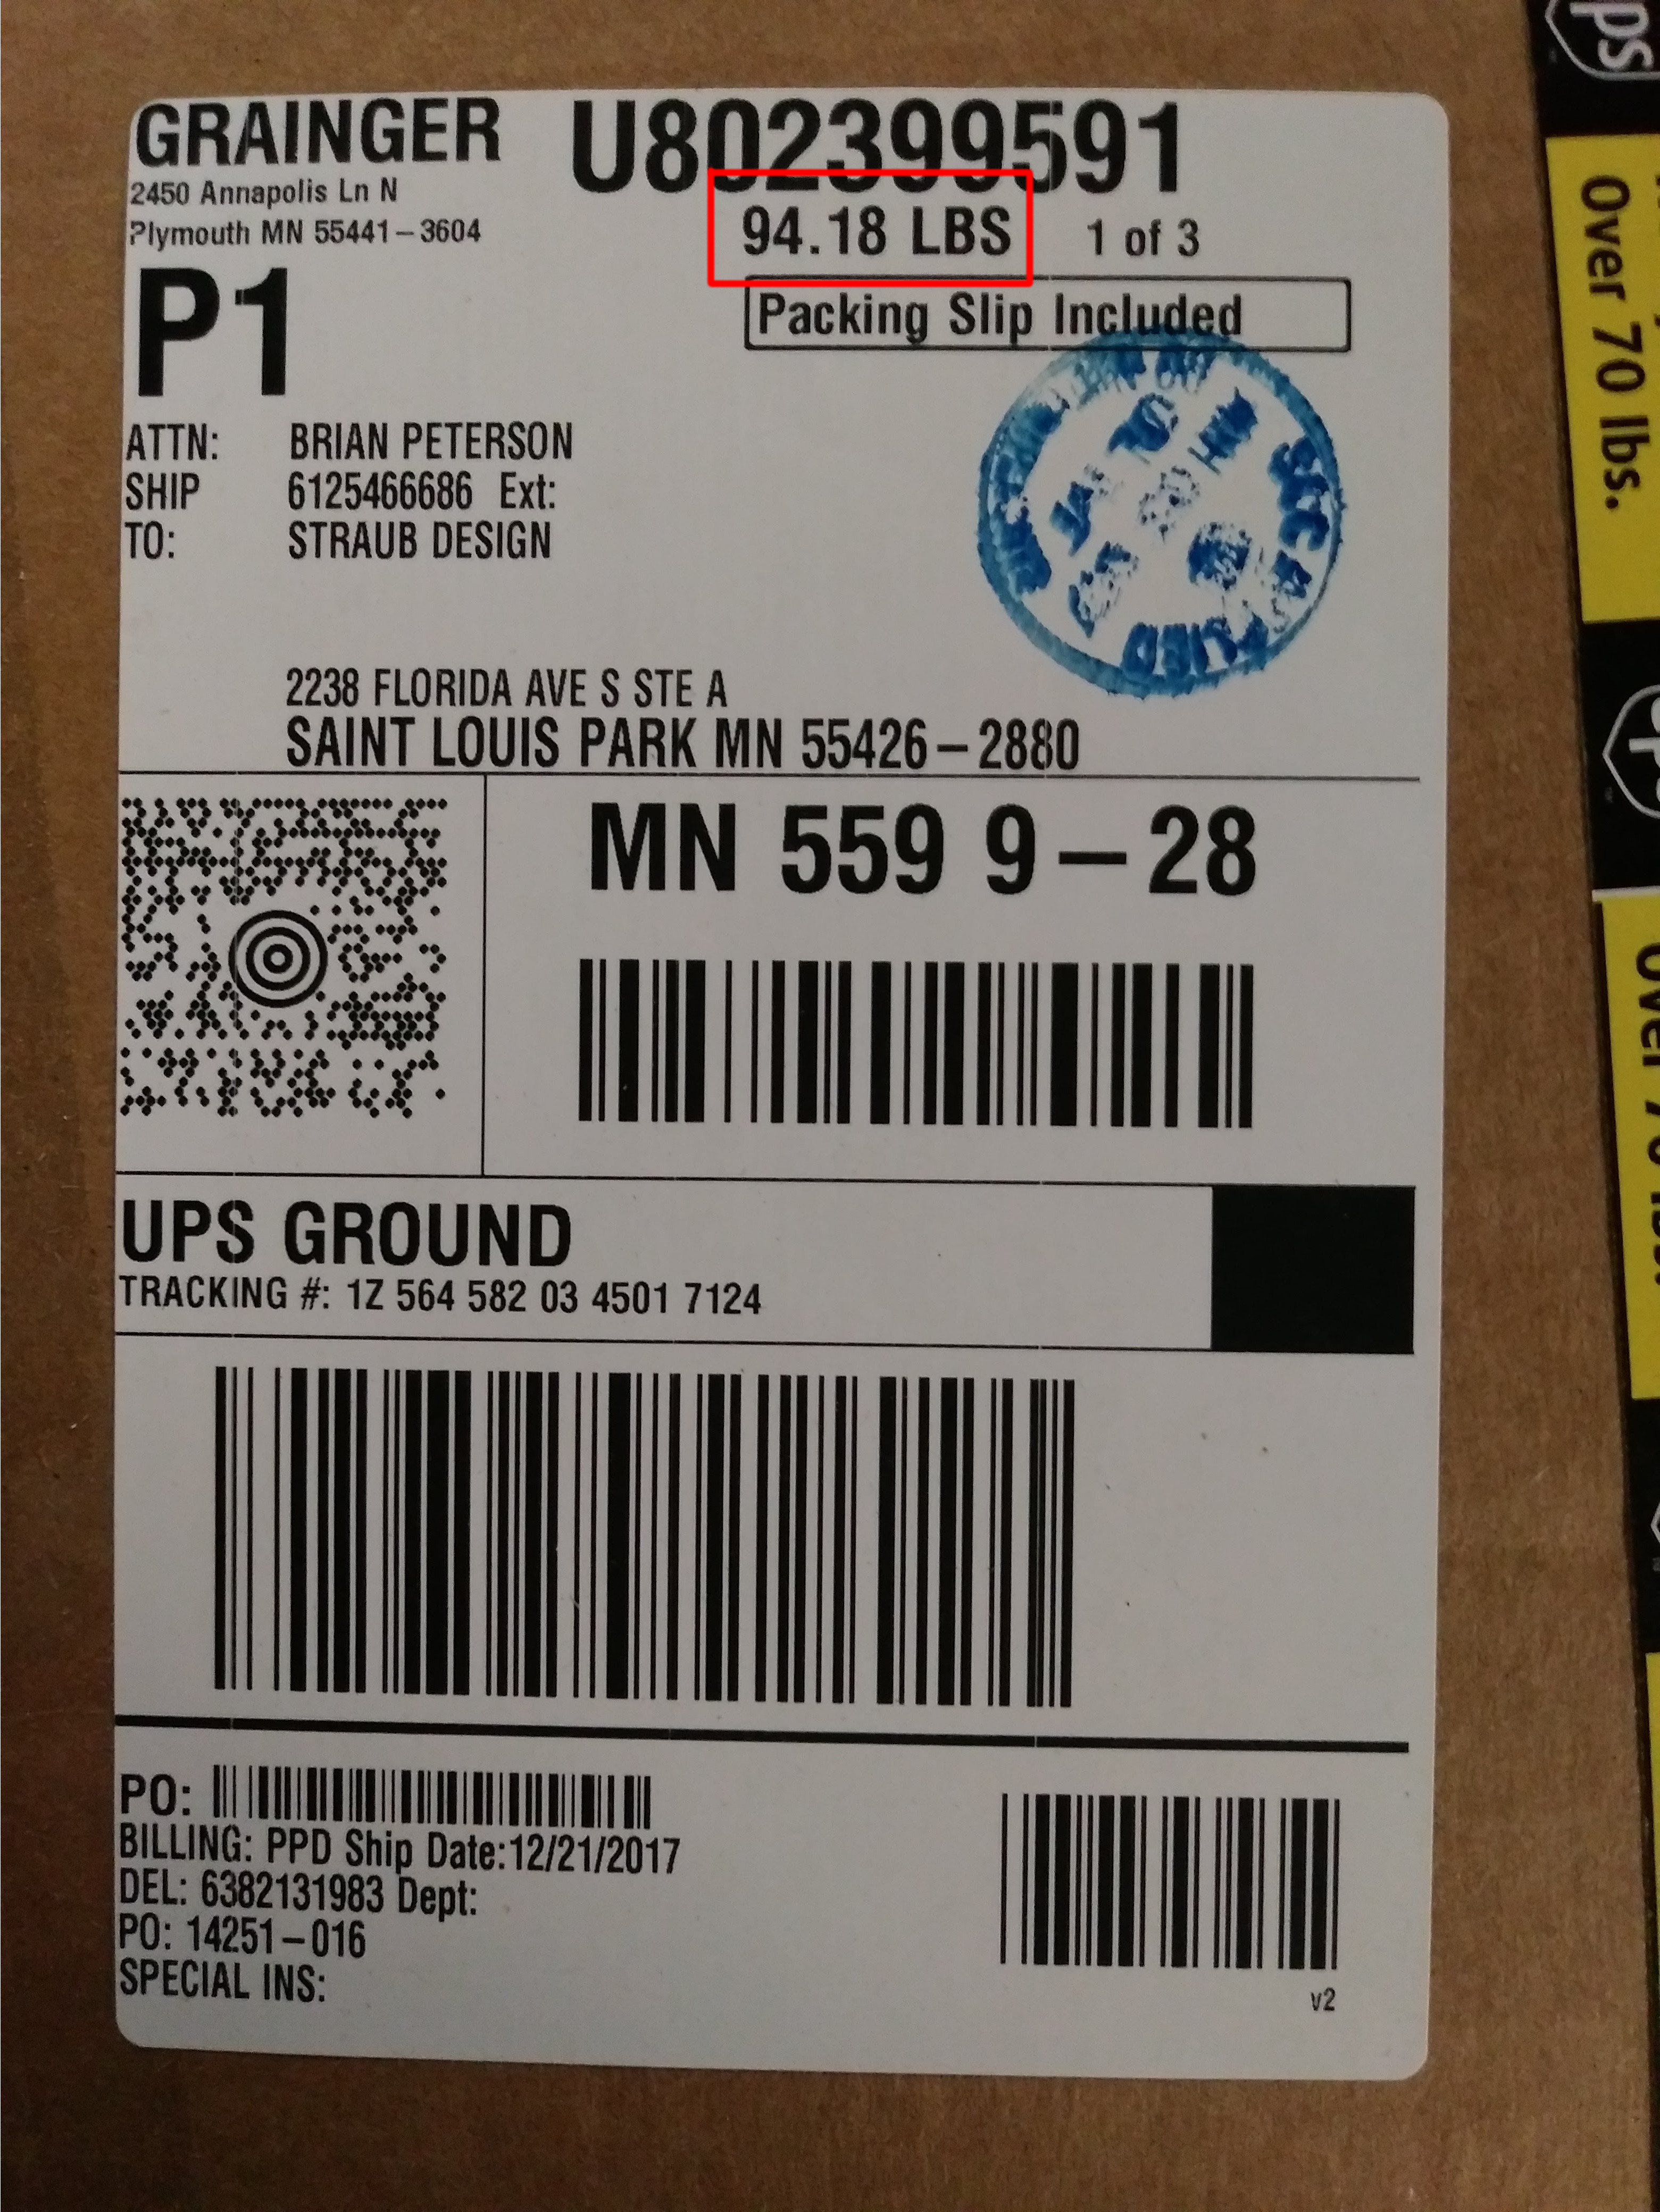
\includegraphics[width=0.4\linewidth]{20171221_203710_irg.jpg} 
\caption{Overweight $>$70lb}
\end{subfigure}
\begin{subfigure}{0.5\textwidth}
\centering
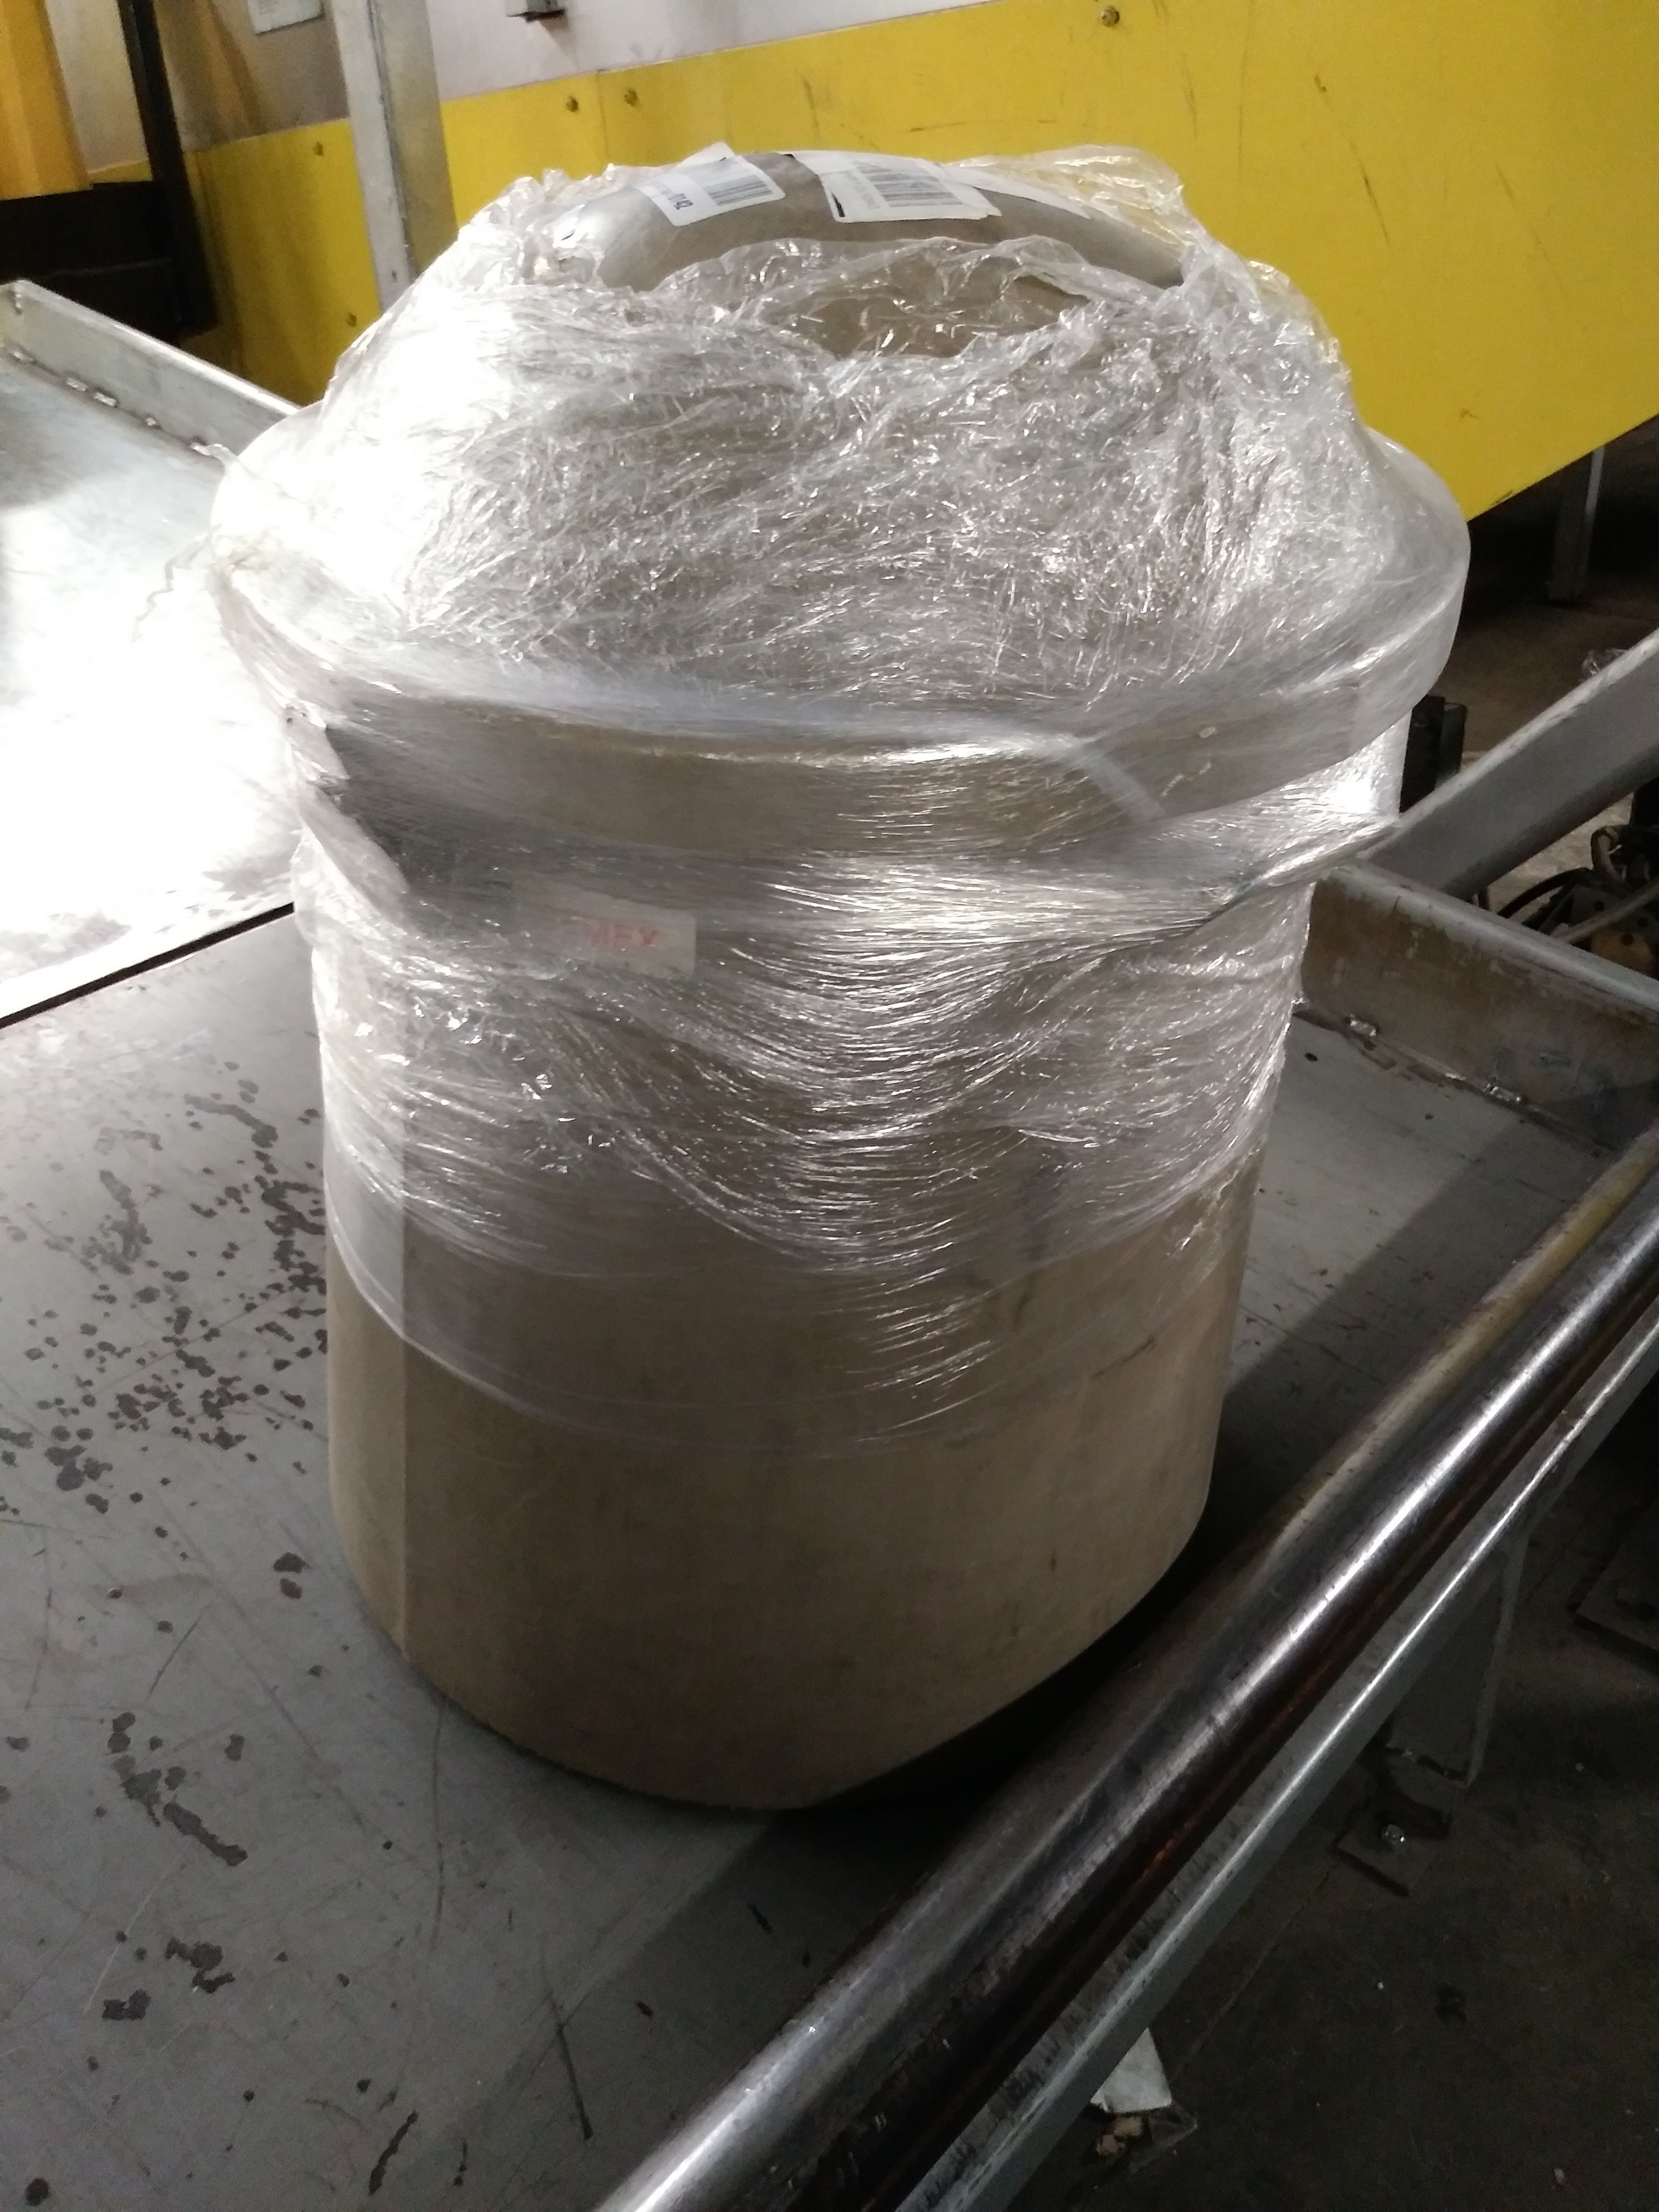
\includegraphics[width=0.4\linewidth]{20171222_022314.jpg}
\caption{Odd Shape}
\end{subfigure}
\begin{subfigure}{0.5\textwidth}
\centering
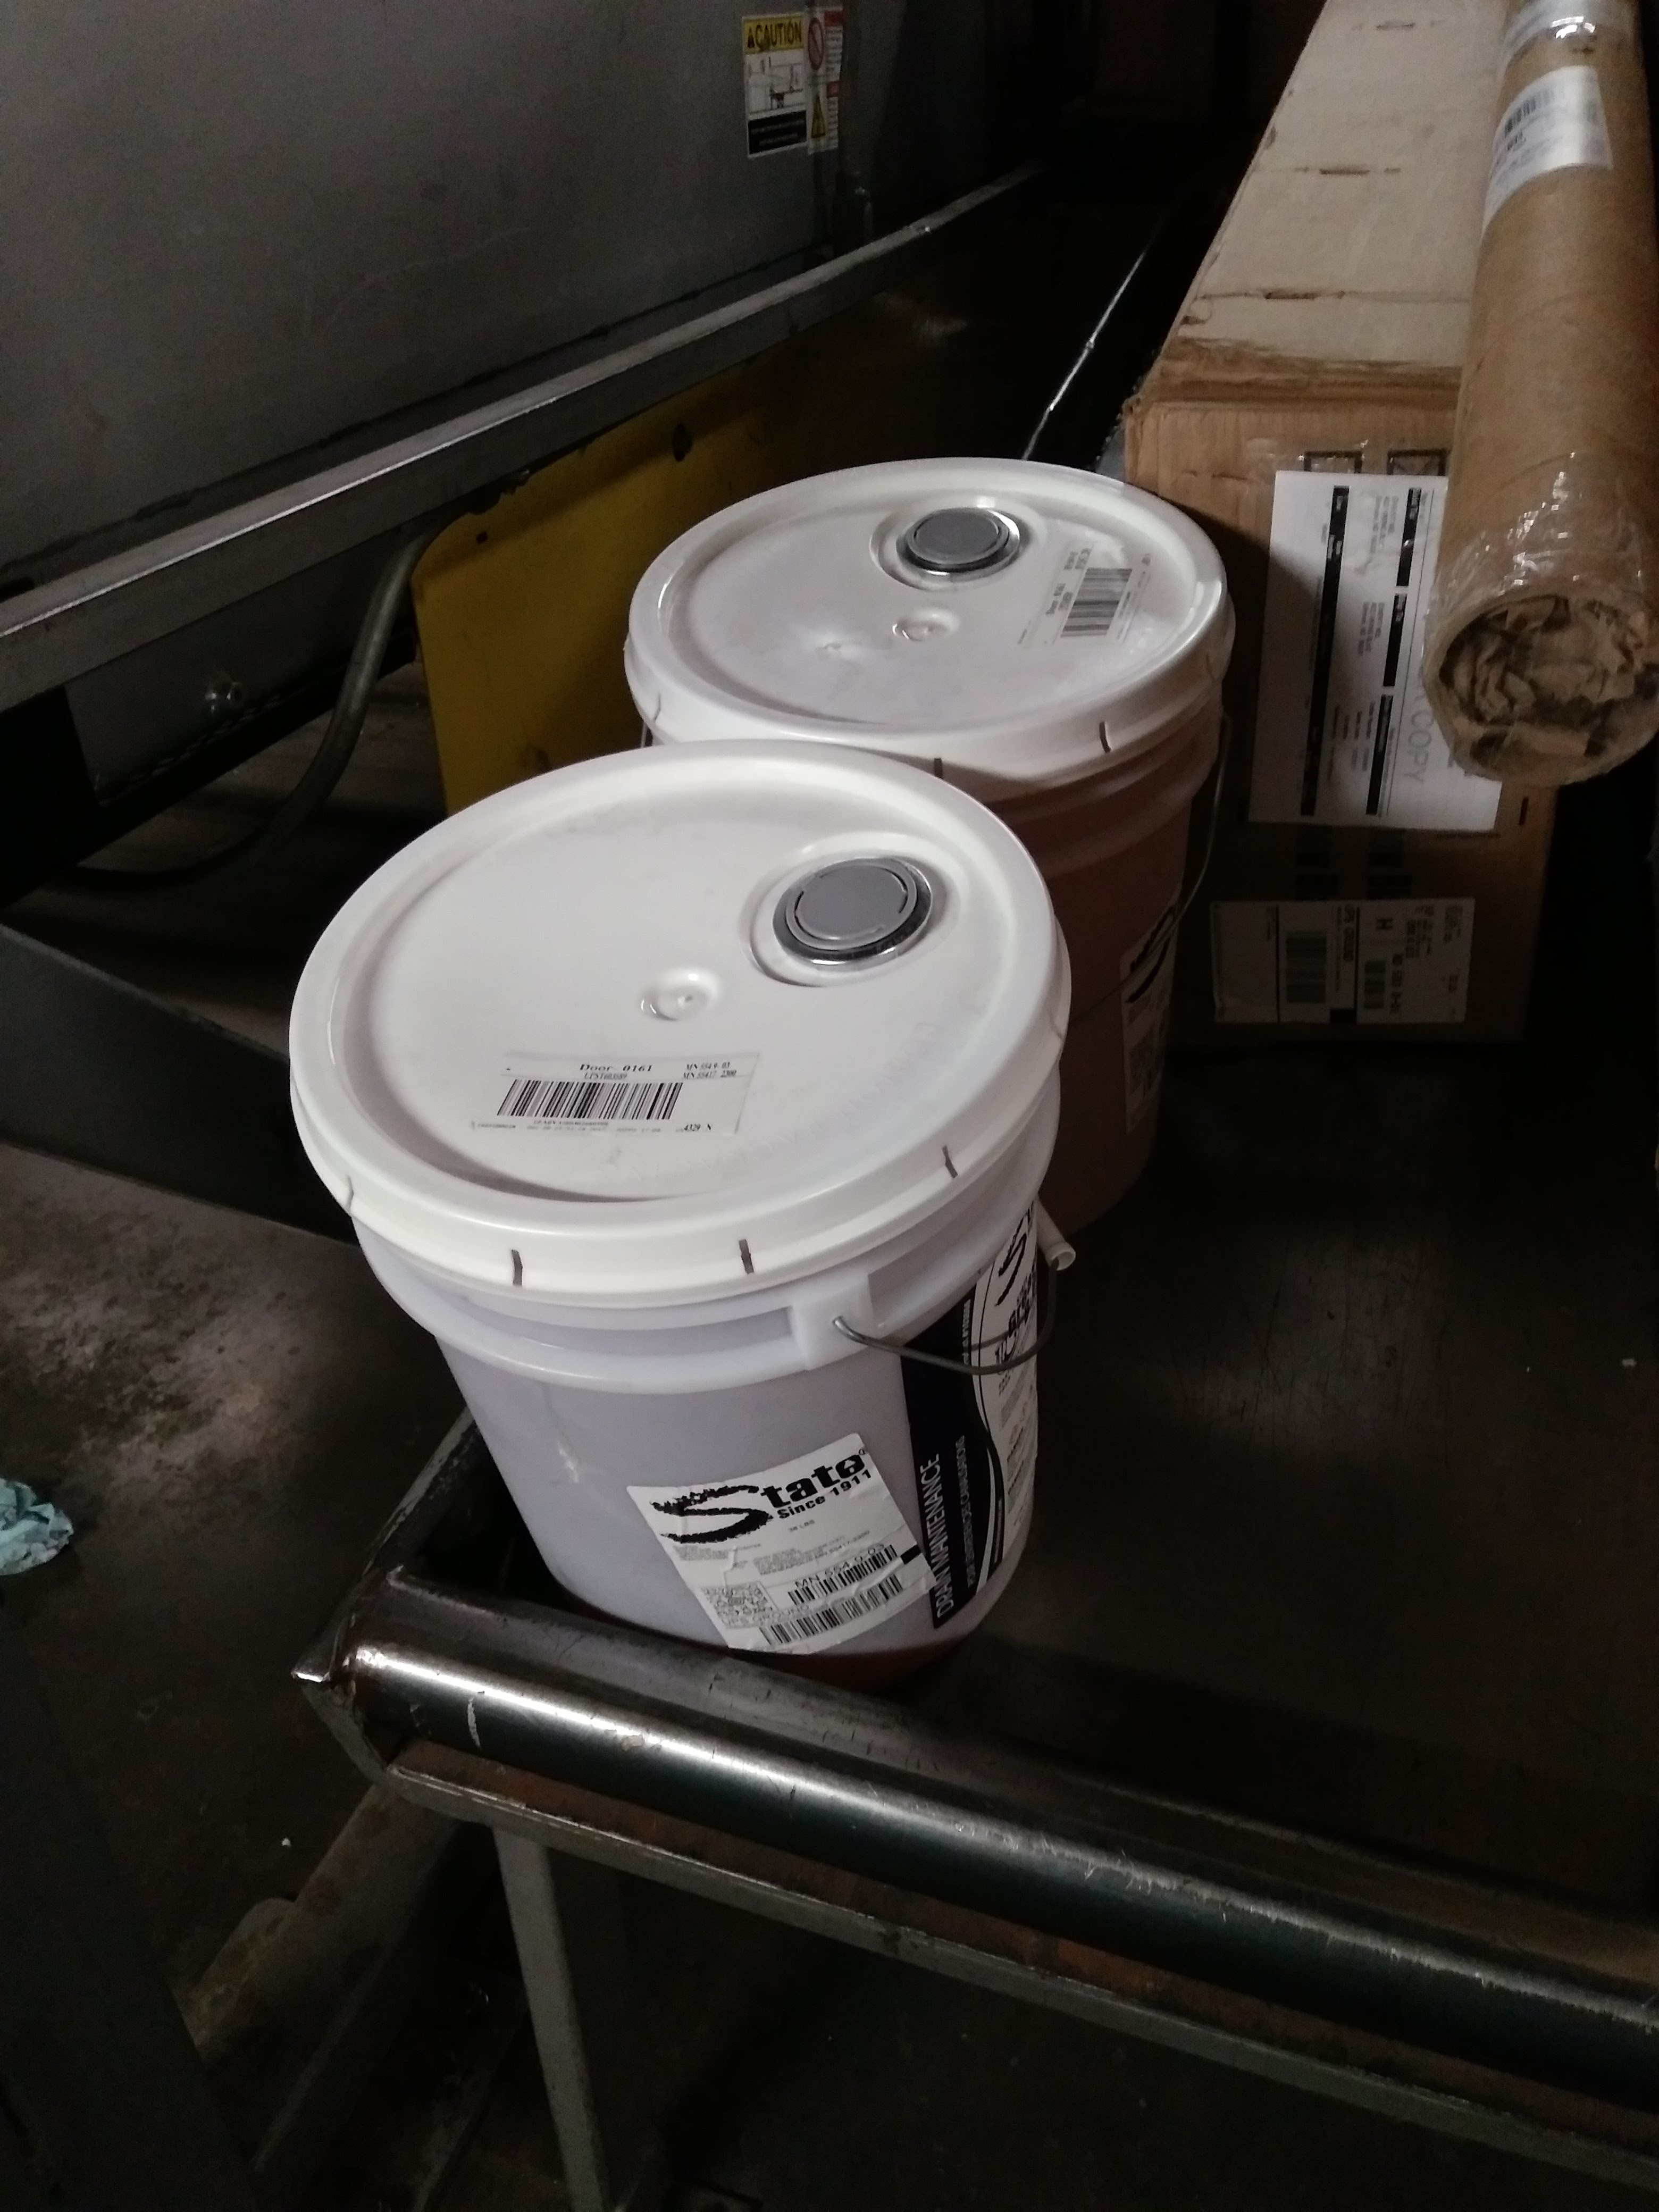
\includegraphics[width=0.4\linewidth]{20171222_022238.jpg}
\caption{Slippery Plastic}
\end{subfigure}
\begin{subfigure}{0.5\textwidth}
\centering
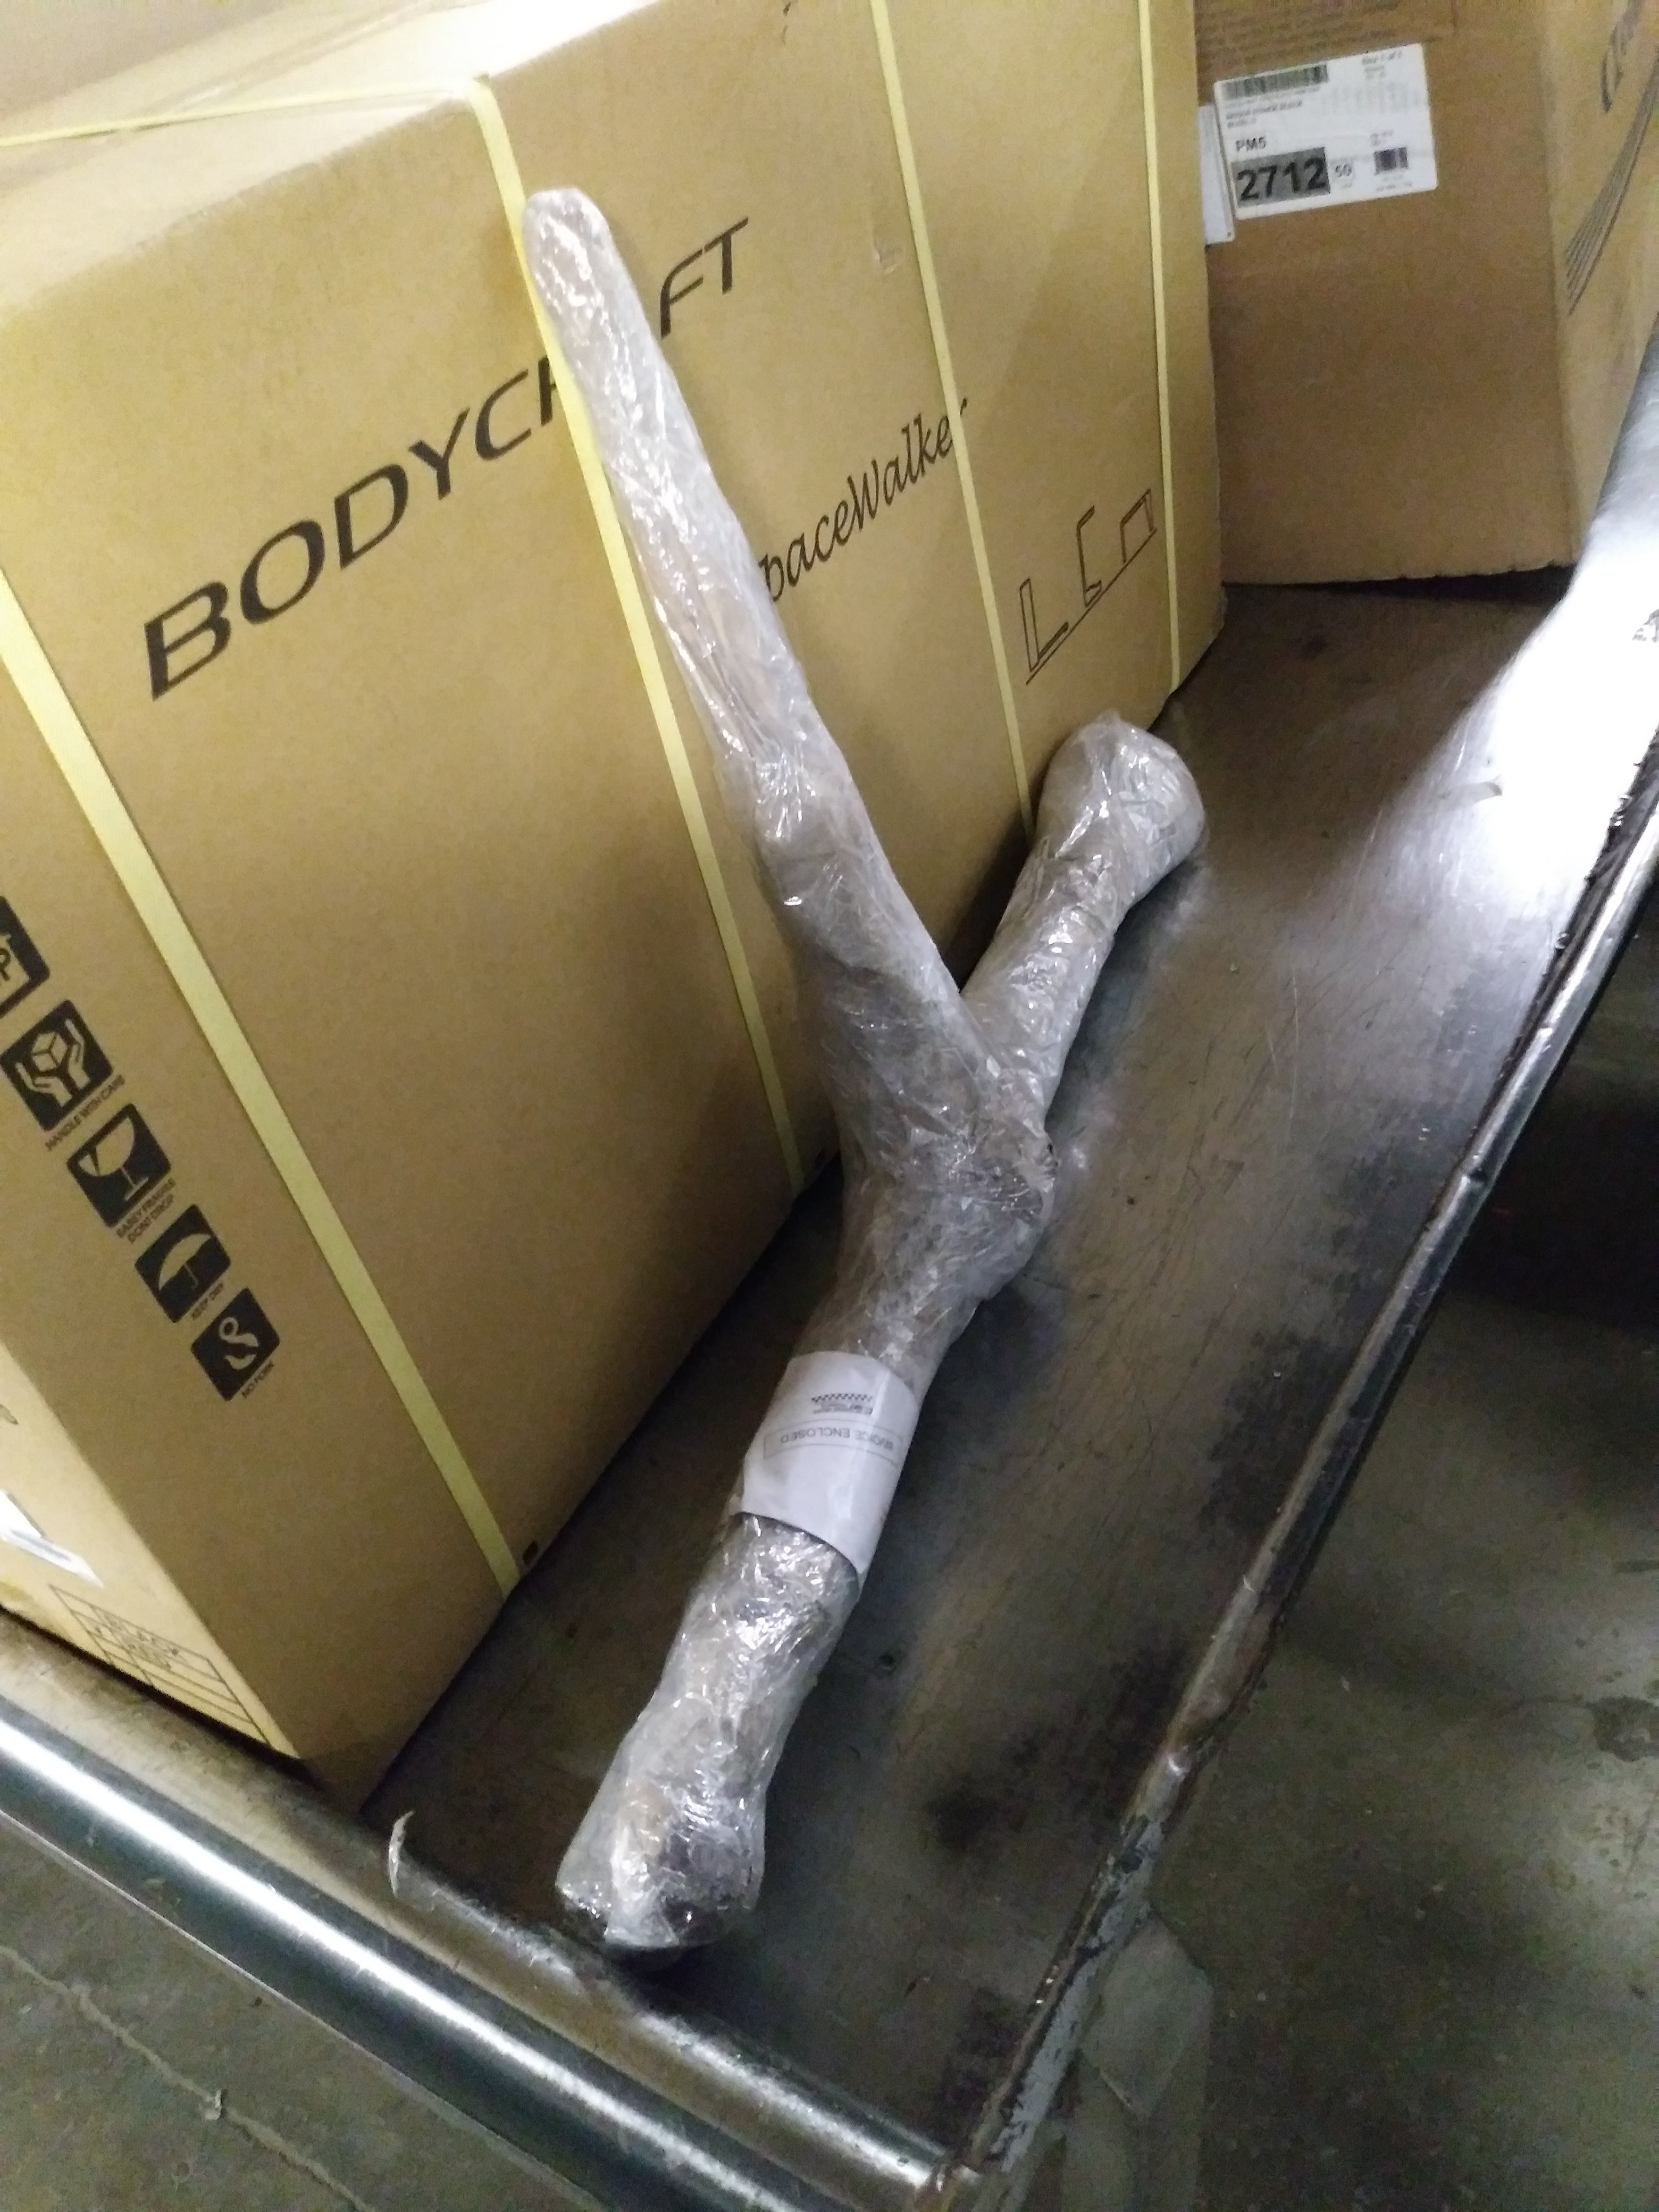
\includegraphics[width=0.4\linewidth]{20171222_022232.jpg}
\caption{Odd Shape}
\end{subfigure}
\begin{subfigure}{0.5\textwidth}
\centering
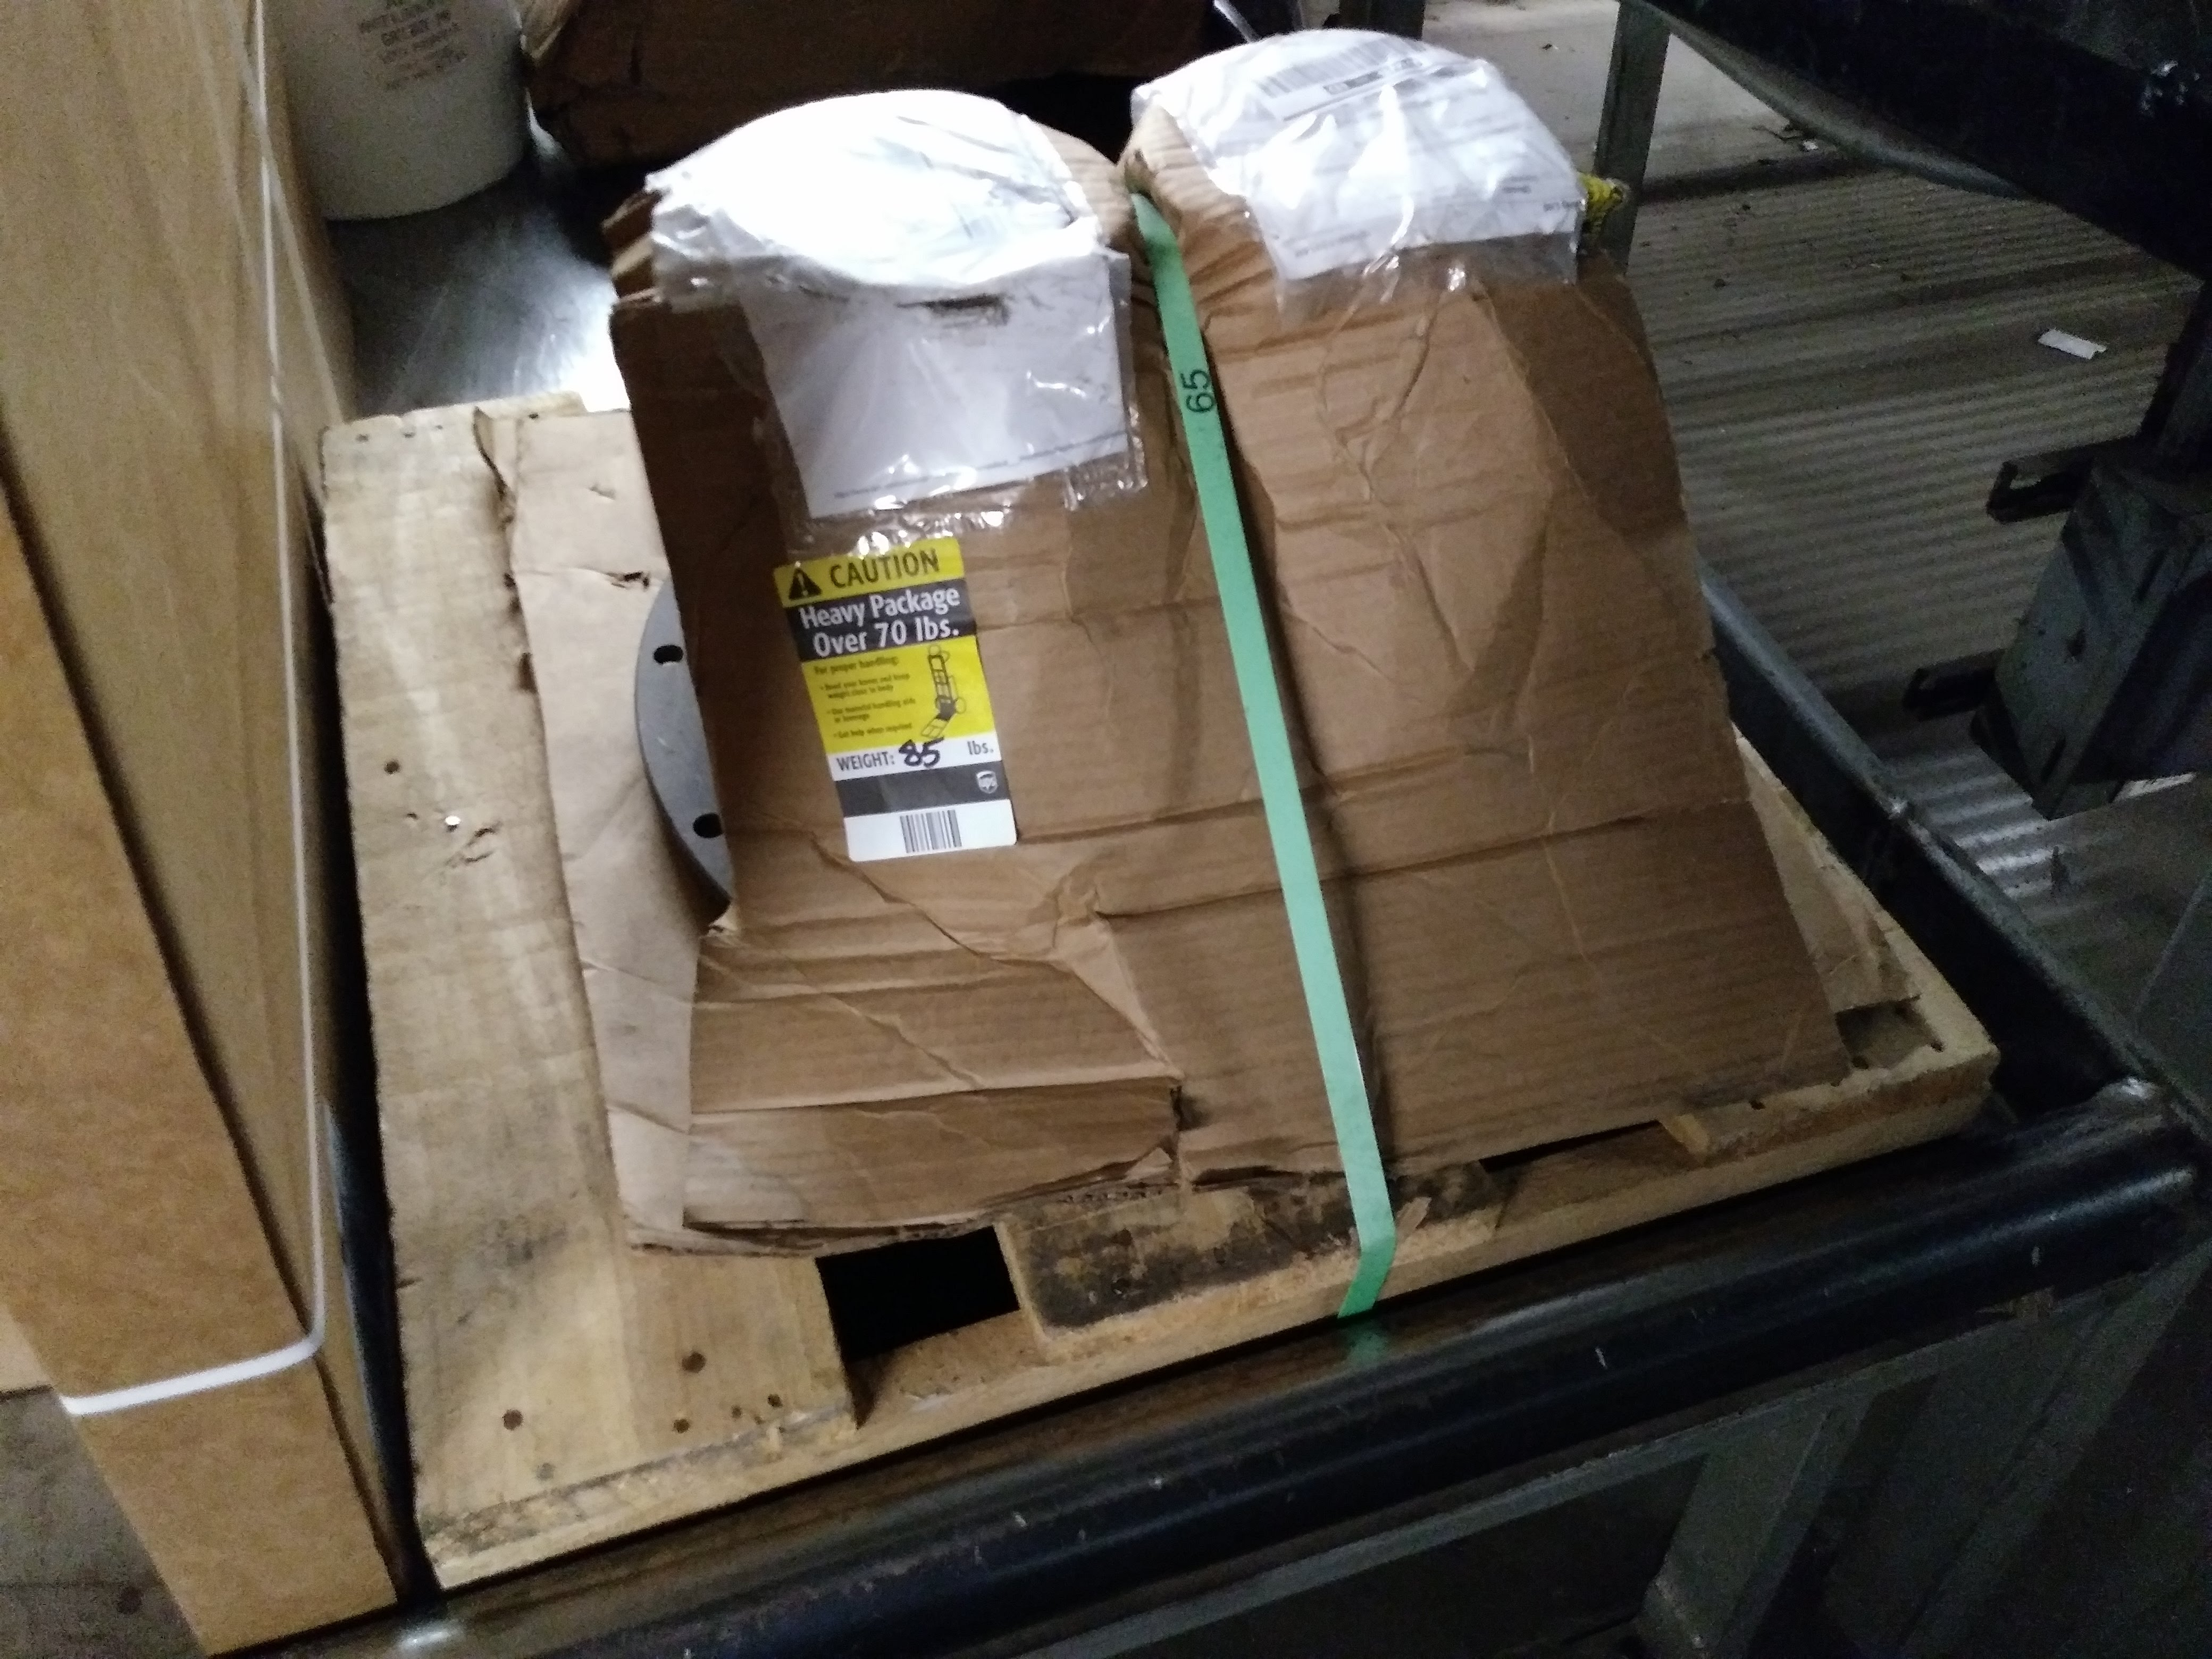
\includegraphics[width=0.4\linewidth]{20171222_022213.jpg}
\caption{Odd Shape/Exposed Wood}
\end{subfigure}
\begin{subfigure}{0.5\textwidth}
\centering
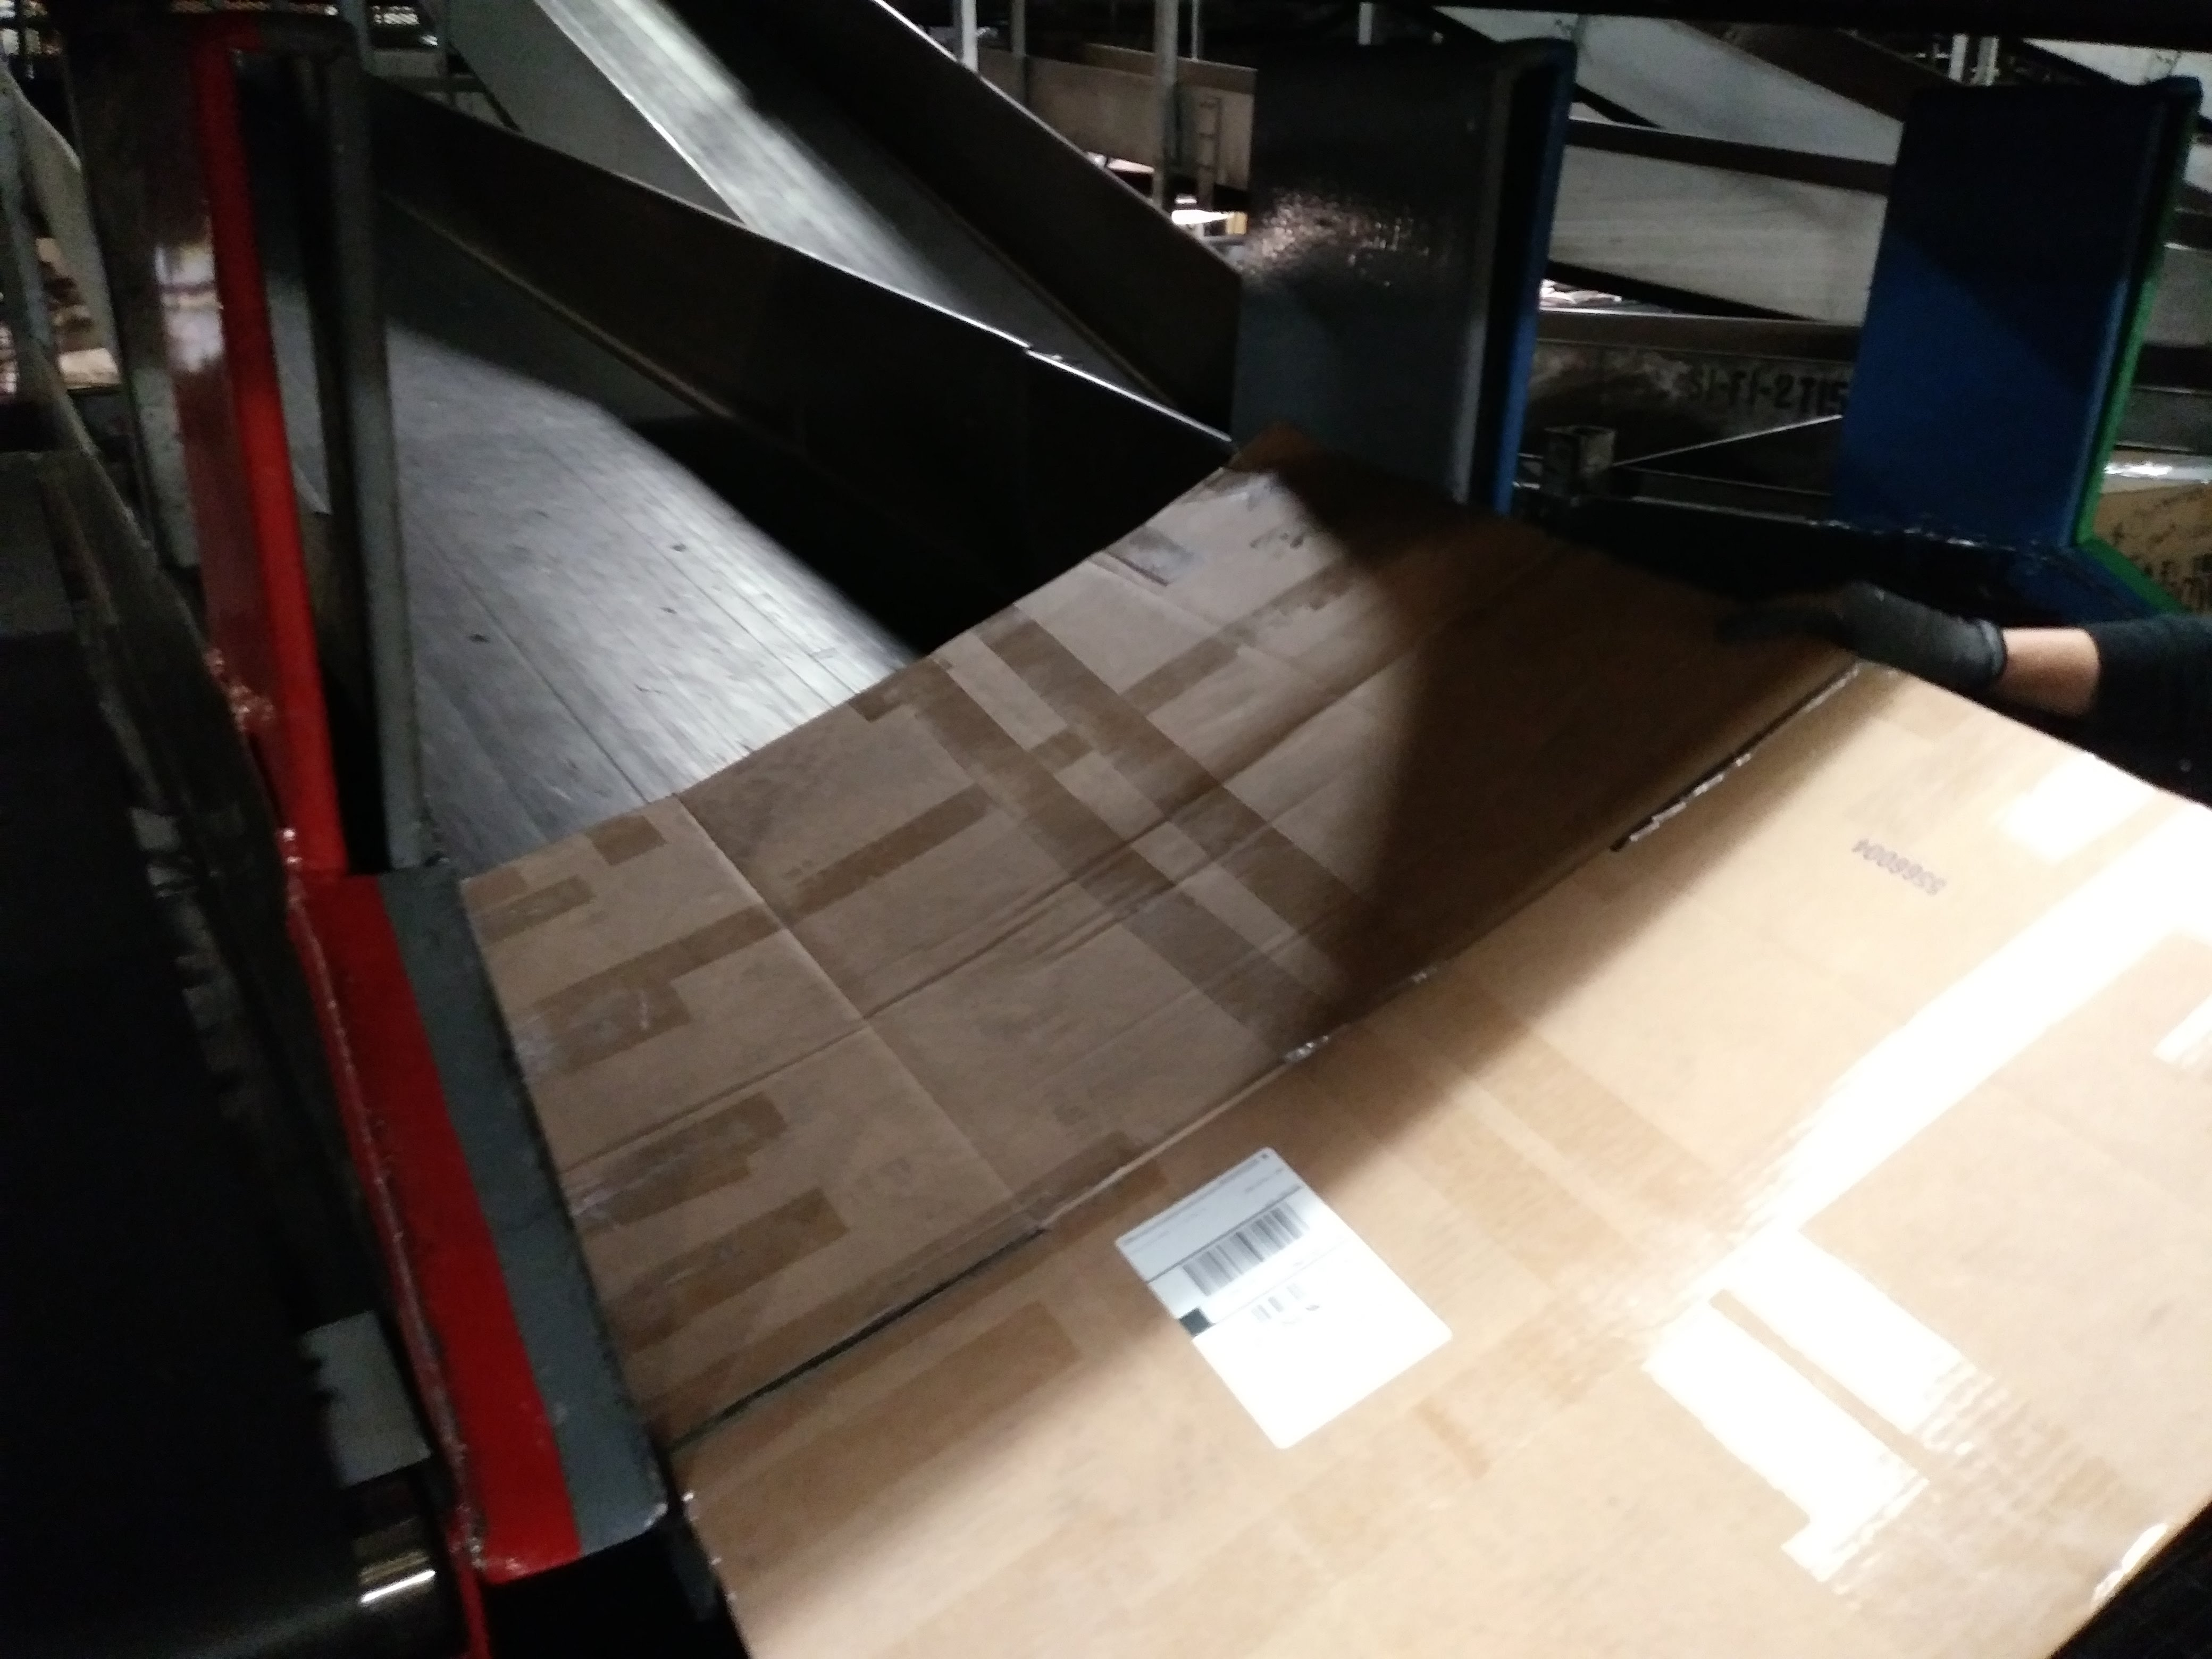
\includegraphics[width=0.4\linewidth]{20171221_175349.jpg}
\caption{Too Big}
\end{subfigure}
\end{figure}
\clearpage



% \subsection{Process Improvements}
% content

% \subsubsection{Face Flow}
% content

% \subsubsection{Positioning}
% content

% \subsubsection{Look Ahead}
% content

% \subsubsection{Division of Labor}
% content


\end{document}

